% Options for packages loaded elsewhere
\PassOptionsToPackage{unicode}{hyperref}
\PassOptionsToPackage{hyphens}{url}
%
\documentclass[
  oneside]{book}
\usepackage{amsmath,amssymb}
\usepackage{iftex}
\ifPDFTeX
  \usepackage[T1]{fontenc}
  \usepackage[utf8]{inputenc}
  \usepackage{textcomp} % provide euro and other symbols
\else % if luatex or xetex
  \usepackage{unicode-math} % this also loads fontspec
  \defaultfontfeatures{Scale=MatchLowercase}
  \defaultfontfeatures[\rmfamily]{Ligatures=TeX,Scale=1}
\fi
\usepackage{lmodern}
\ifPDFTeX\else
  % xetex/luatex font selection
\fi
% Use upquote if available, for straight quotes in verbatim environments
\IfFileExists{upquote.sty}{\usepackage{upquote}}{}
\IfFileExists{microtype.sty}{% use microtype if available
  \usepackage[]{microtype}
  \UseMicrotypeSet[protrusion]{basicmath} % disable protrusion for tt fonts
}{}
\makeatletter
\@ifundefined{KOMAClassName}{% if non-KOMA class
  \IfFileExists{parskip.sty}{%
    \usepackage{parskip}
  }{% else
    \setlength{\parindent}{0pt}
    \setlength{\parskip}{6pt plus 2pt minus 1pt}}
}{% if KOMA class
  \KOMAoptions{parskip=half}}
\makeatother
\usepackage{xcolor}
\usepackage[top=3cm,left=1cm,right=1cm,heightrounded]{geometry}
\usepackage{color}
\usepackage{fancyvrb}
\newcommand{\VerbBar}{|}
\newcommand{\VERB}{\Verb[commandchars=\\\{\}]}
\DefineVerbatimEnvironment{Highlighting}{Verbatim}{commandchars=\\\{\}}
% Add ',fontsize=\small' for more characters per line
\usepackage{framed}
\definecolor{shadecolor}{RGB}{248,248,248}
\newenvironment{Shaded}{\begin{snugshade}}{\end{snugshade}}
\newcommand{\AlertTok}[1]{\textcolor[rgb]{0.94,0.16,0.16}{#1}}
\newcommand{\AnnotationTok}[1]{\textcolor[rgb]{0.56,0.35,0.01}{\textbf{\textit{#1}}}}
\newcommand{\AttributeTok}[1]{\textcolor[rgb]{0.77,0.63,0.00}{#1}}
\newcommand{\BaseNTok}[1]{\textcolor[rgb]{0.00,0.00,0.81}{#1}}
\newcommand{\BuiltInTok}[1]{#1}
\newcommand{\CharTok}[1]{\textcolor[rgb]{0.31,0.60,0.02}{#1}}
\newcommand{\CommentTok}[1]{\textcolor[rgb]{0.56,0.35,0.01}{\textit{#1}}}
\newcommand{\CommentVarTok}[1]{\textcolor[rgb]{0.56,0.35,0.01}{\textbf{\textit{#1}}}}
\newcommand{\ConstantTok}[1]{\textcolor[rgb]{0.00,0.00,0.00}{#1}}
\newcommand{\ControlFlowTok}[1]{\textcolor[rgb]{0.13,0.29,0.53}{\textbf{#1}}}
\newcommand{\DataTypeTok}[1]{\textcolor[rgb]{0.13,0.29,0.53}{#1}}
\newcommand{\DecValTok}[1]{\textcolor[rgb]{0.00,0.00,0.81}{#1}}
\newcommand{\DocumentationTok}[1]{\textcolor[rgb]{0.56,0.35,0.01}{\textbf{\textit{#1}}}}
\newcommand{\ErrorTok}[1]{\textcolor[rgb]{0.64,0.00,0.00}{\textbf{#1}}}
\newcommand{\ExtensionTok}[1]{#1}
\newcommand{\FloatTok}[1]{\textcolor[rgb]{0.00,0.00,0.81}{#1}}
\newcommand{\FunctionTok}[1]{\textcolor[rgb]{0.00,0.00,0.00}{#1}}
\newcommand{\ImportTok}[1]{#1}
\newcommand{\InformationTok}[1]{\textcolor[rgb]{0.56,0.35,0.01}{\textbf{\textit{#1}}}}
\newcommand{\KeywordTok}[1]{\textcolor[rgb]{0.13,0.29,0.53}{\textbf{#1}}}
\newcommand{\NormalTok}[1]{#1}
\newcommand{\OperatorTok}[1]{\textcolor[rgb]{0.81,0.36,0.00}{\textbf{#1}}}
\newcommand{\OtherTok}[1]{\textcolor[rgb]{0.56,0.35,0.01}{#1}}
\newcommand{\PreprocessorTok}[1]{\textcolor[rgb]{0.56,0.35,0.01}{\textit{#1}}}
\newcommand{\RegionMarkerTok}[1]{#1}
\newcommand{\SpecialCharTok}[1]{\textcolor[rgb]{0.00,0.00,0.00}{#1}}
\newcommand{\SpecialStringTok}[1]{\textcolor[rgb]{0.31,0.60,0.02}{#1}}
\newcommand{\StringTok}[1]{\textcolor[rgb]{0.31,0.60,0.02}{#1}}
\newcommand{\VariableTok}[1]{\textcolor[rgb]{0.00,0.00,0.00}{#1}}
\newcommand{\VerbatimStringTok}[1]{\textcolor[rgb]{0.31,0.60,0.02}{#1}}
\newcommand{\WarningTok}[1]{\textcolor[rgb]{0.56,0.35,0.01}{\textbf{\textit{#1}}}}
\usepackage{longtable,booktabs,array}
\usepackage{calc} % for calculating minipage widths
% Correct order of tables after \paragraph or \subparagraph
\usepackage{etoolbox}
\makeatletter
\patchcmd\longtable{\par}{\if@noskipsec\mbox{}\fi\par}{}{}
\makeatother
% Allow footnotes in longtable head/foot
\IfFileExists{footnotehyper.sty}{\usepackage{footnotehyper}}{\usepackage{footnote}}
\makesavenoteenv{longtable}
\usepackage{graphicx}
\makeatletter
\def\maxwidth{\ifdim\Gin@nat@width>\linewidth\linewidth\else\Gin@nat@width\fi}
\def\maxheight{\ifdim\Gin@nat@height>\textheight\textheight\else\Gin@nat@height\fi}
\makeatother
% Scale images if necessary, so that they will not overflow the page
% margins by default, and it is still possible to overwrite the defaults
% using explicit options in \includegraphics[width, height, ...]{}
\setkeys{Gin}{width=\maxwidth,height=\maxheight,keepaspectratio}
% Set default figure placement to htbp
\makeatletter
\def\fps@figure{htbp}
\makeatother
\setlength{\emergencystretch}{3em} % prevent overfull lines
\providecommand{\tightlist}{%
  \setlength{\itemsep}{0pt}\setlength{\parskip}{0pt}}
\setcounter{secnumdepth}{5}
\usepackage{booktabs}
\ifLuaTeX
  \usepackage{selnolig}  % disable illegal ligatures
\fi
\usepackage[]{natbib}
\bibliographystyle{plainnat}
\IfFileExists{bookmark.sty}{\usepackage{bookmark}}{\usepackage{hyperref}}
\IfFileExists{xurl.sty}{\usepackage{xurl}}{} % add URL line breaks if available
\urlstyle{same}
\hypersetup{
  pdftitle={STAD70 Course Work},
  pdfauthor={Richard Ye},
  hidelinks,
  pdfcreator={LaTeX via pandoc}}

\title{STAD70 Course Work}
\author{Richard Ye}
\date{}

\begin{document}
\maketitle

{
\setcounter{tocdepth}{1}
\tableofcontents
}
\hypertarget{introduction}{%
\chapter{Introduction}\label{introduction}}

Work from the STAD70 course taken Winter 2023.

\hypertarget{financial-data-and-returns}{%
\chapter{Financial Data and Returns}\label{financial-data-and-returns}}

\url{https://richardye101.github.io/STAD70/}

\begin{itemize}
\tightlist
\item
  Prices of financial instruments (stocks, bonds, futures, options, etc)
\item
\item
  LIBOR: London Inter-Bank Offered Rate

  \begin{itemize}
  \tightlist
  \item
    Avg interest rate that major London Banks would charge when borrowing from each other
  \end{itemize}
\item
  FX Rates: Decentralized market that sets currency prices
\end{itemize}

There are two types of \emph{raw (tick)} data:

\begin{itemize}
\tightlist
\item
  \textbf{Quote data}

  \begin{itemize}
  \tightlist
  \item
    Record of bid/ask prices from the order book, usually just the top \(N\) lines of the order book on the bid and ask sides
  \end{itemize}
\item
  \textbf{Trade data}

  \begin{itemize}
  \tightlist
  \item
    Trade records (filled orders)
  \end{itemize}
\end{itemize}

Data that is identified using time:

\begin{itemize}
\tightlist
\item
  \textbf{Intraday Data}

  \begin{itemize}
  \tightlist
  \item
    Data of the most current bids/asks, last price, volume etc
  \item
    Describes the data of a stock within a given day
  \end{itemize}
\item
  \textbf{Daily data}

  \begin{itemize}
  \tightlist
  \item
    For longer term analysis
  \end{itemize}
\end{itemize}

\hypertarget{trading}{%
\section{Trading}\label{trading}}

There are two types:

\begin{itemize}
\tightlist
\item
  \textbf{OTC (Over the counter)}

  \begin{itemize}
  \tightlist
  \item
    Negotiated and traded directly between parties, not for the public to bid on
  \end{itemize}
\item
  \textbf{Through an Exchange}

  \begin{itemize}
  \tightlist
  \item
    The TSX, NYSE, LSE (London)
  \item
    Uses an \textbf{auction} system where there are many potential buyers and sellers
  \item
    Uses a \textbf{continuous double auction (CDA)}, where the bids and asks are matched in real-time to determine which trades to execute.

    \begin{itemize}
    \tightlist
    \item
      A matching order (bid \(\geq\) ask) is executed right away
    \item
      Outstanding orders are maintained in an \textbf{order book}
    \end{itemize}
  \end{itemize}
\end{itemize}

\hypertarget{order-types}{%
\section{Order Types}\label{order-types}}

\begin{itemize}
\tightlist
\item
  Limit order: buy/sell are no more/les than a specified price

  \begin{itemize}
  \tightlist
  \item
    It is maintained in the order book if not filled immediately
  \end{itemize}
\item
  Market order: buy/sell at the current market price immediately

  \begin{itemize}
  \tightlist
  \item
    No control over the price at which the order will execute
  \end{itemize}
\item
  Iceberg order: Only a portion of the total (giant) order is displayed in the order book, and when it is filled, a new portion is shown

  \begin{itemize}
  \tightlist
  \item
    Used to maintain anonymity
  \end{itemize}
\end{itemize}

\hypertarget{returns}{%
\section{Returns}\label{returns}}

\begin{itemize}
\tightlist
\item
  The ratio of money gained/lost on an investment relative to the invested amount
\item
  It is defined relative tot he holding period (daily, monthly, annual)
\end{itemize}

\hypertarget{net-returns}{%
\subsection{Net Returns}\label{net-returns}}

\[
R_{t} = \frac{P_{t}-P_{t-1}}{P_{t-1}} = \frac{P_{t}}{P_{t-1}} - 1
\]
Where \(P_{t}\) is the price at time \(T\).

Gross return is just \(\frac{P_{t}}{P_{t-1}} = 1 + R_{t}\)

\hypertarget{log-returns}{%
\subsection{Log Returns}\label{log-returns}}

\[
\begin{aligned}
r_{t} &= \log(1+R_{t})\\
&= \log\left( \frac{P_{t}}{P_{t-1}} \right)\\
&= \log(P_{t}) - \log(P_{t-1})
\end{aligned}
\]

You can obtain the log return from the net return (for small returns, \(<1\%\)) using the Taylor Approximation:
\[
\begin{aligned}
f(x) &\approx f(x_{0}) + f'(x_{0})(x-x_{0}) + \frac{1}{2}f''(x_{0})(x-x_{0})^{2}+\dots\\
\\
r_{t} &= \log(1+R_{t})\\
&\approx \log(x_{0})+\log'(x)|_{x=x_{0}}\cdot (\underbrace{ 1+R_{t} }_{ x }-x_{0})+\dots\\
& \text{Expand around } x_{0} = 1\\
\\
&= 0 + \frac{1}{1}\cdot R_{t}\\
&\approx R_{t}
\end{aligned}
\]

We like to work with log returns because they are also easy to aggregate!
\[
\begin{aligned}
R_{1-22} &= (1+R_{1})\cdot(1+R_{2})\cdot \dots \cdot (1+R_{22}) - 1\\
r_{1-22} &= r_{1} + r_{2} + \dots + r_{22}\\
&= \log\left( \frac{P_{1}}{P_{0}}\cdot \frac{P_{2}}{P_{1}} \cdot \dots \cdot \frac{P_{22}}{P_{21}} \right)\\
&= \log\left( \frac{P_{22}}{P_{0}} \right)\\
\end{aligned}
\]

\hypertarget{returns-accounting-for-dividends}{%
\subsection{Returns accounting for dividends}\label{returns-accounting-for-dividends}}

If a dividend was paid just before time \(t\), and after \(t-1\), then we would have:
\[
\begin{aligned}
R_{t} &= \frac{P_{t}-D_{t}}{P_{t-1}} - 1 \\
\\
r_{t} &= \log(P_{t}+D_{t}) - \log(P_{t-1})
\end{aligned}
\]

\hypertarget{returns-accounting-for-splits}{%
\subsection{Returns accounting for splits}\label{returns-accounting-for-splits}}

\[
\begin{aligned}
R_{t} &= \frac{P_{t}}{P_{t-1}/s}-1\\
r_{t} &= \log(P_{t}) - \log(P_{t-1}/s)\\
\text{Where } s &= \text{number of shares recieved per 1 share owned}
\end{aligned}
\]

\hypertarget{adjusted-returns}{%
\subsection{Adjusted returns}\label{adjusted-returns}}

These returns have already accounted for dividends and splits, so returns should always be calculated on \textbf{adjusted returns.}
\textbf{They should not be used as prices (ie the adjusted close)!}

\hypertarget{random-walk-model}{%
\subsection{Random Walk Model}\label{random-walk-model}}

We say the additive log returns
\[
\log\left( \frac{P_{t}}{P_{0}} \right) = r_{1} + r_{2} + \dots + r_{t}
\]
Follow a random walk model if:
\[
\begin{aligned}
r_{t} &\sim (\mu, \sigma^{2})\\
\\
\text{Where } \quad  \mathbb{E}[r_{i}] &= \mu \text{ is drift}\\
 \sqrt{ Var[r_{i}] } &= \sigma \text{ is volatility}
\end{aligned}
\]
However they follow a Normal random walk if:
\[
r_{t} \sim N(\mu, \sigma^{2})
\]
Which implies that log-returns are Normally distributed.

The random walk from \(1-n\) has:
\[
\begin{aligned}
r_{1-n} &= r_1 + r_{2} + \dots +r_{n}\\
\\
\text{Mean: }& \mathbb{E}(r_{1-n}) = n\mu\\
\text{Variance: }& \sqrt{ Var[r_{1-n}] } = \sqrt{ n }\sigma
\end{aligned}
\]
Which can be converted to the asset price simply using
\[
P_{t} = P_{0}\cdot e^{r_{1} + r_{2}+\dots +r_{t}}
\]

Which is referred to as the Exponential/Geometric Random walk

Random walks are not a good description of reality, but they are useful for modelling.

\hypertarget{return-distributions}{%
\chapter{Return Distributions}\label{return-distributions}}

\hypertarget{skewness}{%
\section{Skewness}\label{skewness}}

Skewness measures symmetry.

\begin{itemize}
\tightlist
\item
  Positive skew \(\to\) right skewed
\item
  Negative skew \(\to\) left skewed
  \[
  Sk = \mathbb{E}\left[ \left( \frac{X-\mu}{\sigma} \right)^{3} \right]
  \]
  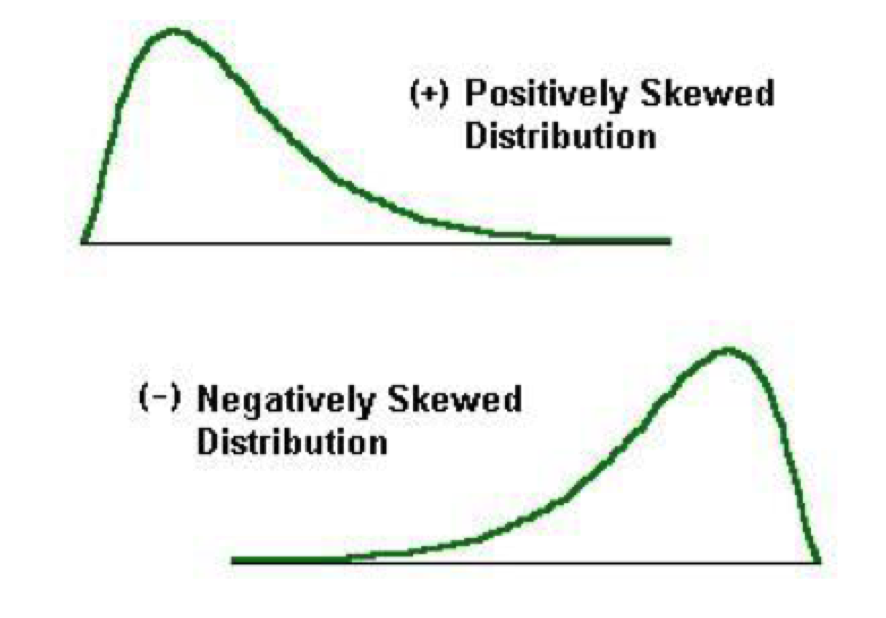
\includegraphics{Notes/Obsidian-Attachments/2-Return-Distributions.png}
\end{itemize}

\hypertarget{kurtosis}{%
\section{Kurtosis}\label{kurtosis}}

Kurtosis measures how concentrated the data is around the mean, or how heavy the tails are. You can only measure kurtosis (meaningfully) if the distribution has 0 skew.

Kurtosis of a distribution is measured against the kurtosis of the Normal distribution, which is \(3\).

\[
Kur = \mathbb{E}\left[ \left( \frac{X-\mu}{\sigma} \right)^{3} \right] - 3
\]
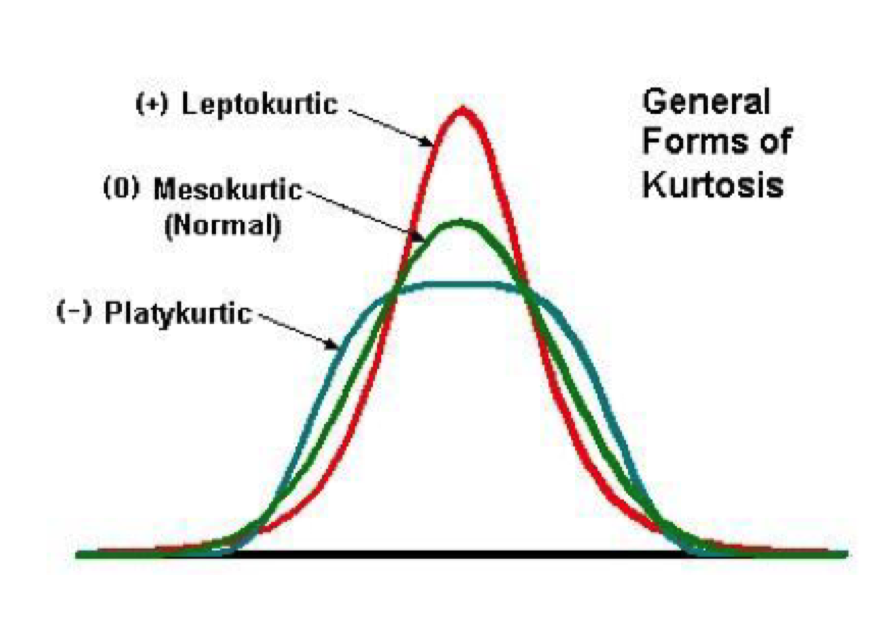
\includegraphics{Notes/Obsidian-Attachments/2-Return-Distributions-1.png}

\hypertarget{qq-plot}{%
\section{QQ Plot}\label{qq-plot}}

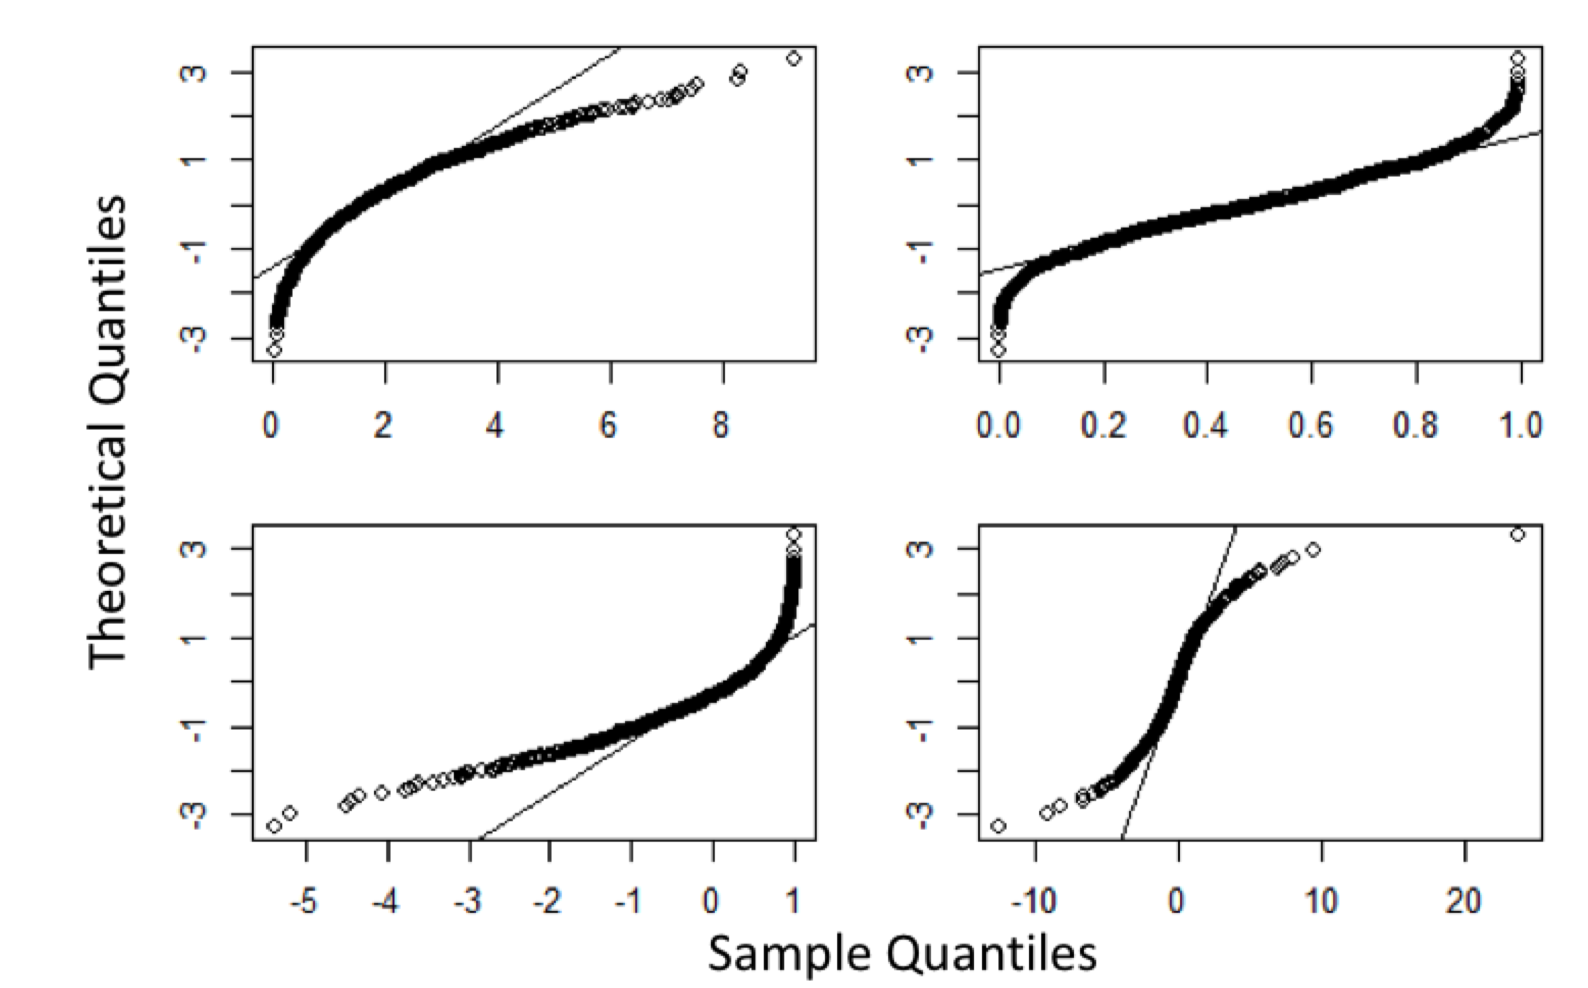
\includegraphics{Notes/Obsidian-Attachments/2-Return-Distributions-2.png}

\begin{itemize}
\tightlist
\item
  Top left: The sample quantiles spread further on the right than the theoretical quantiles, which implies a \textbf{right/pos skewness}
\item
  Top right: The sample quantiles for the tails are very concentrated compared to the theoretical quantiles, which implies the data has short/finite tails implying it is \textbf{platykurtic/neg kurtosis}
\item
  Bottom left: The sample quantiles spread further on the left than the theoretical quantiles, which implies a \textbf{left/neg skewness}
\item
  Bottom right: The sample quantiles for the tails are very spread compared to the theoretical quantiles, which implies the data has long/heavy tails implying it is \textbf{leptokurtic/pos kurtosis}
\end{itemize}

\hypertarget{heavy-tail-distributions}{%
\section{Heavy Tail Distributions}\label{heavy-tail-distributions}}

A distribution \(f(x)\) is said to have:

\begin{itemize}
\tightlist
\item
  Exponential tails (short/finite tails) if
  \[f(x) \propto e^{-x/\lambda}\]
\item
  Polynomial tails (long/heavy tails) if
  \[
  \begin{aligned}
  f(x) &\propto x^{-(1+\alpha)}\\
  \\
  \text{Where } &\alpha \text{ is the tail index}
  \end{aligned}
  \]
\end{itemize}

\begin{quote}
\textbf{The smaller the tail index, the heavier the tail}
\end{quote}

Heavy tailed distributions can also have infinite moments (including the mean!)

\[
\mathbb{E}(X^{k}) = \infty \text{ for } k \geq \alpha
\]
\emph{So if the tail index is high, the tail is lighter, and the first \(\alpha\) moments exist.}

The tail index can be estimated using:
- MLE approximation, which takes the derivative log of the product of n the distributions when it equals 0, and solving for \(\alpha\)
- \(\hat{\alpha} = \frac{n}{\sum^n_{i=1}\ln\left( r_{i}/r_{min} \right)}\)

\[
\begin{aligned}
L(\alpha) &= \prod^{n}_{i=1}[f(x)]\\
\log(L(\alpha)) = l(\alpha) &= \sum^{n}_{i=1} f(x)\\
l'(\alpha) &= \sum^{n}_{i=1} f'(x) = 0
\end{aligned}
\]
- Pareto Q-Q plot of the empirical CDF and the returns in log x log scale
- \(\alpha\) is the estimated slope of the line of best fit

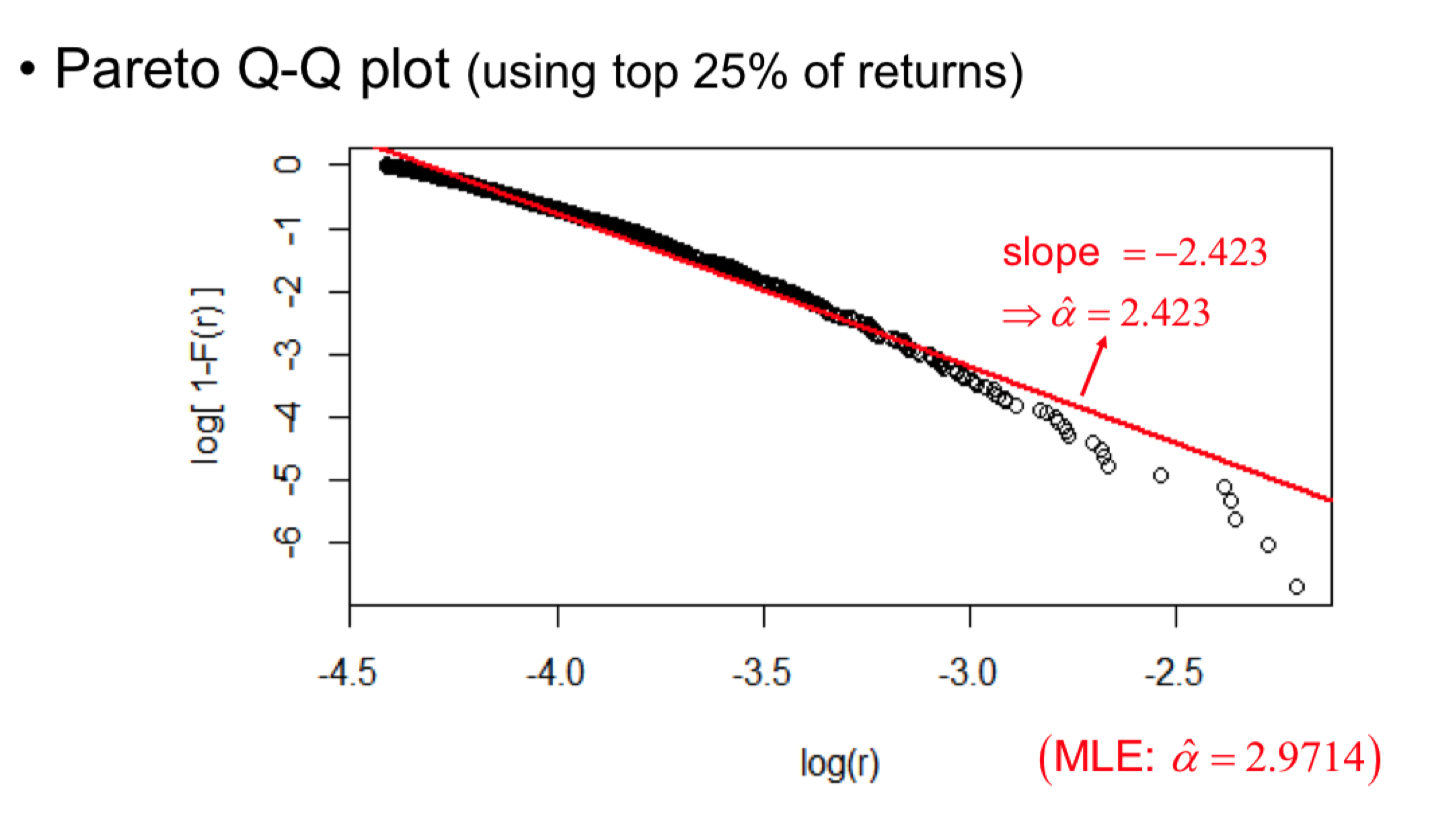
\includegraphics{Notes/Obsidian-Attachments/2-Return-Distributions-3.png}

\hypertarget{common-heavy-tail-distributions}{%
\subsection{Common Heavy Tail Distributions}\label{common-heavy-tail-distributions}}

\hypertarget{pareto}{%
\subsubsection{Pareto}\label{pareto}}

\[
\begin{aligned}
f(x) &= \frac{a\ x^{-(1+\alpha)}}{l^{-\alpha}}, \ x \geq l\\
\end{aligned}
\]

Can be used to model \textbf{absolute} returns above a cutoff \(r_{min}\)
\[
\bar{F}(r) = \left( \frac{r_{min}}{r} \right)^{\alpha} \quad \forall\ r > r_{min}
\]

\hypertarget{standard-cauchy}{%
\subsubsection{Standard Cauchy}\label{standard-cauchy}}

\[
\begin{aligned}
f(x) &= \frac{1}{\pi(1+x^{2})}\\
&= \frac{1+x^{-(\alpha+1)}}{\pi}  \implies \alpha = 1
\end{aligned}
\]
Which is the t-distribution when df = 1.
\[
f(x) \sim t(df=1)
\]

\hypertarget{students-t}{%
\subsubsection{Students t}\label{students-t}}

\[
\begin{aligned}
f(x) &= \frac{\Gamma\left( \frac{v+1}{2} \right)}{\sqrt{ v\pi }\Gamma(v/2)}\left( 1+\frac{x^{2}}{v} \right)^{-\frac{v+1}{2}}\\
\\
\text{Where } &\alpha = v = \text{degrees of freedom}
\end{aligned}
\]
The Students t distributions offers a tractable heavy-tail model of the entire return distribution (not just the tail). It is typically adjusted for the location and scale:

\[
Y = \mu + \sigma X \quad \text{where } X \sim t(df=v)
\]

\hypertarget{stable-distributions}{%
\subsection{Stable Distributions}\label{stable-distributions}}

If we let log returns \(r_{i} \sim\) heavy tail distribution with \(0<\alpha<2\) (the first and second moment - mean/variance exist)

The aggregate return \(r_{1\to n} = r_{1} = r_{2} + \dots r_{n} \sim\) Stable Distribution

\hypertarget{generalized-central-limit-theorem}{%
\subsubsection{Generalized Central Limit Theorem}\label{generalized-central-limit-theorem}}

Stable distributions have no closed form expression, although the share heavy tails and the same tail index \(\alpha\) as it's individual distributions.

As you sum independent, \textbf{STABLE} random variables, the sum will follow a Stable Distribution.

\hypertarget{measuring-tail-behaviour}{%
\subsubsection{Measuring tail behaviour}\label{measuring-tail-behaviour}}

We use the complementary CDF
\[
\bar{F}(x) = 1 - F(x) = P(X > x) \sim x^{-\alpha}
\]

\hypertarget{mixture-distributions}{%
\section{Mixture Distributions}\label{mixture-distributions}}

We can generate a random variable using one of out a selection of a family of distributions, choosing the distribution using another distribution.

They are easy to generate, but harder to work with analytically.

We can select from a discrete and finite set of distributions, or of a continuous family of distributions (possibly countable) known as compound distributions.

Example:
\[
\begin{aligned}
\text{Generate RV from: } \begin{cases}
N(0,1) & p=60\%\\
N(5,3) & p=40\%
\end{cases}
\end{aligned}
\]
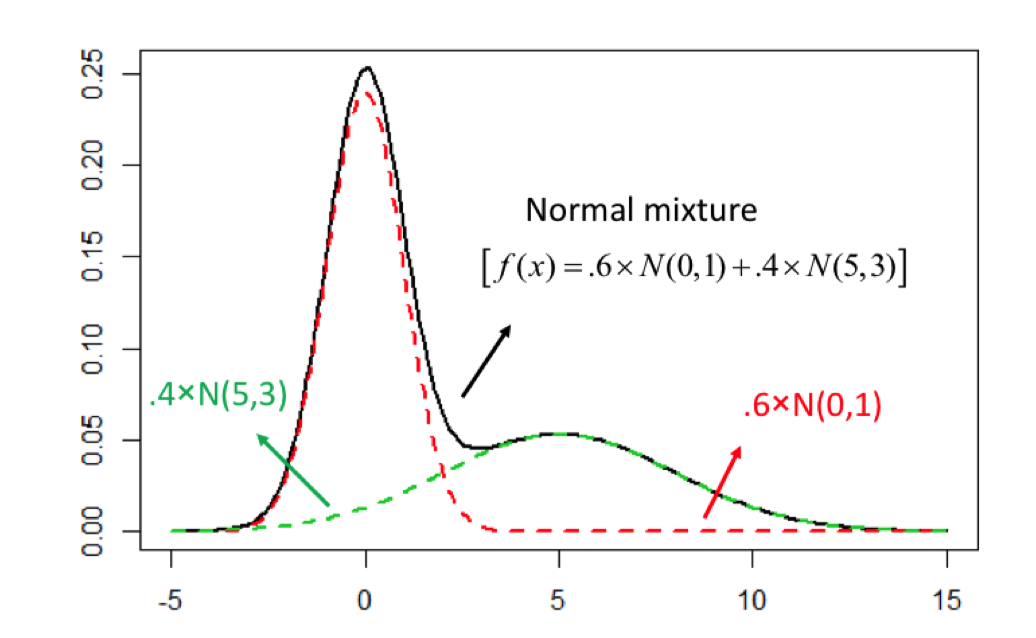
\includegraphics{Notes/Obsidian-Attachments/2-Return-Distributions-4.png}

\hypertarget{normal-scale-mixture}{%
\subsubsection{Normal scale mixture}\label{normal-scale-mixture}}

\(Y = \mu+\sqrt{ V } \cdot Z\)
Where \(V\) is a RV with non-negative mixing distribution and represents a random sd of \(Y\).

Example (probably don't need to memorize\ldots) which is used when simulating returns, as seem in PS2 Q4c part ii and iii.

\[
\begin{aligned}
\text{t-dist } t &= Z\sqrt{ v/W } \quad \text{ where } W \sim \chi^{2}(df=v)\\
\text{GARCH model } r_{t} &= \mu + \sigma_{t}Z_{t} \quad \text{ where } \sigma^{2}_{t} = \omega + \sum^{p}_{i=1}a_{i}r^{2}_{t-i}+\sum^{q}_{j=1}\beta_{j}\sigma^{2}_{t-j}\\
\end{aligned}
\]

\hypertarget{modelling-extreme-events}{%
\chapter{Modelling Extreme Events}\label{modelling-extreme-events}}

\hypertarget{stylized-facts}{%
\section{Stylized Facts}\label{stylized-facts}}

Characteristics of typical empirical asset returns:

\begin{enumerate}
\def\labelenumi{\arabic{enumi}.}
\tightlist
\item
  Absence of simple autocorrelations

  \begin{itemize}
  \tightlist
  \item
    Returns are not correlated with past time-steps of itself
  \end{itemize}
\item
  Volatility clustering

  \begin{itemize}
  \tightlist
  \item
    Large amounts of volatility often occur in clusters through time
  \end{itemize}
\item
  Heavy tails

  \begin{itemize}
  \tightlist
  \item
    Returns often have very abnormal (large) values suggesting heavy tail distributions
  \end{itemize}
\item
  Intermittency
\item
  Aggregation changes distribution
\item
  Gain/loss asymmetry

  \begin{itemize}
  \tightlist
  \item
    The market tends to go up over time
  \end{itemize}
\end{enumerate}

\hypertarget{extreme-value-theory}{%
\section{Extreme Value Theory}\label{extreme-value-theory}}

This theory helps with modelling extreme events that have small probabilities of occurring.

\hypertarget{two-main-results}{%
\subsection{Two main results}\label{two-main-results}}

\begin{itemize}
\tightlist
\item
  Maxima of i.i.d. sequences
\item
  Values exceeding threshold
\end{itemize}

\hypertarget{st-theorem-fisher-tippet-gnedenko}{%
\subsection{1st Theorem: Fisher-Tippet-Gnedenko}\label{st-theorem-fisher-tippet-gnedenko}}

\emph{Theres no need to prove any results}

If \(X_{1}, X_{2}, \dots\) are i.i.d. RVs, we can create a RV that simply takes the maximum of \(n\) RVs called \(M_{n} = max(X_{1}, X_{2}, \dots X_{n})\).

\textbf{In certain cases}, we can find normalizing constants \(a_{n}>0, b_{n}\) such that they can be transformed into one of the three distributions (identified by \(H(x)\)) which can be much easier to work with.

\[
\begin{aligned}
P\left( \frac{M_{n}-b_{n}}{a_{n}} \leq x\right) &= [F(a_{n}x+b_{n})]^{n} \to H(x)\\
F(a_{n}x+b_{n}) &= \text{Single RV}
\end{aligned}
\]
This is just saying that the normalized max RV is less than some value \(x\) is just the probability of each individual RV being less than the transformed value of \(x\).

\[
\begin{aligned}
H(x) &= \begin{cases}
Gumbel & \exp\{-e^{-x}\} \quad\quad x \in \mathbb{R}\\
Frechet & \begin{cases}
0 & x < 0 \\
\exp\{-x^{-\alpha}\}  & x >0
\end{cases}\\
Weibull  & \begin{cases}
\exp\{-|x|^{\alpha}\}  & x<0 \\
1 & x > 0
\end{cases}
\end{cases}
\end{aligned}
\]
Where \(\alpha > 0\) for the Frechet and Weibull distributions.

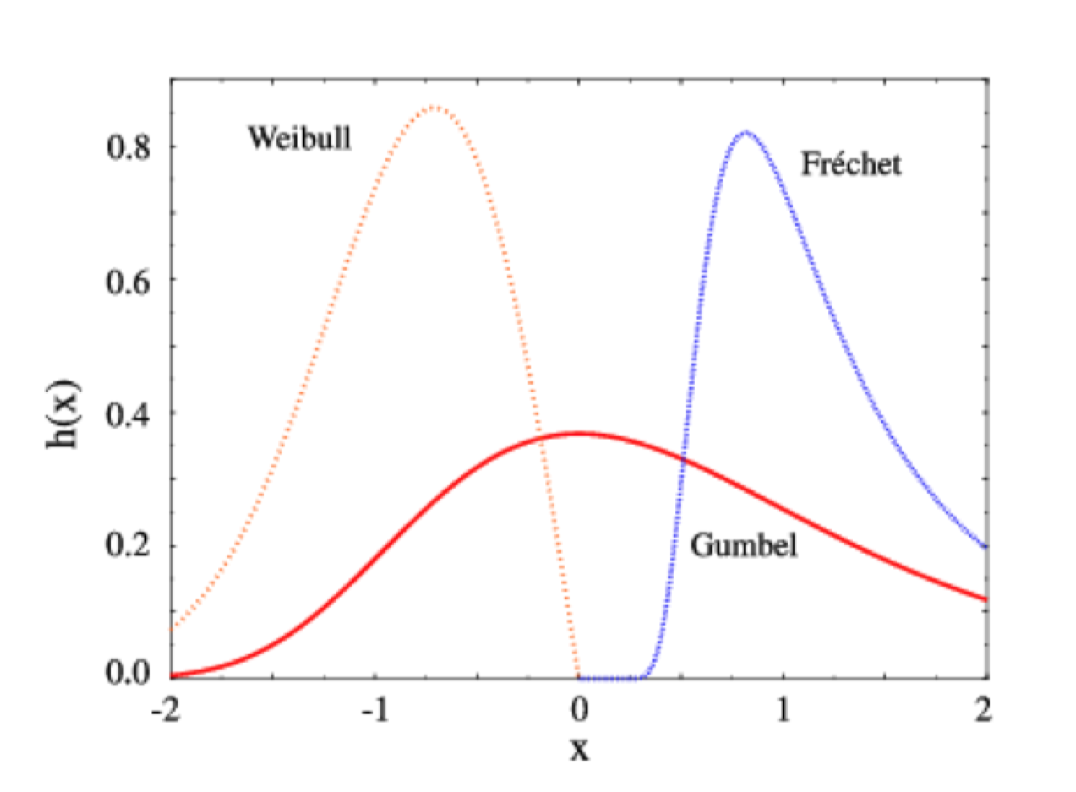
\includegraphics{Notes/Obsidian-Attachments/3-Modelling-Extreme-Events.png}

\hypertarget{generalized-extreme-value-gev-distribution}{%
\subsection{Generalized Extreme Value (GEV) Distribution}\label{generalized-extreme-value-gev-distribution}}

The three types of distributions can be represented using:
\[
\begin{aligned}
H(x) &= \exp\left\{ -\left( 1+\xi\frac{x-\mu}{\sigma} \right)^{-1/\xi}_{+} \right\}\\
\text{Where } \mu &= \text{location}\\
\sigma &= \text{scale}\\
\xi &= \text{shape parameters} \begin{cases}
\xi>0 & \text{heavy tails (Frechet)} \\
\xi=0 & \text{exponential tails (Gumbel)} \\
\xi < 0  & \text{short/light tails (Weibull)}
\end{cases}
\end{aligned}
\]
Where the \(\xi\) value describes the tail behaviour

The log-transformation of the Frechet(\(\alpha=1\)) is the Gumbel distribution!
\[
\begin{aligned}
\ln(H_{F}(x)) &= \ln\left[ \exp\{-x^{-1}\}\right]\\
&= -\left( 1+\frac{x-\mu}{\sigma} \right)^{-1}\\
\\
&= H_{G} = \exp \left\{ -\left( 1+0\cdot \frac{x-\mu}{\sigma} \right)^{-1/0} \right\}
\end{aligned}
\]

As an example, we'll show that the normalized maximum of i.i.d. Uniform(0,1) aka \(F_{n}(x) = x\) with \(a_{n}=1/n, b_{n}=1\) converges to the Weibull distribution.
\[
\begin{aligned}
P\left( \frac{M_{n}-b_{n}}{a_{n}} \leq x\right) &= P\left( \frac{M_{n}-1}{1/n} \leq x\right)\\
& b_{n}\text{ shifts the Uniform from (0,1) to (-1,0)}\\
&= P\left( M_{n} \leq \frac{x}{n}+1 \right)\\
&= P\left( \max(U_{1}, U_{2}, \dots U_{n}) \leq 1+\frac{x}{n} \right)\\
&= \prod^{n}_{i=1} \underbrace{ P\left( U_{i}\leq 1+\frac{x}{n} \right) }_{ \left( 1+\frac{x}{n} \right) }\\
&= \left( 1+\frac{x}{n} \right)^{n}\\
& \text{because } x<0, \quad 1+ (-.4) = 1-|-.4|\\
&=\left( 1-\frac{|x|}{n} \right)^{n}\\
\\
\lim_{ n \to \infty } \left( 1-\frac{|x|}{n} \right)^{n} &\to \exp\{((-1)|x|)^{-1/-1}\}\\
&= \exp\{-|x|^{1}\} \implies Weibull(\alpha=1)\\
\end{aligned}
\]

\hypertarget{nd-theorem-pickands-balkema-de-haan}{%
\subsection{2nd Theorem: Pickands-Balkema-De Haan}\label{nd-theorem-pickands-balkema-de-haan}}

For any RV \(X\) with CDF \(F(\cdot)\), it's conditional distribution when exceeding a certain threshold \(u\) is:
\[
\begin{aligned}
F_{u}(y) &= \frac{F(u+y)-F(u)}{1-F(u)}, \quad 0\leq y\leq x_{F}-u\\
\text{Where } x_{F} &= sup\{x \in \mathbb{R}:F(x) < 1\} \text{ is the right endpoint of } F
\end{aligned}
\]

\(x_{F}\) could be finite, or \(\infty\). As \(u\to x_{F}\), the conditional distribution converges to something belonging to the \textbf{Generalized Pareto Distribution (GPD).}
\[
F_{u}(y) \to G_{\xi, \sigma}(y)
\]
The \textbf{Generalized Pareto Distribution (GPD)} is given by:
\[
\begin{aligned}
G_{\xi,\sigma}(y) &= 1 - \left( 1+\xi \frac{y}{\sigma} \right)^{-1/\xi}_{+} = \begin{cases}
G_{\xi, \sigma}(y) = 1-\left( 1+\xi  \frac{y}{\sigma} \right)^{-1/\xi}  & \xi \ne 0\\
G_{\xi, \sigma}(y) = 1-\exp\left\{ -\frac{y}{\sigma} \right\}  & \xi = 0
\end{cases}\\
\text{Where } & \sigma > 0, y\geq 0, \quad y\leq-\frac{\sigma}{\xi} \text{ when } \xi < 0
\end{aligned}
\]

\(f(x) = \lambda e^{-\lambda x}, \lambda>0\)

\begin{Shaded}
\begin{Highlighting}[]
\NormalTok{bottom={-}1; left={-}0.5; right=1.5;}
\NormalTok{{-}{-}{-}}
\NormalTok{y=2 \textbackslash{}exp({-}2x)}
\NormalTok{x=.9|dashed}
\end{Highlighting}
\end{Shaded}

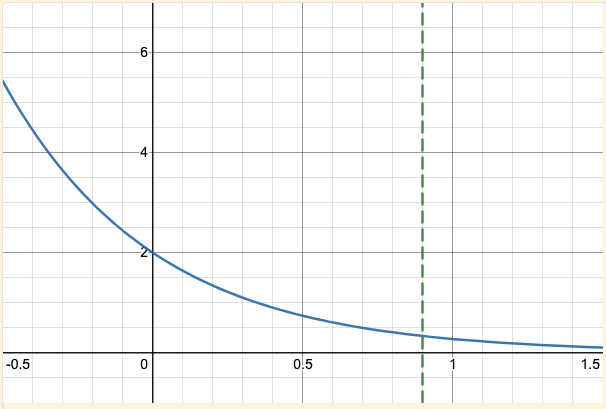
\includegraphics{Notes/Obsidian-Attachments/3-Modelling-Extreme-Events-1.png}

The exponential distribution is used to model waiting times, no matter how much time has passed. The conditional distribution

\hypertarget{multivariate-return-modelling}{%
\chapter{Multivariate Return Modelling}\label{multivariate-return-modelling}}

When modelling returns of multiple assets, it's common to assume the correlation between them is constant.

Many investment strategies combine multiple assets together, but how those assets are related is an important piece of information to understand. It's also difficult to model. Say we start with a simple multivariate Normal, where dependence \(\leftrightarrow\) covariance, so we can model their relations with the covariance matrix.

\hypertarget{covariance-correlation-matrix}{%
\section{Covariance \& Correlation Matrix}\label{covariance-correlation-matrix}}

For a linear combination of assets, we can attempt to use the following covariance matrix to describe their linear dependence:
\[
\begin{aligned}
Cov[A^{T}R] = A^{T}Cov[R]A, \quad \text{where }\begin{cases}
A = \text{Constant matrix} \\
R = \text{random vector}
\end{cases}
\end{aligned}
\]
Unfortunately, sample covariance estimation is very sensitive to extreme values, which happen frequently with return (See heavy tails)

Returns are often treated as independent samples, but that is not realistic.

\hypertarget{multivariate-students-t-distribution}{%
\section{Multivariate Student's t Distribution}\label{multivariate-students-t-distribution}}

We should \textbf{never remove outliers} in finance. We must model the heavy tails (extreme returns) somehow, and Student's t distribution is one way to do that.

A multivariate Normal scale mixture model can be used to describe a multivariate Student's t distribution:
\[
\begin{aligned}
\mathbf{R} &= \boldsymbol{\mu} + \mathbf{Z} \sqrt{ v/W } \sim t_{v}(\boldsymbol{\mu}, \boldsymbol{\Lambda})\\
\\
\text{Where } & W \sim \chi^{2}(df=v)\\
& \mathbf{Z} \sim N(\mathbf{0}, \boldsymbol{\Lambda}) \quad \text{where } \boldsymbol{\Lambda} = Indentity \ Mat
\end{aligned}
\]

It's mean and variance are:

\[
\begin{aligned}
\mathbb{E}(\mathbf{R}) &= \mathbb{E}\left( \boldsymbol{\mu}+\mathbf{Z}\sqrt{ \frac{v}{W} }\right)\\ 
&= \boldsymbol{\mu} + \underbrace{ \mathbb{E}(\mathbf{Z}) }_{ =0 }\cdot \mathbb{E}\left( \sqrt{ \frac{v}{W} } \right)\\
&=\boldsymbol{\mu}\\
\\
Cov(\mathbf{R}) &= Cov\left( \boldsymbol{\mu} + \mathbf{Z} \sqrt{ \frac{v}{W} } \right)\\
&= Cov(\mathbf{Z}) \cdot Cov\left( \sqrt{ \frac{v}{W} } \right)\\
&= \boldsymbol{\Lambda}\cdot \frac{v}{v-2} \quad \text{where } v > 2
\end{aligned}
\]

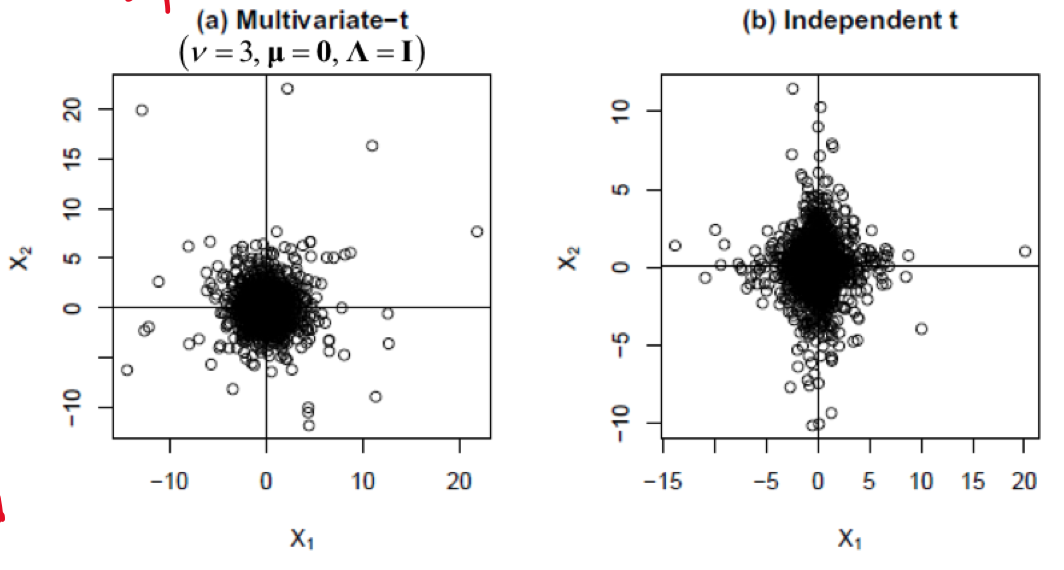
\includegraphics{Notes/Obsidian-Attachments/4-Multivariate-Return-Modelling.png}

From these plots, we see that with the Multivariate t distribution, the extreme values between the two RVs are more evenly spread (the round shape of the points) and imply extreme values for both assets happen together. This is because they both share the same \(\Lambda\).

This shows that the multivariate t distribution is more practical and realistic than using the Normal to model multiple assets. We can linearly combine multivariate t-distributions with the same degrees of freedom:

\[
\begin{aligned}
\mathbf{Y} &\sim t_{v}(\boldsymbol{\mu}, \boldsymbol{\Lambda}) \implies \mathbf{w}^{T}\mathbf{Y} \sim t_{v}(\mathbf{w}^{T}\boldsymbol{\mu}, \mathbf{w}^{T}\boldsymbol{\Lambda}\mathbf{w})\\
\\
\mathbb{E}[\mathbf{w}^{T}\mathbf{Y}] &= \mathbf{w}^{T}\mathbb{E}(\mathbf{Y})\\
Var[\mathbf{w}^{T}\mathbf{Y}] &= \mathbf{w}^{T}Var\left( \boldsymbol{\mu}+\mathbf{Z}\sqrt{ \frac{v}{W} } \right)\mathbf{w}\\
&= \mathbf{w}^{T}Var(\mathbf{Z})Var\left( \sqrt{ \frac{v}{W} } \right)\mathbf{w}\\
&= \frac{v}{v-2}(\mathbf{w}^{T}\boldsymbol{\Lambda}\mathbf{w})
\end{aligned}
\]

However, as seen above, the multivariate t distribution is \textbf{restrictive} because all the marginal distributions share the same degrees of freedom, as they all depend on the variance of \(W \sim\chi^{2}\).

\hypertarget{copulas}{%
\chapter{Copulas}\label{copulas}}

A more flexible way of modelling dependencies of RVs is using copulas.

\begin{quote}
Definition: A copula (C) is a multivariate CDF with Uniform(0,1) marginals
\end{quote}

\[
\begin{aligned}
C(u_{1}, u_{2}, \dots u_{d}) &=P(u_{1}, u_{2}, \dots u_{d}) \in [0,1], \quad \forall \ u_{1},\dots u_{d} \in [0,1]\\ 
\\
&\text{Where }\begin{cases}
C(0,0, \ldots, 0)=0 \\
C(1,1, \ldots, 1)=1 \\
C\left(\ldots, u_{i-1}, 0, u_{i+1}, \ldots\right)=0 \\
C\left(1, \ldots, 1, u_i, 1, \ldots, 1\right)=u_i
\end{cases}
\end{aligned}
\]
Third case: The cumulative probability of one RV being less than or equal to 0 regardless of what the other RVs are in a copula is 0.
Fourth case: The cumulative probability that the other RVs have values less than 1 is 1 but the \(i^{th}\) RV is \(u_{i}\) is simply \(u_{i}\)

\hypertarget{the-independence-copula}{%
\section{The independence copula}\label{the-independence-copula}}

\begin{quote}
\textbf{Definition:} \(C_{indep} (u_{1}, \dots u_{d}) = u_{1} \times \dots \times u_{d}\)
\end{quote}

By the \textbf{Frechet-Hoeffding} theorem, any/every copula is bounded by

\[
\begin{aligned}
& \underline{C}\left(u_1, \ldots, u_d\right) \leq C\left(u_1, \ldots, u_d\right) \leq \bar{C}\left(u_1, \ldots, u_d\right) \\
& \text { where }
\begin{cases}
\underline{C}\left(u_1, \ldots, u_d\right)=\max \left\{1-d+\sum_{i=1}^d u_i, 0\right\} = \max\left\{ 1 - \left(\sum^d_{i=1} 1 - u_{i}\right),0 \right\} \\
\bar{C}\left(u_1, \ldots, u_d\right)=\min \left\{u_1, \ldots, u_d\right\}
\end{cases}
\end{aligned}
\]
\(\max \left\{1-d+\sum_{i=1}^d u_i, 0\right\}\) is 1 minus number of uniforms plus the values of the uniforms

\begin{itemize}
\tightlist
\item
  (if \(\mathbf{d=5}, u_{1}=.5,u_{2}=.4,u_{3}=.7,u_{4}=.2,u_{5}=.6\)

  \begin{itemize}
  \tightlist
  \item
    then \(\max(1-5+2.4 = \mathbf{-1.6},0)\) )
  \end{itemize}
\item
  This implies the maximum of the Copula is bounded by 0, or higher if the average value of the uniforms are \(\geq\frac{d-1}{d}\).
\end{itemize}

\(\min \left\{u_1, \ldots, u_d\right\}\) implies the max of the Copula is bounded by the smallest marginal probability, which makes sense as that is the only one limiting the \textbf{cumulative probability}.

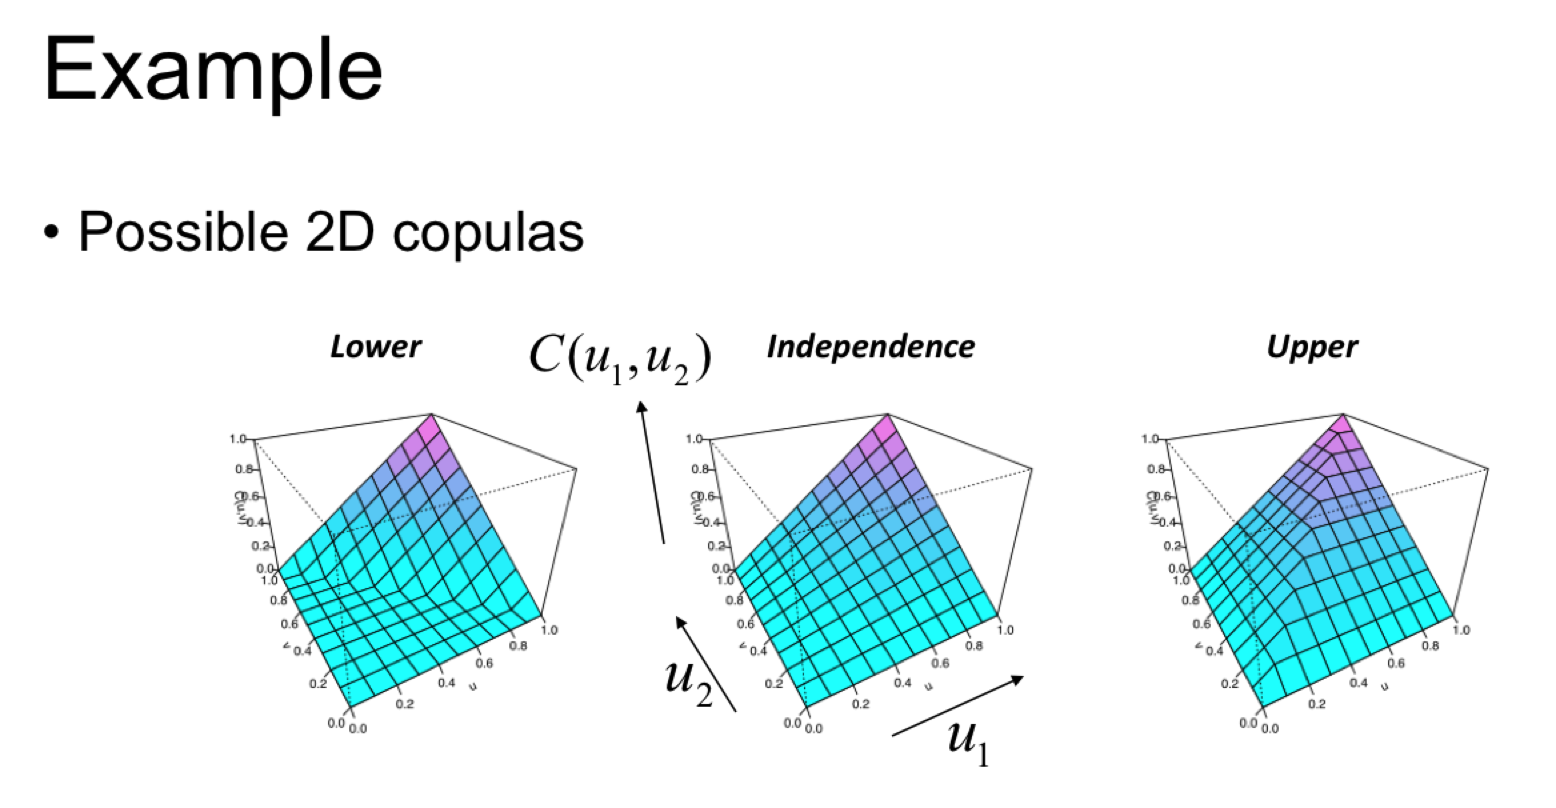
\includegraphics{Notes/Obsidian-Attachments/4-Multivariate-Return-Modelling-1.png}

\hypertarget{sklars-theorem}{%
\section{Sklar's Theorem}\label{sklars-theorem}}

Any continuous multivariate CDF \(F(x_{1}, \dots x_{d})\) with marginal (1D) CDF's \(F_{i}(x_{i}) \ \forall \ i=1,\dots,d\) can be expressed in terms of a copula \(C\), as
\[
F(x_{1},\dots x_{d}) = C(F_{1}(x_{1}), \dots, F_{d}(x_{d}))
\]

Inverse is also true, where any copula combined with marginal CDF's can give a multivariate CDF.

\begin{itemize}
\tightlist
\item
  Copula's model dependence separately from the marginal distributions of the RVs
\end{itemize}

If \(X \sim F \implies F(x) \sim Unif(0,1) \implies F^{-1}(Unif) \sim F\)
\emph{If an RV follows some CDF \(F\), then \ldots{}}

\begin{quote}
If you take a copula of a bunch of marginal CDF's, you can obtain the multivariate CDF of all the marginals. The inverse is true, where you can take a multivariate CDF and come up with a copula to represent the dependency between the marginal distributions, and the marginal distributions themselves. (I think is what this is saying.)
\end{quote}

\hypertarget{example}{%
\subsection{Example}\label{example}}

For a continuous CDF \(F(x_{1},\dots,x_{d})\) with marginals \(F_{i}(x_{i})\), the copula is given by:
\[
\begin{aligned}
C(F_{1}(x_{1}),\dots,F_{d}(F_{d})) &= F(x_{1},\dots,x_{d}) \ \text{by Sklar's Thm}\\
\\
\text{Let } u_{i}= F_{i}(x_{i}) &\implies x_{i} = F_{i}^{-1}(u_{i})\\
\end{aligned}
\]
\[
\therefore \mathbf{C(u_{1},\dots,u_{d}) = F(F_{1}^{-1}(u_{1}),\dots,F_{d}^{-1}(u_{d}))}\\
\]

\hypertarget{gaussian-copula}{%
\section{Gaussian Copula}\label{gaussian-copula}}

We can also construct copula's of non uniform distributions, such as this multivariate Normal CDF:

\[
\text{Let } \mathbf{X}\sim N_{d}(\boldsymbol{\mu}, \boldsymbol{\Sigma}) \quad \text{with Correlation Mat} \ \boldsymbol{\rho}\\
\]
We can find the copula \(C_{p}\) of \(\mathbf{X}\) using:
\[
C_{p}(u_{1},\dots u_{d}) = \Phi_{\boldsymbol{\mu},\boldsymbol{\Sigma}}(\Phi_{\mu_{1},\sigma_{1}^{2}}^{-1}(u_{1}), \dots, \Phi_{u_{d},\sigma_{d}^{2}}^{-1}(u_{d}))
\]
For multivariate distributions that have a Gaussian Copula are called \textbf{meta-Gaussian} distributions. These distributions themselves do not need to be Gaussian.

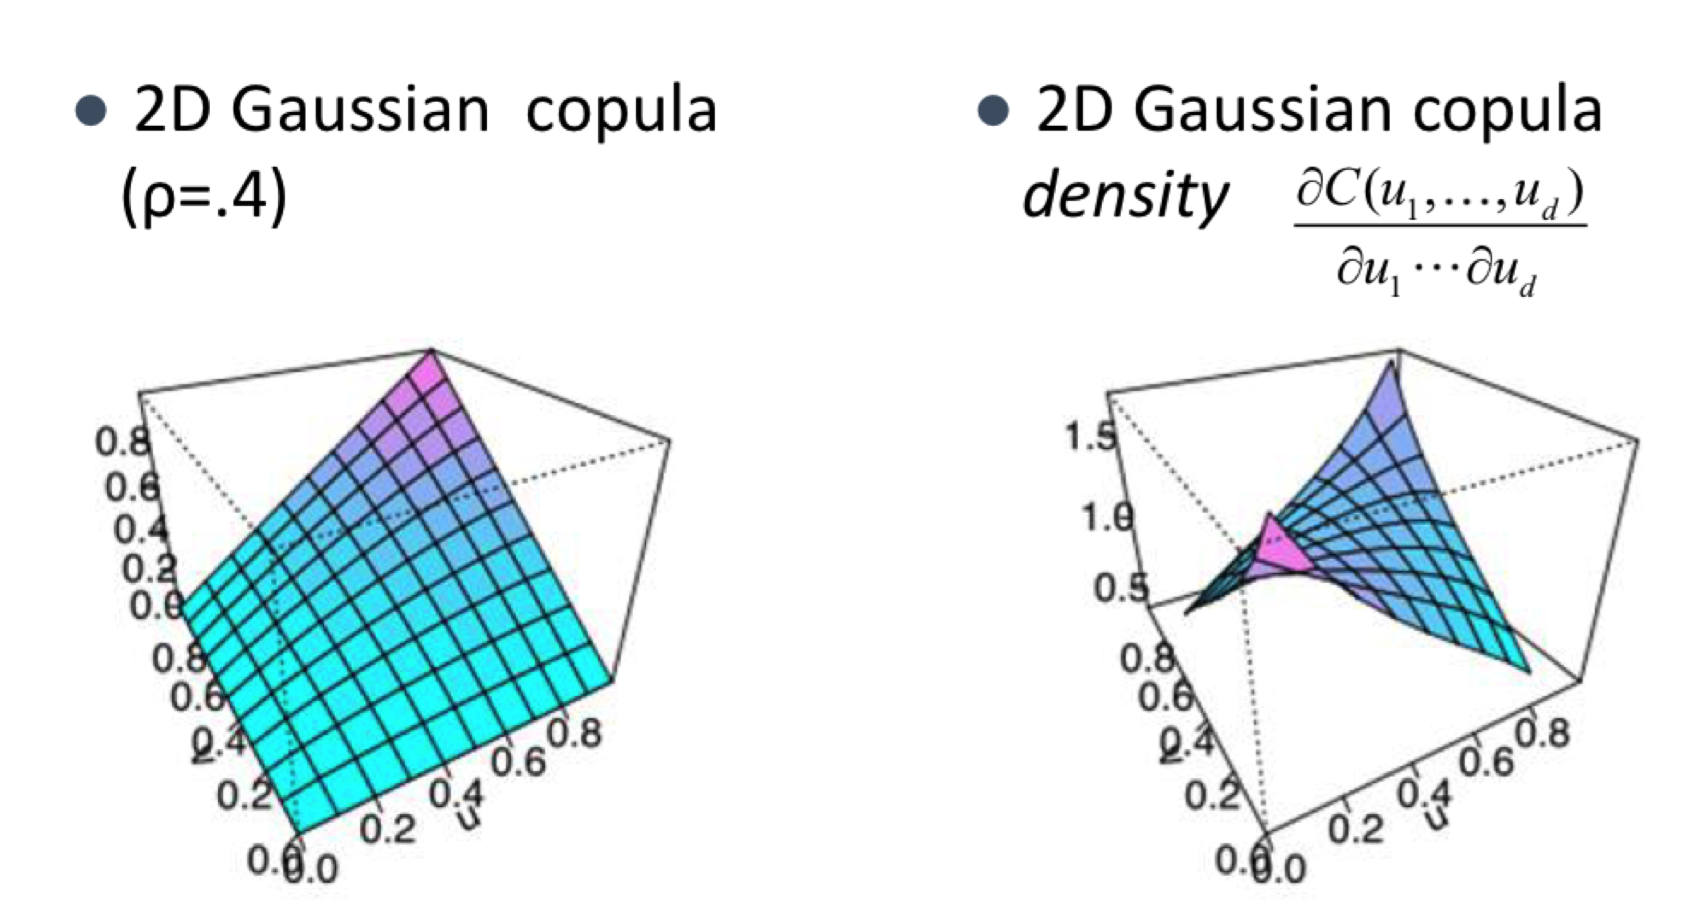
\includegraphics{Notes/Obsidian-Attachments/4-Multivariate-Return-Modelling-2.png}

The second plot would be flat/uniform if the two independent distributions were not correlated (\(\rho=0\)). This plot shows that the probability of both being \(1\) or \(0\) is very high, but the probability that one is \(1\) and the other is \(0\) is virtually 0. This supports our goal of modelling distributions where extreme values occur together.

\hypertarget{creating-copulas-from-multivariate-distributions}{%
\section{Creating Copula's from Multivariate Distributions}\label{creating-copulas-from-multivariate-distributions}}

We can create Copula's from known multivariate Distributions such as the Normal or t distributions.

\emph{We copy the dependence structure of known distributions (allowing us to use different marginals for modelling)}

\textbf{Copula from multivariate Normal CDF with correlation matrix \(\boldsymbol{\rho}\)}
\[
\begin{aligned}
C_{\rho}(u_{1},\dots ,u_{d}) &= \Phi_{\boldsymbol{\rho}}(\Phi ^{-1}(u_{1}), \dots, \Phi ^{-1}(u_{d}))\\
\end{aligned}
\]
\[
\begin{aligned}
\text{Where } & \begin{cases}
\Phi_{\rho} \text{ is multivariate Normal CDF with correlation } \boldsymbol{\rho} \\ \\
\Phi \text{ is Standard univariate Normal CDF}
\end{cases}
\end{aligned}
\]
\#\# Simulating from a Copula
Simulating from a distribution with a copula (dependence between marginals) and marginals themselves can be done with the following steps:

\begin{enumerate}
\def\labelenumi{\arabic{enumi}.}
\tightlist
\item
  Generate (dependent) uniforms from the copula:

  \begin{itemize}
  \tightlist
  \item
    \[
    (U_{1},\dots U_{d}) \sim C
    \]
  \item
    This is done by generating from a multivariate normal with correlation \(\boldsymbol{\rho}\)
    \[
    \mathbf{Z} = \left[ \begin{array}{l}
    Z_{1} \\
    \vdots \\
    Z_{d}
    \end{array} \right] \sim N_{d}(0,\boldsymbol{\rho})
    \]
  \item
    Calculate uniforms as their marginal CDF's (value of uniform var is a probability \(P(Z \leq Z_{i})\))
  \item
    \[
    U_{i}=\Phi(Z_{i}), \ i=1,\dots,d
    \]
  \item
    Then we can use the uniforms with any other marginal
  \item
    This is a very involved process, that we don't need to go into
  \end{itemize}
\item
  Generate target variates from marginals, using the inverse CDF method

  \begin{itemize}
  \tightlist
  \item
    \[
    X_{i} = F_{i}^{-1}(U_{i}) \ \forall \ i
    \]
  \end{itemize}
\end{enumerate}

It's difficult for simulating uniforms from multivariate copula.

Simulating from just the 2D Multivariate normal with a correlation of 75\% compared to simulating from the Gaussian Copula with the same correlation between variables.

\hypertarget{copula-example-plots}{%
\subsection{Copula example plots}\label{copula-example-plots}}

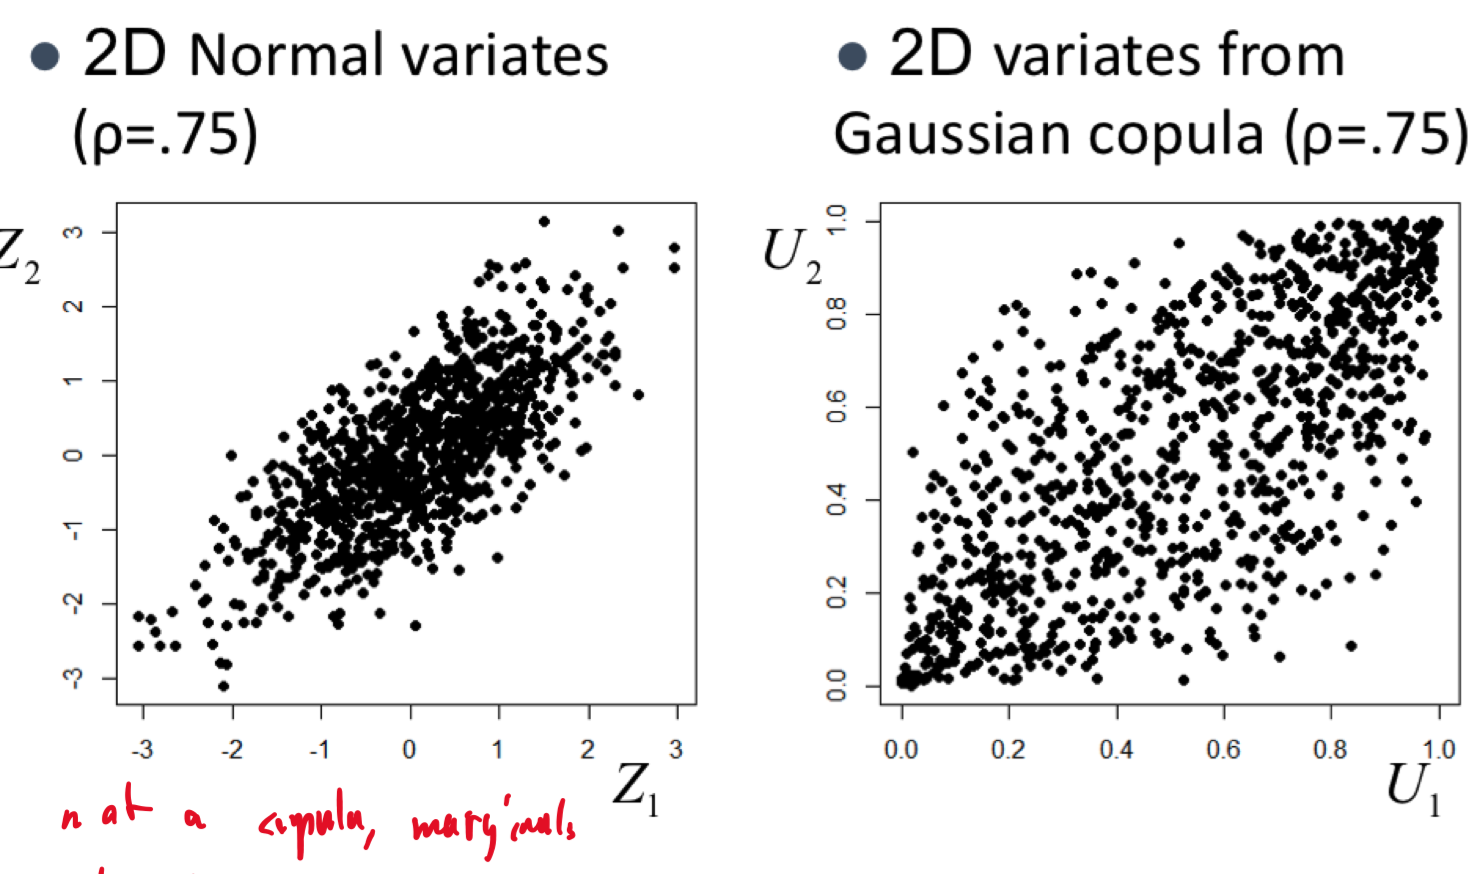
\includegraphics{Notes/Obsidian-Attachments/4-Multivariate-Return-Modelling-3.png}

We can use two different marginals (\(\chi^{2}\) in this case), which are meta-Gaussian as they have a gaussian copula.

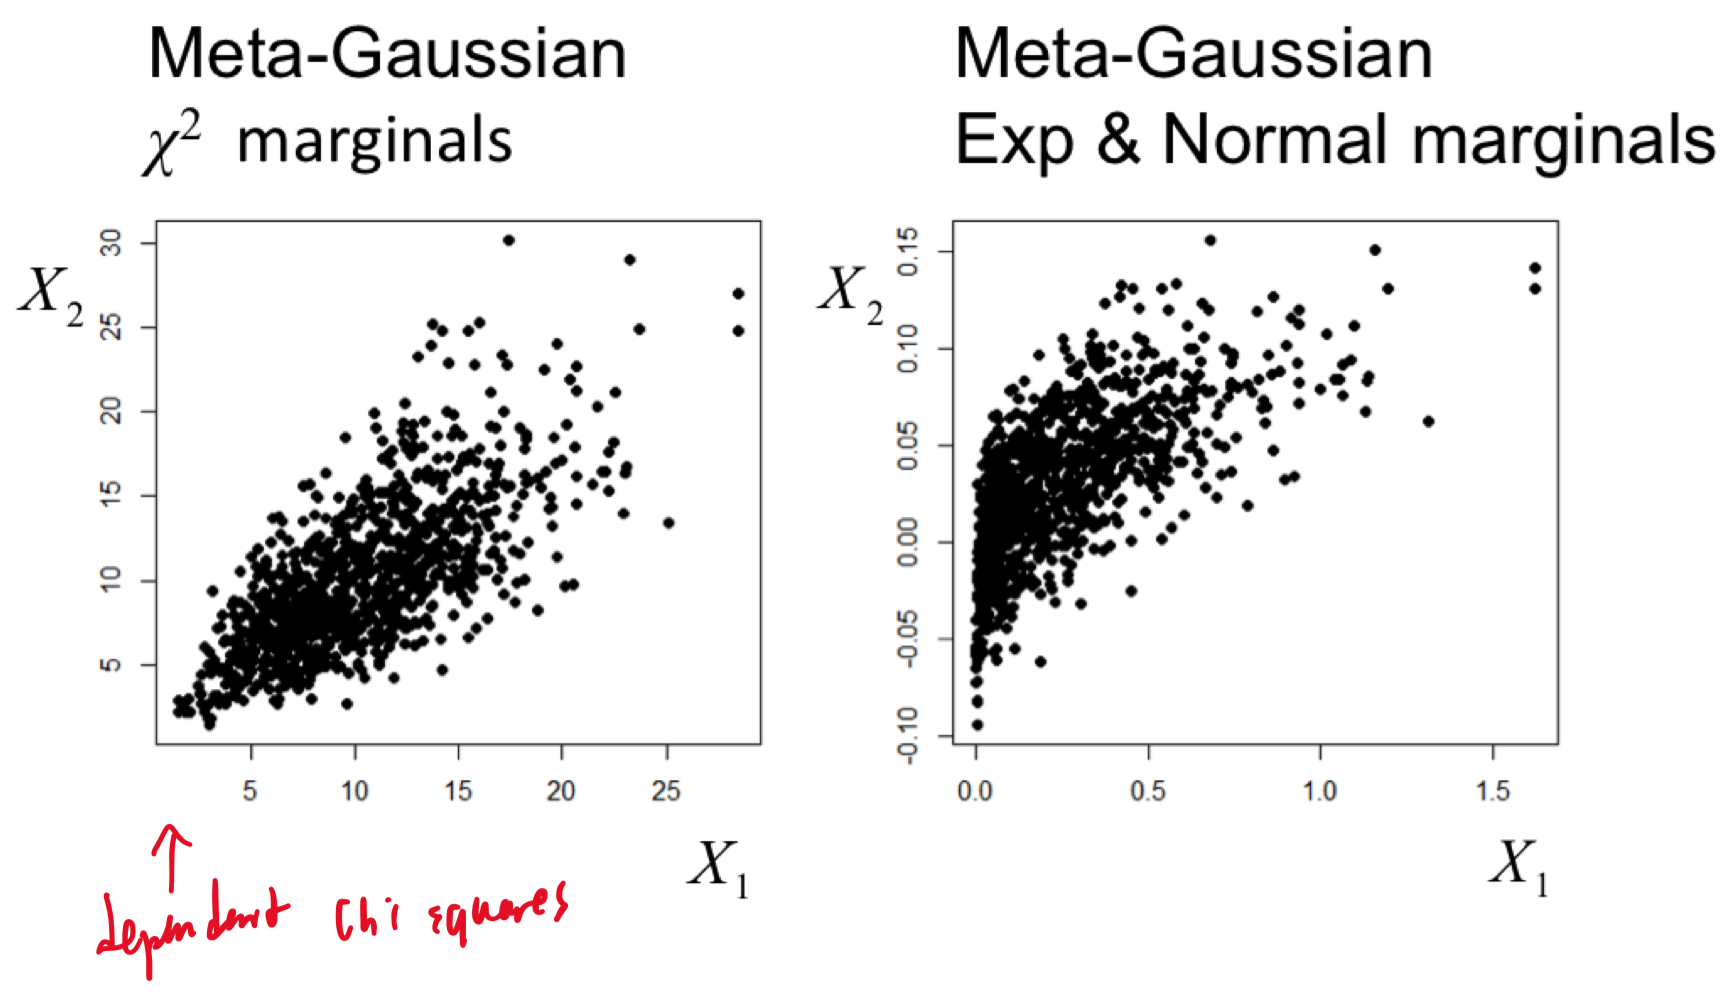
\includegraphics{Notes/Obsidian-Attachments/4-Multivariate-Return-Modelling-4.png}

\begin{quote}
Here we see the simulated copula values for different correlation values.
\end{quote}

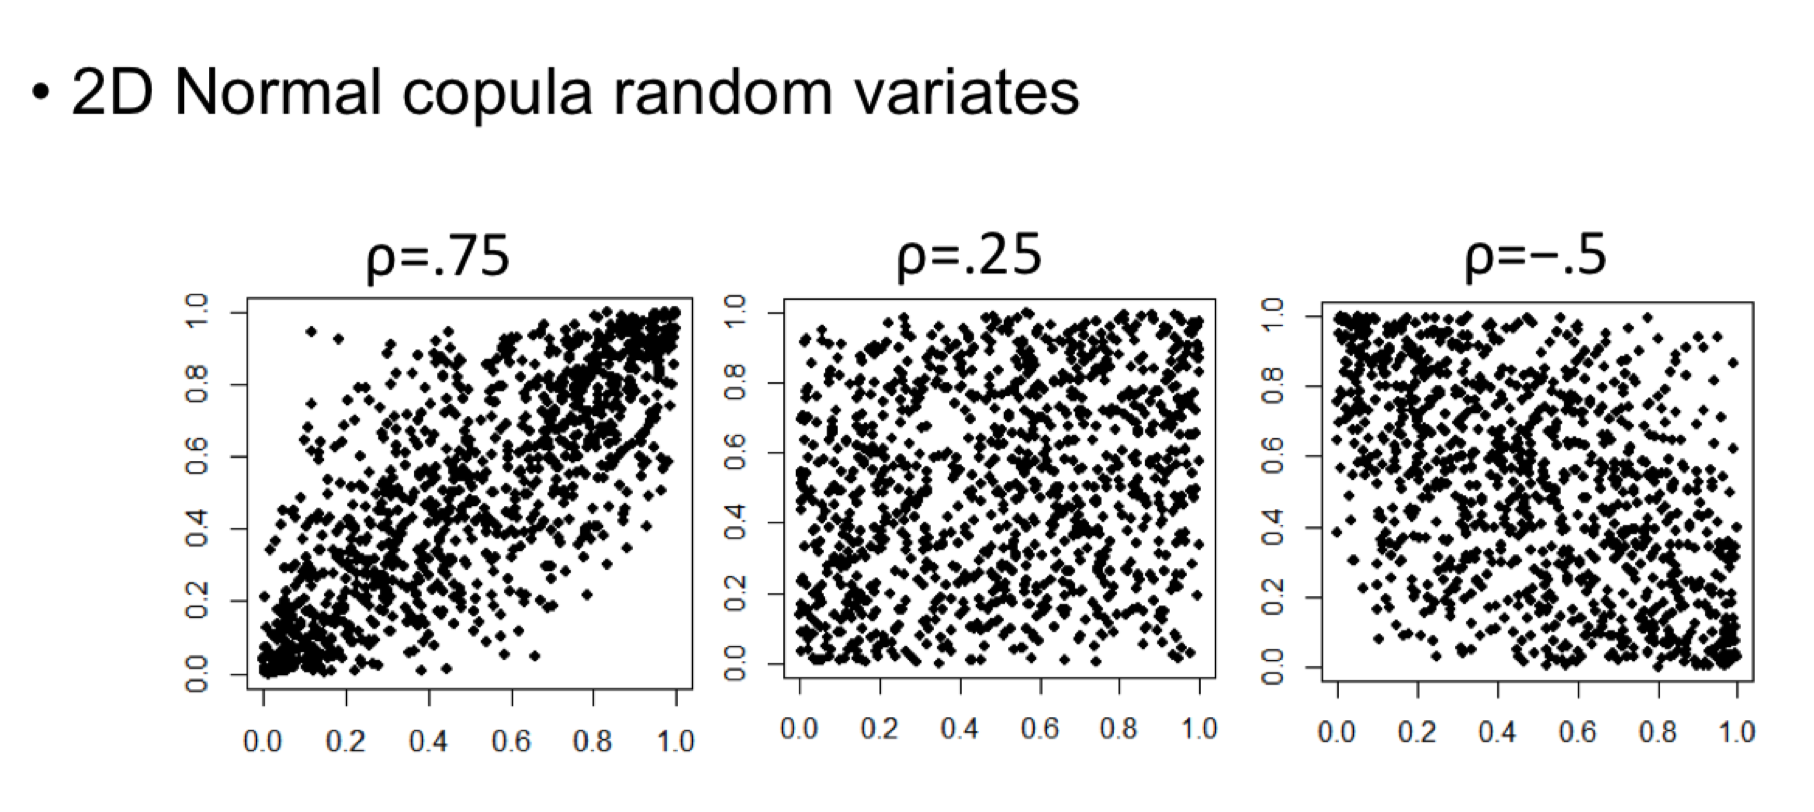
\includegraphics{Notes/Obsidian-Attachments/4-Multivariate-Return-Modelling-5.png}

\begin{quote}
We can also see the differences between a Copula created using Normal and t distributions
\end{quote}

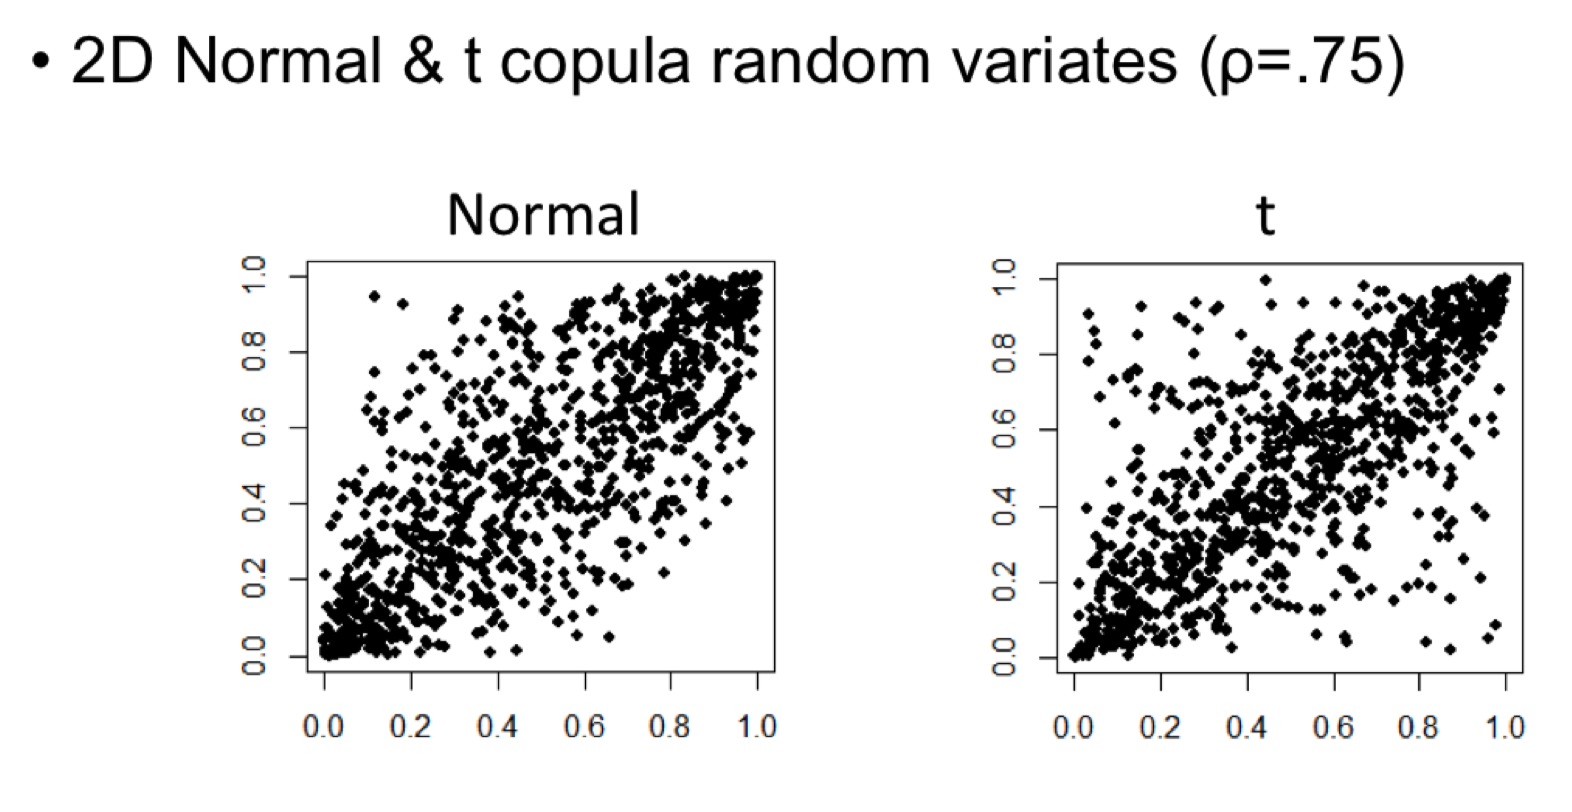
\includegraphics{Notes/Obsidian-Attachments/4-Multivariate-Return-Modelling-6.png}

\begin{quote}
The Normal copula shows \(u_{1},u_{2}\) are independent with 0 correlation as there is equal probability any value is sampled from \(u_{1}\) and any value of \(u_{2}\).

On the right, the t copula shows that values on the borders (\(u_{1}=0 \mid\mid u_{2} =0\)) drop to probability 0, and at the extreme values, jump very high.

Peaks at extreme combinations \(\to\) manifestation of tail dependence.
\end{quote}

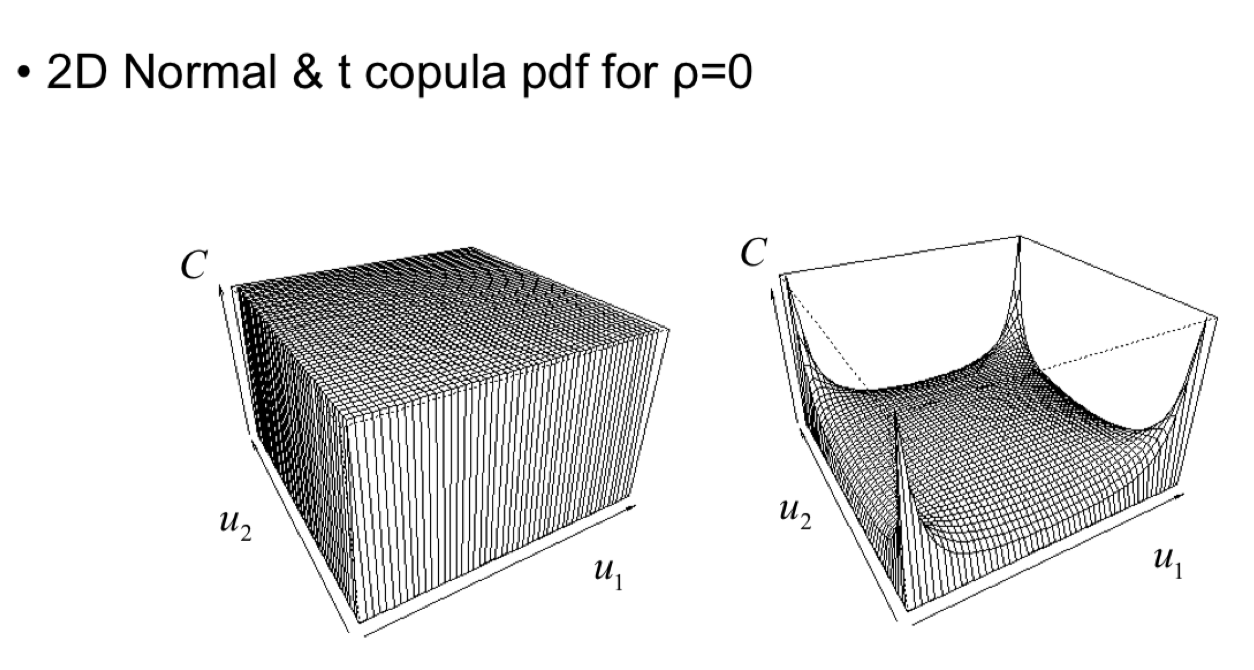
\includegraphics{Notes/Obsidian-Attachments/4-Multivariate-Return-Modelling-7.png}

\hypertarget{elliptical-copulas}{%
\section{Elliptical Copulas}\label{elliptical-copulas}}

The Normal and t distributions have a specific type of dependence: \textbf{elliptical dependence}.

The ellipses describe the contours of the multivariate Normal and t distributions:

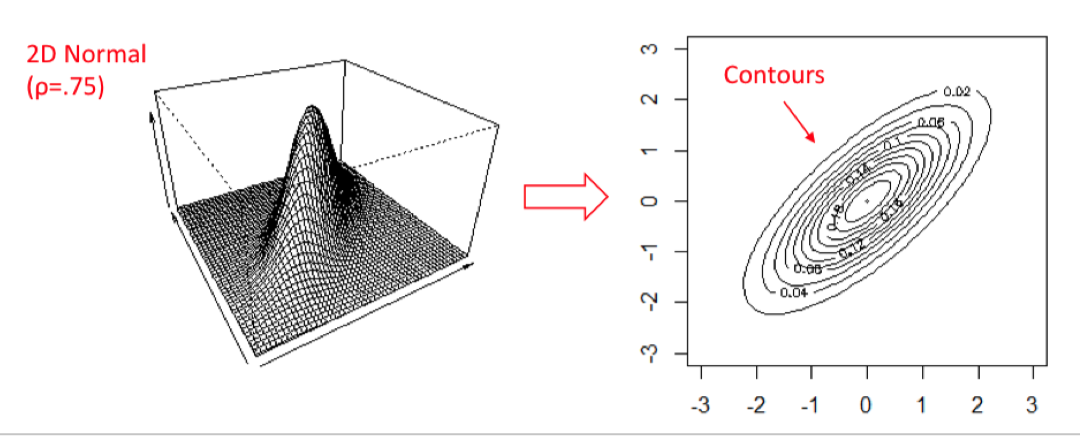
\includegraphics{Notes/Obsidian-Attachments/4-Multivariate-Return-Modelling-8.png}

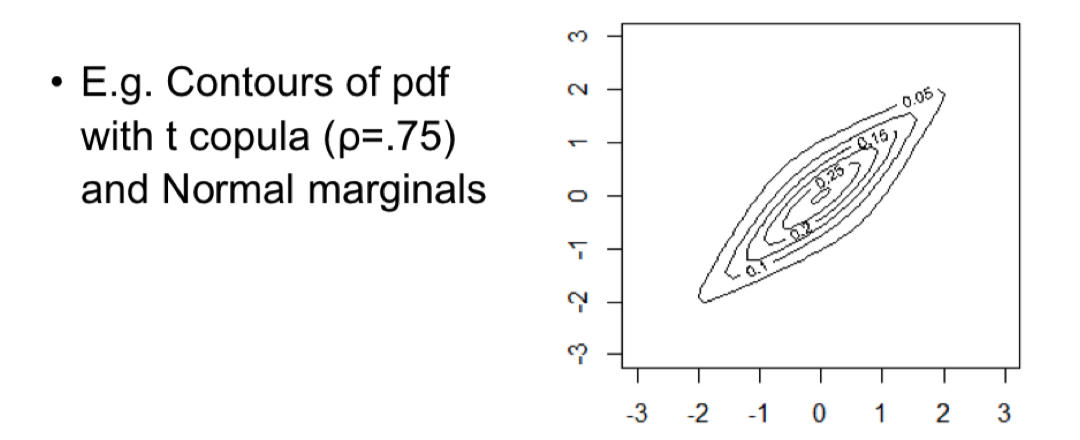
\includegraphics{Notes/Obsidian-Attachments/4-Multivariate-Return-Modelling-9.png}

The ellipses are determined by the covariance matrix of the distributions. This implies a symmetry in the dependency structure, where \textbf{the strength} is the same for positively and negatively correlated variables.

\hypertarget{archimedean-copulas}{%
\section{Archimedean Copulas}\label{archimedean-copulas}}

A Family of copula's whose form is given by
\[
C(u_{1},\dots,u_{d}) = \phi ^{-1}[\phi(u_{1})+\dots+\phi(u_{d})]
\]
Where \(\phi\):

\begin{itemize}
\tightlist
\item
  is a \textbf{continuous convex} generator function
\item
  maps from \([0,1] \to [0,\infty]\)
\item
  \(\phi(0)=\infty, \phi(1)=0\)
\end{itemize}

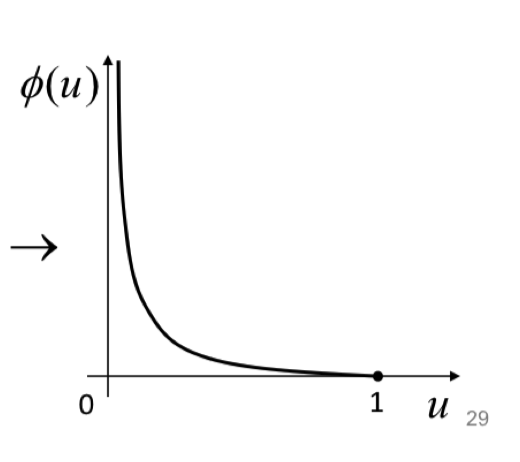
\includegraphics{Notes/Obsidian-Attachments/4-Multivariate-Return-Modelling-10.png}

\begin{quote}
This is just an example of a possible \(\phi\)
\end{quote}

There are infinitely many \(\phi\) but some popular choices for \(\phi\) are:

\begin{longtable}[]{@{}
  >{\raggedright\arraybackslash}p{(\columnwidth - 6\tabcolsep) * \real{0.0598}}
  >{\raggedright\arraybackslash}p{(\columnwidth - 6\tabcolsep) * \real{0.4188}}
  >{\raggedright\arraybackslash}p{(\columnwidth - 6\tabcolsep) * \real{0.4017}}
  >{\raggedright\arraybackslash}p{(\columnwidth - 6\tabcolsep) * \real{0.1197}}@{}}
\toprule\noalign{}
\begin{minipage}[b]{\linewidth}\raggedright
Name
\end{minipage} & \begin{minipage}[b]{\linewidth}\raggedright
Generator \(\phi(t)\)
\end{minipage} & \begin{minipage}[b]{\linewidth}\raggedright
Generator Inverse \(\phi ^{-1}(t)\)
\end{minipage} & \begin{minipage}[b]{\linewidth}\raggedright
Parameter
\end{minipage} \\
\midrule\noalign{}
\endhead
\bottomrule\noalign{}
\endlastfoot
Clayton & \(t^{-\theta}-1\) & \((1+s)^{-1/\theta}\) & \(\theta\geq 0\) \\
Frank & \(-\ln \frac{e^{-\theta t}-1}{\theta^{-\theta}-1}\) & \(-\frac{1}{\alpha}\ln(1+e^{-s}(e^{-\theta}-1))\) & \(\theta\geq 0\) \\
Gumbel & \((-\ln t)^{\theta}\) & \(\exp\{-s ^{-1/\theta}\}\) & \(\theta\geq 1\) \\
\end{longtable}

\begin{quote}
\(\theta\) seems to represent how extreme the function varies between its domain, with larger \(\theta\)'s implying larger values throughout the domain.
\end{quote}

For example, the Clayton generator with \(\theta=0.25\) in blue, and \(\theta=3\) in red.

\begin{Shaded}
\begin{Highlighting}[]
\NormalTok{bottom={-}0.2;top=4;}
\NormalTok{right=1.2;left={-}0.2;}
\NormalTok{{-}{-}{-}}
\NormalTok{y=1/x\^{}\{0.25\}{-}1|0\textless{}=x\textless{}=1|blue}
\NormalTok{y=1/x\^{}\{3\}{-}1|0\textless{}=x\textless{}=1|red}
\end{Highlighting}
\end{Shaded}

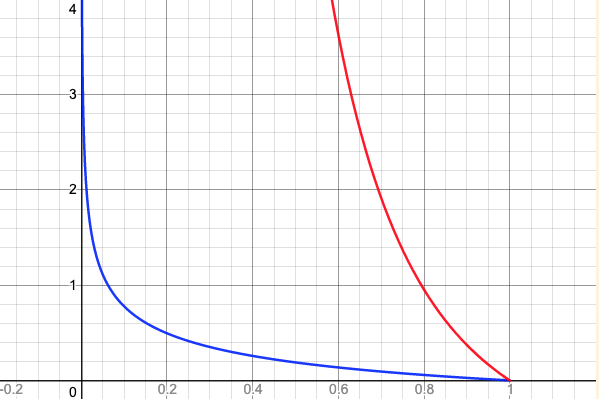
\includegraphics{Notes/Obsidian-Attachments/4-Multivariate-Return-Modelling-12.png}

Samples from the Archimedean copula's:

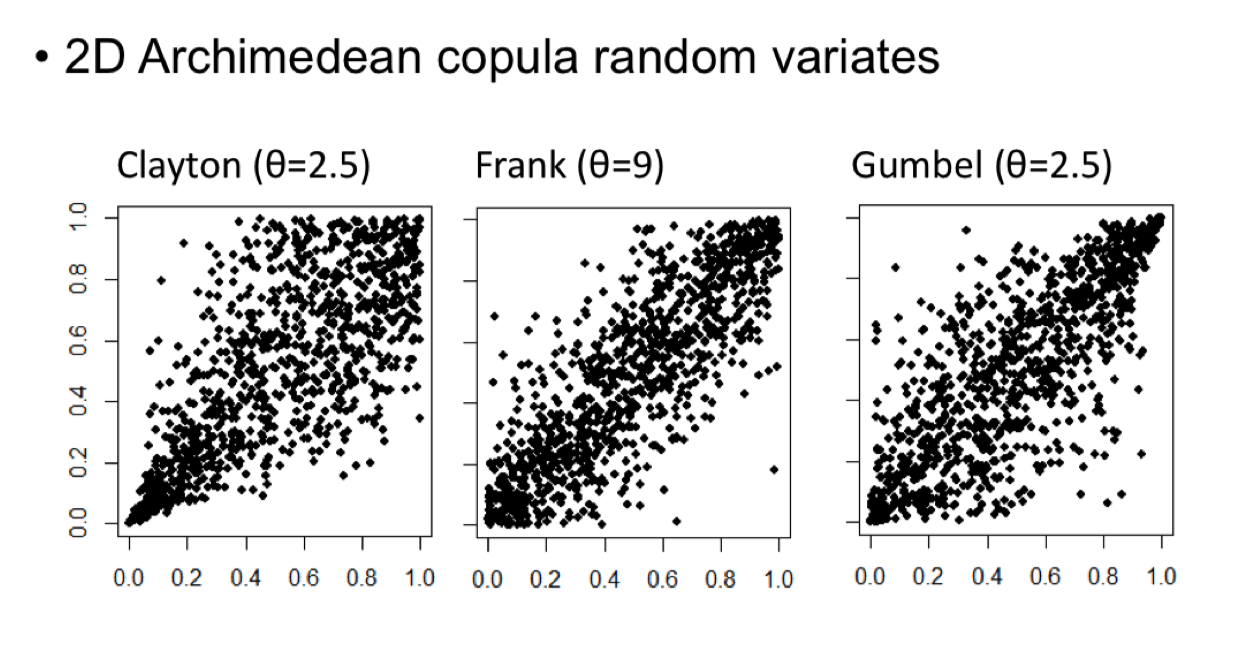
\includegraphics{Notes/Obsidian-Attachments/4-Multivariate-Return-Modelling-11.png}

The dependency contours of each type of archimedean copula's base distribution covariance

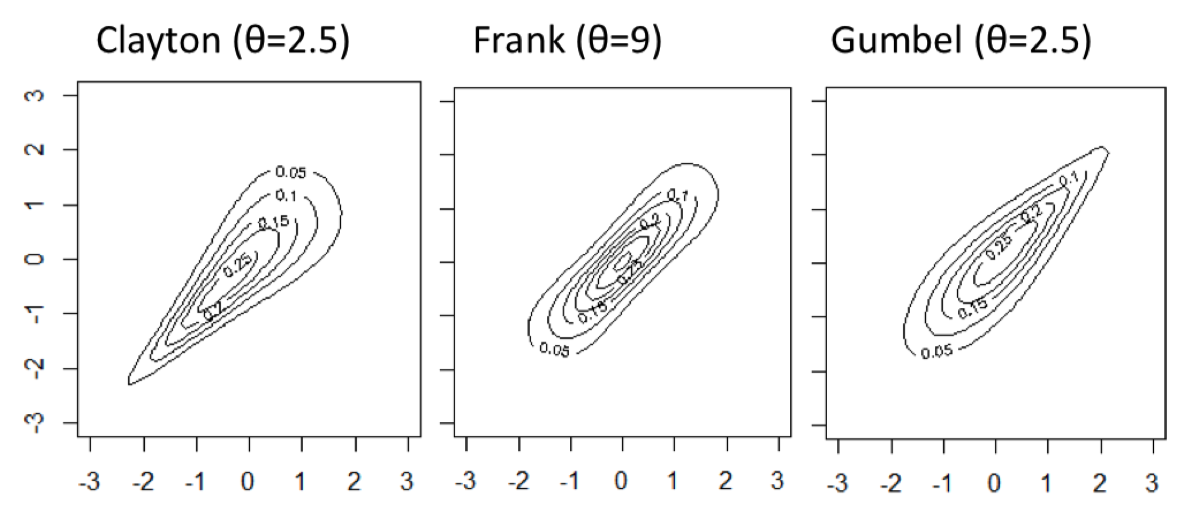
\includegraphics{Notes/Obsidian-Attachments/4-Multivariate-Return-Modelling-13.png}

This plot shows that we can use Archimedean copula's to model \textbf{asymmetric dependencies}, but suffer limitation in \(\geq\) 3 dimensions.

The Archimedean Copula's value is constant for any permutation of coordinates \(u_{1}, \dots, u_{d}\)
\[
\begin{aligned}
C(u_{1}, u_{2}, \dots, u_{d}) &= \phi ^{-1}(\phi(u_{1})+\phi(u_{\mathbf{2}})+\dots+\phi(u_{\mathbf{d}}))\\
&= \phi ^{-1}(\phi(u_{1})+\phi(u_{\mathbf{d}})+\dots+\phi(u_{\mathbf{2}}))\\
\end{aligned}
\]

All pairs of coordinates(variables) have the same dependence, \textbf{which is not the case for elliptical copulas}.

\begin{quote}
There exist copulas that can both model asymmetric dependencies, \textbf{and} differences in pairwise dependence called \textbf{vine copula's}.
\end{quote}

\hypertarget{fitting-copulas}{%
\section{Fitting Copula's}\label{fitting-copulas}}

Given a copula and marginal distributions, the MLE method can be applied to fit multivariate distribution parameters to sample data. This could however lead to a very high number of parameters.

Instead, \emph{pseudo-MLE} could be used to break down the problem into the marginals and copula.
\[
\begin{aligned}
U_{i}^{(j)} = \hat{F}_{j}(X_{i}^{(j)}) \quad \forall \ i, \dots,n \ j = 1, \dots, d
\end{aligned}
\]

\begin{quote}
Each \(n\) uniforms in \(d\) dimensions of the copula can be created from the actual multivariate distribution. Alternatively, the empirical CDF could be used to obtain the uniforms.
\end{quote}

We can then estimate the copula using MLE on the uniforms.

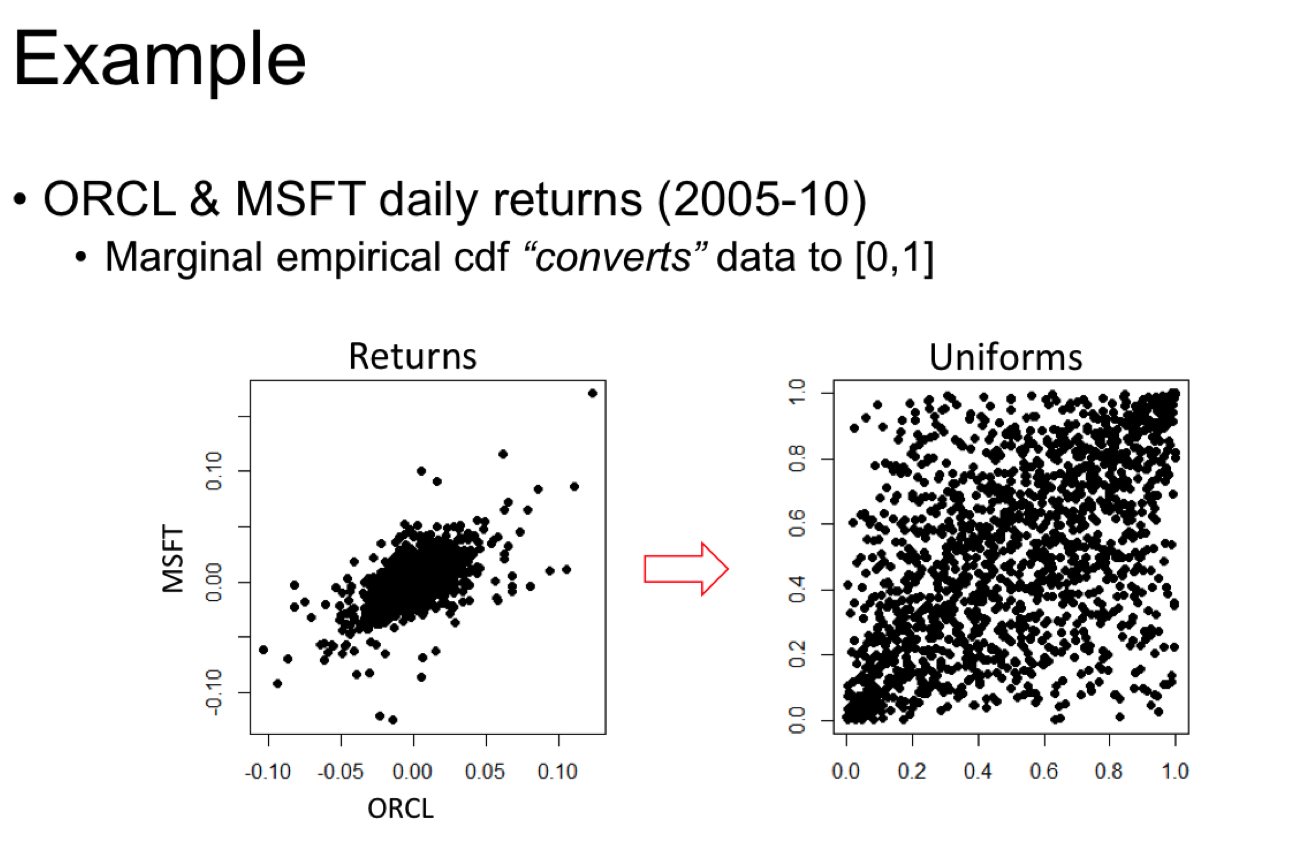
\includegraphics{Notes/Obsidian-Attachments/4-Multivariate-Return-Modelling-14.png}

\begin{quote}
Guess: The uniforms are created by plugging in each asset return into their own marginal CDF.
\end{quote}

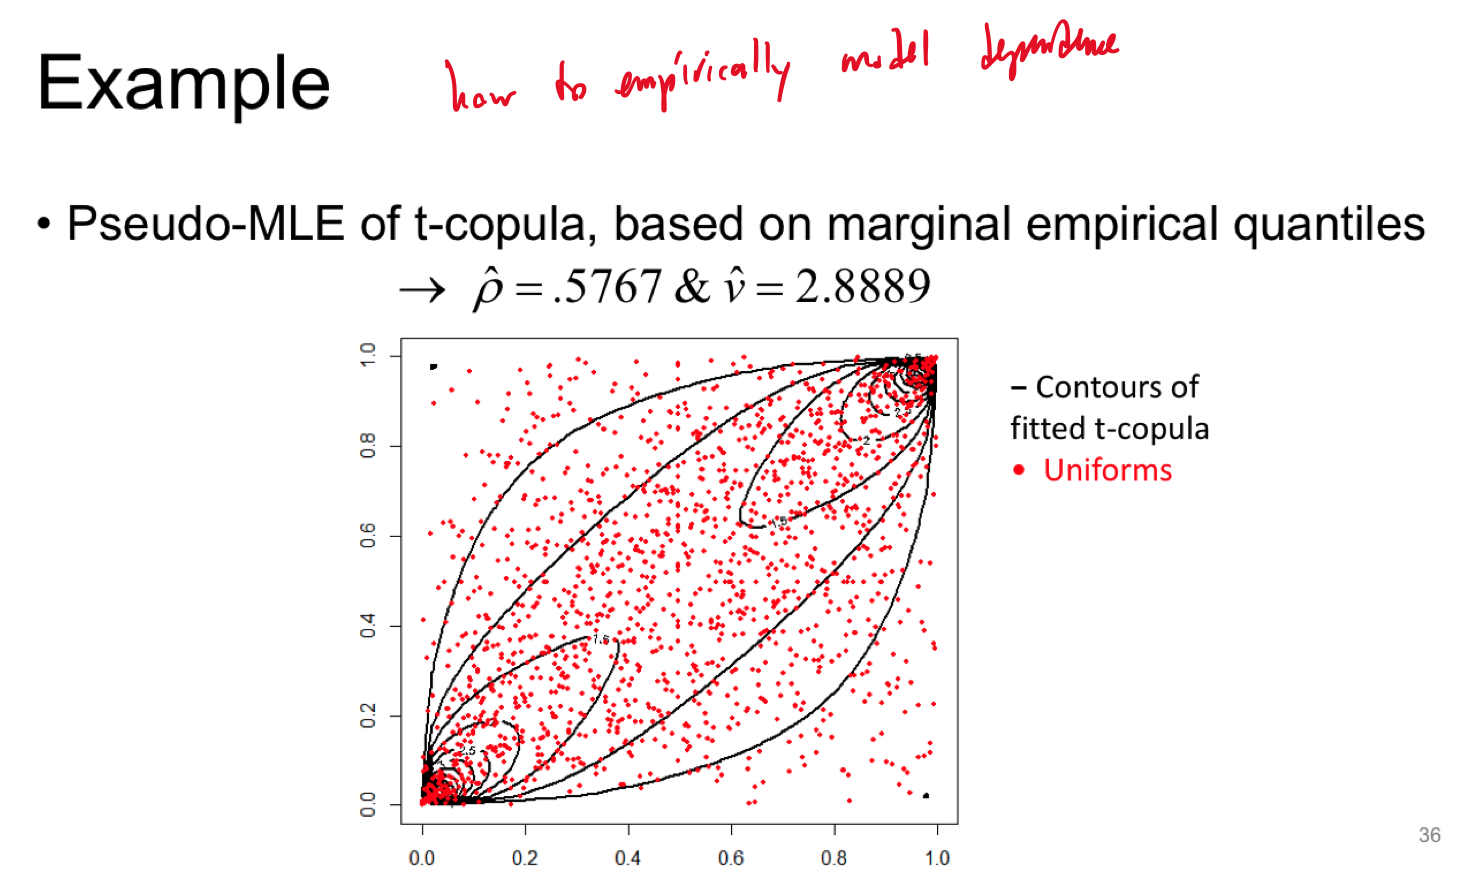
\includegraphics{Notes/Obsidian-Attachments/4-Multivariate-Return-Modelling-15.png}

\begin{quote}
The \emph{pseudo-MLE} can give the uniform marginals used to construct/fit a t-copula.
\end{quote}

\hypertarget{portfolio-theory}{%
\chapter{Portfolio Theory}\label{portfolio-theory}}

Portfolio theory deals with how an asset manager can form a portfolio that optimizes their goals, whether that be lowest risk, highest return, or some other measure of performance.

How to pick stocks is a complicated science and there are many ways to go about it.

\hypertarget{assumptions}{%
\section{Assumptions}\label{assumptions}}

We first make some assumptions when dealing with the theory.
- Static multivariate return distribution determined by assets' mean and covariance.
- This implies a normal or elliptical distribution for returns
- The investors have the same views on mean and variance
- Investors also want minimum risk for maximum return
- Investors measure risk by portfolio's variance
- No borrowing or short-selling restrictions
- No transaction costs

\hypertarget{dealing-with-two-assets}{%
\section{Dealing with Two Assets}\label{dealing-with-two-assets}}

We'll start with a simple example with two risky assets, \(S_{1}, S_{2}\)

We assume that net returns (as time \(0\to t\) ) satisfy:
\[
\left[\begin{array}{c}
R_{1} \\
R_{2}
\end{array}\right] \sim 
N \left( 
\left[ \begin{array}{c}
\mu_{1} \\
\mu_{2}
\end{array} 
\right],
\left[
\begin{array}{cc}
\sigma_{1}^{2}  & \sigma_{12} \\
\sigma_{21}  & \sigma^{2}_{2}
\end{array} \right] 
\right) \quad 
\text{where } R_{i} = \frac{S_{i}(t)-S_{i}(0)}{S_{i}(0)}, i = 1,2
\]

We can form a portfolio with \(x_{i}\) units of asset \(S_{i}\), which gives us the following equation:
\[
\begin{aligned}
V(t=0) &= x_{1}\cdot S_{1}(0)+x_{2}\cdot S_{2}(0)\\
\end{aligned}
\]
We can derive the initial \emph{weights} of each asset that we've invested into using:
\[
w_{i} = \frac{x_{i}S_{i}(0)}{V(0)}
\]

\hypertarget{portfolio-return}{%
\subsection{Portfolio Return}\label{portfolio-return}}

We can calculate the return of this two asset portfolio and show that: \(R_{p} = w_{1}R_{1}+w_{2}R_{2}\)
\[
\begin{aligned}
R_{p} &= \frac{V(t)-V(0)}{V(0)} = \frac{[x_{1}S_{1}(t)+x_{2}S_{2}(t)]-[x_{1}S_{1}(0)+x_{2}S_{2}(0)]}{V(0)}\\
&= \frac{x_{1}[S_{1}(t)-S_{1}(0)]+x_{2}[S_{2}(t)-S_{2}(0)]}{V(0)}\\
&= x_{1} \underset{ \text{Introduce }S_{1}(0) \text{ to get} R_{1}}{ \frac{S_{1}(t)-S_{1}(0)}{S_{1}(0)} \frac{S_{1}(0)}{V(0)} } + x_{2} \underset{  \text{Introduce }S_{2}(0) \text{ to get} R_{2} }{ \frac{S_{2}(t)-S_{2}(0)}{S_{2}(0)} \frac{S_{2}(0)}{V(0)} }\\
&= R_{1} \underbrace{ x_{1}\frac{S_{1}(0)}{V(0)} }_{ w_{1} }+R_{2} x_{2}\underbrace{ \frac{S_{2}(0)}{V(0)} }_{ w_{2} }\\
&= R_{1}w_{1}+R_{2}w_{2}
\end{aligned}
\]
Which shows that the net returns of a portfolio is exactly the weight combination of the net returns of the assets within.

We can also find the distribution of the portfolio returns (which may not surprise you, is just the linear combination of the individual assets returns)

\[
\begin{aligned}
R_{p} &= \underline{w}^{T}\underline{R} = [ w_{1} \ w_{2}] \left[ \begin{array}{c}
R_{1} \\
R_{2}
\end{array} \right]  \quad 
\text{ where } \underline{R} \sim N_{2D}\left( \left[ \begin{array} {l}
\mu_{1} \\
\mu_{2}
\end{array} \right], 
\left[ \begin{array}{cc}
\sigma_{1}^{2} & \sigma_{12} \\
\sigma_{21} & \sigma_{2}^{2}
\end{array}\right]  \right)\\
&\implies R_{p} \sim N_{1D}(\mu_{p},\sigma_{p}) \ \text{ where}\\
\end{aligned}
\]

\[
\begin{aligned}
\mu_{p} &= \mathbb{E}(R_{p}) = \mathbb{\mathbf{E}}[\underline{w}^{T}\underline{R}]\\
&= \underline{w}^{T}\mathbb{E}[\underline{R}] = \underline{w}^{T}\underline{\mu}\\
&= \sum_{i}w_{i}\mu_{i}\\
\\
\sigma_{p}^{2} &= \mathbb{V}[R_{p}] = \mathbb{V}[\underline{w}^{T}\underline{R}]\\
&= \underline{w}^{T} \mathbb{V}(\underline{R})\underline{w} = \underline{w}^{T}\Sigma \underline{w}\\
&= [ w_{1} \ w_{2}] 
\left[ \begin{array}{cc}
\sigma_{1}^{2} & \sigma_{12} \\
\sigma_{21} & \sigma_{2}^{2}
\end{array}\right] \left[ \begin{array}{c}
w_{1} \\
w_{2}
\end{array} \right] \\
&= w_{1}^{2}\sigma_{1}^{2}+2w_{1}w_{2}\sigma_{12}+w_{2}^{2}\sigma_{2}^{2}\\
\\
\therefore R_{p} &\sim N\left( \sum_{i}w_{i}p_{i},  \quad w_{1}^{2}\sigma_{1}^{2}+2w_{1}w_{2}\sigma_{12}+w_{2}^{2}\sigma_{2}^{2}\right)
\end{aligned}
\]

\hypertarget{efficiency-frontier}{%
\section{Efficiency frontier}\label{efficiency-frontier}}

A plot of mean \(\mu\) by standard deviation \(\sigma\) , where you can load up entirely on \texttt{AAPL} with \(w_{1}=1, w_{2}=0\) or entirely on \texttt{PNC} with the opposite.

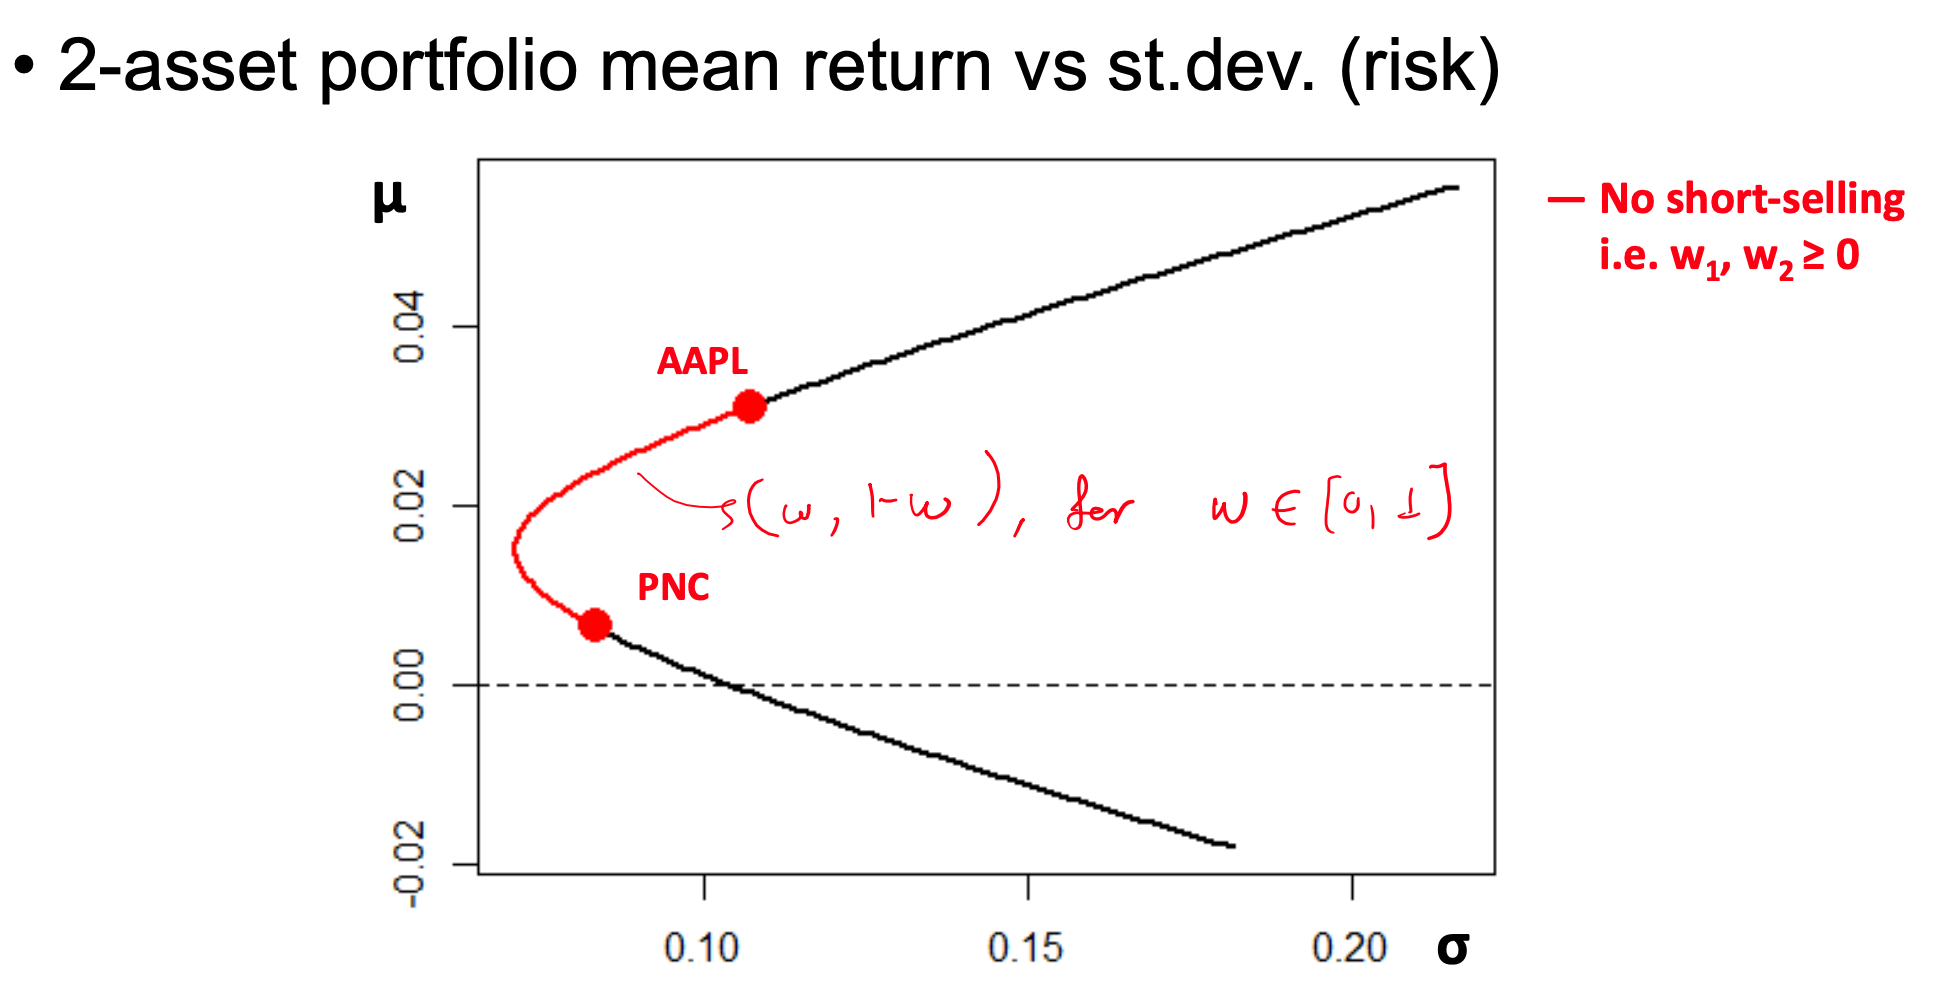
\includegraphics{Notes/Obsidian-Attachments/5-Portfolio-Theory.png}

But how do we know the optimal amount of weight to put in each asset to \textbf{minimize variance}? We can simply find the \(w\) that minimizes the derivative of the variance w.r.t. \(w\)

\[
\begin{aligned}
\text{Let }w_{1} &= w \quad \& \ w_{2}=1-w\\
\implies \sigma_{p}^{2} &= w^{2}\sigma_{1}^{2} + 2w(1-w)\sigma_{12} + (1-w)^{2}\sigma_{2}^{2}\\
\text{Let }\frac{\delta \sigma_{p}^{2}}{\delta w} &= 0\\
0 &= 2w\sigma_{1}^{2}+2(1-w)\sigma_{12}-2w\sigma_{12}-2(1-w)\sigma_{2}^{2}\\
0 &= w(\sigma_{1}^{2}-\sigma_{12}) + (1-w)(\sigma_{12}-\sigma_{2}^{2})\\
0 &= w(\sigma_{1}^{2}+\sigma_{2}^{2}-2\sigma_{12}) + (\sigma_{12}-\sigma_{2}^{2})\\
w &= \frac{-(\sigma_{12}-\sigma_{2}^{2})}{(\sigma_{1}^{2}+\sigma_{2}^{2}-2\sigma_{12})}
\end{aligned}
\]

\hypertarget{multiple-asset-portfolio}{%
\section{Multiple asset portfolio}\label{multiple-asset-portfolio}}

Consider \(n\) risky assets with returns \(R_1, \ldots, R_n\) so that:
\[
\mathbf{R}=\left[\begin{array}{c}
R_1 \\
\vdots \\
R_n
\end{array}\right] \sim N\left(\boldsymbol{\mu}=\left[\begin{array}{c}
\mu_1 \\
\vdots \\
\mu_n
\end{array}\right], \boldsymbol{\Sigma}=\left[\begin{array}{ccc}
\sigma_1^2 & \ldots & \sigma_{1 n} \\
\vdots & \ddots & \vdots \\
\sigma_{n 1} & \cdots & \sigma_n^2
\end{array}\right]\right)
\]
We want to create portfolio using weights \(\mathbf{w}=\left[\begin{array}{lll}w_1 & \cdots & w_n\end{array}\right]^{\top}\) such that: \(\sum_{i=1}^n w_i=\mathbf{w}^{\top} \mathbf{1}=1\)

The distribution of returns for this portfolio would simply be:
\[
\begin{aligned}
\mathbf{R_{p}} &\sim \mathbf{N_{1D}(\mu_{p}, \sigma_{p}^{2})} \ \text{where }\\
&\mathbf{\mu_{p} = \underline{w}^{T}\cdot \underline{\mu}}\\
&\mathbf{\sigma_{p}^{2}=\underline{w}^{T}\cdot\underline{\Sigma}\cdot\underline{w}}
\end{aligned}
\]

When fixing an expected return \(\mu_{p}\), we can derive weights that minimize variance:
\[
min_{w}\{\mathbf{w^{T}\Sigma w}\}\ s.t. \ \mathbf{w^{T}\mu} = \mu_{p}, \mathbf{w^{T}1} = 1
\]

We can use Lagrange multipliers to define the objective function:

\begin{quote}
Lagrange formula: \(\mathcal{L}(x,\lambda) = f(x)+\lambda g(x)\)
If we want to find the max/min of the function \(f(x)\) subject to the constraint \(g(x) = 0\), we can form this Lagrangian and find where it's derivative is 0. In this case, \(x=\underline{w}\) and our constraint \(\mathbf{w^{T}\cdot 1} = 1\) can be represented as \(g(w) = \mathbf{w^{T}\cdot 1} -1\)
\end{quote}

\[
\begin{aligned}
\mathcal{L}(\underline{w},\lambda) &= \underline{w}^{T}\underline{\Sigma}\underline{w} - \lambda(\underline{w}^{T}\cdot \underline{1}-1)\\
\text{Let }\frac{\delta\mathcal{L}}{\delta \underline{w}}&= 0\\
0 &= 2\cdot\underline{\Sigma}\cdot \underline{w}-\lambda\cdot  \underline{1} \\
\implies \underline{w} &= \frac{\lambda}{2}\underline{\Sigma}^{-1}\cdot \underline{1}
\end{aligned}
\]
\[
\begin{aligned}
\text{Given } \underline{w}^{T}\cdot  \underline{1} &= 1 \implies  \underline{1}^{T}\underline{w} = 1\\ \\
\implies& \frac{\lambda}{2}\cdot   \underline{1}^{T}\cdot\underline{\Sigma}^{-1}\cdot  \underline{1} = \underline{1}^{T}\underline{w}  = 1\\
\implies& \lambda = \frac{2}{\underline{1}^{T}\cdot\underline{\Sigma}^{-1}\cdot  \underline{1}}\\
\implies &\underline{w}^{*} = \frac{\frac{2}{\underline{1}^{T}\cdot\underline{\Sigma}^{-1}\cdot  \underline{1}}}{2}\underline{\Sigma}^{-1}\cdot \underline{1}\\
& \quad \ = \frac{\underline{\Sigma}^{-1}\cdot \underline{1}}{\underline{1}^{T}\cdot\underline{\Sigma}^{-1}\cdot  \underline{1}}
\end{aligned}
\]

\begin{quote}
\(\underline{\Sigma}^{-1}\) represents the \href{https://stephens999.github.io/fiveMinuteStats/normal_markov_chain.html}{precision matrix}, where if there is a 0 at \((i,j)\) then \(i\) and \(j\) are conditionally independent (given all other assets are held constant, there is no dependence/correlation between these two assets). If it exists, then it is positive definite.
\end{quote}

\begin{quote}
The numerator is a vector containing the L1 norms of each row's (asset) precision.
The denominator represents the total precision of the entire Precision matrix.
The final value is the scaled weights given to each asset \textbf{depending} on the total precision.
\end{quote}

Instead of only having \(n\) risky assets, we can introduce a risk-free asset with constant return \(R_{f}=\mu_{f}>0\), with variance \(\sigma_{f} =0\). A real life example is a government bond.

With this new asset, we can determine how much to invest in the risky portfolio and the risk-free asset with weights \(w_{p}\) and \((1-w_{p})\).

\begin{itemize}
\tightlist
\item
  Return: \(R=w_{p}R_{p}+(1-w_{p})R_{f}\)
\item
  Mean Return: \(\mathbb{E}[R]=w_{p}\mathbb{E}[R_{p}]+(1-w_{p})\mathbb{E}[R_{f}]=w_{p}\mu_{p}+(1-w_{p})\mu_{f}\)
\item
  Variance of returns: \(\mathbb{V}=\mathbb{V}(w_{p}R_{p}+(1-w_{p}R_{f})) = w_{p}^{2}\mathbb{V}(R_{p})=w_{p}^{2}\cdot \sigma_{p}^{2}\)
\end{itemize}

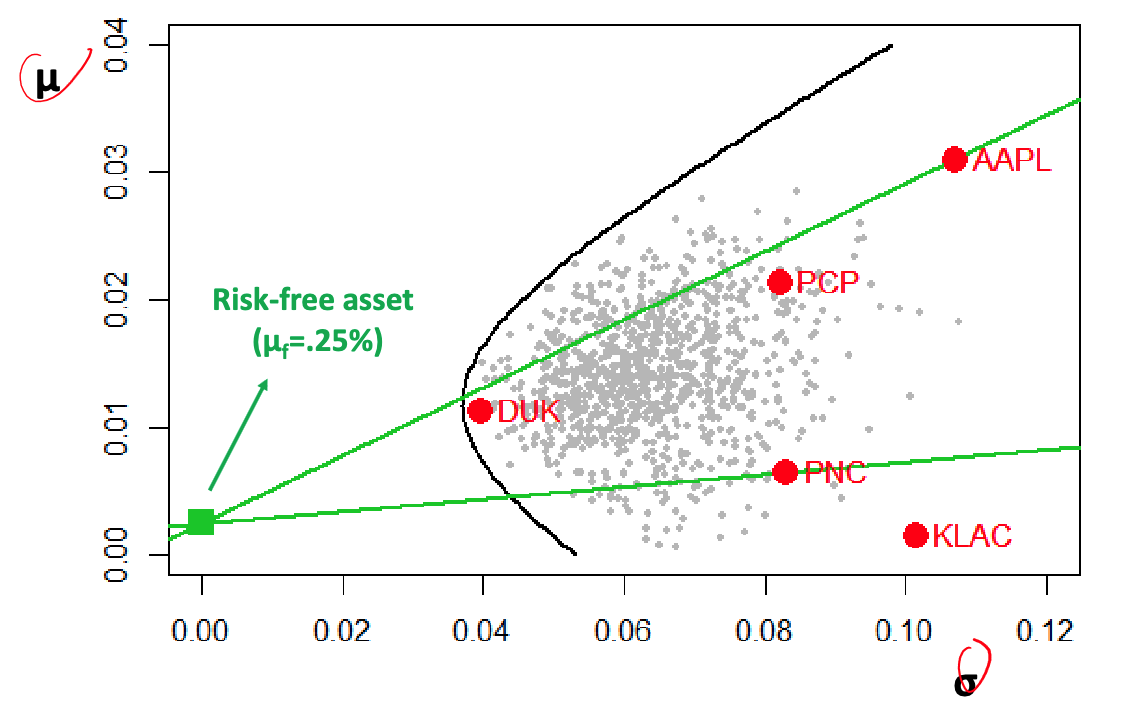
\includegraphics{Notes/Obsidian-Attachments/5-Portfolio-Theory-1.png}

The best portfolio (in terms of risk and return) lie on this green line, where this line is tangent to the efficient frontier.

\begin{quote}
The slope of this line is called the \textbf{Sharpe} ratio, which measure the excess return per unit risk (\textbf{risk premium}).
\end{quote}

The \textbf{tangency portfolio} is exactly the portfolio on the efficient frontier that also belongs to the tangent line. (It is a risky asset only portfolio with \(\mu_{T},\sigma_{T}\))

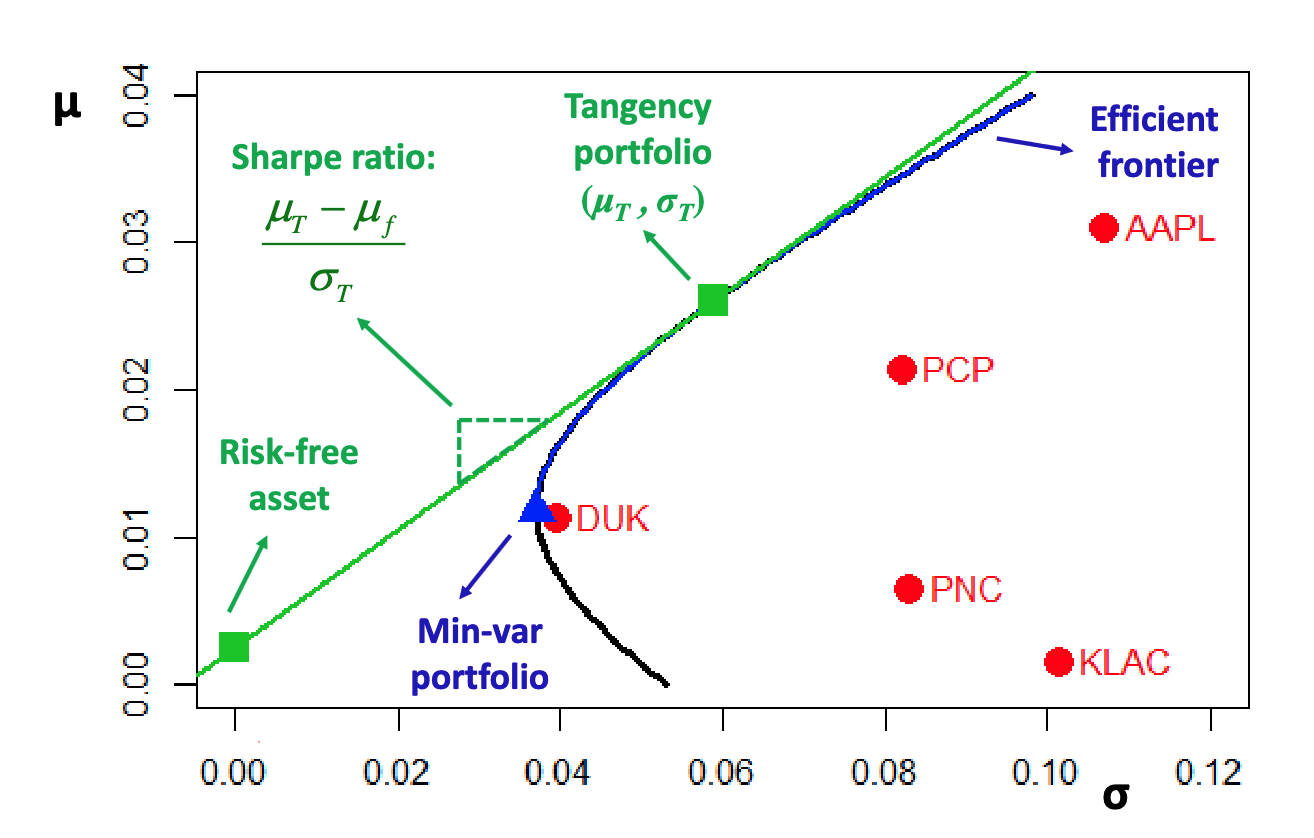
\includegraphics{Notes/Obsidian-Attachments/5-Portfolio-Theory-2.png}

When you have a risk-free asset, the optimal investment strategy is to have a combination of the tangency portfolio and the risk-free asset. To find this tangency portfolio, we \emph{maximize} the Sharpe ratio.

\[
max\left\{ \frac{\mu_{p}-\mu_{f}}{\sigma_{p}} \right\} = max_{w} \left\{ \frac{\mathbf{w^{T}\mu}-\mu_{f}}{\sqrt{ \mathbf{w^{T}\Sigma w} }} \right\} \quad \text{subject to } \mathbf{w^{T}1} = 1
\]

The tangency portfolio weights are given by:
\[
\mathbf{w_{t}} = \frac{\mathbf{\Sigma ^{-1}(\mu}-\mu_{f}\cdot \mathbf{\underline{1}})}{\mathbf{1^{T}\Sigma ^{-1}(\mu}-\mu_{f}\cdot \mathbf{\underline{1}})}
\]

\hypertarget{capm---capital-asset-pricing-model}{%
\section{CAPM - Capital Asset Pricing Model}\label{capm---capital-asset-pricing-model}}

The CAPM theory suggests that all investors hold some form of the tangency/market portfolio. This model assumes the mean-variance analysis \emph{stretched to it's logical consequences} can explain \textbf{all financial market behaviour}.(Widely known to be false)

The slope of the tangency portfolio is also known as the Sharpe Ratio, or \textbf{Market Price of Risk}.

If every investor followed this mean-variance analysis, and the market is in \emph{equilibrium}:
\textgreater idk what it means to be in equilibrium

\begin{itemize}
\tightlist
\item
  Every investor holds some portion of the same tangency portfolio
\item
  The entire financial market will be made up of the \textbf{same} mix of risky assets
\item
  \textbf{Making the tangency portfolio equal to the market value-weighted index}
\end{itemize}

\hypertarget{market-portfolio} } \quad \text{where } \begin{cases}
S_{i} = \text{price of asset i} \\
O_{i} = \text{shares outstanding}
\end{cases}
\]

Therefore the tangency portfolio is exactly a market cap weighted index, such as the S\&P500 or FTSE100.

\hypertarget{capital-market-line}{%
\subsection{Capital Market Line}\label{capital-market-line}}

Every mean-variance efficient portfolio \((\mu_{p},\sigma_{p})\) lies on a straight line, which is determined by
\[
\mu_{p} = \mu_{f} + \frac{\mu_{M}-\mu_{f}}{\sigma_{M}}, \quad \text{where }\begin{cases}
(\mu_{M},\sigma_{M}) = \text{market portfolio} \\
\mu_{f} = \text{risk-free rate}
\end{cases}
\]

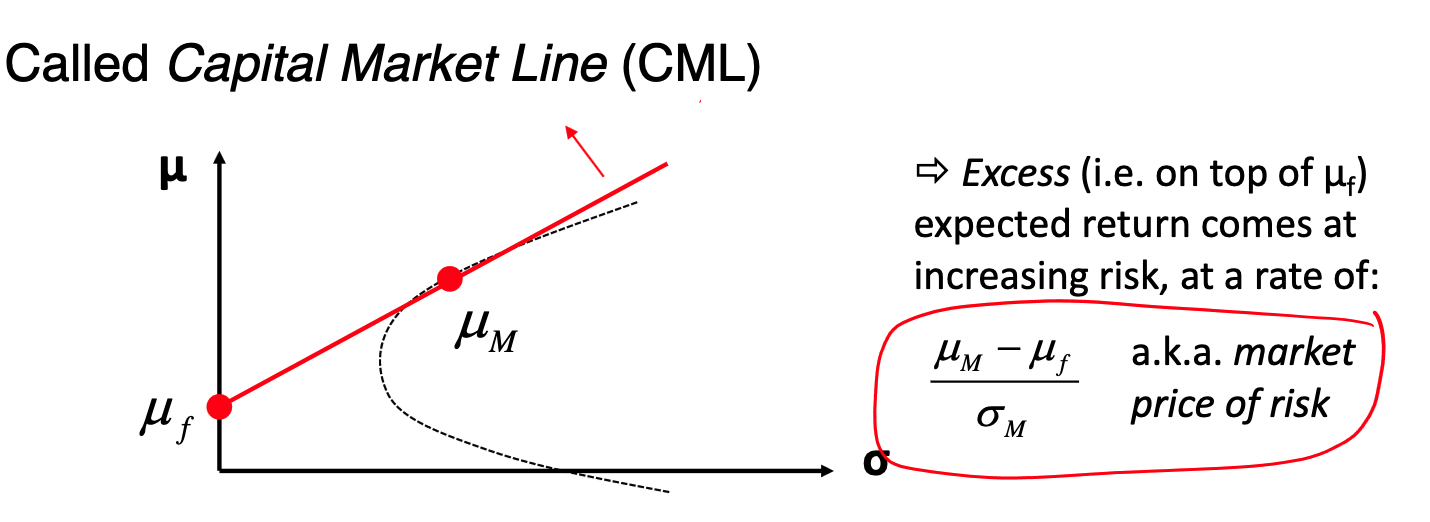
\includegraphics{Notes/Obsidian-Attachments/5-Portfolio-Theory-3.png}

\hypertarget{security-market-line}{%
\subsection{Security Market Line}\label{security-market-line}}

For \textbf{each individual asset}, CAPM implies the following risk/reward relationship (Security Market Line)

\[
\begin{aligned}
\mu_{i} &= \mu_{f} + \beta_{i}\underbrace{ (\mu_{M}-\mu_{f}) }_{ Slope }
\quad \text{Where } \begin{cases}
\beta_{i} = \frac{\sigma_{iM}}{\sigma^{2}_{M}} \\
\sigma_{iM} = Cov(R_{i, R_{M}})
\end{cases}\\
&= \mu_{f} + \left( \frac{\mu_{M}-\mu_{f}}{\sigma_{M}} \right) \cdot \sigma_{p}
\end{aligned}
\]

\begin{itemize}
\tightlist
\item
  \(\beta_{i}\) is different for each asset, it captures how related the return on the given asset is with the Market return.
\item
  \(\sigma_{M}\) is the market risk AKA undiversifiable risk
\item
  Imagine the line is in \((\mu,\beta)\)-space, with slope \((\mu_{M}-\mu_{f})\).
\end{itemize}

To derive this line, we need to find a market portfolio that maximizes the Sharpe ratio (using first order derivative)

\[
\begin{aligned}
f(\underline{w}) &= \frac{\underline{w}^{T}\underline{\mu}-\mu_{f}}{\sqrt{ \underline{w}^{T}\underline{\Sigma}\underline{w} }} = \frac{\underline{w}^{T}\cdot (\underline{\mu}-\underline{1}\mu_{f})}{\sqrt{ \underline{w}^{T}\underline{\Sigma}\underline{w} }} \quad \text{maximized when } \frac{\delta f}{d\underline{w}} = 0\\
\implies 0 &= \frac{(\underline{\mu}-\underline{1}\mu_{f})\cdot\sqrt{ \underline{w}^{T}\underline{\Sigma}\underline{w} } - \frac{1}{2}{(\overbrace{ \underline{w}^{T}\underline{\Sigma}\underline{w}}^{ \sigma_{m}^{2} }})^{-1/2}\cdot 2\underline{\Sigma}\underline{w}\cdot (\overbrace{ \underline{w}^{T}\cdot (\underline{\mu} }^{ \mu_{M} }-\underline{1}\mu_{f})}{\underline{w}^{T}\underline{\Sigma}\underline{w}}\\
&= \frac{(\underline{\mu}-\underline{1}\mu_{f})\sigma_{m}-\frac{1}{\sigma_{M}}\underline{\Sigma}\underline{w}(\mu_{M}-\mu_{f})}{\sigma_{M}^{2}}\\
\implies (\underline{\mu}-\underline{1}\mu_{f}) &= \frac{1}{\sigma_{M}^{2}\underline{\Sigma}\underline{w}(\mu_{M}-\mu_{f})}\\
\implies \left[ \begin{array}{c}
\mu_{1}-\mu_{f} \\
\vdots \\
\mu_{n}-\mu_{f}
\end{array}  \right] 
&= \frac{\mu_{M}-\mu_{f}}{\sigma_{M}^{2}}\cdot 
\left[ \begin{array}{c}
Cov(R_{1},R_{M}) \\
\vdots \\
Cov(R_{n},R_{M})
\end{array} \right] \\
&= \frac{(\mu_{M}-\mu_{f})}{\sigma_{M}^{2}}\cdot \left[ \begin{array}{c}
\sigma_{1,M} \\
\vdots \\
\sigma_{n,M}
\end{array} \right] 
\end{aligned}
\]

This is because \(Cov(\underline{R}, R_{M}) = Cov(\underline{R},\underline{w}^{T}\cdot \underline{R}) = \underline{w}^{T}\underbrace{ Cov(\underline{R},\underline{R}) }_{ \underline{\Sigma} } = \underline{w}^{T}\underline{\Sigma}\)

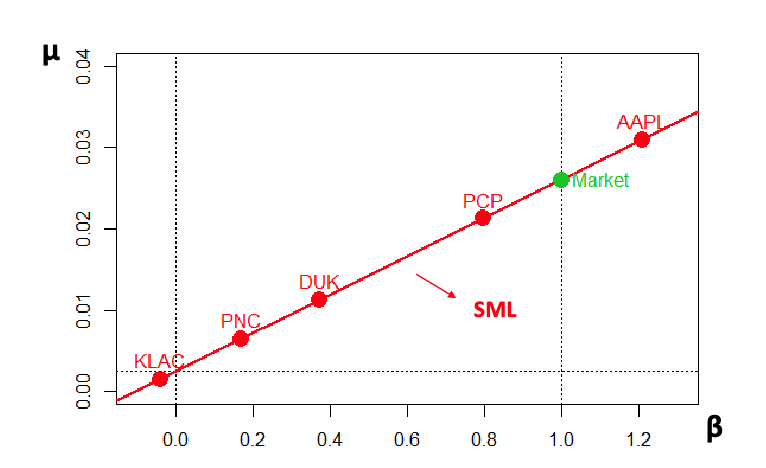
\includegraphics{Notes/Obsidian-Attachments/5-Portfolio-Theory-4.png}

\hypertarget{ex-find-market-portfolio-weights-and-sml-with-n-i.i.d-assets}{%
\subsubsection{\texorpdfstring{Ex: Find market portfolio weights and SML with \(N\) i.i.d assets}{Ex: Find market portfolio weights and SML with N i.i.d assets}}\label{ex-find-market-portfolio-weights-and-sml-with-n-i.i.d-assets}}

Each asset \(\sim N(\mu,\sigma^{2})\) returns and the risk-free return \(\mu_{f}<\mu\).
\[
\left[ \begin{array}{c}
R_{1} \\
\vdots \\
R_{N}
\end{array} \right] \sim N_{N \ Dim}(\underline{\mu} = \mu \cdot  \underline{1}, \underline{\Sigma} = \sigma^{2}\cdot \underline{I})
\]
So we know:
\[
\forall \ \underline{w} \quad s.t. \ \underline{w}^{T}\cdot  \underline{1} = 1 \implies \underline{w}^{T}\cdot\mu\cdot 1 = \mu
\]
Which implies that the market portfolio is equal to the minimum variance portfolio.

\[
\begin{aligned}
\underline{w}^{\star} &= \frac{\underline{\Sigma}^{-1}\cdot  \underline{1}}{\underline{1}^{T}\underline{\Sigma}^{-1}\cdot   \underline{1}} = \frac{\frac{1}{\sigma^{2}}\underline{I}\cdot \underline{1}}{\frac{1}{\sigma^{2}} \underline{1}^{T}\underline{I}\cdot  \underline{1}} = \frac{\underline{1}}{N}\\
\implies \underline{w} &= \frac{\underline{1}}{N} = \left[ \begin{array}{c}
\frac{1}{N} \\
\vdots \\
\frac{1}{N}
\end{array} \right] \implies w_{i} = \frac{1}{N} \ \forall i = 1,\dots,N\\
\implies \text{min variance } &= \underline{w}^{T}\underline{\Sigma}\underline{w}\\
&= \left( \frac{1}{N} \right)^{2}\cdot  \underline{1}^{T}(\sigma^{2}\cdot \underline{I})\cdot  \underline{1}\\
&= \frac{\sigma^{2}}{N}
\end{aligned}
\]

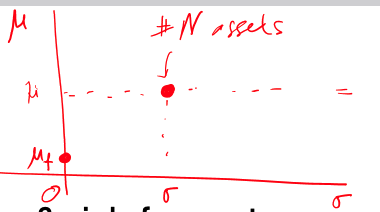
\includegraphics{Notes/Obsidian-Attachments/5-Portfolio-Theory-5.png}

\hypertarget{security-characteristic-line}{%
\subsection{Security Characteristic Line}\label{security-characteristic-line}}

The \(\beta_{i}\)'s are found empirically, by regressing (\(R_{i}-R_{f}\)) on (\(R_{M}-R_{f}\))
- Where \(R_{M}\) is the market return (Proxy by large market index, ex S\&P500)
- \(R_{f}\) is the risk free rate (proxy by T-bill)

\[
(R_{i,t} - R_{f,t}) = \beta_{i}(R_{M,t}-R_{f,t})+\epsilon_{t}, \quad \text{ where } \epsilon_{t} \sim N(0,\sigma^{2}_{\epsilon,i})
\]

By fitting this, we can then extract the \(\beta_{i}\)'s!

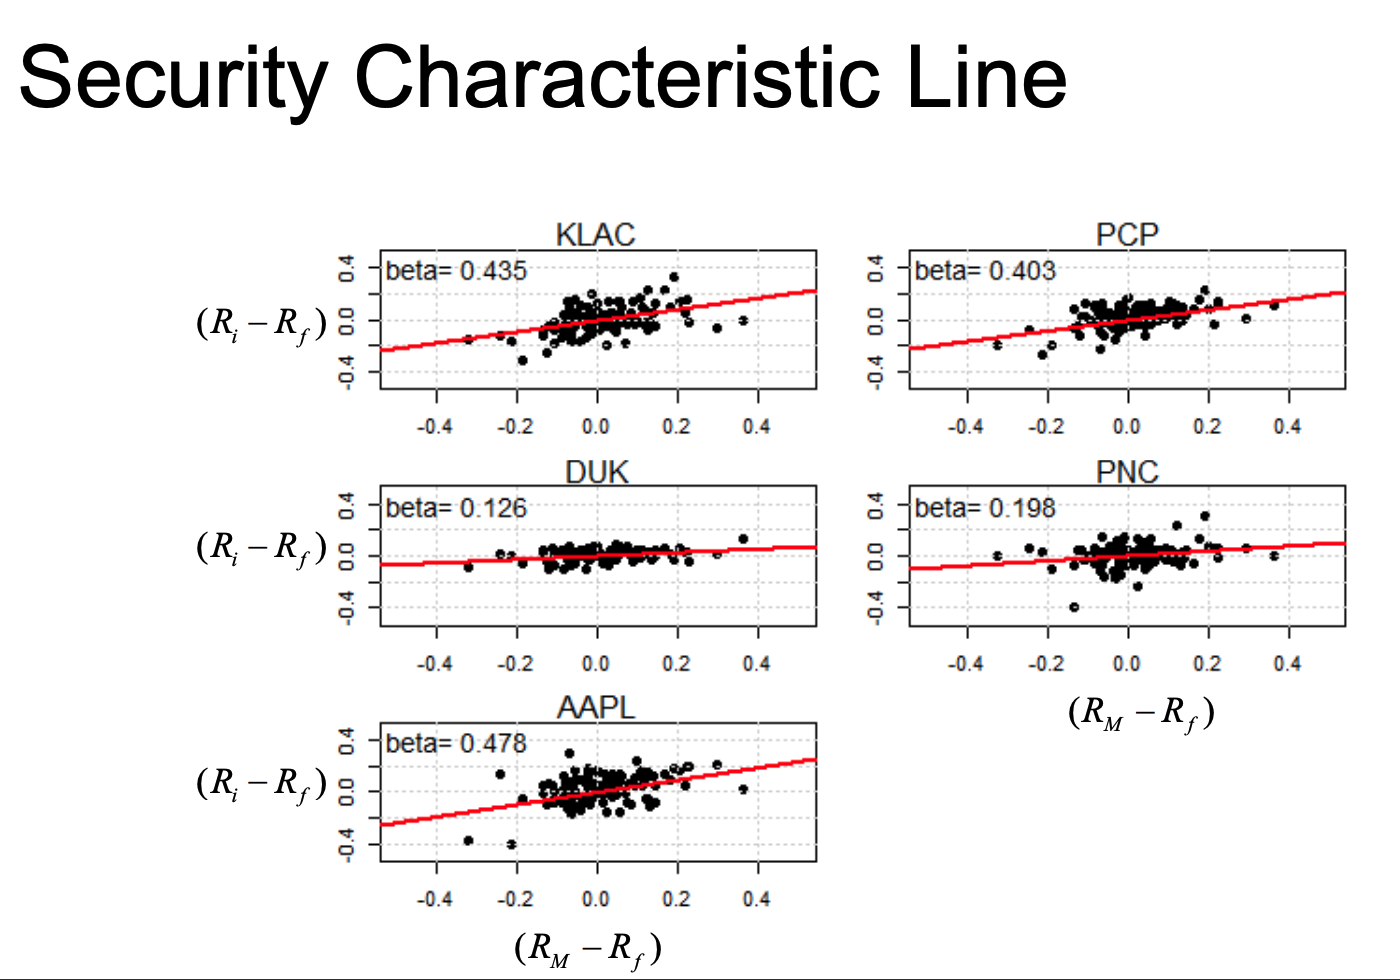
\includegraphics{Notes/Obsidian-Attachments/4-Factor-Models.png}

However the mean expected return is much different than the actual return. Therefore the CAPM model doesn't work very well, or hold.

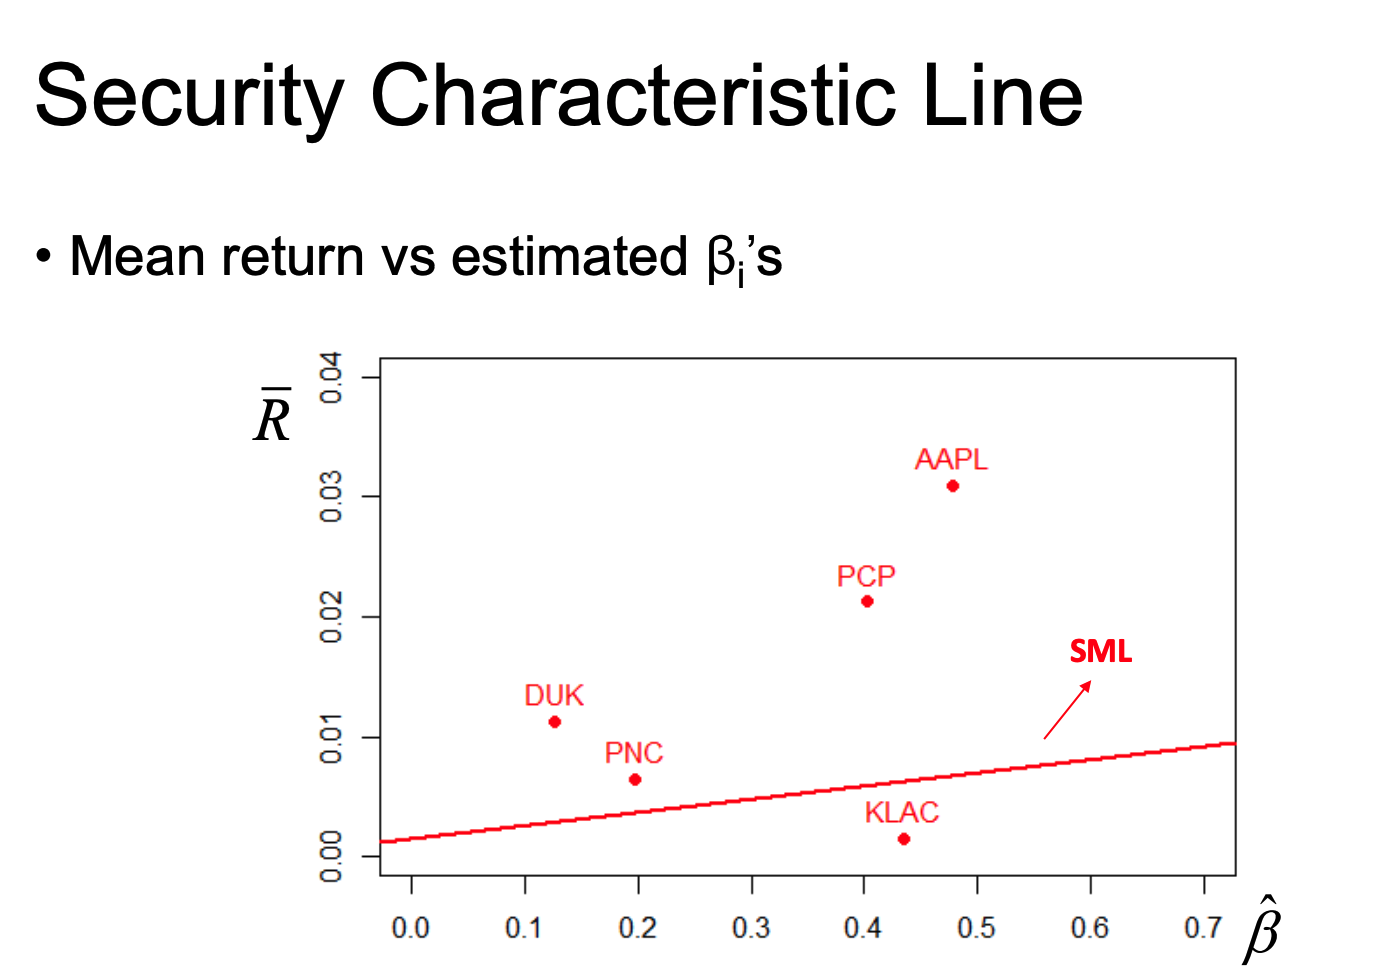
\includegraphics{Notes/Obsidian-Attachments/4-Factor-Models-1.png}

An iteration of this model includes an intercept, \(\alpha\)
\[
(R_{i,t} - R_{f,t}) = \alpha_{i} + \beta_{i}(R_{M,t}-R_{f,t})+\epsilon_{t}
\]
Finding the mean and variance:
\[
\begin{aligned}
\mu_{i} = \mathbb{E}[R_{i}] &= \mathbb{E}[R_{f,t}+\alpha_{i}+\beta_{i}(R_{M,t}-R_{f,t})+\epsilon_{t}]\\
&= \underbrace{ \mathbb{E}[R_{f}] }_{ R_{f} } + \alpha_{i} + \beta_{i}\underbrace{ \mathbb{E}[R_{m}-R_{f}] }_{ \mu_{m - R_{f}} } + \underbrace{ \mathbb{E}[\epsilon_{t}] }_{ =0 }\\
&= R_{f} + \alpha_{i} + \beta_{i}(\mu_{m}-R_{f})\\
\\
\sigma^{2}_{i} = \mathbb{V}[R_{i}] &= \mathbb{V}[\underbrace{ R_{f}+\alpha_{i} }_{ Var = 0 }+\beta_{i}(R_{m}-R_{f})+\epsilon_{i})]\\
&= \mathbb{V}[\beta_{i}(R_{m}-\underbrace{ R_{f} }_{ Var = 0 }] + \mathbb{V}[\epsilon_{i}]\\
&= \beta_{i}^{2} \cdot \mathbb{V}[R_{M}] + \sigma^{2}_{\epsilon, i}\\
&= \beta^{2}_{i}\cdot \sigma^{2}_{m}+\sigma^{2}_{\epsilon,i}
\end{aligned}
\]

Time doesn't matter for the risk free or market returns

\hypertarget{alpha-beta}{%
\subsubsection{Alpha \& Beta}\label{alpha-beta}}

An asset's beta \(\beta_{i}\) can be seen as a measure of both risk \& reward
\[
CAPM \to \mu_{f}  = \mu_{f} + \beta_{i}(\mu_{M}-\mu_{f}) \implies \mu_{i} = \mu_{f} + \beta_{i}\underbrace{ \left(\frac{\mu_{M}-\mu_{f}}{\sigma_{M}}  \right)}_{ \text{Sharpe Ratio} }\sigma_{M}
\]

\(\beta_{i}\) measures extent of the return of a given asset is related to the market

\begin{quote}
\emph{If you believe in CAPM, then the bigger beta is, the more risk you will have but also the more reward you will have.}
\end{quote}

\(\alpha_{i}\) measure how much the asset outperforms the market consistently, the amount returned on top of the \(\beta_{i}\)

\hypertarget{legacy-of-capm}{%
\subsection{Legacy of CAPM}\label{legacy-of-capm}}

CAPM is wrong. A lot of it's assumptions do not hold in reality.

However, it had immense practical impact on investing, specifically in terms of
- Diversification: concept of decreasing risk by spreading portfolio over different assets
- Index investing: justification for common investing strategy of tracking some broad index with mutual funds or ETF's
- Benchmarking: Measuring performance of investment relative to market / index

\hypertarget{performance-evaluation}{%
\subsection{Performance Evaluation}\label{performance-evaluation}}

CAPM says the best portfolio you can create is the tangency/market portfolio. This implies the best you can do is get the broadest index and combine it with a T-bill.

\begin{quote}
Aside: In the past, you needed to use a mutual fund because exchange traded funds didn't exist. Thats how most people invested, even though they cost high fees as there was a lot of human involvement.
\end{quote}

There are several ways to measure an asset's performance, based on CAPM

Sharpe ratio: (excess return per unit risk)
\[
S_i=\frac{\mu_i-\mu_f}{\sigma_i}
\]

\begin{itemize}
\tightlist
\item
  If you combine different assets, you can reduce the \(\sigma_{i}\) of the portfolio, so it's not objective because two assets may be really risky, but negatively correlated reducing \(\sigma_{i}\).
\item
  It doesn't however measure how correlated a portfolio is to the market.
\end{itemize}

Treynor index: (excess return per unit non-diversifiable risk)
\[
\quad T_i=\frac{\mu_i-\mu_f}{\beta_i}
\]

\begin{itemize}
\tightlist
\item
  You would look at this to find the best return
\end{itemize}

Jensen's alpha: (excess return on top of the return explained by the market)
\[
\quad \alpha_i=\hat{\alpha}_i
\]

\begin{itemize}
\tightlist
\item
  Usually the most important measure a portfolio manager tries to use to convince people to invest in them.
\end{itemize}

\hypertarget{factor-models}{%
\chapter{Factor Models}\label{factor-models}}

\hypertarget{three-factor-models}{%
\section{Three Factor models}\label{three-factor-models}}

The CAPM model assumes the market is a single factor that drives asset returns.
- In practice, CAPM does not adequately describe real-world returns

We can improve this model by including more factors in the regression.

There are three types of factor models we will look at:

\begin{itemize}
\tightlist
\item
  Macroeconomic: Factors are \emph{observable} economic and financial time series data (eg return of the S\&P 500)
\item
  Fundamental: Created explicitly or implicitly from observable asset characteristics
\item
  Statistical (Latent variable model): Factors are unobservable and extracted from asset returns
\end{itemize}

All three types follow some form of
\[
\begin{aligned}
R_{i}(t) = \beta_{i,0} + \beta_{i,1}F_{1}(t)+\dots+\beta_{i,p}F_{p}(t)+\epsilon_{i}(t), \quad \forall \begin{cases}
i=1,\dots, N \\
t \in \mathbb{R}
\end{cases}
\end{aligned}
\]
where:

\begin{itemize}
\tightlist
\item
  \(R_{i}(t)\) is return on the \(i^{th}\) asset at time t
\item
  \(F_{j}(t)\) is the \(j^{th}\) common factor at time t
\item
  \(\beta_{i,j}\) is the factor loading/beta of \(i^{th}\) asset on the \(j^{th}\) factor
\item
  \(\epsilon_{i}(t)\) is the idiosyncratic/unique return of asset \(i^{th}\)
\end{itemize}

We want the errors to be independent from the factors,
\[
Cov[\epsilon(t), F(t)] = 0
\]

In matrix form,

\[
\begin{aligned}
& \Leftrightarrow \\
& {\left[\begin{array}{c}
R_1(t) \\
\vdots \\
R_N(t)
\end{array}\right] }=\left[\begin{array}{c}
\beta_{1,0} \\
\vdots \\
\beta_{N, 0}
\end{array}\right]+\left[\begin{array}{ccc}
\beta_{1,1} & \cdots & \beta_{1, p} \\
\vdots & \ddots & \vdots \\
\beta_{N, 1} & \cdots & \beta_{N, p}
\end{array}\right]\left[\begin{array}{c}
F_1(t) \\
\vdots \\
F_p(t)
\end{array}\right]+\left[\begin{array}{c}
\varepsilon_1(t) \\
\vdots \\
\varepsilon_p(t)
\end{array}\right] \\
& \Leftrightarrow \\
& \mathbf{R}(t)=\boldsymbol{\beta}_0+\boldsymbol{\beta}^{\top} \mathbf{F}(t)+\boldsymbol{\varepsilon}(t)
\end{aligned}
\]

The factors \(F_{j}(t)\) are stationary with moments:
\[
\begin{aligned}
R(t) &= \beta_{0} + \beta^{T}F(t) + \epsilon(t)\\
\\
\mu_{r} &= \mathbb{E}(R(t)) = \mathbb{E}[\beta_{0} + \beta^{T}F(t) + \epsilon(t)]\\
&= \beta_{0}+\beta^{T}\underbrace{ \mathbb{E}[F(t)] }_{ \mu_{F} } + \underbrace{ \mathbb{E}[\epsilon(t)] }_{ 0 }\\
&= \beta_{0} + \beta^{T}\mu_{F}\\
\\
\Sigma_{R} &= \mathbb{V}[\beta_{0}+\beta^{T}F(t) +\epsilon(t)]\\
&\underbrace{= \mathbb{V}[\beta^{T}F(t)] + \mathbb{V}[\epsilon(t)]}_{ \text{As } F(t)\text{ indep of } \epsilon_(t)}\\
&= \beta^{T}\underbrace{ \mathbb{V}[F(t)] }_{ \Sigma_{F} }\beta+\Sigma_{\epsilon}\\
&= \beta^{T}\Sigma_{F}\beta+\underbrace{ \Sigma_{\epsilon} }_{ \text{Diagonal} }
\end{aligned}
\]

We can also find the moments of the portfolio with weights \(w = [w_{1}, \dots w_{N}]^{T}\)
\[
\begin{aligned}
R_{port} = w^{T}R \implies \begin{cases}
\mu_{port} = \mathbb{E}[R_{port}] = w^{T}\mathbb{E}[R] = w^{T}(\beta_{0}+\beta_{\mu_{F}}) \\
\sigma^{2}_{port} = \mathbb{V}[R_{port} = \mathbb{V}[w^{T}R] = w^{T}\mathbb{V}[R]w = w^{T}(\beta^{T}\Sigma_{F}\beta+\Sigma_{\epsilon})w
\end{cases}
\end{aligned}
\]

\hypertarget{factor-model-assumptions}{%
\section{Factor Model Assumptions}\label{factor-model-assumptions}}

\begin{itemize}
\tightlist
\item
  Factors \(F_j(t)\) are stationary, with moments:
  \[
  E[\mathbf{F}(t)]=\boldsymbol{\mu}_F \quad \& \quad \operatorname{Var}[\mathbf{F}(t)]=\boldsymbol{\Sigma}_F
  \]
\item
  Asset-specific errors \(\varepsilon_i(t)\) are uncorrelated with common factors:
  \[
  \operatorname{Cov}[\mathbf{\varepsilon}(t), \mathbf{F}(t)]=\mathbf{0}
  \]
\item
  Errors are serially \& contemporaneously uncorrelated across assets
  \[
  \operatorname{Var}[\boldsymbol{\varepsilon}(t)]=\operatorname{diag}\left[\left\{\sigma_{\varepsilon_i}^2\right\}_{i=1, \ldots, N}\right]=\boldsymbol{\Sigma}_{\varepsilon} \quad \& \operatorname{Cov}[\boldsymbol{\varepsilon}(t), \boldsymbol{\varepsilon}(s)]=\mathbf{0}
  \]
\end{itemize}

\hypertarget{time-series-regression-models}{%
\section{Time Series Regression Models}\label{time-series-regression-models}}

Consider model for which factor values are known (e.g.~macro/fundamental model)

Estimate betas \& risks (variances) one asset at a time, using time series regression

\begin{itemize}
\tightlist
\item
  For each fixed \(i=1,\dots N\), fit regression model:
  \[
  R_{i}(t) = = \beta_{i,0} + \beta_{i,1}F_{1}(t)+ \dots + \beta_{i,p}F_{p}(t) + \epsilon_{i}(t)
  \]
\end{itemize}

Most models will always include some proxy for the overall economy (eg the market)

Instead of Fama-French, there is BARRA which uses the cross section of returns? Still regression tho

\hypertarget{fama-french-3-factor-model}{%
\subsection{Fama-French 3 Factor Model}\label{fama-french-3-factor-model}}

Additionally to the market, they looked at two other factors that are consistent over many datasets and time periods.

\textbf{Small Minus Big: (SMB)}
One factor tries to capture the size(market cap) of the company/stock, which empirically showed that size played a role in its return

\begin{itemize}
\tightlist
\item
  Regressed returns on how companies of a certain size/group did

  \begin{itemize}
  \tightlist
  \item
    They took the smallest and biggest companies, and looked at their avg return over some period, creating a difference to use to separate the groups of companies
  \end{itemize}
\end{itemize}

\textbf{High Minus Low (HML):}
The second factor looks at whether a company is a \textbf{value} one or not. Measured using book-to-market ratio.

\begin{quote}
These two factors were found to have statistically significant coefficients in multiple regression.
\end{quote}

People frequently use the factor model to estimate the return covariance matrix.
They can use the sample covariance matrix of the factors and apply the beta vector in order to obtain the return covariance matrix

\[
\operatorname{Var}(\mathbf{R})=\hat{\boldsymbol{\Sigma}}_R=\hat{\boldsymbol{\beta}}^{\top} \hat{\boldsymbol{\Sigma}}_F \hat{\boldsymbol{\beta}}+\hat{\boldsymbol{\Sigma}}_{\varepsilon}
\]
where:
\[
\begin{aligned}
& \hat{\boldsymbol{\beta}}=\text { beta coefficient matrix (from regressions) } \\
& \hat{\boldsymbol{\Sigma}}_F=\text { factor sample covariance matrix } \\
& \hat{\boldsymbol{\Sigma}}_{\varepsilon}=\text { diagonal error variance matrix (from residuals) }
\end{aligned}
\]
This gives more stable estimates than sample covariance.

\hypertarget{statistical-factor-models}{%
\section{Statistical Factor Models}\label{statistical-factor-models}}

In this model, the factors are \textbf{unknown (latent) and unobserved}. This implies that we need to estimate both \(\beta\) and \(F\).

Unusual constraint: Because the factors are uncorrelated (not necessarily i.i.d.)
\[
\Sigma_{F} = Cov(F)= I \sigma_F \quad \& \quad \mu_{F}=\mathbb{E}(F) = 0
\]

This gives us the resulting moments of the returns:
\[
\begin{aligned}
\mu_{R} &= \mathbb{E}[R] = \mathbb{E}[\beta_{0}+\beta^TF + \epsilon] = \beta_{0}+\beta^{T}\underbrace{ \mathbb{E}[F] }_{ 0 }+\underbrace{ \mathbb{E}[\epsilon] }_{ 0 } = \beta_{0}\\
\\
\Sigma_{R} &= \mathbb{V}[R] = \mathbb{V}[\boldsymbol{\beta}_{0}+\boldsymbol{\beta}^{T}F+\boldsymbol{\epsilon}] = \boldsymbol{\beta}^{T}\mathbb{V}[F]\boldsymbol{\beta}+\boldsymbol{\Sigma_{\epsilon} = \beta^{T}(I\cdot \sigma_{F})\beta+\Sigma_{\epsilon}}
\end{aligned}
\]

\hypertarget{principle-component-analysis-pca}{%
\section{Principle Component Analysis (PCA)}\label{principle-component-analysis-pca}}

This technique helps reduce the dimensionality of a problem. Consider a factor model without errors:
\[
\mathbf{R}(t) = \boldsymbol{\beta}_{0}+\boldsymbol{\beta}^{T}\mathbf{F}(t) \implies \boldsymbol{\Sigma_{R}=\beta^{T}\Sigma_{F}\beta}
\]

Given a set of N assets, we can construct a set of variables (components) capturing most of the variability.

\begin{itemize}
\tightlist
\item
  PCA is a linear transformation
\item
  The goal is to capture as much variation as possible.
\end{itemize}

When we apply PCA to the statistical model, we find \(n\) factors set as the PCA components. These components are \textbf{uncorrelated}, and have \textbf{maximum variance.}

\[
F_{1},\dots,F_{n} \text{ are factors which are the Principle Components}
\]
\[
\begin{aligned}
F_{1} &= \gamma_{1}^{T}\mathbf{R} = \gamma_{11}R_{1}+\dots+\gamma_{1n}R_{n}\\
\vdots\\
F_{n} &= \gamma_{n}^{T}\mathbf{R} = \gamma_{n1}R_{1}+\dots+\gamma_{nn}R_{n}\\
\end{aligned}
\]

Where each factor:

\[
\begin{aligned}
F_{i} &= \gamma_{i}^{T}\mathbf{X} \quad \text{Maximizes } \ Var(F_{i})=\boldsymbol{\gamma_{i}^{T}\Sigma_{R}\gamma_{i}} \quad s.t. \boldsymbol{\gamma_{i}^{T}\gamma_{i}}=1\\
\end{aligned}
\]

\[
\begin{aligned}
Cov(F_{i},F_{j}) &= \boldsymbol{\gamma_{j}^{T}\Sigma_{R}\gamma_{i}} = 0\\
\\
\text{Where }& i,j\in 1,\dots,n, \quad i > j
\end{aligned}
\]

Supposedly does not imply that \(\gamma_{j}^{T}\gamma_{i} = 0\) which may mean they are not orthogonal? But PCA components should be orthogonal?

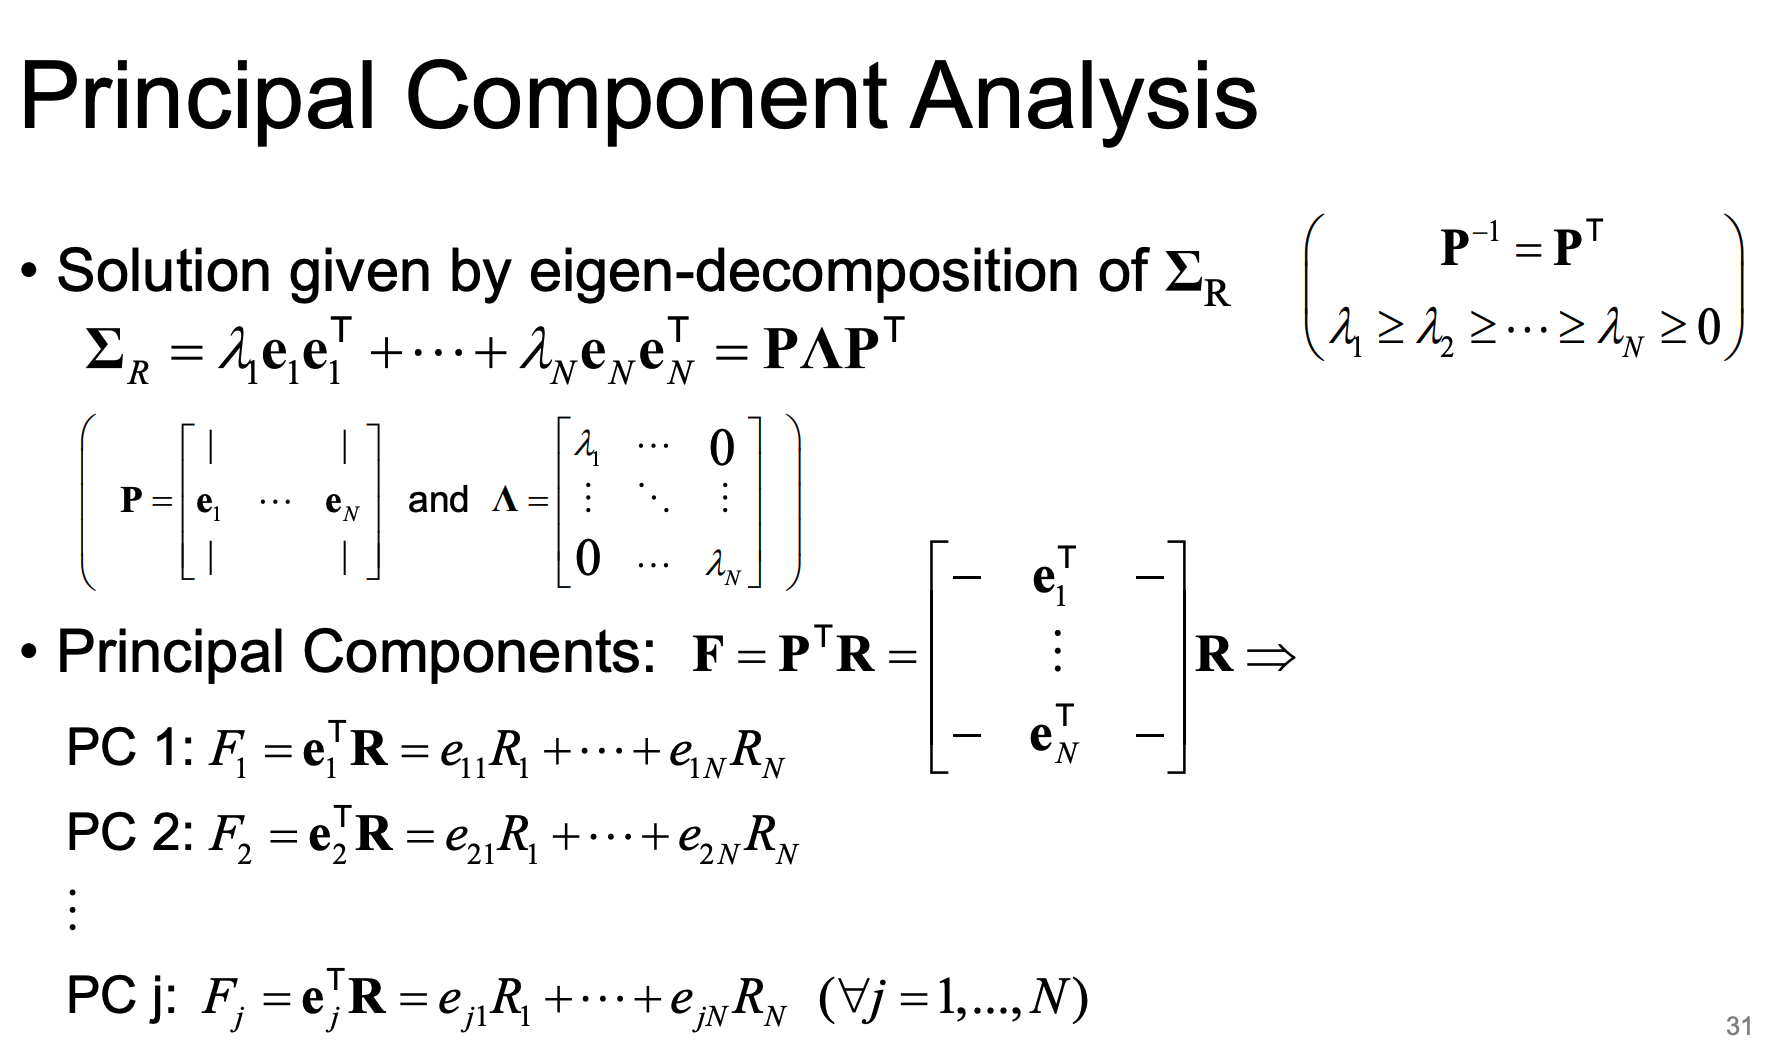
\includegraphics{Notes/Obsidian-Attachments/5-Factor-Models.png}

We can find the \(Cov(F)\) and beta (loading factor) of \(R_i\) on \(F_j\):
\[
\begin{aligned}
\mathbb{V}(\mathbf{F})&= \mathbb{V}(\mathbf{P}^{T}\mathbf{R})\\
&= \mathbf{P}^{T}\mathbb{V}(\mathbf{R})\mathbf{P}\\
&= \mathbf{P}^{T}\boldsymbol{\Sigma}_{R}\mathbf{P}\\
&\text{By Eigen-decomposition}\\
&= \mathbf{P^{T}(P\Lambda P^{T})P}\\
&\text{Where } \mathbf{P^{T}P} = 1\\
&= \boldsymbol{\Lambda}
\end{aligned} 
\]

It's kind of circular logic. Also, \(\Lambda\) is sorted with the eigenvalue associated with the eigenvector that captures the most variance is first.

\begin{quote}
Fact: Total variance of all PC's is equal to original variable variance.
\end{quote}

\[
\begin{aligned}
\text{ PC Total Variance = Population Total Variance } &\iff\\
tr(\Lambda) = tr(\Sigma) &\iff\\
\lambda_{1}+\dots+\lambda_{P} = \sigma_{1}^{2}+\dots+\sigma^{2}_{N}
\end{aligned}
\]

The proportion of total variance that is explained by each PC is:
\[
Var(PC_{j}) =\frac{\lambda_{j}}{\lambda_{1}+\lambda_{2}+\dots+\lambda_{N}} \quad \text{Where } j=1,\dots,N
\]

\hypertarget{selecting-components}{%
\subsection{Selecting Components}\label{selecting-components}}

The important part of PCA is how many components to select to capture a suitable amount of variability.

\emph{You don't need many components if the data is very correlated, and a few components may represent most of the variance in the data.}

We can also use a scree plot and pick the number of components before some ``elbow'' point.

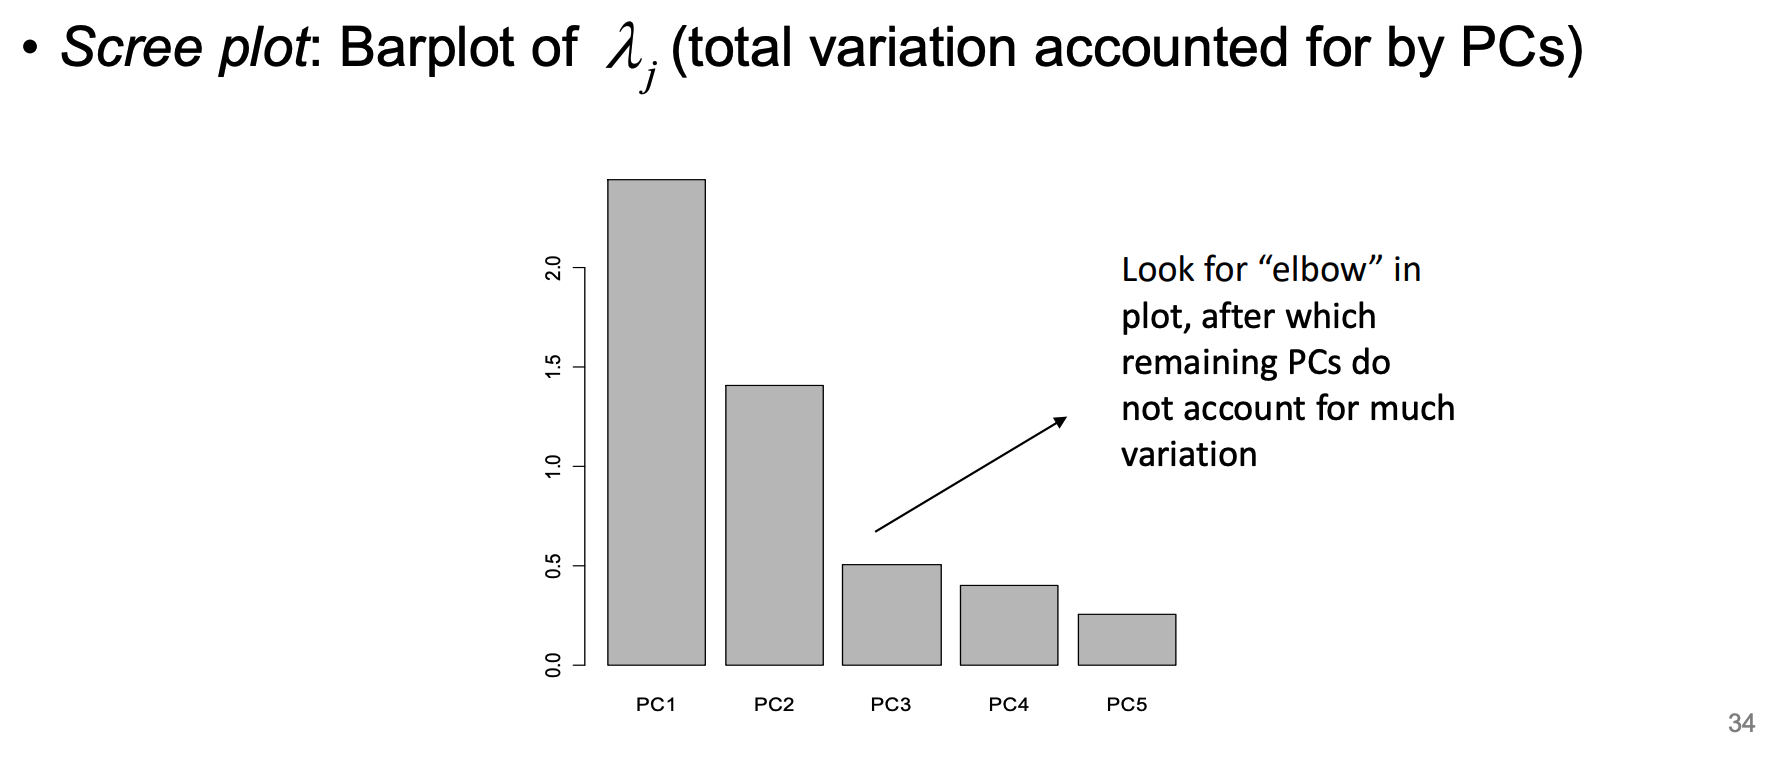
\includegraphics{Notes/Obsidian-Attachments/5-Factor-Models-1.png}

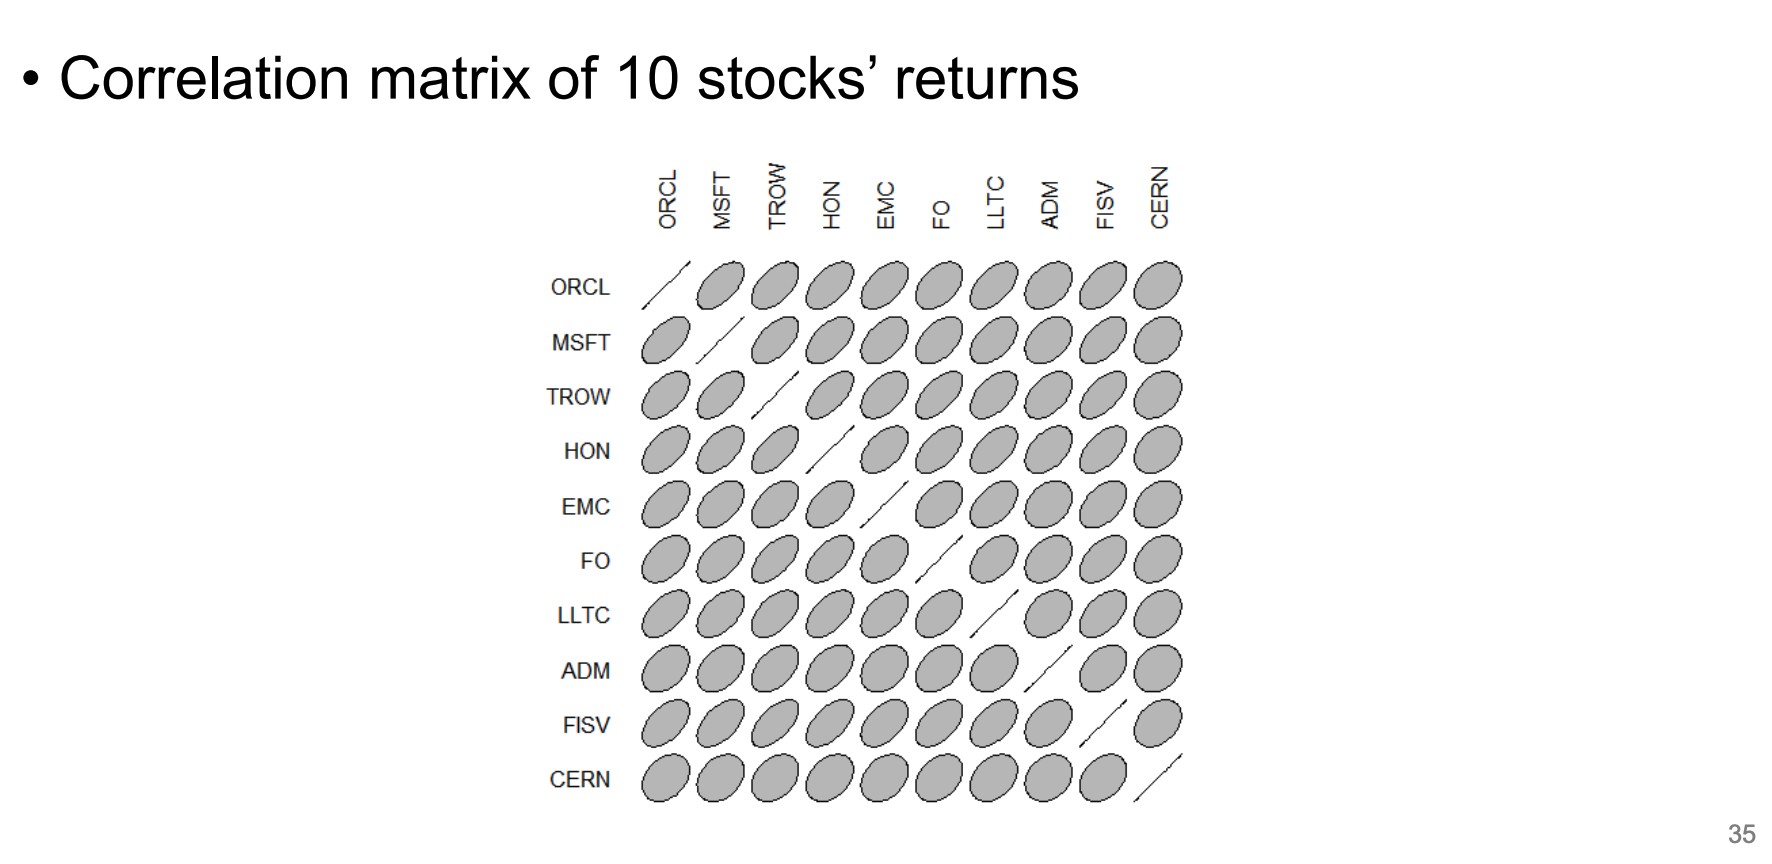
\includegraphics{Notes/Obsidian-Attachments/5-Factor-Models-2.png}

PCA run on the correlation matrix (which is the standardized covariance matrix, which is preferred when there is very large range of variances between variables)

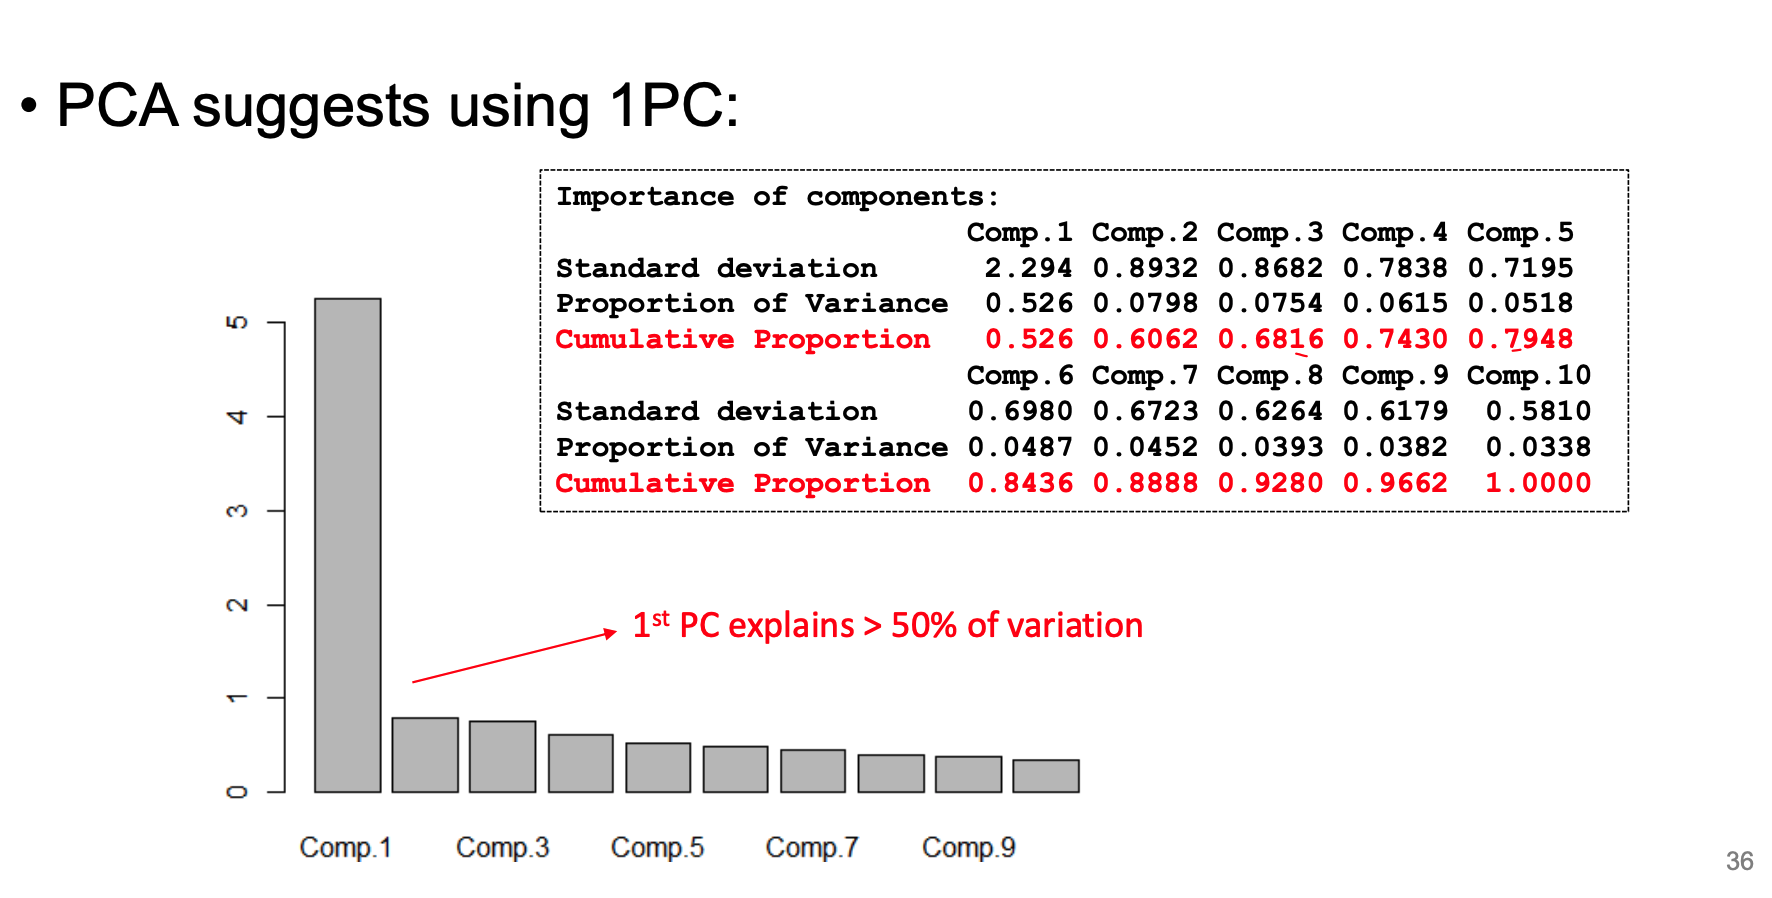
\includegraphics{Notes/Obsidian-Attachments/5-Factor-Models-3.png}

When we look at the first component, we can see it is almost an equal weighting of all the assets.

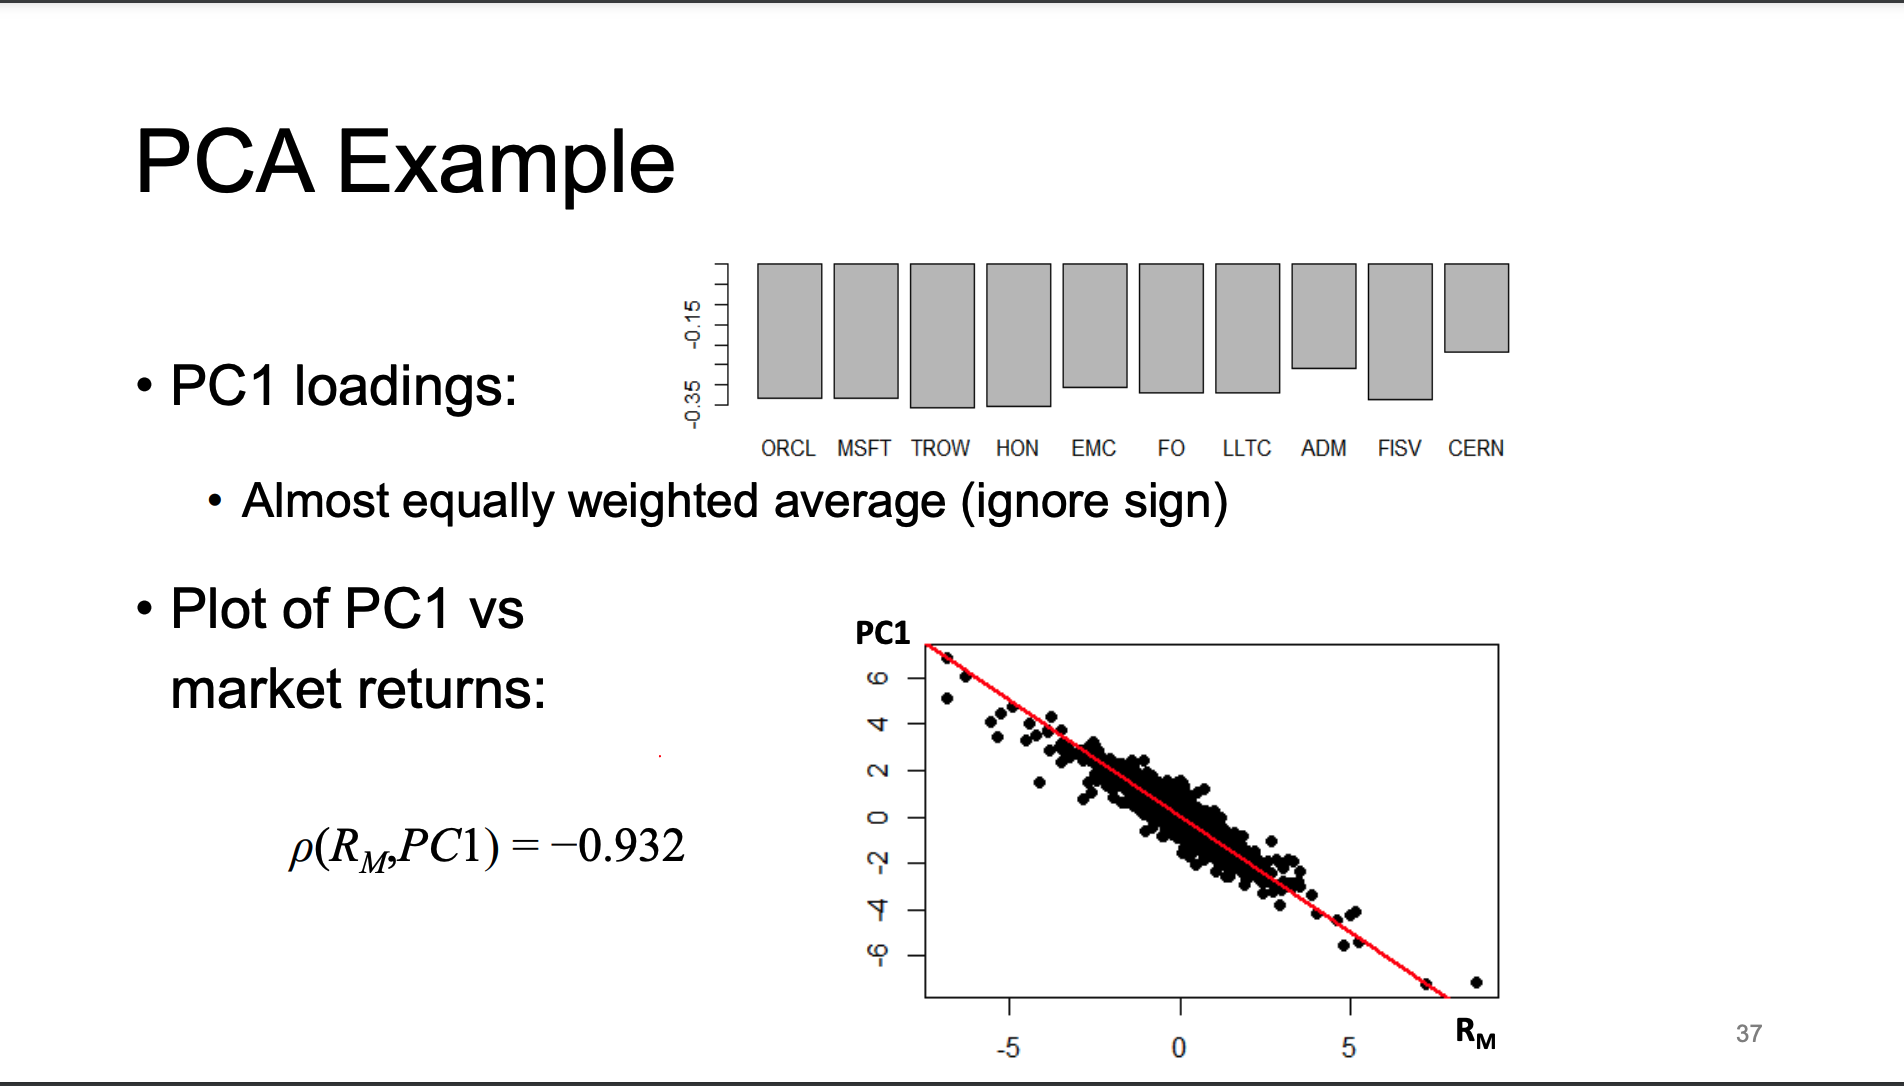
\includegraphics{Notes/Obsidian-Attachments/6-Factor-Models.png}

We can use PCA to identify components that explain overall variation of the data, although it is not guaranteed to give meaning components. For a proper data-generating model, we must use Factor Analysis.

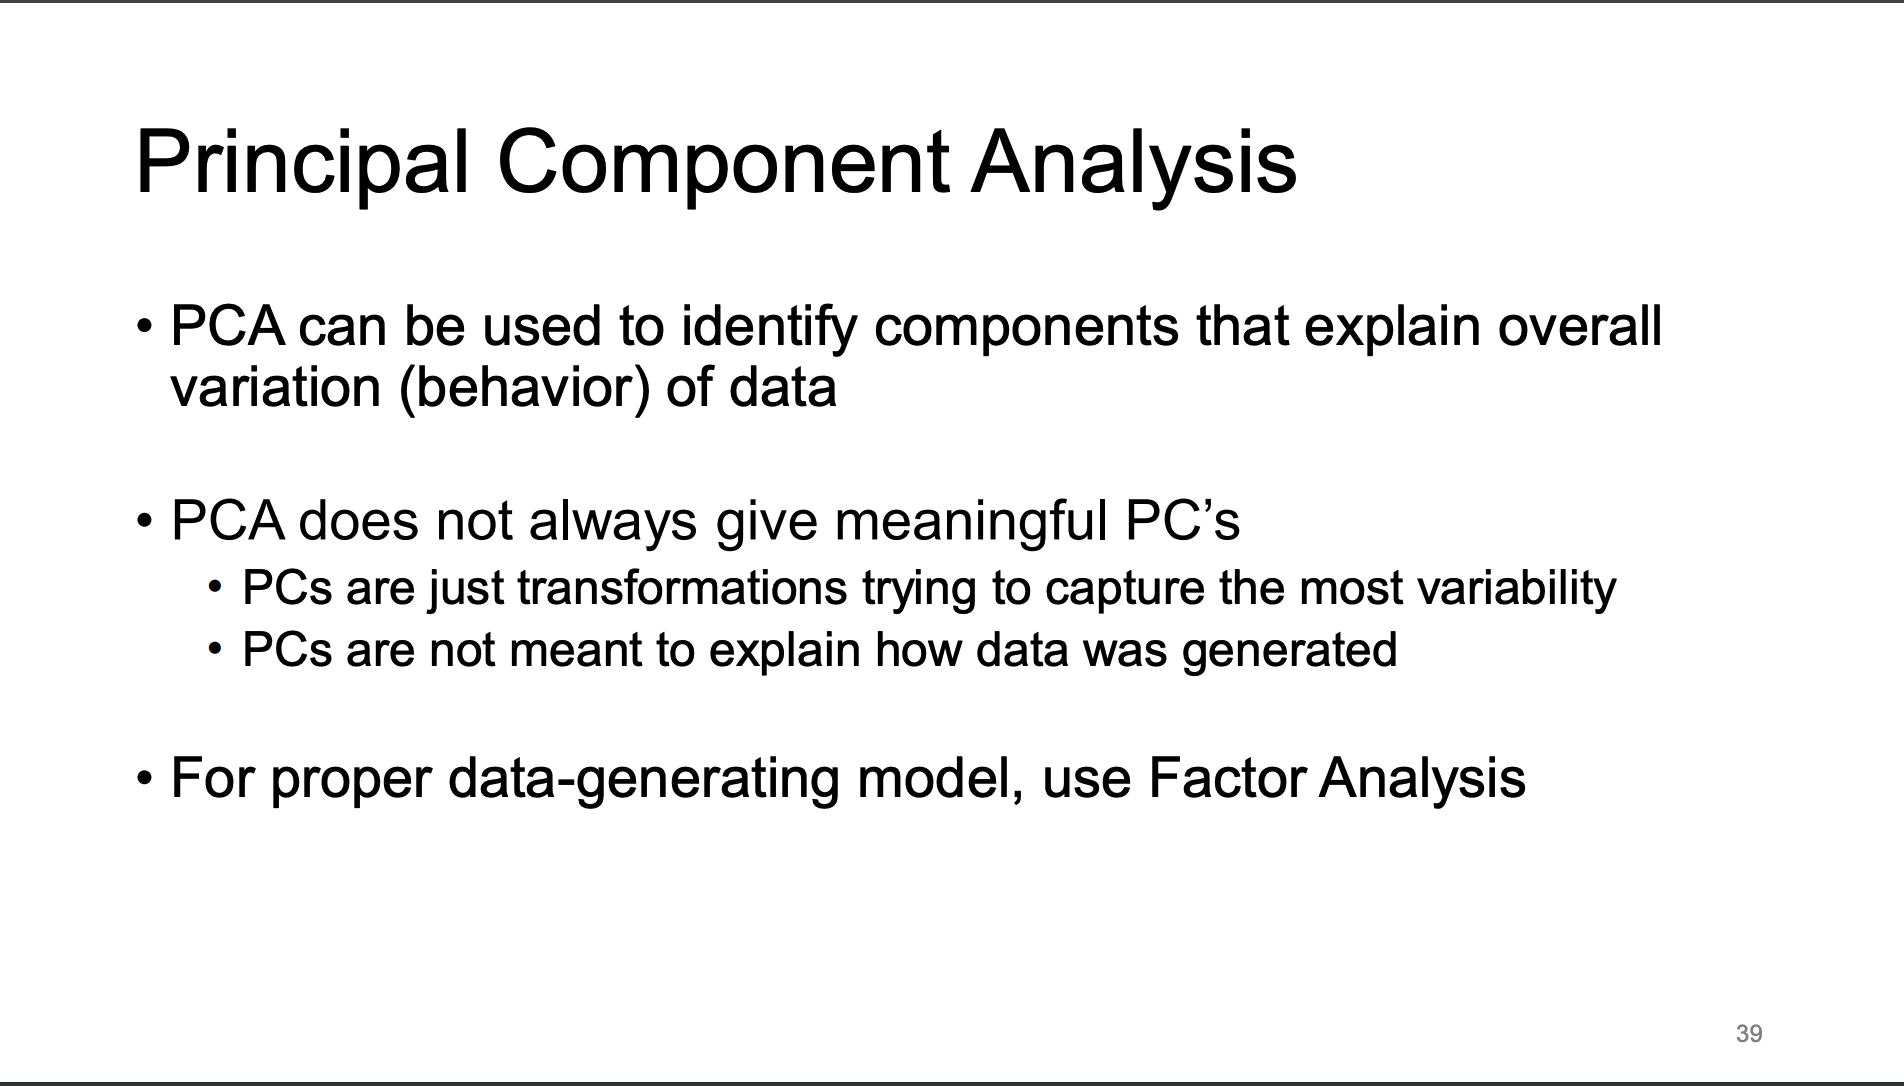
\includegraphics{Notes/Obsidian-Attachments/6-Factor-Models-1.png}

\hypertarget{factor-analysis}{%
\section{Factor Analysis}\label{factor-analysis}}

\begin{quote}
He didn't go into much detail, just went over how the factor analysis works at a high level and how you can't really try to interpret the factors.
\end{quote}

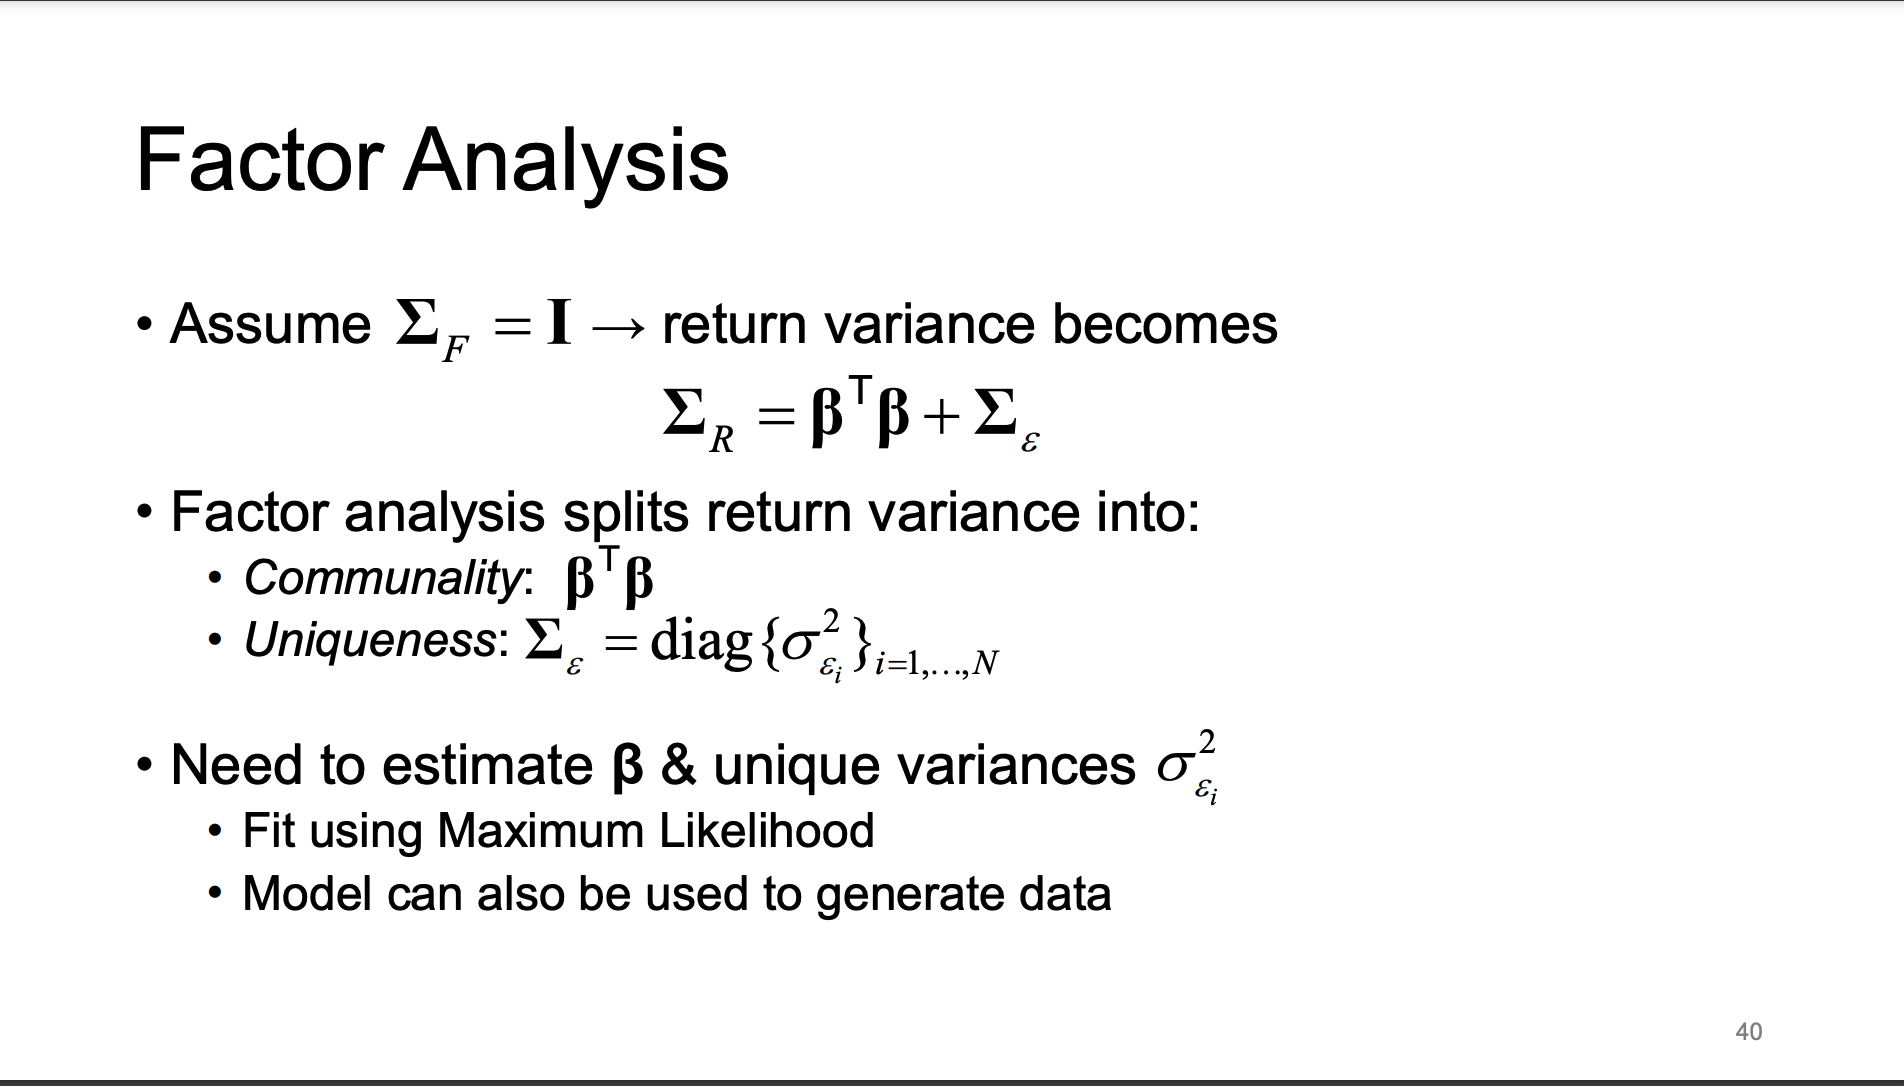
\includegraphics{Notes/Obsidian-Attachments/6-Factor-Models-2.png}

If the variance of the factors is simply the identity matrix, the variance of the returns is just the cross products of the factor variables plus some error variance.

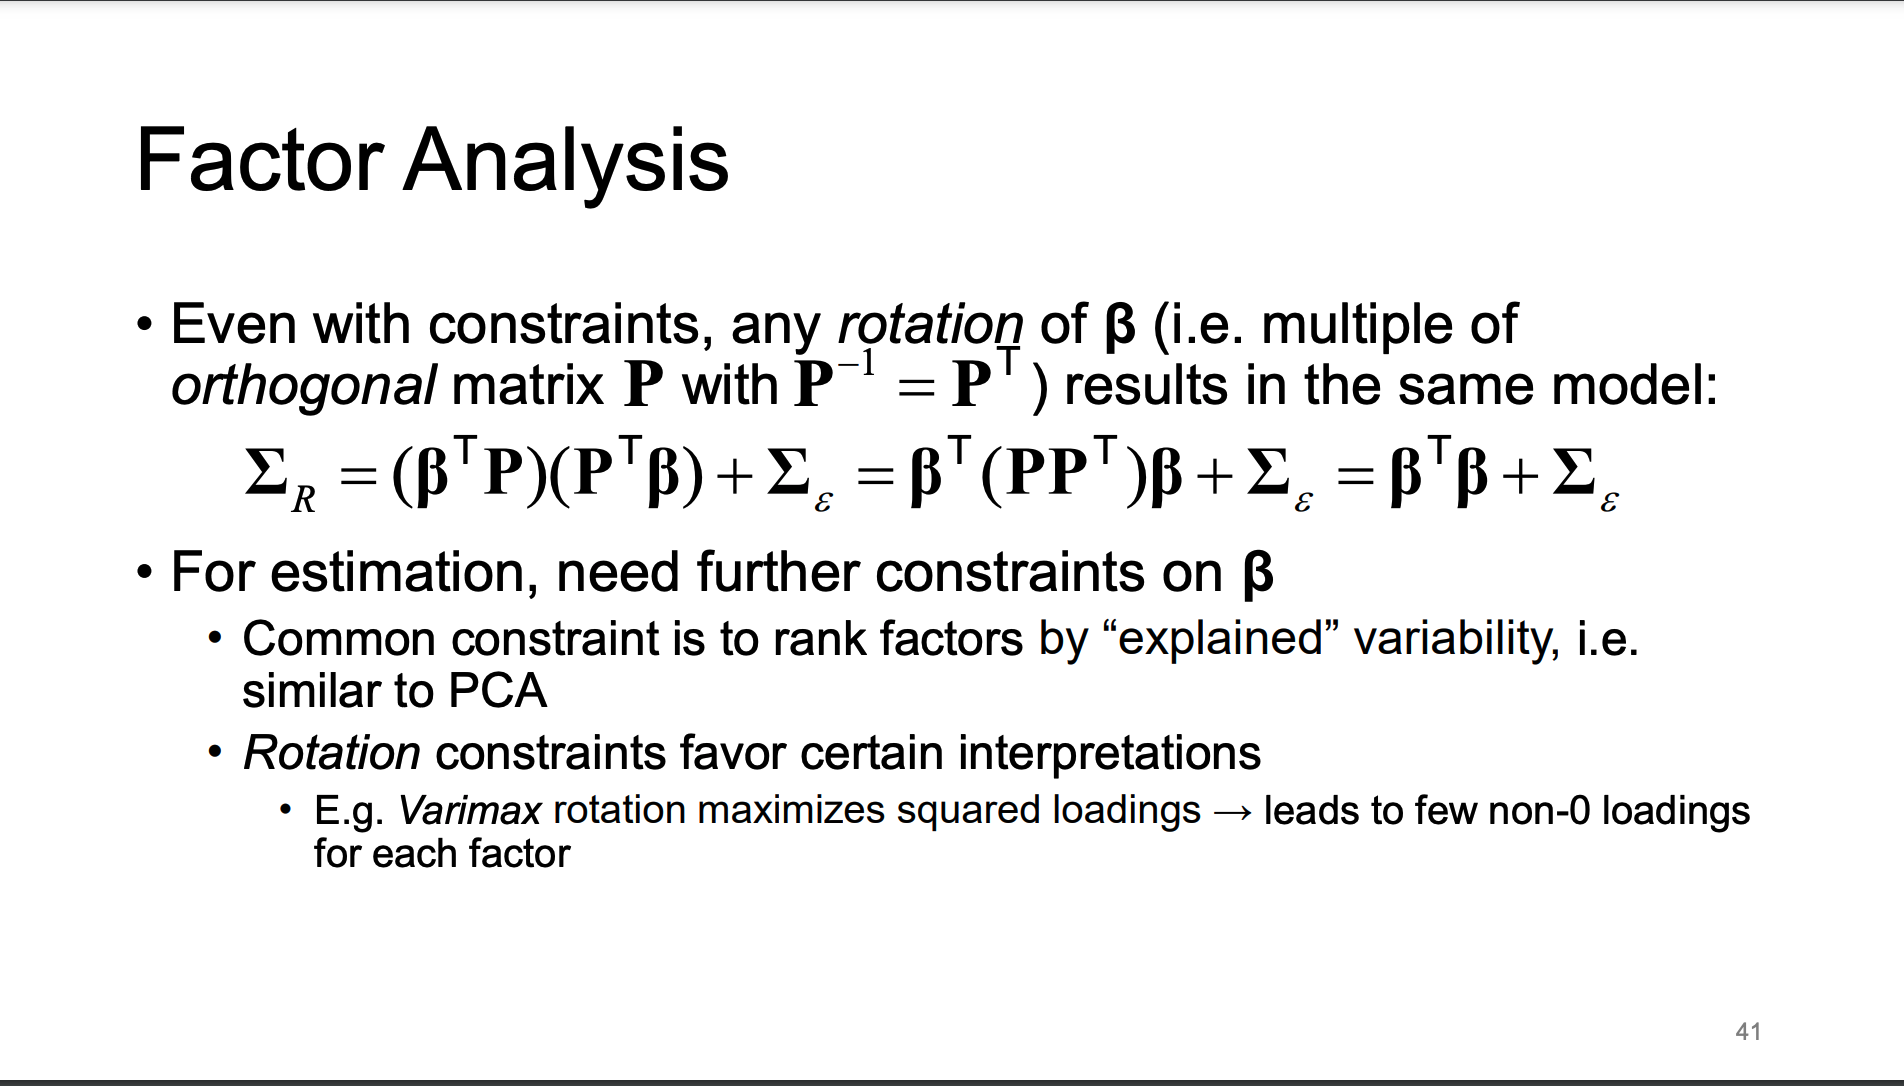
\includegraphics{Notes/Obsidian-Attachments/6-Factor-Models-3.png}

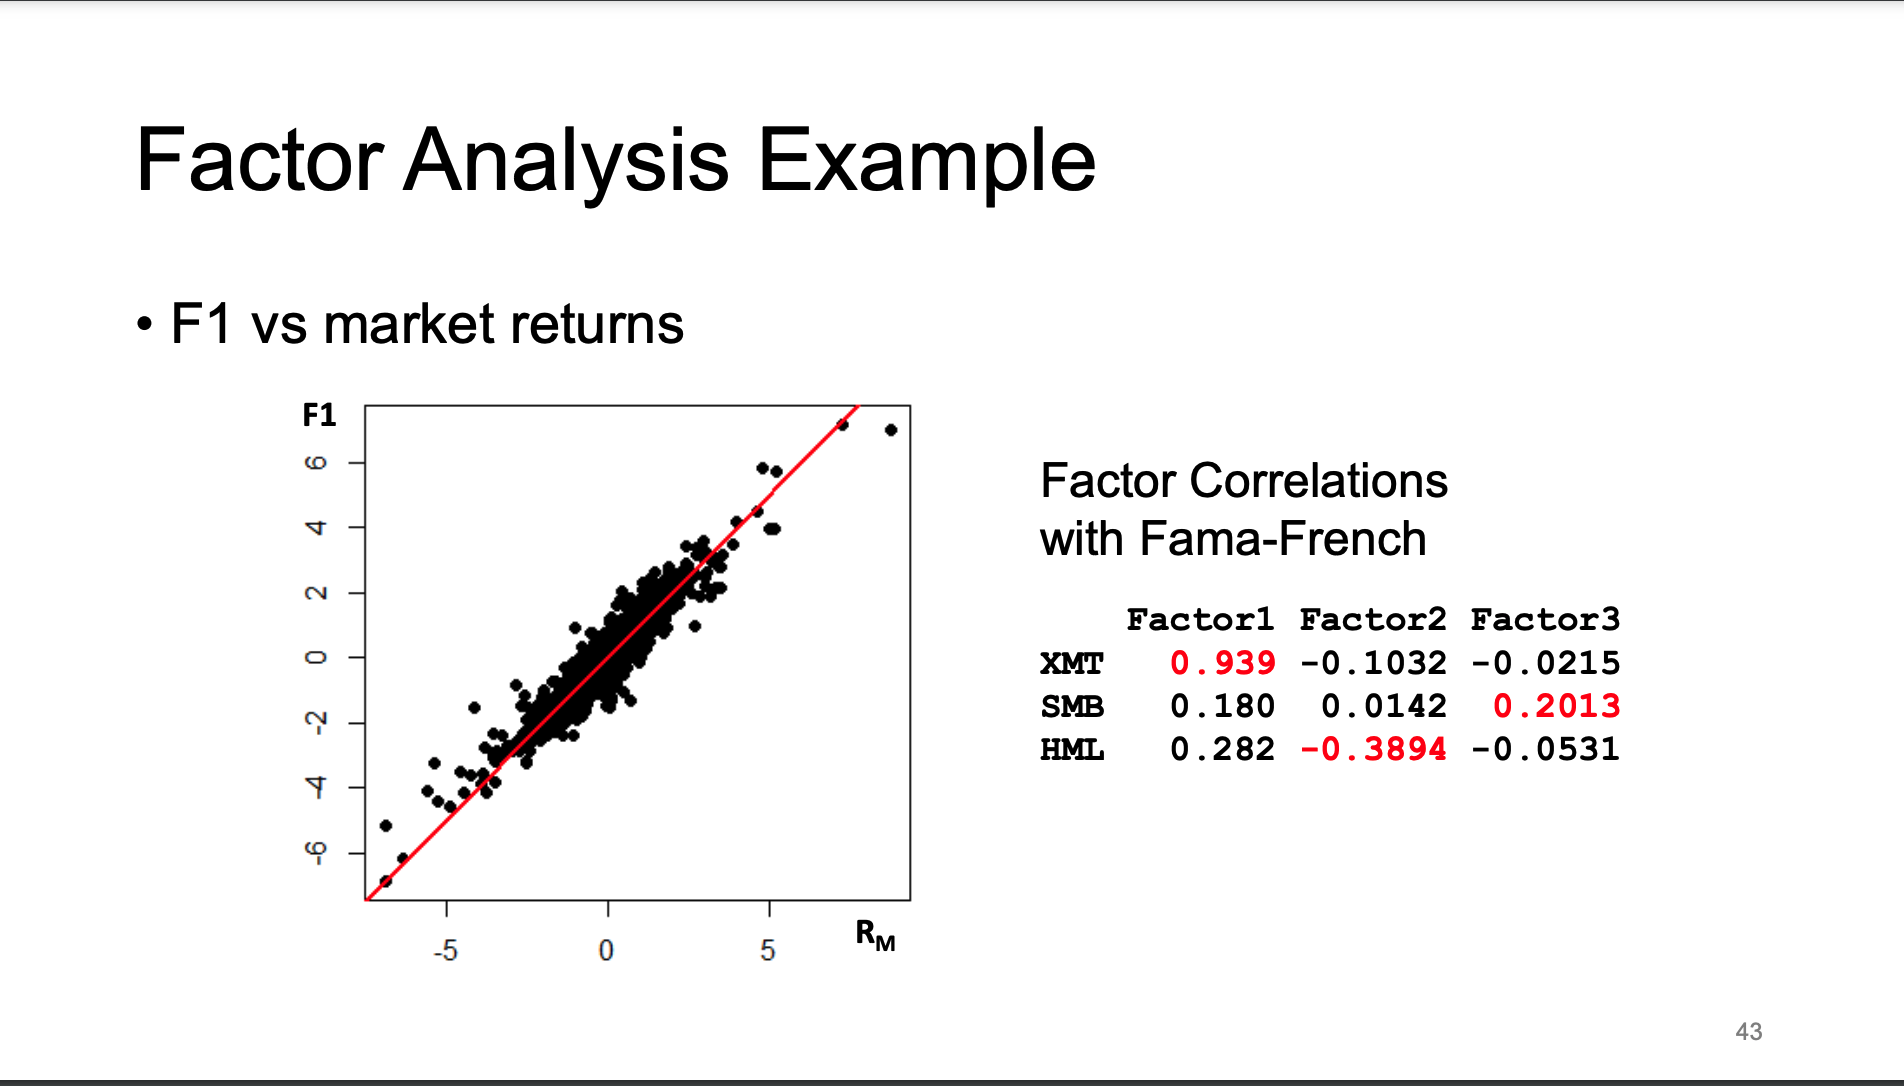
\includegraphics{Notes/Obsidian-Attachments/6-Factor-Models-4.png}

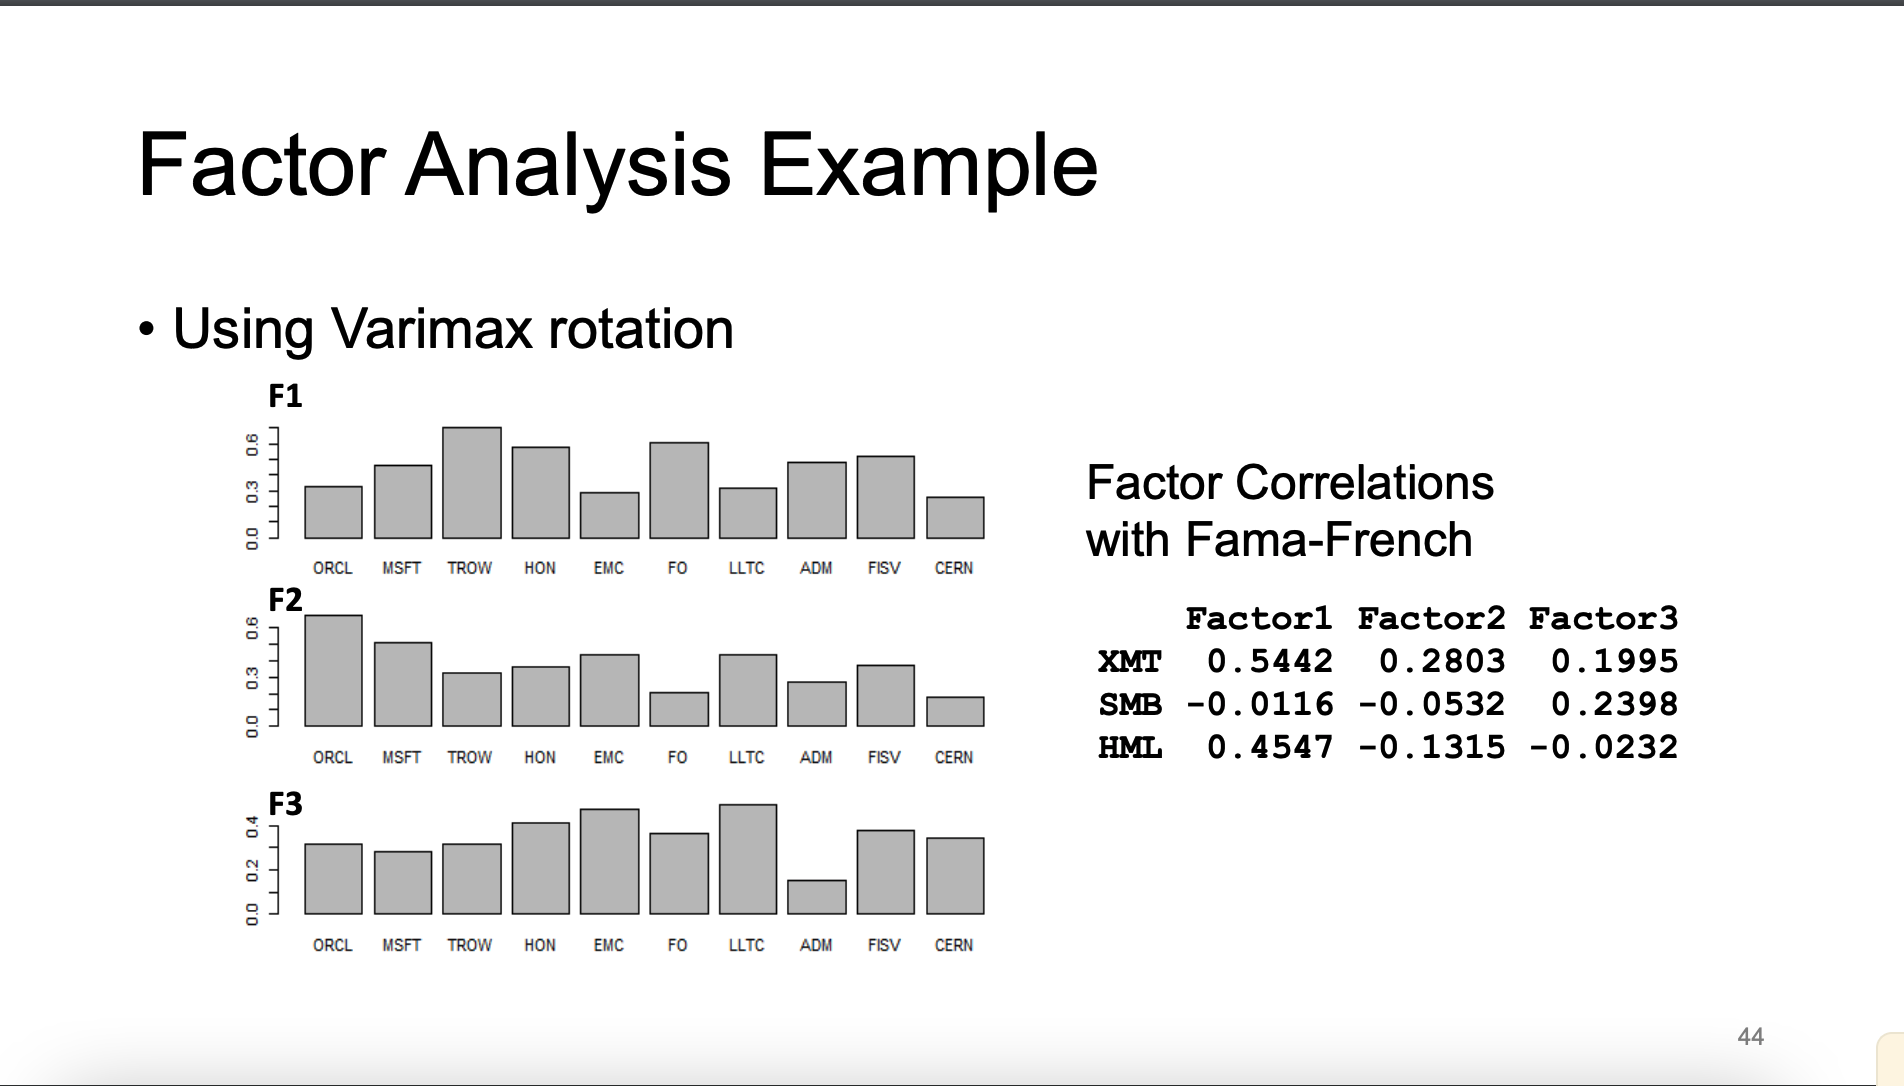
\includegraphics{Notes/Obsidian-Attachments/6-Factor-Models-5.png}

\hypertarget{risk-measures}{%
\chapter{Risk Measures}\label{risk-measures}}

We will primarily focus on market risk.

Financial risk describes the possibility of an investment losing money. It can have several sources, the main ones being:

\begin{itemize}
\tightlist
\item
  Market risk: due to changes in market prices
\item
  Credit risk: counterparty doesn't honor obligations
\item
  Liquidity risk: lack of asset tradability
\item
  Operational risk: from organization's internal activities

  \begin{itemize}
  \tightlist
  \item
    E.g., legal, fraud, or human error risk
  \end{itemize}
\item
  Risk management is the process of identifying, measuring, and controlling risk
\end{itemize}

The first thing we want to do is quantify the risk somehow.

To operationalize risk management, we use risk measures to define some capital requirement that the organization should hold in a liquid asset/cash.

The first thing that comes to mind is measuring risk by the variance of returns. \textbf{But it is not a good risk measure}. In the following example, the variances are the same, but clearly the risk is different.

WIth the left distribution, the long tail goes to the left which means your returns could become large negative values. (Reasonable to assume it is ``more risky'')

For the right distribution, the average return is negative although there is no chance of very large negative returns. (Implies that it is ``less risky'')

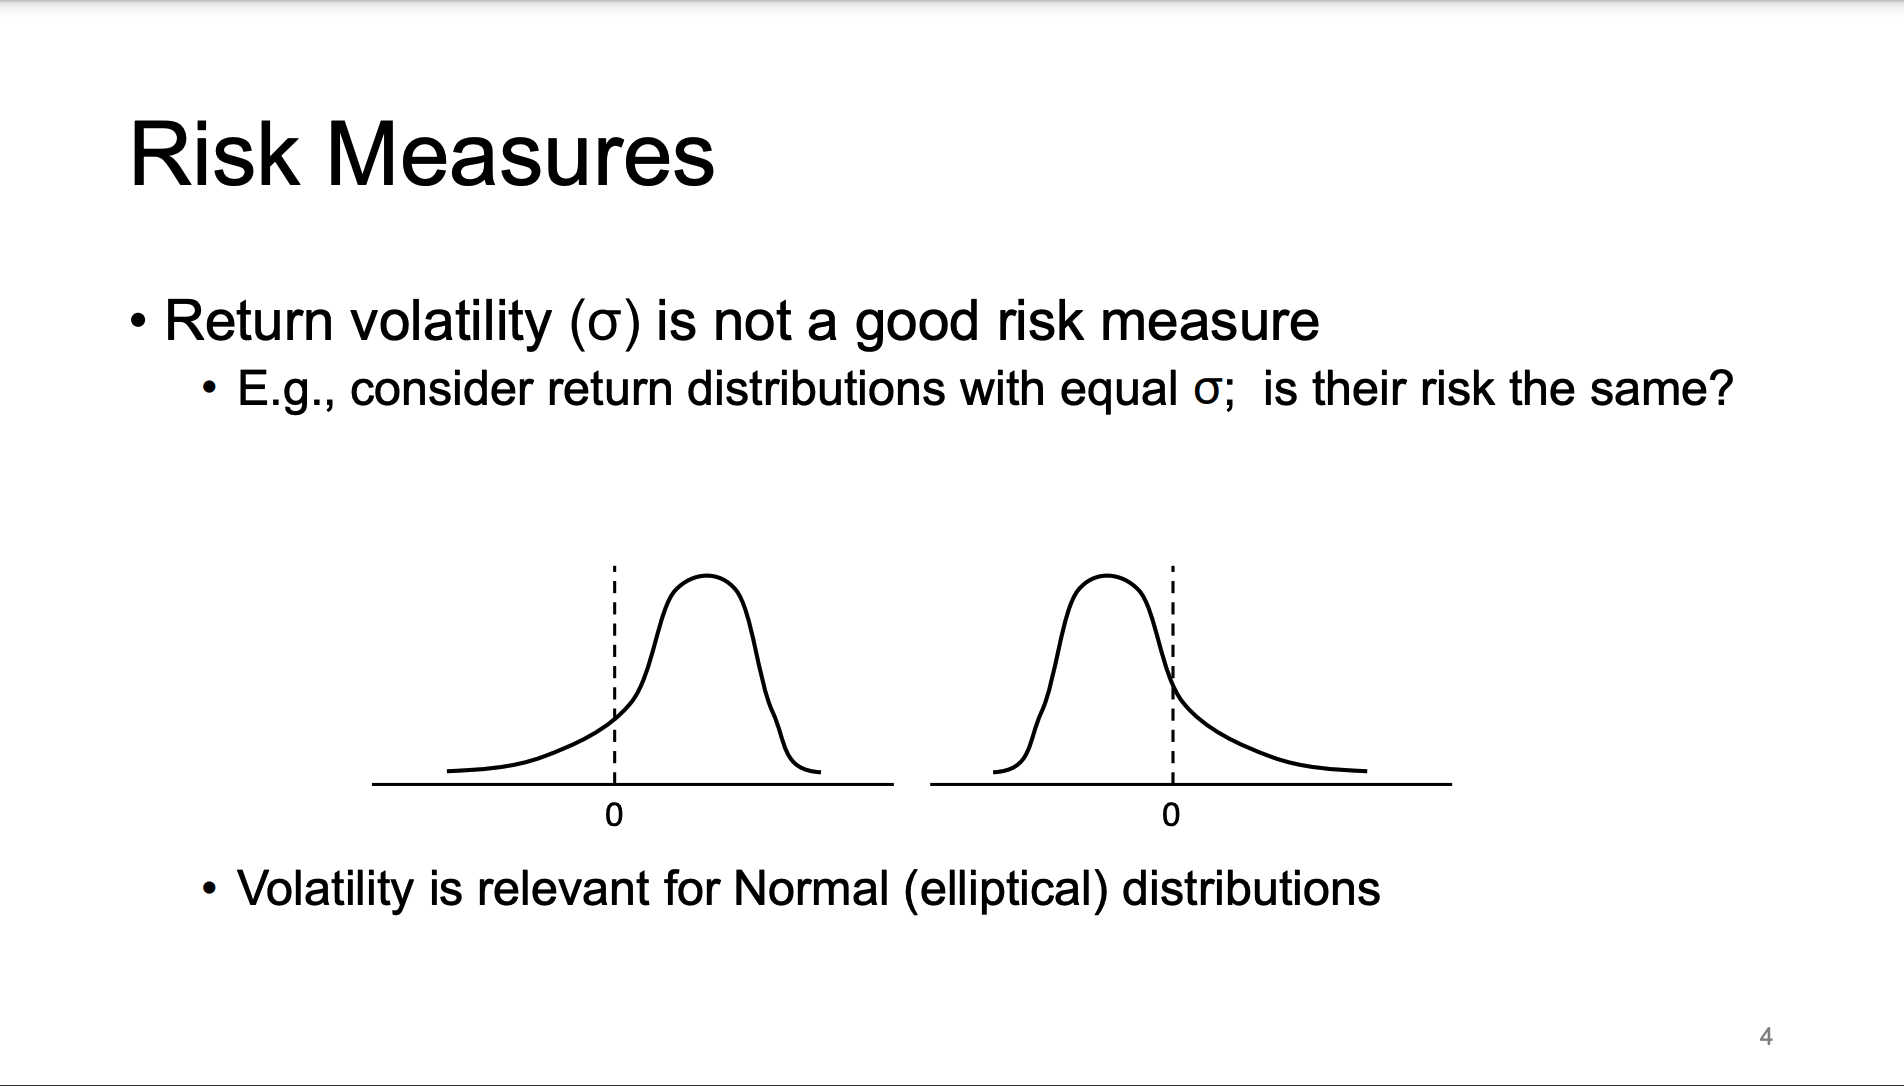
\includegraphics{Notes/Obsidian-Attachments/7-Risk-Management.png}

\begin{quote}
The point of risk mgmt: We want to know the amount of money we should set aside to cover expected losses.
\end{quote}

\hypertarget{formulas}{%
\section{Formulas}\label{formulas}}

Assuming \(Port \sim N(\mu, \sigma^{2})\)
\[
\begin{aligned}
VaR_{\alpha} &= \mu +z_{\alpha}\cdot \sigma\\
ES_{\alpha} &= \mu + \frac{\phi(z_{\alpha})}{\alpha} \cdot \sigma\\
EVaR_{\alpha} &= \mu + \sigma \cdot \sqrt{-2\ln(\alpha)}
\end{aligned}
\]

\hypertarget{value-at-risk-var}{%
\section{Value At Risk (VAR)}\label{value-at-risk-var}}

Was really common, although recently it has decreased in use (discredited) although there are variations still in use.

Let \(\mathrm{RV}\) \(L\) be the loss of an investment over some time period \(T\)

\begin{itemize}
\tightlist
\item
  Loss is negative of gain/revenue \((R): L=-R\)
\end{itemize}

\begin{quote}
We look at losses because we only capture the negative losses from this asset
\end{quote}

Value at Risk at confidence level \((1-\alpha)\) \& time horizon \(T\) is defined as the:

\textbf{\((1-\alpha)\)-quantile of \(L\) for some \(\alpha \in(0,1)\)}

\[
\begin{aligned}
\operatorname{VaR}(\alpha)=\inf \{x: P(L \leq x) \geq 1-\alpha\}=\inf \{x: P(L>x) \leq \alpha\}
\end{aligned}
\]

\begin{quote}
Infimum (smallest value of x) is only used for discrete distributions such that the the probability of \(L\) will not exceed some value \(x\) and we want this to happen \((1-\alpha)\) of the time. (Usually want it to be less than \(5\%\))
\end{quote}

\begin{itemize}
\tightlist
\item
  For continuous RV with \(\operatorname{CDF} F_L\) , we don't need the infimum anymore and can just do: \(\Rightarrow \operatorname{VaR}(\alpha)=F_L^{-1}(1-\alpha)\)
\end{itemize}

\begin{quote}
Basically the quantile of the distribution
\end{quote}

\begin{itemize}
\tightlist
\item
  VaR represents amount that covers losses with probability \((1-\alpha)\)
\end{itemize}

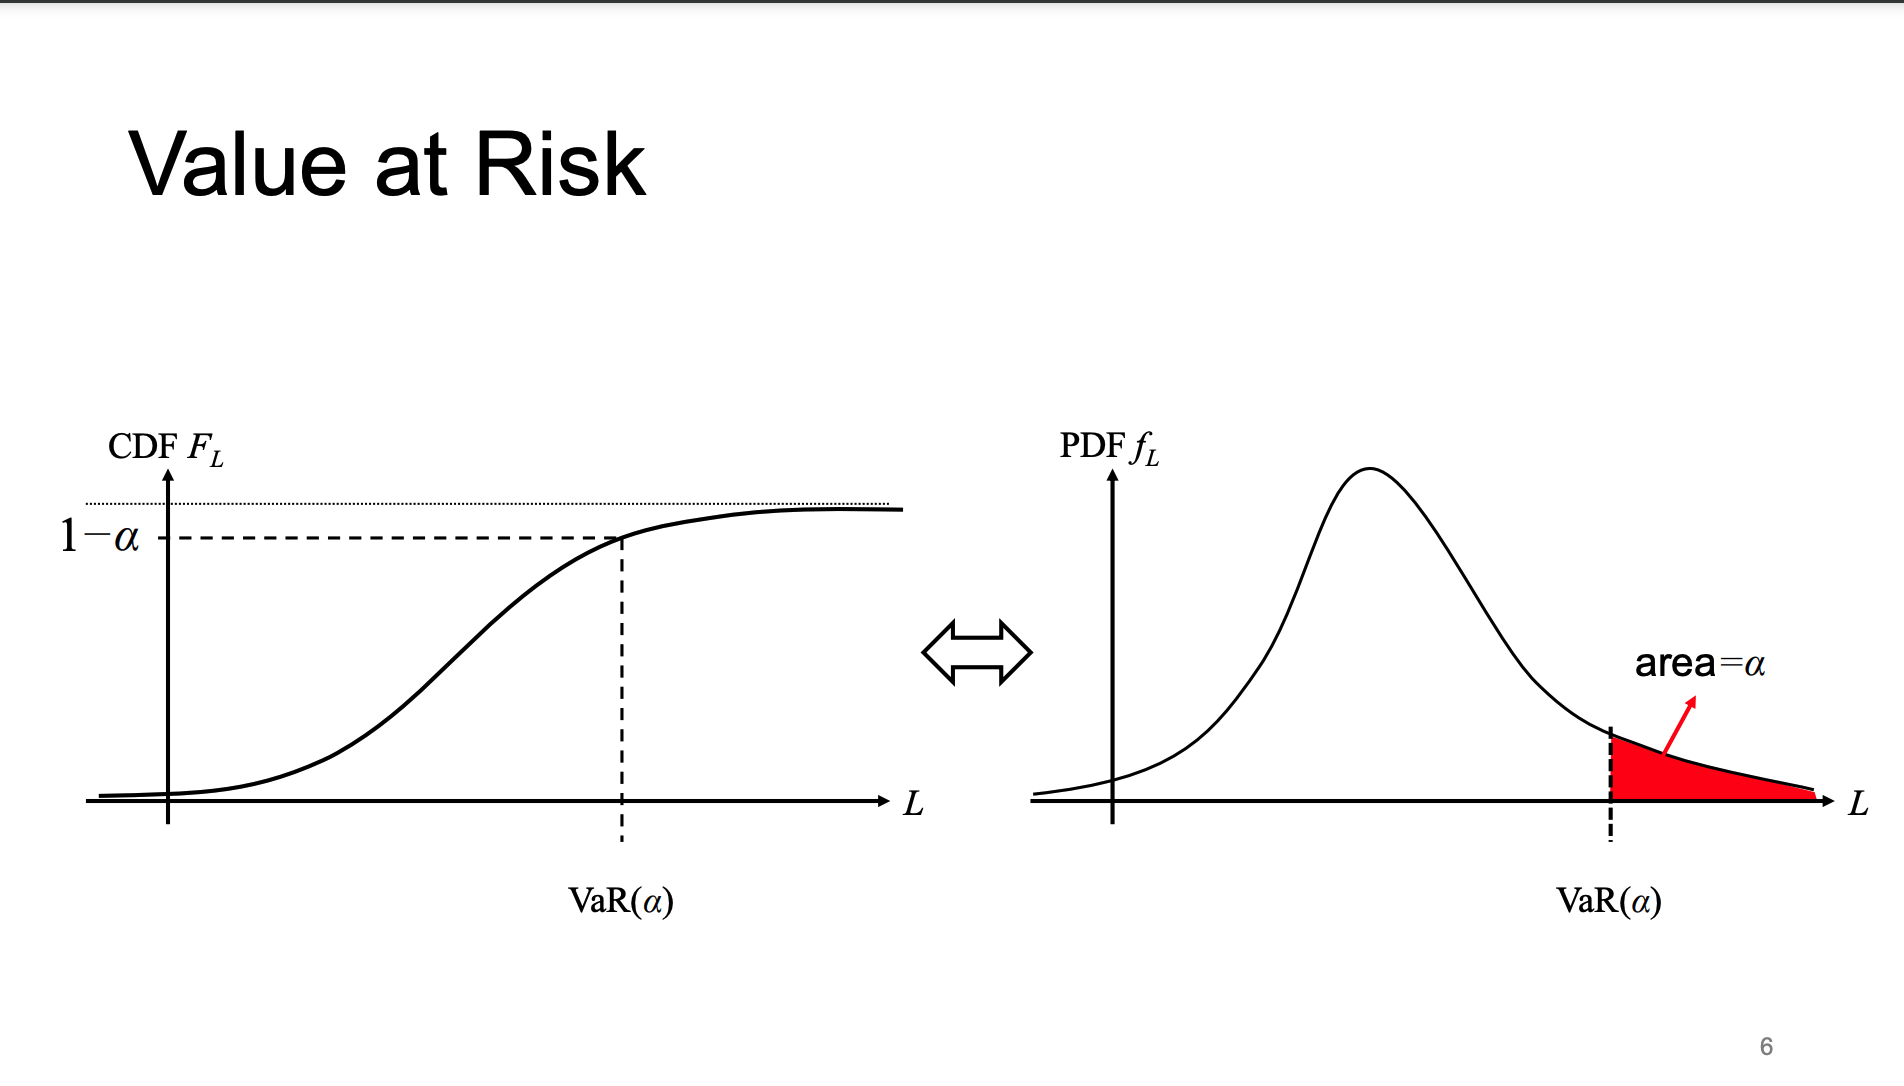
\includegraphics{Notes/Obsidian-Attachments/7-Risk-Management-1.png}

\begin{quote}
We want the quantile at which the probability is at \((1-\alpha)\)
\end{quote}

\begin{quote}
The VaR(\(\alpha\)) value indicates what value of \(x\) we need to hold to cover our losses \((1-\alpha) = 95\%\) of the time.
\end{quote}

\hypertarget{example-1}{%
\subsection{Example}\label{example-1}}

Consider asset with \(N(\mu=.03, \sigma^{2}=.04)\) annual log-returns. Find the 95\% confidence level annual VaR for a \(S_{0} =\)\$1000 investment in this asset. Let \(R=S_{T}-S_{0}\) represent revenue (-losses)

We want to find the VaR(\(\alpha\)) s.t
\[
\begin{aligned}
P(L > VaR) &= 5\%\\
&= P(-R > VaR) \\
&= P(R < -VaR)\\
\\
X &\sim N(0.03, \sigma^{2}=0.04)\\
\implies S_{T} &= S_{0}\cdot e^{X}\\
\\
P(S_{T}-S_{0} < -VaR) &= P(S_{T} < S_{0}-VaR)\\
&= P(S_{0}e^{X} < S_{0}\cdot VaR)\\
&= P\left( X < \log\left( \frac{S_{0}-VaR}{S_{0}} \right)\right)\\
&= P\left( \underbrace{ \frac{X-0.03}{.2} }_{ Z\sim N(0,1) } < \frac{\log\left( 1-\frac{VaR}{S_{0}} \right)-0.03}{.2} \right) = 0.05\\
&= P\left( Z < \underbrace{ \frac{\log\left( 1-\frac{VaR}{S_{0}} \right)-0.03}{.2} }_{ z } \right) = 0.05\\
\implies z &= -1.645\\
\frac{\log\left( 1-\frac{VaR}{S_{0}} \right)-0.03}{.2} &= -1.645\\
\\
\mathbf{VaR} &= (1-\exp\{-1.645\cdot 0.20+0.03\}) \cdot S_{0}\\
\mathbf{VaR} &= (1-\exp\{-0.299\})\cdot 1000\\
&= \mathbf{258.44}
\end{aligned}
\]

VaR is basic and widely used as a risk measure to simply indicate

\begin{quote}
\emph{``What is the most I can lose on this investment?''}
\end{quote}

It has been widely used partly because of the Basel framework which is some risk management standard for banks and banks implemented Basel to comply.

However it has some glaring issues. No one trusts it as a proper risk management tool.

Flaws:
- VaR hides tail risk (hides risk of very extreme events) although there is a way to remedy it
- It discourages diversification

The additional resources talk about why VaR is not a good measure of risk:
{[}{[}../../Lectures/Risk Mismanagement.pdf{]}{]}
{[}{[}../../Lectures/Against VaR.pdf{]}{]}

\hypertarget{var-hides-tail-risk}{%
\section{VaR hides tail risk}\label{var-hides-tail-risk}}

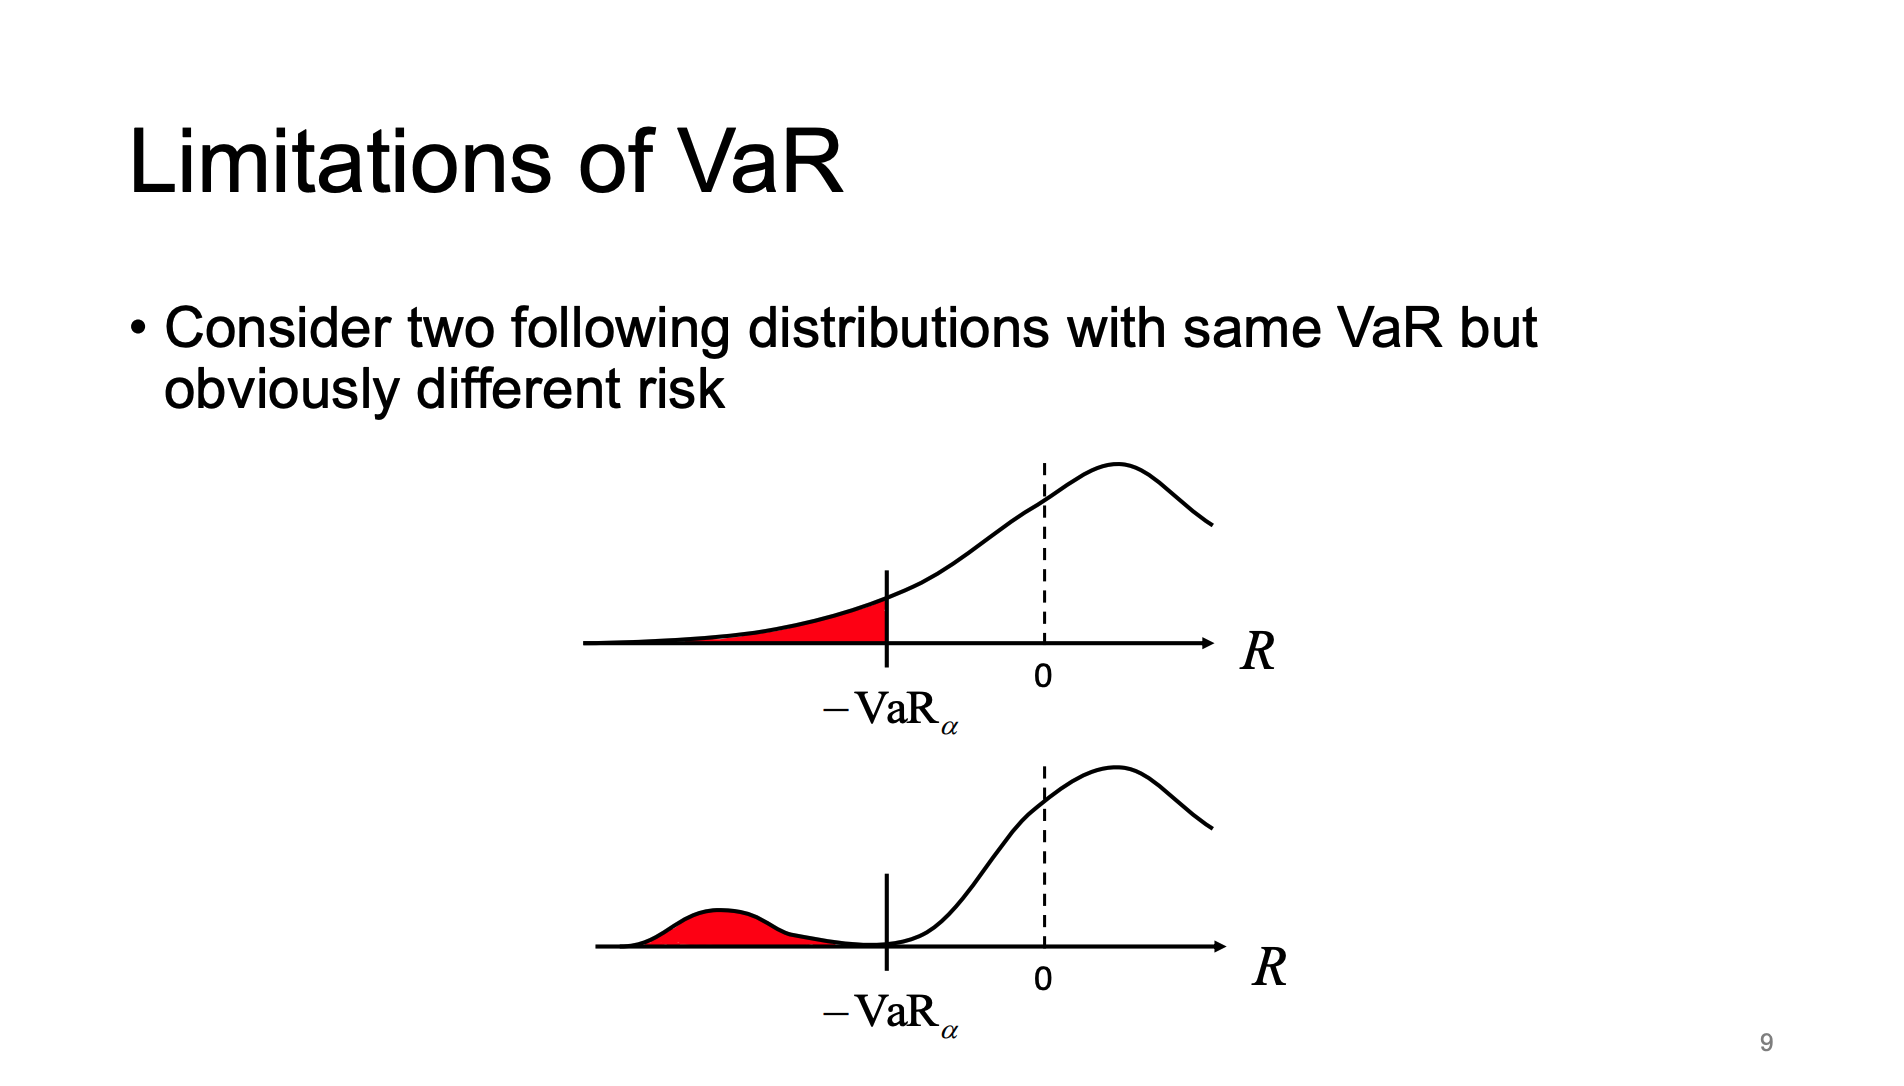
\includegraphics{Notes/Obsidian-Attachments/7-Risk-Management-2.png}

Var doesn't care what happens beyond the cut off, just the actual z-score (or whatever score from some distribution). If we push some density of losses very far (hiding a small probability of really bad events), we can actually concentrate the density of profits higher.

\hypertarget{mitigation-cond-var-or-expected-shortfall}{%
\subsubsection{Mitigation: Cond VaR or Expected Shortfall}\label{mitigation-cond-var-or-expected-shortfall}}

AKA CVar or ES

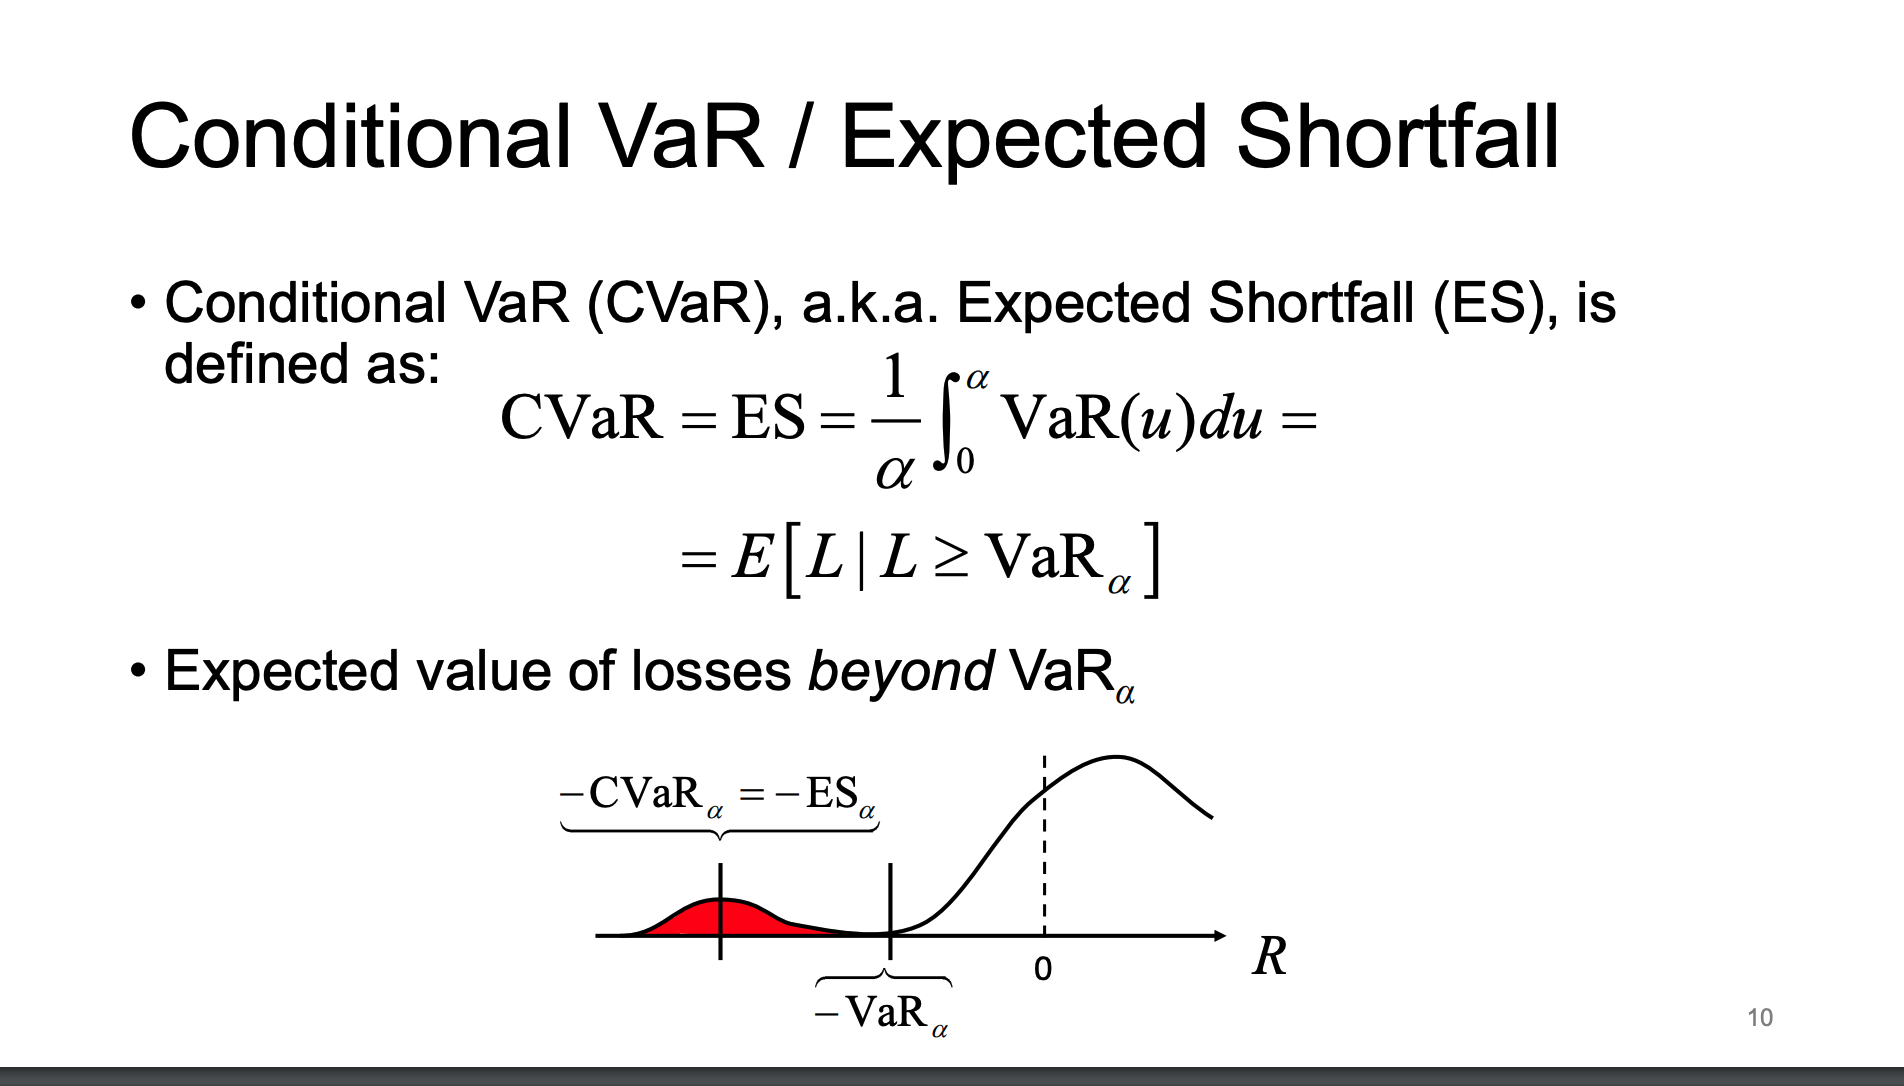
\includegraphics{Notes/Obsidian-Attachments/7-Risk-Management-3.png}

This gives us the expected losses that can occur given that we are beyond \(VaR_{\alpha}\)

\begin{quote}
Imagine we cut off the loss distribution beyond the VaR(\(\alpha\))\(=x\) point, and we have another little distribution of losses which are way larger/further from the bulk of the distribution.
We take the mean/average/expected value of this distribution which tells us ``hey in the 5\% scenario our losses are so huge, what can we \textbf{expect} to lose?''
\end{quote}

\hypertarget{example-2}{%
\subsubsection{Example}\label{example-2}}

If \(R\sim N(0,1)\), find ES at confidence level \(\alpha\)

\[
\begin{aligned}
R\sim N(0,1) &\implies L \sim N(0,1)\\
\text{Let } Z_{\alpha} &\text{denote the } \alpha \text{-quantile of the std normal}\\
\\
ES_{\alpha} &= \mathbb{E}[L|L>Z_{\alpha}] = \int ^{\infty}_{Z_{\alpha}} x \ \phi(x| L> z_{\alpha}) \, dx\\
&= \int ^{\infty}_{Z_{\alpha}} x \frac{\phi(x)}{\underbrace{ P(L > Z_{\alpha}) }_{ \alpha }}\, dx \\
&= \frac{1}{\alpha}\int ^{\infty}_{Z_{\alpha}} x \frac{1}{2\sqrt{ \pi }}e^{-x^{2}/2}\, dx \\
&= \frac{1}{\alpha}  \int ^{\infty}_{Z_{\alpha}}\frac{1}{2\pi} \lfloor-e^{-x^{2}/2}\rfloor  \, dx \\
&= \frac{1}{\alpha} \frac{1}{2\pi} \left[-e^{-x^{2}/2}\right]^{\infty}_{x=z_{\alpha}}\\
\implies ES_{\alpha} &= CVaR_{\alpha} = \frac{1}{\alpha}\frac{1}{\sqrt{ 2\pi }}e^{-z_{\alpha}^{2}/2}\\
&= \frac{1}{\alpha} \phi(z_{\alpha})
\end{aligned}
\]

This means that generally for \(L\sim N(\mu, \sigma^{2})\),
\[
\begin{aligned}
ES_{\alpha} &= \mu + \frac{\phi(z_{\alpha})}{\alpha} \cdot \sigma\\
VaR_{\alpha} &= \mu +z_{\alpha}\cdot \sigma
\end{aligned}
\]

and for small \(\alpha\), \(\frac{\phi(z_{\alpha})}{\alpha} > z_{a}\) which implies \(ES_{\alpha}\geq VaR_{\alpha}\)

\hypertarget{risk-measure-properties}{%
\section{Risk Measure Properties}\label{risk-measure-properties}}

We now look at formal set of requirements for risk measures (5 properties)

We let \(\rho(L)\) represent the risk measure, which takes in a distribution of a some returns and outputs a number indicating the capital requirements (money to be kept aside) should be.
We let \(L\) is a random variable and let \(\rho\) is a functional distribution of \(L\).

For this measure \(\rho\) to reasonably quantify risk, it must:

\begin{enumerate}
\def\labelenumi{\arabic{enumi}.}
\tightlist
\item
  be normalized \(\rho(0)=0\) (risk of holding no assets is 0)
\item
  Translation invariance: \(\rho(L+c) = \rho(L) + c \ \forall c \in \mathbb{R}\)

  \begin{itemize}
  \tightlist
  \item
    adding a loss \(c\) to the portfolio increases risk by exactly \(c\)
  \end{itemize}
\item
  Positive Homogeneity: \(\rho(bL) = b\rho(l)\)

  \begin{itemize}
  \tightlist
  \item
    scaling portfolio returns also will scale risk
  \end{itemize}
\item
  Monotonicity: \(L_{1}\geq L_{2} \implies \rho(L_{1}) \geq \rho(L_{2})\)

  \begin{itemize}
  \tightlist
  \item
    The ordering of the random variables is almost surely \(P(L_{1}\geq L_{2})=1\)
  \end{itemize}
\item
  Sub-additivity: \(\rho(L_{1}+L_{2}) \leq \rho(L_{1}+L_{2})\)

  \begin{itemize}
  \tightlist
  \item
    Only when the two losses are perfectly correlated, then equal
  \item
    The risk of two combined portfolios cannot exceed the sum of the two portfolio risks
  \end{itemize}
\end{enumerate}

If a risk measure has all 5 properties, then it is called a \textbf{coherent risk measure}.

\hypertarget{example-that-var-and-cvar-satisfy-prop-2-3}{%
\subsection{Example that VAR and CVar satisfy prop 2 \& 3}\label{example-that-var-and-cvar-satisfy-prop-2-3}}

We first show that VAR and CVaR satisfy the second and third property of translation invariance and positive homogeneity.

\[
\begin{aligned}
VaR_{\alpha}(L) &= inf\{x:P(L>x) \leq \alpha\}\\
\\
\text{Let}\ \ L' &= bL+c\\
\implies VaR(L') &= inf\{x': P(L' >x') \leq \alpha\}\\
&= inf\{x':\mathbb{P}(bL+c > x') \leq \alpha\}\\
&= inf\left\{ x': \mathbb{P}\left( L> \frac{x'-c}{b} \leq \alpha \right) \right\}\\
&= inf\{bx+c : \mathbb{P}(L > x) \leq \alpha\}\\
&=b\cdot inf\{x: \mathbb{P}(L > x) \leq \alpha\}+c\\
&= b VaR(L)+c
\end{aligned}
\]
\[
\begin{aligned}
CVaR_{\alpha}(L) &= \frac{1}{\alpha}\int ^{\alpha}_{0} VaR_{u}(L) \, du\\
\implies CVaR_{\alpha}(L') &= \frac{1}{\alpha}\int ^{\alpha}_{0}(bVaR_{u}(L)+c) \, du\\
&= b\left( \frac{1}{\alpha} \int ^{\alpha}_{0}VaR_{u}(L) \, du\right) +c\\
&= b \cdot CVaR_{\alpha}(L)+c
\end{aligned}
\]

We will show that VaR is not sub-additive

Consider two risky zero-coupon bonds priced at \$95 per \$100 face value. If each one has 4\% independent default probability, show that \(VaR_{5\%}\) is not sub-additive

\[
\begin{aligned}
\text{Distribution of }L_{1/2} &= \begin{cases}
-5 & w.p. 96\% \\
+95  & w.p. 4\%
\end{cases}\\
\text{By definitioin, VaR} & = inf\{x: \mathbb{P}(L >x)<5\%\}\\
&= inf(x: \mathbb{P}(L \leq x)\geq 95\%)\\
\implies VaR_{5\%}(L_{1/2}) &= -5 \\
\end{aligned}
\]

As -5 is the smallest value that satisfies \(\mathbb{P}(L\leq x) \geq 95\%\) as \(\mathbb{P}(L \leq -5) = 96\%\)

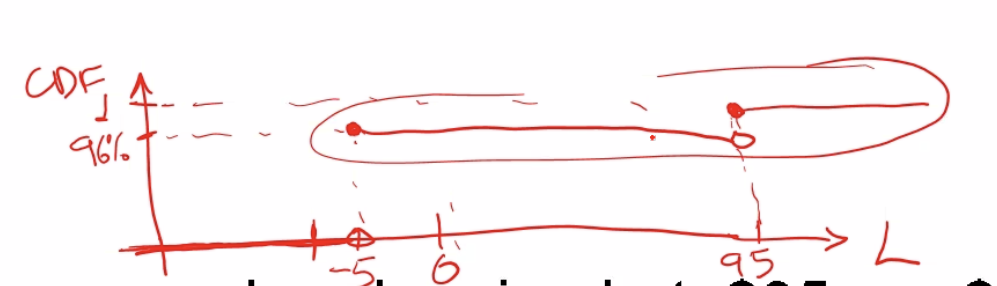
\includegraphics{Notes/Obsidian-Attachments/7-Risk-Management-4.png}

\[
\begin{aligned}
\text{Distribution of }L_{1} + L_{2} &= \begin{cases}
-5-5 = -10 \quad w.p. 96\%^{2}=92.16\% & \text{when both don't default}\\
-5+95 = 90 \quad w.p. 96\% \cdot 4\% = 7.68\% & \text{when only one defaults} \\
95+95=190 \quad w.p. 4\%^{2}=.16\% & \text{both default}
\end{cases}\\
VaR_{5\%} (L_{1}+L_{2}) &= inf\{x:\mathbb{P}(L_{1}+L_{2} < x) \geq 95\%\} = 90
\end{aligned}
\]

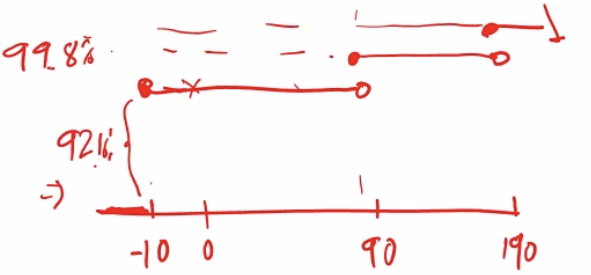
\includegraphics{Notes/Obsidian-Attachments/7-Risk-Management-7.png}

\[
\begin{aligned}
\implies VaR_{5\%}(L_{1}+L_{2}) = 90 > VaR_{5\%}(L_{1}) + VaR_{5\%}(L_{2}) = -5 -5 = 10
\end{aligned}
\]

Which suggests holding both bonds is more risky than holding them separately.

We can show that CVaR is sub-additive.

\[
\begin{aligned}
CVaR_{5\%}(L_{1}) &= \frac{1}{\alpha}\int ^{\alpha}_{0}VaR_{u}(L_{1}) \, du\\
&= \frac{1}{5\%} (95\cdot 4\% + (-5)\cdot 1\%) = 73\%\\
CVaR_{5\%}(L_{1}+L_{2}) &= \frac{1}{5\%}\int ^{5\%}_{0}VaR_{u}(L_{1}+L_{2}) \, du\\
&= \frac{1}{5\%}[190\cdot.16\%+90\cdot 4.84\%] = 93.2\\
\\
\implies CVaR_{5\%}(L_{1}+L_{2}) &= 93.2 \leq CVaR_{5\%}(L_{1})+CVaR_{5\%}(L_{2})\\
&= 2\cdot 73 = 146
\end{aligned}
\]

\hypertarget{entropic-var}{%
\section{Entropic VaR}\label{entropic-var}}

A coherent alternative to VaR based on the Chernoff bound for tail probability

For positive RV \(X\), the Chernoff inequality gives:
\[
P(X\geq c) \leq \frac{\mathbb{E}(x)}{c} \quad \forall c > 0
\]
For loss RV \(L\) with mgf \(M_L(z)=E\left[e^{z L}\right]<\infty, \forall z>0\) we have \(P(L \geq c) \Leftrightarrow P\left(e^{z L} \geq e^{z c}\right) \leq M_L(z) e^{-z c}\) Limiting bound to \(M_L(z) e^{-z c} \leq \alpha\) and solving for \(c\) we get \(c=z^{-1} \ln \left(M_L(z) / \alpha\right)\)

EVaR defined as: \(\mathrm{EVaR}_\alpha=\inf _{z>0}\left\{z^{-1} \ln \left(M_L(z) / \alpha\right)\right\}\)

\begin{quote}
Can define a risk measure we can use the MGF instead of the PDF or CDF which in some cases is convenient. We can just minimize the MGF
\end{quote}

\hypertarget{evar-for-a-normal-distribution}{%
\subsection{EVaR for a Normal Distribution}\label{evar-for-a-normal-distribution}}

\[
\begin{aligned}
\text{Let } L &\sim N(\mu, \sigma^{2})\\
M_{L}(z) &= e^{\mu z+1/2 \sigma^{2}z^{2}} = \mathbb{E}[e^{z\cdot L}]\quad \forall z\\
\\
\text{Know: }EVaR_{\alpha} &= inf_{z>0} \left\{ z^{-1} \ln(M_{L}(z) / \alpha) \right\}\\
\text{Let } f(z) &= z^{-1} \ln(M_{L}(z) / \alpha)\\
&= z^{-1} \ln(e^{\mu z+1/2 \sigma^{2}z^{2}} / \alpha)\\
&= \frac{1}{z}\left[ \mu z+\frac{\sigma^{2}z^{2}}{2}-\ln \alpha \right]\\
&= \mu + \frac{z\sigma^{2}}{2} - \frac{\ln(\alpha)}{z}\\
\end{aligned}
\]
\[
\begin{aligned}
\text{So to find }& \text{the smallest $z$, we take the derivative:}\\
\implies f'(z) &= \frac{\sigma^{2}}{2}+\frac{\ln(\alpha)}{z^{2}}\\
\implies z &= \frac{\sqrt{-2\ln(\alpha)}}{\sigma}\\
\\
\implies EVaR_{\alpha}(L) &= \mu + \frac{\sigma^{2}}{2}\cdot \frac{\sqrt{-2\ln(\alpha)}}{\sigma} - \frac{\ln(\alpha)}{\frac{\sqrt{-2\ln(\alpha)}}{\sigma}}\\
&= \mu + \sigma \cdot \sqrt{-\frac{\ln(\alpha)}{2}} + \sigma \frac{\sqrt{(-\ln(\alpha))^{2} }}{\sqrt{-2\ln(\alpha)}}\\
&= \mu + \sigma \cdot \sqrt{-\frac{\ln(\alpha)}{2}} + \sigma \underbrace{ \frac{\sqrt{(\ln(\alpha ^{-1}))^{2} }}{\sqrt{2\ln(\alpha ^{-1})}} }_{= \sqrt{ \frac{\ln(\alpha ^{-1})}{2} }  = \sqrt{ -\frac{\ln(\alpha)}{2} }}\\
&= \mu + 2\sigma \cdot \sqrt{-\frac{\ln(\alpha)}{2}}\\
&= \mu + \sigma \cdot \sqrt{-2\ln(\alpha)}\\
\end{aligned}
\]

\hypertarget{calculating-risk-measures}{%
\section{Calculating Risk Measures}\label{calculating-risk-measures}}

\begin{enumerate}
\def\labelenumi{\arabic{enumi}.}
\tightlist
\item
  Parametric Modelling

  \begin{itemize}
  \tightlist
  \item
    Not used because theres usually no closed form distribution for the losses
  \end{itemize}
\item
  Historical Simulation

  \begin{itemize}
  \tightlist
  \item
    Not favoured because past performance does not predict future performance
  \end{itemize}
\item
  Monte Carlo Simulation

  \begin{itemize}
  \tightlist
  \item
    85\% of large banks use historical simulation, while the remaining use MC simulation
  \item
    Usually done by sampling from some estimated parametric model for individual assets
  \end{itemize}
\end{enumerate}

Other ways to test are stress-testing (the worst case scenario) and use the Extreme Value Theorem

\begin{quote}
Rest of the slides were not gone over in detail, just showed how the CVaR performed better than VaR (gave lower z-score -\textgreater{} allocation more money for risk purposes), how parametric modelling can't really be done, how time series models are independent over time but can correlate between assets and show volatility clustering, how RiskMetrics is a time series model but didnt get into it, and the fact GARCH models are used.
\end{quote}

\hypertarget{betting-strategies}{%
\chapter{Betting Strategies}\label{betting-strategies}}

There are betting/gambling games where a player has an edge, which just says your expected payoff \(>0\).

Consider roulette, where the ``house'' has an edge:
- P(win) = 1/37
- odds: 35:1
\textgreater In this scenario, the house has a slight edge as the odds don't directly reflect the actual probability.

Consider blackjack, in the 60's, Ed Thorp, a mathematician figured out how to beat the house. Unfortunately, casino's have strategies against card counting, like using multiple decks, burning cards, dealing only some of a deck of cards, etc.

Given a sequence of bets, we can use a \textbf{kelly criterion} to determine how to bet optimally.

\hypertarget{problem-setup}{%
\section{Problem Setup}\label{problem-setup}}

Consider a sequence of independent and identical gambles.
\(P(win) = \frac{1}{2}<p<1 \implies P(lose) = q = 1-p\)

For each \$1 bet:
- Get \$1 if you win
- Lose \$1 if you lose.

By starting with an initial wealth \(V_{0}\) what is the best strategy for placing bets?

\hypertarget{scenario-1-bet-fixed-amount}{%
\subsection{Scenario 1: Bet fixed amount}\label{scenario-1-bet-fixed-amount}}

Bet a fixed amount \(X\) at every step.
\emph{We ignore ruin (\(V_{t}\leq 0\) for some \(t>0\)) for now}

The expected wealth \(V_{n}\) after \(n\) steps:
\[
\begin{aligned}
\text{Let } I_{i} &= \begin{cases}
1  & \text{w.p. } p \\
0  & o/w
\end{cases}\\
V_{1} &= V_{0}+(2I_{1}-1)X\\
V_{2} &= V_{1}+(2I_{2}-1)X\\
&= V_{0}+(2I_{1}-1)X+(2I_{2}-1)X\\
&\vdots\\
V_{n} &= V_{0} + X\left( 2\underbrace{ \sum^{n}_{i=1}I_{i} }_{ \sim \text{Binomial(n,p)} }-n \right)\\
\implies \mathbb{E}(V_{n}) &= \mathbb{E}\left( V_{0}+X\left( 2\sum^{n}_{i=1}I_{i}-n \right) \right)\\
&= V_{0}+X\left( 2\mathbb{E}\left( \sum^{n}_{i=1}I_{i} \right)  -n\right)\\
&= V_{0}+X(2np-n)\\
&= V_{0}+nX(2p-1)\\
&\text{Since } \frac{1}{2}\leq p<1 \implies 2p-1 >0
\end{aligned}
\]

With this probability and bet \(X\) per step, then we can expect to have some positive wealth at the \(n^{th}\) step which increases linearly, and the variance increases quadratically, but the probability of ruin is very small as \(p>\frac{1}{2}\)

We didn't consider the probability of ruin, as if \(V_{0}\) is very large and \(X\) is very small, the probability of ruin is very small.

\hypertarget{hidden-probability-of-ruin}{%
\subsubsection{Hidden probability of ruin}\label{hidden-probability-of-ruin}}

By betting \$1 at each step with \(V_{0}\) starting wealth, the probability of eventual ruin at some time step \(n\) is:

\[
\begin{aligned}
\text{Let } \pi_{i} &= \mathbb{P}(\text{eventual ruin for }V_{0}=i) \quad \forall\ i\geq 1 \\
\text{Let } \pi_{0} &= 1 \quad \text{if you start with no money, you are already ruined}\\ \\
\implies \pi_{i} &= \pi_{i+1}\cdot p + \pi_{i-1}q \quad \forall i \geq 1
\end{aligned}
\]
Which is a second order linear recurrence relation. This can solved like a differential equation.

We will assume a solution of the form: \(\pi_{i} = y^{i}\)
\[
\begin{aligned}
\implies y^{i} &= py^{i+1}+qy^{i-1}\\
y &= py^{2}+q\\
=> py^{2}-y+q &= 0\\
\end{aligned}
\]

Which leaves a quadratic equation:
\[
\begin{aligned}
y &= \frac{-b\pm \sqrt{ b^{2} -4ac}}{2a}\\
&= \frac{-(-1)\pm \sqrt{ (-1)^{2}-4pq }}{2p}\\
&= \frac{1 \pm \sqrt{ 1-4p(1-p) }}{2p}\\
&= \frac{1\pm \sqrt{ (2p-1)^{2} }}{2p}\\
\implies y &= \begin{cases}
\frac{1+2p-1}{2p} = \frac{2p}{2p}=1  & \text{reject} \\
\frac{1-2p+1}{2p} = \frac{1-p}{p} = \frac{q}{p}
\end{cases}\\
\implies \pi_{i} &= y^{i} = \left( \frac{q}{p} \right)^{i} \quad \forall i \geq 0
\end{aligned}
\]

Intuitively, if \(q<p\) then the probability of ruin decreases geometrically fast. If they're equal, then the chances of ruin are also practically 0.

\hypertarget{scenario-2-bet-entire-wealth}{%
\subsection{Scenario 2: Bet entire wealth}\label{scenario-2-bet-entire-wealth}}

What is \(\mathbb{E}(V_{n})\) after \(n\) steps?
\[
V_{n} = \begin{cases}
V_{0}\cdot 2^{n} & w.p. p^{n} \\
0  &  o/w
\end{cases}
\]

\[
\begin{aligned}
\mathbb{E}(V_{n}) &= 2^{n}V_{0}p^{n}+0(1-p^{n})\\
&= V_{0}\cdot (2p)^{n} \to \infty\\
&\text{Because } p > \frac{1}{2}\implies 2p > 1
\end{aligned}
\]

We've achieved exponential growth rate by betting everything every step, but should only be used if \(p=1\) or you are very very desperate. We are combining very extreme events which means the expected value is kind of meaningless.

\hypertarget{scenario-3-exp-growth-wo-ruin}{%
\subsection{Scenario 3: Exp growth w/o ruin}\label{scenario-3-exp-growth-wo-ruin}}

Betting a fixed fraction of wealth \(f\) at each step.
\[
\begin{aligned}
V_{1} &= \begin{cases}
V_{0}\cdot (1+f) & \text{win} \\
V_{0}\cdot (1-f) & \text{lose}
\end{cases}\\
\implies V_{i} &= \begin{cases}
V_{i-1}(1+f) & \text{win with } p\\
V_{i-1}(1-f) & \text{lose with }q
\end{cases}\\
V_{n} &= V_{n-1} \cdot (1+f)^{I_{n}}\cdot(1-f)^{1-I_{n}}\\
&= V_{0}\cdot(1+f)^{\sum^{n}_{i=1} I_{i}}\cdot (1-f)^{n-\sum^{n}_{i=1}I_{i}}\\
&\text{Let }w = \sum^{n}_{i=1}I_{i}\\
&= V_{0}(1+f)^{w}(1-f)^{n-w} \quad \text{where } W\sim Bin(n,p)
\end{aligned}
\]

So the expected value becomes:
\[
\begin{aligned}
\mathbb{E}(V_{n}) &= \mathbb{E}(V_{0}(1+f)^{w}(1-f)^{n-w})\\
&= V_{0}\cdot (1-f)^{n}\mathbb{E}\left( \frac{1+f}{1-f}^{w} \right)\\ \\
&\text{From Prob Gen Fnc (Laplace Trans) of Bin(n,p)}\\
&G_{w}(z)= \mathbb{E}(z^{w}) = (q+pz)^{n} \\ \\
\implies \mathbb{E}(V_{n}) &= V_{0}\cdot (1-f)^{n}\underbrace{ \mathbb{E}\left( \frac{1+f}{1-f}^{w} \right) }_{ G_{w}\left( \frac{1+f}{1-f} \right) }\\
&= V_{0}\cdot (1-f)^{n}\left( q+p\left( \frac{1+f}{1-f} \right) \right)^{n}\\
&= V_{0}\cdot \left( q(1-f)+p(1+f) \right)^{n}\\
&= V_{0}\cdot(1-qf+pf)^{n}\\
&= V_{0}(1+f\cdot(p-q))^{n}\\
&= V_{0}(1+f\underbrace{ (2p-1) }_{ >0 })^{n}
\end{aligned}
\]

Which gives geometric growth and has very low bankruptcy probability.

\hypertarget{kelly-criterion}{%
\section{Kelly Criterion}\label{kelly-criterion}}

We can use this criterion to determine the optimal fraction \(f\).

\begin{quote}
Definition: The fraction \(f\) is the amount that maximizes the expected log returns.
\end{quote}

The log can be interpreted as because you are compounding your wealth, you don't just want to maximize the next step but the entire sequence of bets.

\begin{quote}
By maximizing the \emph{expected log-return} \(\leftrightarrow\)
maximizing expected log of \(V_{n}\) \(\leftrightarrow\)
maximizing geometric avg of returns.
\end{quote}

By jensens inequality,

\(E\left[\log \left(V_n\right)\right] \neq \log \left(E\left[V_n\right]\right)\)

\hypertarget{finding-the-optimal-value}{%
\subsection{Finding the Optimal Value}\label{finding-the-optimal-value}}

Finding the optimal value of fraction \(f^{*}\) according to the Kelly criterion

\[
\begin{aligned}
\mathbb{E}\left( \log\left( \frac{V_{n}}{V_{0}} \right) \right) &= \mathbb{E}\left( \log\left( \frac{V_{0}\cdot(1+f)^{w}\cdot(1-f)^{n-w}}{V_{0}} \right) \right)\\
&= \mathbb{E}[w\log(1+f))+(n-w)\log(1-f)]\\
&= \log(1+f)\mathbb{E}(w) + \log(1-f)(n-\mathbb{E}(w))\\
&= \log(1+f)np+\log(1-f)(\underbrace{ n-np }_{ n(1-p)=nq })\\
&= \underbrace{ \log(1+f)np+\log(1-f)nq }_{ G(f) }\\
\end{aligned}
\]
We want to maximize \(G(f)\) with respect to the fraction \(f\). We can do this by taking the derivative:

\[
\begin{aligned}
\frac{\delta G(f)}{\delta f} &= \frac{\delta}{\delta f}(\log(1+f)np+\log(1-f)nq)\\
\text{Set } 0 &= n\left( \frac{1}{1+f}p+\frac{1}{1-f}(-1)q \right)\\
\implies \frac{p}{1+f}&=\frac{p}{1-f}\\
p(1-f)&=q(1+f)\\
p-q&=f\cdot(p+q)\\
\end{aligned}
\]
\[
\mathbf{\implies f^{*} = p-q = 2p-1}
\]
So the fraction you bet depends on \emph{the edge you have on this bet}.

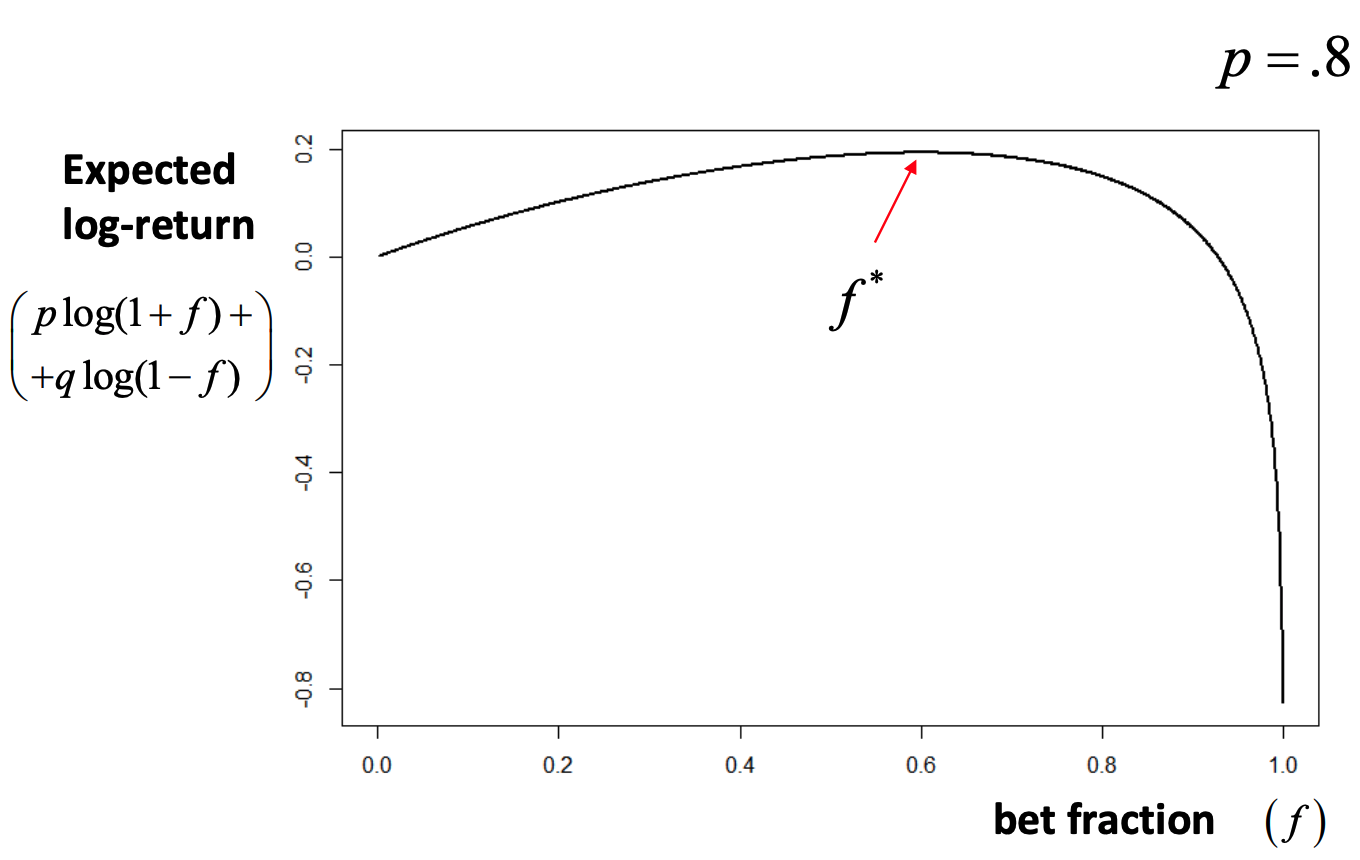
\includegraphics{Notes/Obsidian-Attachments/8-Betting-Strategies.png}

\hypertarget{geometric-average}{%
\subsection{Geometric average}\label{geometric-average}}

Assuming a fixed fraction \(f\) of wealth is bet at each time step. What is the geometric avg of the returns as \(n\to \infty\)?

\[
\begin{aligned}
\text{Let growth rate } r_{i} &\text{ be }:\\
\text{For } i-1 \to i: r_{i} &= \frac{V_{i}}{V_{i-1}}\\
\text{Geometric Average: }&: (r_{1} \times r_{2}\dots \times r_{n})^{1/n} = \left[ \prod^{n}_{i=1}(1+f)^{I_{i}}(1-f)^{1-I_{i}} \right] ^{1/n}\\
&= (1+f)^{\underbrace{ \sum^{n}_{i=1}I_{i}/n }_{ W_{n} }} \times (1-f)^{1/n \sum^{n}_{i=1}(1-I_{i})}\\
&= (1+f)^{W_{n}/n}\times (1-f)^{1-W_{n}/n} \quad \text{where } W_{n}\sim Binom(n,p)
\end{aligned}
\]

So as \(n\to \infty\), \(\frac{W_{n}}{n}\to p\) from LLN, which implies the geometric average converges to:
\[
(1+f)^{p}(1-f)^{1-p}
\]
from the continuous mapping theorem. This is also the expression where if you take the log, you get \(\underbrace{ \log(1+f)np+\log(1-f)nq }_{ G(f) }\) from the {[}{[}\#Finding the Optimal Value{]}{]} section.

\hypertarget{simple-example}{%
\subsection{Simple example}\label{simple-example}}

Consider general sequence of bets, where

\begin{itemize}
\tightlist
\item
  \(1 bet \implies +\$a\) if win and \(−\$b\) if lose
\item
  For previous examples \(a = b = 1\)
\item
  \(P(win)=p\) and \(P(lose)=q\)
\item
  Bet is favorable, i.e.~\(p\cdot a> q\cdot b\)
\item
  Kelly criterion optimal fraction to bet is
  \[
  f^{*} = \frac{pa-qb}{ab}
  \]
\end{itemize}

So
\[
\begin{aligned}
\text{Given }& a = 1, b = 1\\ \\
f^{*} = &\frac{1p-1q}{1\cdot1} = p-q = .55-.45 = .10
\end{aligned}
\]

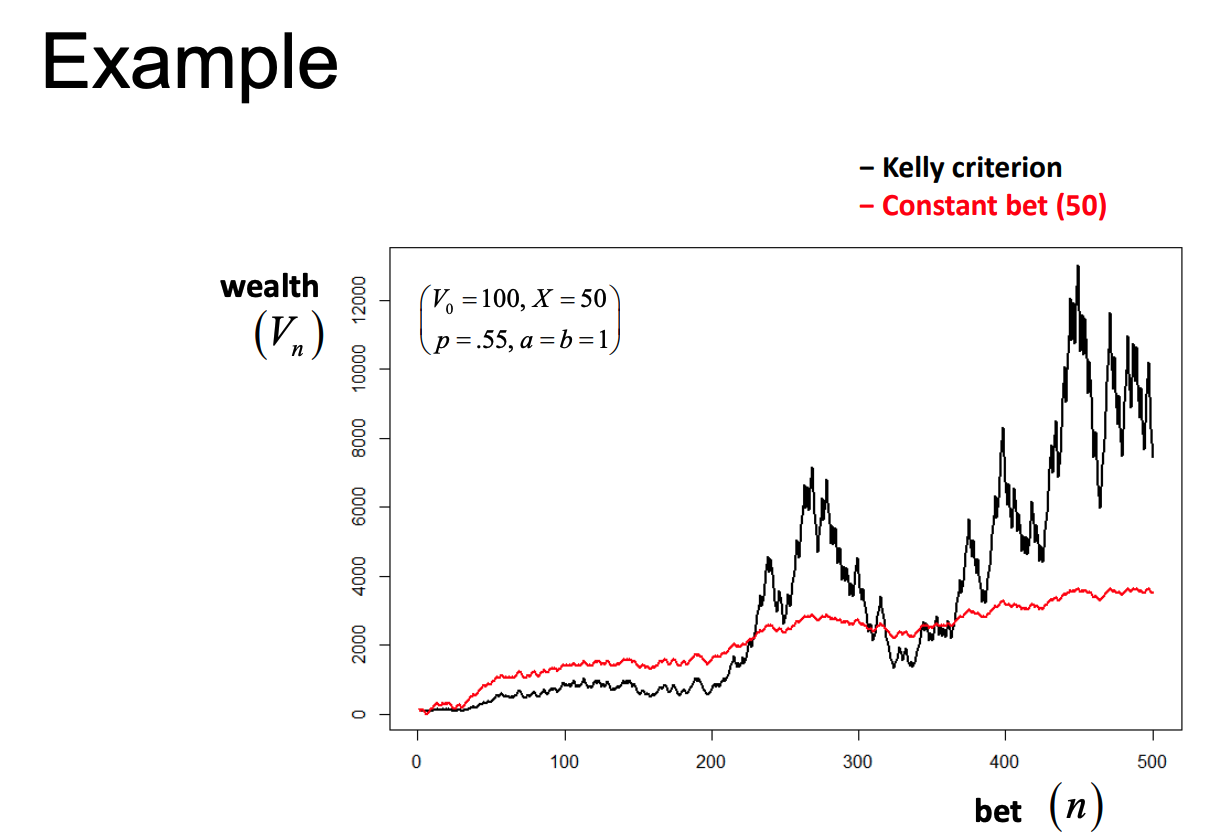
\includegraphics{Notes/Obsidian-Attachments/8-Betting-Strategies-1.png}

\hypertarget{kelly-criterion-in-investing}{%
\subsection{Kelly Criterion in Investing}\label{kelly-criterion-in-investing}}

Consider a situation where you have:
- risk free asset with return \(r_{i}\)
- One risky asset with return \(R_{i}\), with \(\mathbb{E}(R) = \mu, \mathbb{V}(R) = \sigma^{2}\)

Assume we invest fraction \(f\) in the risky asset, and \(1-f\) in the risk free asset.

We first need to show that:
\[
\mathbb{E}\left[ \log\left( \frac{V_{n}}{V_{0}} \right) \right] \approx \log(1+r_{f}) +f\left( \frac{\mu-r_{f}}{1+r_{f}} \right)-f^{2}\left( \frac{\sigma^{2}+(\mu-r_{f})^{2}}{2(1+r_{f})^{2}} \right)
\]

\[
\begin{aligned}
\text{Know: }V_{1} &= V_{0}\cdot f\cdot(1+R) + V_{0}(1-f)(1+r_{f})\\
&= V_{0}[1+fR+(1-f)r_{f}]\\
&= V_{0}[1+r_{f}+f\underbrace{ (R-r_{f}) }_{ \text{Excess ret} }]\\
\implies \frac{V_{1}}{V_{0}} &= \log(1+r_{f}+f(R-r_{f}))\\
\\
\implies \log \left( \frac{V_{n}}{V_{0}} \right) &=  \log \left( \prod^{n}_{t=1} \frac{V_{t}}{V_{t-1}} \right) \\
&= \sum^{n}_{t=1} \log(1+r_{f}+f(R_{t}-r_{f}))\\
\\
\implies \mathbb{E}\left[ \log\left( \frac{V_{n}}{V_{0}} \right) \right] &= \sum^{n}_{t=1}\mathbb{E}[\log(1+r_{f}+f(R_{t}-r_{f}))]\\
& \text{Assuming i.i.d. returns}\\
&= n \mathbb{E}[\log(1+r_{f}+f(R-r_{f}))]
\end{aligned}
\]

We can simplify this using a taylor approx of the function \(\log(1+r_{f}+f(R-r_{f}))\) around \(1+r_{f}\):
\[
\begin{aligned}
\underbrace{ \log }_{ g } \left( \underbrace{ 1+r_{f} }_{ x_{0} }+\underbrace{ f(R_{t}-r_{f} }_{ \delta }) \right) &\approx \underbrace{ \log(1+r_{f}) }_{ g(x_{0}) } + \underbrace{ \frac{1}{1+r_{f}}f(R_{t}-r_{f}) }_{ g'(x_{0}) }+\underbrace{ \frac{1}{2}\left( \frac{f^{2}}{(1+r_{f})^{2}}\right)\delta^{2} }_{ g''(x_{0}) }
\end{aligned}
\]
\[
\begin{aligned}
\mathbb{E}[g(x_{0}-\delta)] \approx \log(1+r_{f}) &+ \frac{1}{1+r_{f}}f\underbrace{ \mathbb{E}(R_{t}-r_{f}) }_{ \mu-r_{f} }+\frac{1}{2}\left( \frac{f^{2}}{(1+r_{f})^{2}}\right)\mathbb{E}[(R_{t}-r_{f})^{2}]\\
\text{Where } \mathbb{E}[(R_{t}-r_{f})^{2}] &= (\sigma^{2}+\mu^{2}+r_{f}^{2}-2\mu r_{f})
\end{aligned}
\]

We can now show that \(f^{*} \approx (1+r_{f}) \frac{(\mu-r_{f})}{\sigma^{2}}\)

\[
\begin{aligned}
\text{Let } G(f) &= \log(1+r_{f})+\frac{f}{1+r_{f}}(\mu-r_{f})-\frac{f^{2}}{2(1+r_{f})^{2}}(\sigma^{2}+\mu^{2}+r_{f}^{2}-2\mu r_{f})
\end{aligned}
\]

\[
\mathbf{\implies f^{*} \approx (1+r_{f}) \frac{\mu-r_{f}}{\sigma^{2}}}
\]

\hypertarget{example-in-investing}{%
\subsubsection{Example in investing}\label{example-in-investing}}

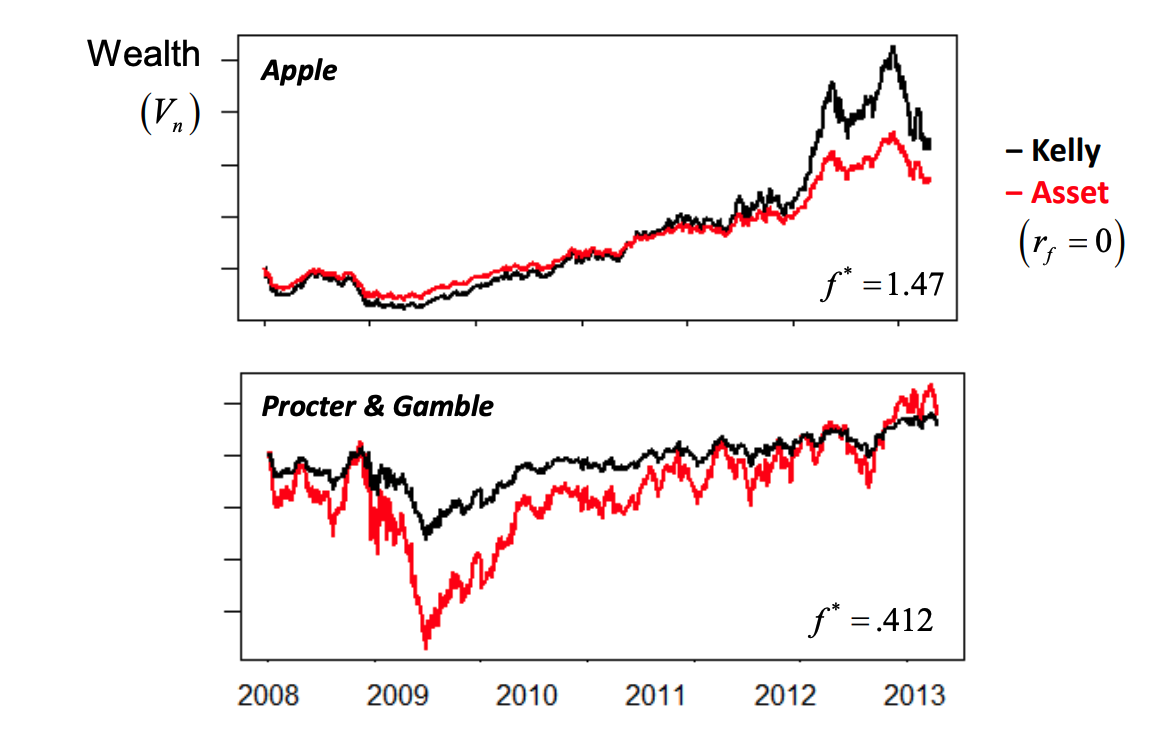
\includegraphics{Notes/Obsidian-Attachments/8-Betting-Strategies-2.png}

\hypertarget{theoretical-properties}{%
\subsection{Theoretical properties}\label{theoretical-properties}}

In the long term \(n\to \infty\), with probability 1, a strategy based on a Kelly criterion will:
- Maximize the limiting exponential growth rate of wealth
- Maximizes median of final wealth
- Half of distribution is above median \& half below it
- Minimizes the expected time required to reach a specified goal for the wealth

\hypertarget{criticisms}{%
\subsection{Criticisms}\label{criticisms}}

It tends to be risky

It works well if you have clear information (what exactly your edge is) and that you have an infinite sequence of gambles

In practice, people will take half of the kelly criterion, as a precaution against high volatility

Most people retire at some point and therefore do not have infinite gambles

\hypertarget{statistical-arbitrage}{%
\chapter{Statistical Arbitrage}\label{statistical-arbitrage}}

Mathematical definition of a ``free lunch''. In the real world, there is never 0 risk. Statistical arbitrage uses ``statistical mispricing'' of assets to make money. This involves long and short positions simultaneously and are typically short-term and market-neutral.

Examples:

\begin{itemize}
\tightlist
\item
  Pairs Trading
\item
  Index Arbitrage
\item
  Volatility Arbitrage
\item
  Algorithmic and High Frequency Trading
\end{itemize}

\hypertarget{pairs-trading}{%
\section{Pairs Trading}\label{pairs-trading}}

Developed in the 80's by Morgan Stanley quants, who made \textasciitilde50 Million in profits in 1987.

\textbf{The idea:} Find pairs of stocks that tend to move together, and once they diverge, you expect them to come back together. If they cross some threshold of divergence, buy the low priced one and sell the higher priced one until they converge.

\textbf{Problem:} If the prices don't converge.

Example of two pairs:

\includegraphics{Notes/Obsidian-Attachments/9-Statistical-Arbitrage.png}

We use log asset prices because it's easier to model with Brownian motion.

\includegraphics{Notes/Obsidian-Attachments/9-Statistical-Arbitrage-1.png}

Using this chart, we can decide the threshold at which to trade the two stocks:

\includegraphics{Notes/Obsidian-Attachments/9-Statistical-Arbitrage-2.png}

\begin{itemize}
\tightlist
\item
  Key: Buy and sell the \textbf{same dollar amount}.
\item
  Buy \(\frac{1}{P2_{0}}\) where \(P2_{o}\) is the opening price of stock 2
\end{itemize}

\includegraphics{Notes/Obsidian-Attachments/9-Statistical-Arbitrage-3.png}

Per \$1 invested, the profit will be:

\[
\frac{1}{P2_{o}}\times P2_{c}-\frac{1}{P1_{o}}\times P1_{c} = \frac{28.07}{27.15}-\frac{30.23}{32.91} = .11532
\]

The profitability is determined by the behaviour of the log asset-price ratio.

\[
\begin{gathered}
\text{Profitable if: } \frac{P1_{c}}{P1_{o}} - \frac{P2_{c}}{P2_{o}} \ne 0\\
\implies \frac{P1_{c}}{P1_{o}} < \text{ or }> \frac{P2_{c}}{P2_{o}}
\end{gathered}
\]

which is equivalent to asking

\[
\begin{aligned}
\frac{P2_{o}}{P1_{o}} &< \text{or} > \frac{P2_{c}}{P1_{c}}\\
&\iff\\
\log(\frac{P2_{o}}{P1_{o}}) &< \text{or} > \log(\frac{P2_{c}}{P1_{c}})
\end{aligned}
\]
\textgreater Profitability is determined by log-ratio of prices. We say \(< \text{ or } >\) just because we only care that there exists a difference, but not which one exactly is the larger of the two.

\includegraphics{Notes/Obsidian-Attachments/9-Statistical-Arbitrage-5.png}

We can also show market-neutrality:
\[
\begin{aligned}
CAPM &\implies \begin{cases}
R1 = \beta\cdot R_{M} + \epsilon_{1} \\
R2 = \beta\cdot R_{M} + \epsilon_{2} \\
\end{cases} \implies
\begin{cases}
\frac{P1_{c}}{P1_{o}} = 1+R1 = 1+\beta\cdot R_{M} + \epsilon_{1} \\
\frac{P2_{c}}{P2_{o}} = 1+R2 = 1+\beta\cdot R_{M} + \epsilon_{2} \\
\end{cases}\\
&\implies \frac{P1_{c}}{P1_{o}} - \frac{P2_{c}}{P1_{o}} = \frac{P2_{c}}{P2_{o}} = (1+\beta\cdot R_{M} + \epsilon_{1}) - (1+\beta\cdot R_{M} + \epsilon_{2}) = \epsilon_{1}-\epsilon_{2}\\
\end{aligned}
\]

Where \(\epsilon_{1}-\epsilon_{2}\) is independent of market return \(R_{M}\).

\hypertarget{what-could-go-wrong}{%
\subsection{What could go wrong}\label{what-could-go-wrong}}

When the prices don't converge, and the log ratio of prices don't go back to the mean. (Mean-reverting)

\includegraphics{Notes/Obsidian-Attachments/9-Statistical-Arbitrage-4.png}

\hypertarget{other-things-to-consider}{%
\subsection{Other things to consider}\label{other-things-to-consider}}

\begin{enumerate}
\def\labelenumi{\arabic{enumi}.}
\tightlist
\item
  Determine which pairs to trade
\item
  When to open a position (the threshold)
\item
  What amounts to buy/sell
\item
  When to close trade
\item
  When to bail out of trade
\end{enumerate}

Need to create a statistical/mathematical model to help make decisions on these items to consider.

\hypertarget{determining-which-pairs-to-trade}{%
\subsubsection{1. Determining which pairs to trade}\label{determining-which-pairs-to-trade}}

For a market with \(N\) assets, there are max \(_{n}C_{2}\) pairs that could be made which is in the order of \(n^{2}\).

We only want pairs who's log-ratio has \textbf{strong mean reversion}. This is not the same as simply having a constant mean. It depends on the dynamics of log-ratio process. For example, ARMA models have mean reversion properties but random walk processes/brownian motion do not have the mean reversion property.

\hypertarget{example-1-log}{%
\subsubsection{Example 1: Log}\label{example-1-log}}

Let \(X_{t} = \log(\frac{P1_{t}}{P2_{t}}) \sim^{iid} N(0,\sigma^{2}), \ \forall t=1,2,\dots\)

If \(X_{0} = 2\sigma\), what's the expected time until \(X_{T}\leq 0\)?

On any day \(t\), \(\mathbb{P}(X_{t}\leq 0) = 0.5\) by symmetry

\[
\begin{aligned}
\text{Let } T &= \# \text{ days until } X_{t} \leq 0 \text{ for the first time}\\
&= \text{(hitting time)}\\
&= \# \text{ trials until 1st success } x_{t} \leq 0\\
\implies T &\sim \text{Geometric}\left( p=\frac{1}{2} \right)\\
PMF \ \ p_{T}(t) &= \left( \frac{1}{2} \right)^{t} \quad \forall t \geq 1\\
\mathbb{E}(T) &= \frac{1}{p} = 2
\end{aligned}
\]

\hypertarget{example-2-bm}{%
\subsubsection{Example 2: BM}\label{example-2-bm}}

Let \(X_{t} = \log(\frac{P1_{t}}{P2_{t}}) \sim\) Brownian Motion (BM) (continuous time Random Walk)
For any \(X_{0}=c > 0\), show that the expected time until \(X_{T}\leq 0\) is infinite.

\[
\begin{aligned}
\text{Let } T_{c} &= \{\text{first time std BM w/} W_{0} =0 \text{ hits level c}\}\\
\text{Let }M_{t} &= \max\left\{ W_{u} ; 0 \leq u \leq t \right\}
\implies M_{t} \sim |W_{t}|
\end{aligned}
\]

\includegraphics{Notes/Obsidian-Attachments/9-Statistical-Arbitrage-14.png}

Which tells you that the distribution of the \(M_{t}\) follows the same distribution of the absolute value of the Brownian Motion.

This means:
\[
\begin{aligned}
\mathbb{P}(T_{c}\leq t) = \mathbb{P}(M_{t}\geq c) = \mathbb{P}(|\underbrace{ W_{t} }_{ \sim N_(0,t) }| \geq c) = 2 \cdot \Phi\left( -\frac{c}{\sqrt{ t }} \right)
\end{aligned}
\]

\emph{Where \(\Phi\) is the CDF of the std normal.}

As we look at the two tails of the normal after standardizing, but we take the area under the lower tail (-c).

\[
\begin{aligned}
\implies \text{PDF of }& T_{c} \text{ is given by } f(t)\\
f(t) &= \frac{\delta}{\delta t} \underbrace{ \mathbb{P}(T_{c}\leq t) }_{ F(t) } = \frac{\delta}{\delta t}\left[ 2\cdot \Phi\left( -\frac{c}{\sqrt{ t }} \right) \right]\\
&= 2 \frac{\phi\left( -\frac{c}{\sqrt{ t }} \right)\delta}{\delta t}\left( -\frac{c}{\sqrt{ t }} \right)\\
&= 2\phi\left( -\frac{c}{\sqrt{ t }} \right)\cdot\left( -\left( -\frac{1}{2} \frac{c}{\sqrt{ t^{3} }}\right) \right)\\
&= \frac{1}{\sqrt{ 2 \pi }}e^{-1/2 \cdot c^{2}/t}\cdot \frac{c}{\sqrt{ t^{3} }}
\end{aligned}
\]

So the expected value of hitting time is:
\[
\begin{aligned}
\mathbb{E}(T_{c}) &= \int ^{\infty}_{0} t\cdot f(t) \, dt\\ 
&= \int ^{\infty}_{0}t \frac{c}{\sqrt{ 2\pi t^{3} }}e^{-1/2 \cdot c^{2}/2} \, dt\\
&= \frac{c}{\sqrt{ 2\pi }} \int^{\infty}_{0} \frac{1}{\sqrt{ t }}e^{-c^{2}/2t} \, dt\\
&\geq \frac{c'}{\sqrt{ 2\pi }}\int^{\alpha}_{0} \frac{1}{\sqrt{ t }} \, dt + \int ^{\infty}_{\alpha} \frac{1}{\sqrt{ t }}e^{-c^{2}/2t} \, dt \to \infty\\
\\
\implies \mathbb{E}[T_{c}] &= \infty
\end{aligned}
\]

A stationary process ensures mean reversion. Thats why we use stationary processes to model the log-ratio.

\hypertarget{mean-reversion}{%
\subsection{Mean Reversion}\label{mean-reversion}}

Mean reversion suggests log-ratio process are stationary.

Stationary processes are guaranteed to converge back to their mean within a reasonable time.

\begin{itemize}
\tightlist
\item
  Marginal distribution has constant mean, variance, and covariance between two stationary variables only depends on the distance between times
\item
  Auto-Correlation Function (ACF) \(\rho(h), \forall h=0,1, \ldots\) describes (linear) dependence at lag \(h=|t-s|\)
\end{itemize}

\[
\begin{aligned}
\mathbb{E}[X_{t}] &= \mu  \quad \forall t\\
\mathbb{V}[X_{t}] &= \sigma < \infty \quad \forall t\\
Cov(X_{t},X_{s}) &= Cov(X_{t+r},X_{s+r}) \quad \forall r,s,t
\end{aligned}
\]

\includegraphics{Notes/Obsidian-Attachments/9-Statistical-Arbitrage-6.png}

\hypertarget{integrated-series}{%
\subsection{Integrated Series}\label{integrated-series}}

In general, asset log-prices which are random walks, are not stationary. They are unpredictable. However, the \textbf{log returns} \(r_{t} = \log(\frac{S_{t}}{S_{t-1}})\) follow a stationary process, whereas the asset log-prices \(\log(S_{t}) = \log(S_{0}) + \sum^{t}_{i=1}r_i\) are random walks.

\begin{quote}
A variable that is not stationary but it's differences are, is called an integrated series. \(\left\{ X_{t} \right\}\) is not stationary but \(\left\{ \nabla X_{t} = X_{t} - X_{t-1}\right\}\) is.
\end{quote}

\includegraphics{Notes/Obsidian-Attachments/9-Statistical-Arbitrage-7.png}

\hypertarget{cointegration}{%
\subsection{Cointegration}\label{cointegration}}

Consider two integrated series \(\left\{ X_{t}, Y_{t} \right\}\) which behave as random walks, but if they seem to have some constant (stationary) relationship when linearly combined then they are called cointegrated.
\[
\exists \ \alpha\ s.t.\ X_{t} + \alpha Y_{t} \sim Stationary
\]

\hypertarget{ex-yield-rate}{%
\subsubsection{Ex: Yield Rate}\label{ex-yield-rate}}

\includegraphics{Notes/Obsidian-Attachments/9-Statistical-Arbitrage-8.png}

\begin{quote}
The short, medium, and long term rates are considered cointegrated as they individually follow a random walk, but they do it together.
\end{quote}

\hypertarget{ex-math}{%
\subsubsection{Ex: Math}\label{ex-math}}

Let \(\left\{ W_{t} \right\}\) be a random walk, and
\[
\begin{cases}
X_{t} = W_{t} + \epsilon_{t} \\
Y_{t} = W_{t} + \nu_{t}
\end{cases}
\]

where \(\epsilon, \nu \sim^{iid} N(0,\sigma^{2})\)

We can show \(\left\{ X_{t},Y_{t} \right\}\) are cointegrated. (They are not stationary, but their 1st order different is stationary)

\[
\mathbb{V}(X_{t}) = \mathbb{V}[W_{t}+\epsilon_{t}] = \overbrace{ \mathbb{V}(W_{t}) }^{ t \sigma_{w}^{2} } + \overbrace{ \mathbb{V}(\epsilon_{t}) }^{ \sigma^{2} } = t\sigma_{w}^{2}+\sigma^{2} \implies \text{not stationary}
\]
Which is the same case for \(Y_{t}\). Looking at the first order differences:

\[
\begin{gathered}
\nabla X_{t} = X_{t}-X_{t-1} = W_{t}+\epsilon_{t} -W_{t-1}+\epsilon_{t-1} = (W_{t}-W_{t-1})+\epsilon_{t}+\epsilon_{t-1}\\
\implies \mathbb{V}(\nabla X_{t}) = \sigma^{2} \text{stationary}
\end{gathered}
\]

To show cointegration, we much show \(X_{t}-Y_{t}\) is stationary.

\[
\begin{gathered}
X_{t}-Y_{t} = (W_{t}+\epsilon_{t})-(W_{t}+\nu_{t}) = \epsilon_{t} + \nu_{t} \text{sum of iid sequences}\\
\implies \begin{cases}
\mathbb{E}(X_{t}-Y_{t}) = 0 \\
\mathbb{V}(X_{t}-Y_{t}) = 2\sigma^{2} \\
Cov(X_{t}-Y_{t}, X_{t+h}-Y_{t+h}) = \rho |h| ??
\end{cases}
\end{gathered}
\]

For pairs trading, we want assets which are cointegrated (their log difference is stationary)

\hypertarget{stationarity}{%
\subsection{Stationarity}\label{stationarity}}

\includegraphics{Notes/Obsidian-Attachments/9-Statistical-Arbitrage-9.png}

\begin{quote}
Time series is not always a good indicator of a random walk. We can use a ACF to determine it. Linear decline -\textgreater{} random walk
\end{quote}

\hypertarget{tests}{%
\subsubsection{Tests}\label{tests}}

There also exists stationarity tests:

Hypothesis test for \(\left\{\begin{array}{l}H_0 \text { : series is integrated } \\ H_1 \text { : series is stationary }\end{array}\right.\)
- Idea: fit \(X_t=\beta X_{t-1}+\varepsilon_t\) to data and test \(\left\{\begin{array}{l}H_0: \beta=1 \\ H_1: \beta<1\end{array}\right.\) E.g. For \(n=1000\)
\textbar{} Model \textbar{} Test statistic \textbar{} P-value \textbar{}
\textbar----------------------------------\textbar----------------\textbar---------------------------------\textbar{}
\textbar{} \(X_t=X_{t-1}+\varepsilon_t\) \textbar{} -1.9027 \textbar{} 0.6195 \textbar{}
\textbar{} \(X_t=+.95 X_{t-1}+\varepsilon_t\) \textbar{} -5.6161 \textbar{} \(<<.01\) \textbar{}
\textbar{} \(X_t=-.95 X_{t-1}+\varepsilon_t\) \textbar{} -232.4851 \textbar{} \(<.01\) \textbar{}

But if we're trying to check if a linear combination of assets is stationary, its difficult because we don't know the linear combination to look for. There are two tests for cointegration:

\begin{itemize}
\tightlist
\item
  \textbf{Engle-Granger two-step method}: Run linear regression and look for potential cointegrated relationship, finding the combination that minimizes squared errors. Then the errors are tested for stationarity (converge to 0)
\item
  \textbf{Vector Error Correction models (VECM)}: Covered in time series, a part of VAR models
\end{itemize}

\hypertarget{two-step-method-example}{%
\subsubsection{Two step method example}\label{two-step-method-example}}

First we fit a linear regression to obtain the slope (not useful), and the intercept (need to subtract from errors).

\includegraphics{Notes/Obsidian-Attachments/9-Statistical-Arbitrage-10.png}

\begin{quote}
Now we can look at the errors (minus the intercept so its 0 centered) and run stationarity tests on them. We would trade stocks with the highest metrics, although this method is not optimal since our results could be arbitrary.
\end{quote}

\begin{quote}
If we did the regression swapping the variables, the p-value could differ a lot
\end{quote}

\includegraphics{Notes/Obsidian-Attachments/9-Statistical-Arbitrage-11.png}

\hypertarget{spurious-regression}{%
\subsection{Spurious regression}\label{spurious-regression}}

Two totally independent stocks may show some false linear relationship.

Consider 2 independent random walks \(\left\{W_t, V_t\right\}\)
- When you regress \(W_t=\beta_0+\beta V_t+e_t, t=1, \ldots, n\) you are NOT guaranteed that \(\hat{\beta} \rightarrow 0\) as the sample size \(n \rightarrow \infty\) (i.e.~not consistent)!!!
Effect called spurious (fake) regression
- Results of random walk (integrated series) regressions are NOT reliable
- To address this problem \& estimation errors, use Phillips-Ouliaris stationarity test in 2 step method

\begin{quote}
Bottom line is using VAR models is superior than the two step test/using linear regression. A multivariate time series model is best.
\end{quote}

\hypertarget{financial-indices}{%
\section{Financial Indices}\label{financial-indices}}

Indices measure value/performance of financial markets. E.g.,
- Dow-Jones Industrial Average (DJIA): Simple average of 30 major US stock prices (since 1896)
- Standard \& Poor (S\&P) 500: Weighted (cap-base) average of 500 large NYSE \& NASDAQ listed companies
Financial indices are NOT traded instruments
However, there are many financial products whose value is directly related to indices:
- Mutual funds: e.g., Vanguard 500 Index Fund
- Exchange-Traded-Funds (ETF's): e.g., SPDR or iShares S\&P500 Index
- Futures: e.g., E-Mini S\&P futures

\hypertarget{index-arbitrage}{%
\section{Index Arbitrage}\label{index-arbitrage}}

\begin{itemize}
\tightlist
\item
  Financial products based on indices essentially offer a sophisticated version of multivariate cointegration
\item
  Index of \#N assets \(\left\{S_i\right\}_{i=1}^N\) w/ weights \(\left\{w_i\right\}_{i=1}^N\) \(\Rightarrow\) Index level: \(I(t)=\sum_{i=1}^N w_i \times S_i(t)\)
\item
  Instrument tracking index \(F(t)\) (e.g.~futures)
\item
  Known cointegration relationship:
  \[
  F(t)-I(t)=F(t)-\sum_{i=1}^N w_i \times S_i(t) \sim \text { stationary }
  \]
\end{itemize}

\includegraphics{Notes/Obsidian-Attachments/9-Statistical-Arbitrage-12.png}

\hypertarget{volatility-arbitrage}{%
\section{Volatility Arbitrage}\label{volatility-arbitrage}}

\begin{itemize}
\tightlist
\item
  VolArb is implemented with derivatives, primarily options
\end{itemize}

To fix ideas, consider European options:
- For Black-Scholes formula, only unobserved input is volatility \(\sigma\), which has to be estimated
- How does volatility affect Call/Put prices?
- Implied volatility \(\sigma_i\) is input which makes Black-Scholes price equal to observed market price
- \(\sigma_i\) is not estimated from underlying asset dynamics
- Imagine you know volatility will increase in the future, beyond what current options prices warrant (implied vol σi ).
- How can you take advantage of this?
- Eliminate effects of asset movement by delta-neutral strategy
- Profit by large moves, irrespective of direction

\begin{itemize}
\tightlist
\item
  VolArb relies on predicting (implied) volatility of underlying asset
\item
  Common approach is to describe the evolution of volatility with GARCH (Generalized AutoRegressive Conditional Heteroskedasticity) models
  \[
  \begin{gathered}
  y_t=\sigma_t \cdot \varepsilon_t, \varepsilon_t \sim^{i i d} N(0,1) \\
  \sigma_t^2=\alpha_0+\sum_{j=1}^p \alpha_j y_{t-j}^2+\sum_{k=1}^q \beta_k \sigma_{t-k}^2
  \end{gathered}
  \]
\item
  Essentially, an autoregressive model for conditional variance
\end{itemize}

\hypertarget{e.g.-delta-hedged-long-call}{%
\subsection{E.g. Delta-hedged long call}\label{e.g.-delta-hedged-long-call}}

\includegraphics{Notes/Obsidian-Attachments/9-Statistical-Arbitrage-13.png}

\hypertarget{high-frequency-trading}{%
\section{High Frequency Trading}\label{high-frequency-trading}}

\begin{itemize}
\tightlist
\item
  HFT uses algorithmic trading over very short holding periods, profiting from very small price discrepancies by trading frequently and at large volumes
\item
  HFT employs predictive algorithms for machine learning and data mining

  \begin{itemize}
  \tightlist
  \item
    Essentially, tries to discover patterns of trading activity \& profit by preempting them
  \item
    This includes traditional method like index arbitrage, but also others which might not have any intuitive interpretation
  \end{itemize}
\end{itemize}

\hypertarget{monte-carlo-simulation}{%
\chapter{Monte-Carlo Simulation}\label{monte-carlo-simulation}}

Primarily dealing with option pricing. There are three basic numerical option pricing methods:

\begin{itemize}
\tightlist
\item
  Binomial Trees (BT)

  \begin{itemize}
  \tightlist
  \item
    Don't need sophisticated mathematical or stochastic analysis, just backward induction
  \item
    Useful in many cases
  \end{itemize}
\item
  Finite Difference (FD)

  \begin{itemize}
  \tightlist
  \item
    Uses the Black-Scholes PDE
  \item
    Not discussed much in the stats program
  \end{itemize}
\item
  Monte-Carlo Simulation

  \begin{itemize}
  \tightlist
  \item
    Based on the stochastic differential equation (determines evolution of asset-price)
  \item
    Easy to program and risk-neutral
  \item
    Really shines with multiple dimensions (many factors, path/multi-asset)
  \end{itemize}
\end{itemize}

\includegraphics{Notes/Obsidian-Attachments/10-Monte-Carlo.png}

\hypertarget{brownian-motion}{%
\section{Brownian Motion}\label{brownian-motion}}

Any martingale can be represented as an integral of brownian motion.

Brownian Motion (BM) forms the building block of continuous stochastic models
Standard BM \(\left\{W_t\right\}\) is such that

\[
W_0=0 \quad \& \quad (W_t-W_s) \mid W_s \sim N(0, t-s)
\]
Arithmetic BM (ABM) \(\left\{X_t\right\}\) with drift \(\mu\) \& volatility \(\sigma\) is

\[
X_0=0 \quad \& \quad \left(X_t-X_s\right) \mid X_s \sim N\left(\mu(t-s), \sigma^2(t-s)\right)
\]

\begin{itemize}
\tightlist
\item
  In form of Stochastic Differential Equation (SDE)
\end{itemize}

\[
d X_t=\mu d t+\sigma d W_t \Leftrightarrow X_t-X_0=\mu t+\sigma\left(W_t-W_0\right)
\]

\hypertarget{properties-of-the-multivariate-normal}{%
\section{Properties of the Multivariate Normal}\label{properties-of-the-multivariate-normal}}

If
\[
\mathbf{X}=\left[
\begin{array}{c}
\mathbf{X}_1 \\
\mathbf{X}_2 \\
\end{array}
\right] 
\sim \mathbf{N}\left(\boldsymbol{\mu}=\left[
\begin{array}{c} 
\boldsymbol{\mu}_1 \\
\boldsymbol{\mu}_2
\end{array}
\right],
\boldsymbol{\Sigma}=\left[
\begin{array}{cc}
\boldsymbol{\Sigma}_{11} & \boldsymbol{\Sigma}_{12} \\ 
\boldsymbol{\Sigma}_{21} & \boldsymbol{\Sigma}_{22} 
\end{array}\right]
\right)
\]
\includegraphics{Notes/Obsidian-Attachments/10-Simulation-3.png}, then:

\begin{longtable}[]{@{}
  >{\raggedright\arraybackslash}p{(\columnwidth - 2\tabcolsep) * \real{0.0627}}
  >{\raggedright\arraybackslash}p{(\columnwidth - 2\tabcolsep) * \real{0.9373}}@{}}
\toprule\noalign{}
\begin{minipage}[b]{\linewidth}\raggedright
Property
\end{minipage} & \begin{minipage}[b]{\linewidth}\raggedright
Formula
\end{minipage} \\
\midrule\noalign{}
\endhead
\bottomrule\noalign{}
\endlastfoot
Marginals: & \(\quad \mathbf{X}_1 \sim \mathbf{N}\left(\boldsymbol{\mu}_1, \boldsymbol{\Sigma}_{11}\right)\) \\
Linear combinations: & \(\mathbf{a}+\mathbf{B}^{\top} \mathbf{X} \sim N\left(\mathbf{a}+\mathbf{B}^{\top} \boldsymbol{\mu}, \mathbf{B}^{\top} \boldsymbol{\Sigma} \mathbf{B}\right)\) \\
Conditionals : & \(\mathbf{X}_1 \mid\left(\mathbf{X}_2=\mathbf{x}\right)\sim\mathrm{N}\left(\boldsymbol{\mu}_1+\boldsymbol{\Sigma}_{12}\boldsymbol{\Sigma}_{22}^{-1}\left(\mathbf{x}\boldsymbol{\mu}_2\right),\boldsymbol{\Sigma}_{11}-\boldsymbol{\Sigma}_{12}\boldsymbol{\Sigma}_{22}^{-1}\boldsymbol{\Sigma}_{21}\right)\) \\
\end{longtable}

If \(\Sigma_{12}=0\) then \(\mathbf{X_{1}}|\mathbf{X_{2}}=x \sim N(\mu_{1},\Sigma_{11})\)

Using these properties, we can do calculations for brownian motion

\hypertarget{ex-distribution-given-x_s}{%
\subsection{Ex: Distribution given X\_s}\label{ex-distribution-given-x_s}}

Finding the distribution of \(X_{t}|X_{s} = x, t>s\) for \(dX_{t} = \mu dt+\sigma dW\)
\[
\begin{aligned}
\left[ \begin{array}{c}
X_{s} \\
X_{t}
\end{array} \right] \sim N(
\left[ \begin{array}{c}
\mu_{s} \\
\mu_{t}
\end{array} \right],
\left[ \begin{array}{cc}
\sigma^{2}s & \sigma s \\
\sigma s & \sigma^{2}t
\end{array} \right] )
\end{aligned} \iff \left[ \begin{array}{c}
X_{t}  \\
X_{s}
\end{array}  \right] \sim N(\mu \left[ \begin{array}{c}
t \\
\hline s
\end{array} \right],
\sigma^{2} \left[ \begin{array}{cc}
t & s \\
s & s
\end{array} \right] )
\]
\includegraphics{Notes/Obsidian-Attachments/10-Simulation-4.png}
Because
\[
\begin{aligned}
Cov(W_{s},W_{t}) &= Cov(W_{s}, W_{s}+(W_{t}-W_{s}))\\
&= Cov(W_{s}, W_{s}) + \underbrace{ Cov(W_{s}, (W_{t}-W_{s})) }_{ =0 }\\
&= Var(W_{s}) = s
\end{aligned}
\]

Which gives:
\[
\begin{aligned}
X_{t} | X_{s} = x &\sim N\left( \mu t + \sigma^{2}s \frac{1}{\sigma^{2}s} (x-\mu s), \sigma^{2}\left( t-s \frac{1}{8}8 \right) \right)\\
&\sim N(x + \mu (t-s), \sigma^{2}(t-s))
\end{aligned}
\]

\hypertarget{ex-brownian-bridge-distribution-given-x_t}{%
\subsection{Ex: Brownian Bridge (Distribution given X\_t)}\label{ex-brownian-bridge-distribution-given-x_t}}

Find the distribution of \(X_{s} | X_{t} = x, s\in (0,t)\) for \(dX_{t} = \mu dt + \sigma dW_{t}\)

\[
\begin{aligned}
\left[ \begin{array}{c}
X_{s} \\
X_{t}
\end{array} \right] &\sim N(\mu \left[ \begin{array}{c}
s \\
t
\end{array} \right], \sigma^{2} \left[ \begin{array}{cc}
s & s \\
s & t
\end{array} \right]  )\\
\end{aligned}
\]
\includegraphics{Notes/Obsidian-Attachments/10-Simulation-5.png}
\[
\begin{aligned}
\implies X_{s} | X_{t} = x &\sim N\left( \underbrace{ \mu s+\frac{s}{t}(x-\mu t) }_{ \mu s+\frac{s}{t}x-\mu s },
\sigma^{2}\left( s-\frac{s}{t}s \right)\right)\\
&\sim N\left( \frac{s}{t}x, \sigma^{2} \frac{s(t-s)}{t}\right)
\end{aligned}
\]

May be useful for generating brownian motion paths where I know that at time \(T\), I have value of \(x\).

\hypertarget{geometric-brownian-motion}{%
\section{Geometric Brownian Motion}\label{geometric-brownian-motion}}

A transformation of the arithmetic brownian motion. We use this to avoid negative values.

Process \(\left\{S_t\right\}\) whose logarithm follows ABM
\[
\begin{aligned}
& \log \left(S_t\right)-\log \left(S_0\right)=\log \left(\frac{S_t}{S_0}\right)=X_t \sim N\left(\mu t, \sigma^2 t\right) \Leftrightarrow \\
& \Leftrightarrow S_t=S_0 \exp \left\{X_t\right\} \sim S_0 \times \log \operatorname{Normal}\left(\mu t, \sigma^2 t\right)
\end{aligned}
\]

\begin{quote}
As the log of \(\exp \left\{ X_{t} \right\} = X_{t}\) and \(X_{t} \sim Normal(\mu t, \sigma^{2}t)\)
\end{quote}

Expressed in terms of SDE:
\[
d X_t=d \log \left(S_t\right)=\mu d t+\sigma d W_t \Leftrightarrow d S_t=\left(\mu+\frac{\sigma^2}{2}\right) S_t d t+\sigma S_t d W_t
\]

\hypertarget{risk-neutral-pricing}{%
\section{Risk-Neutral Pricing}\label{risk-neutral-pricing}}

\begin{itemize}
\tightlist
\item
  Assuming Geometric BM for asset \(\left\{S_t\right\}\) and risk-free interest rate \(r\), there exists a probability measure such that

  \begin{itemize}
  \tightlist
  \item
    \[
    d S_t=r S_t d t+\sigma S_t d W_t \Rightarrow S_t \sim S_0 \times \log N\left(\left(r-\frac{\sigma^2}{2}\right) t, \sigma^2 t\right)\]
  \item
    Under this measure, discounted asset prices are martingales
  \item
    Called risk-neutral (RN) or equivalent martingale measure
  \end{itemize}
\item
  The arbitrage-free price of any European derivative with payoff \(G_T=f\left(S_T\right)\) is given by discounted expectation w.r.t. RN measure
  \[
  G_0=\mathbb{E}\left[e^{-r T} G_T\right]=\mathbb{E}\left[e^{-r T} f\left(S_T\right)\right]
  \]
\end{itemize}

\begin{quote}
We just need to figure out that expected value to obtain the price at time \(0\).
\end{quote}

\hypertarget{ex-rn-pricing}{%
\subsection{Ex: RN Pricing}\label{ex-rn-pricing}}

We'll show that under risk-neutral pricing measure,

\[
\mathbb{E}(S) = S_{0}e^{rt}
\] (a martingale)
then we would have

\[
\mathbb{E}\left( \frac{S_{t}}{e^{rt}}\right) = S_{0} \quad \text{ or more generally } \mathbb{E}\left( \frac{S_{t}}{e^{rt}} |S_{s} \right) = \frac{S_{s}}{e^{rt}}
\]
Proof:
\[
\begin{aligned}
\mathbb{E}(S_{t}) &= \mathbb{E}(S_{0}e^{\log(S_{t}/S_{0})})\\
&= S_{0}\mathbb{E}(e^{Y}) \text{ where } Y=\log\left( \frac{S_{t}}{S_{0}} \right) \sim N\left( \left( r-\frac{\sigma^{2}}{2} \right)t, \sigma^{2}t \right)\\
\end{aligned}
\]

We can use the Normal MGF \(\mathbb{E}(e^{X})\) if \(X\sim N(\mu, \sigma^{2})\):
\[
m_{X}(z) = e^{\mu z+(1/2) \cdot \sigma^{2}z^{2}}
\]

In this case, we have
\[
\begin{aligned}
m_{Y}(1) = \exp \left\{ \overbrace{ \left( r-\frac{\sigma^{2}}{2} \right) }^{ \mathbb{E}(Y) } t + \overbrace{ \frac{1}{2} \sigma^{2}t }^{ \mathbb{V}(Y) }\right\}  = \exp \left\{  rt-\frac{\sigma^{2}}{2} t + \frac{\sigma^{2}}{2} t\right\} = S_{0}e^{rt}
\end{aligned}
\]

\hypertarget{ex-find-price-of-forward-contract-no-dividends}{%
\subsection{Ex: Find price of forward contract (no dividends)}\label{ex-find-price-of-forward-contract-no-dividends}}

\[
G_{T} = f(S_{T}) = (S_{T} - F_{0,T}) \quad \text{ where } F_{0,T} = S_{0}\cdot e^{rT}
\]

We know \(G_{0}=0\) (forward contracts involve no cashflow at \(t=0\))

By the RN pricing: \(G_{0} = \mathbb{E}[e^{-rT}G_{T}]\)

\[
\begin{gathered}
\implies 0 = \mathbb{E}\left[\underbrace{  e^{-rT} }_{ \text{const, can remove} } (S_{T}-F_{0,T}) \right]\\
\implies 0=\mathbb{E}(S_{T}) - F_{0,T}\\
\implies F_{0,T} = \mathbb{E}(S_{T}) = e^{rT}\mathbb{E}(\underbrace{ e^{-rT}S_{T} }_{ S_{0}e^{rT} = S_{T}  \sim mtgl}) = e^{rT}S_{0}
\end{gathered}
\]

\hypertarget{estimating-expectations}{%
\subsection{Estimating Expectations}\label{estimating-expectations}}

If \(\mathbb{E}(e^{-rT}f(S_{t}))\) cannot be calculated exactly, it can be estimated/approximated by simulation.

\begin{itemize}
\tightlist
\item
  Generate \# N independent random variates \(S_{i}(T), i=1,\dots,N\) based on RN measure
\item
  By Strong LLN

  \begin{itemize}
  \tightlist
  \item
    \[
    \hat{G}_{0} = \frac{1}{N} \sum^{N}_{i=1}e^{-rT}f(S_{i}(T)) \to \mathbb{E}(e^{-rT}f(S_{T}))
    \] with probability 1
  \end{itemize}
\item
  By the CLT

  \begin{itemize}
  \tightlist
  \item
    \[
    \frac{\hat{G}_0-G_0}{s_G / \sqrt{n}} \sim^{a p p r} . N(0,1), \text { where } s_G^2=\frac{1}{n-1} \sum_{i=1}^n\left[e^{-r T} f\left(S_i(T)\right)-\hat{G}_0\right]^2
    \]
  \end{itemize}
\end{itemize}

\begin{quote}
If you can express the quantity you're looking for as an expected value, you can run a simulation and it will approximate the value you're looking for
\end{quote}

\begin{quote}
How do you run a simulation experiment to approximate a probability?
\(\mathbb{P}(A)=\mathbb{E}(I_{A})\) the indicator variable of a given event \(A\).
\end{quote}

\hypertarget{ex-show-estimator-is-consistent}{%
\subsection{Ex: Show estimator is consistent}\label{ex-show-estimator-is-consistent}}

Estimator: \(\mathbb{E}[e^{-rT}f(S_{T})]\)

Build a 95\% confidence interval for \(G_{0}\) as well
\[
\begin{aligned}
\mathbb{E}(\hat{G_{0}}) &= \mathbb{E}\left[ \frac{1}{n}\sum^{n}_{i=1} e^{-rT}f(S_{i}(T)) \right]\\
&= \frac{1}{n}\sum^{n}_{i=1}\underbrace{ \mathbb{E}[e^{-rT}f(S_{i}(T))] }_{ G_{1}? } = \frac{1}{n}nG_{0} = G_{0}
\end{aligned}
\]

Confidence interval:
\[
\hat{G_{0}} \pm 1.96 \times \frac{SG}{\sqrt{ n }}
\]

\begin{quote}
Need 4 times the samples to double the accuracy (scaled by \(\sqrt{ n }\))
\end{quote}

\hypertarget{european-call}{%
\section{European Call}\label{european-call}}

Estimating European call price w/ simulation

\begin{itemize}
\tightlist
\item
  Asset price dynamics: \(dS_{t} = rS_{t}dt +\sigma S_{t}dW_{t}\)
\item
  Payoff function for strike \(K\) and maturity \(T\): \(f(S_{t})=(S_{T} - K_{T})\)
\end{itemize}

Generate random asset price variates as:
\[
S_i(T)=S(0) \times \exp \left\{\left(r-\frac{\sigma^2}{2}\right) T+\sigma \sqrt{T} \times Z_i\right\}
\]
where \(Z_i\) is standard Normal variate

Where the x-axis is \(S_t\), and y-axis is the payoff \(G_{t}\)

\begin{Shaded}
\begin{Highlighting}[]
\NormalTok{top=19;bottom={-}1;left={-}1;right=18}
\NormalTok{{-}{-}{-}}
\NormalTok{y=0|x\textless{}k}
\NormalTok{y=x{-}k|x\textgreater{}=k}
\NormalTok{k=6}
\end{Highlighting}
\end{Shaded}

\includegraphics{Notes/Obsidian-Attachments/10-Monte-Carlo-1.png}

After simulation, we get asset-prices that follow:

\includegraphics{Notes/Obsidian-Attachments/10-Monte-Carlo-2.png}

And we can see that the Monte Carlo simulated price converges to the true price:

\includegraphics{Notes/Obsidian-Attachments/10-Monte-Carlo-3.png}

When model options with depend on multiple assets, we need to consider those assets in the model.

\hypertarget{multiple-assets}{%
\section{Multiple Assets}\label{multiple-assets}}

The payoff of some options depends on the prices of multiple assets.

\textbf{E.g.} Exchange (outperformance) option w/ payoff
\[
max \left\{ S_{1}(T) - S_{2}(T), 0 \right\} = (S_{1}(T)-S_{2}(T))
\]

MC option pricing requires simulating \& averaging multiple asset prices/paths
- Cannot simply simulate each asset separately
- Need to consider cross-asset dependence

\begin{quote}
Assets may have cross-asset dependence, so we cannot simply just simulate each asset independently until time \(T\).
\end{quote}

\hypertarget{multivariate-brownian-motion}{%
\subsection{Multivariate Brownian Motion}\label{multivariate-brownian-motion}}

Define \(d\)-dimensional standard BM
\(\mathbf{W}(t)=\left[\begin{array}{c}W_1(t) \\ \vdots \\ W_d(t)\end{array}\right]\) with correlation matrix \(\boldsymbol{\rho}=\left[\begin{array}{ccc}1 & \ldots & \rho_{1 d} \\ \vdots & \ddots & \vdots \\ \rho_{d 1} & \cdots & 1\end{array}\right]\)
to have independent Normal increments
\[
\mathbf{W}(t)-\mathbf{W}(s) \mid \mathbf{W}(s) \sim N_d(\mathbf{0},(t-s) \boldsymbol{\rho})
\]
- Note: increments are independent over time, but can be dependent across dimensions!

\begin{quote}
Increments are independent of the past, and follow a \(d\) dimensional normal with mean 0, with the corr mat being the cov matrix multiplied by time (proportional to time).
\end{quote}

\begin{quote}
3-dimensional standard Brownian Motion

\includegraphics{Notes/Obsidian-Attachments/10-Simulation.png}
\end{quote}

\hypertarget{multivariate-arithmetic-bm}{%
\subsection{Multivariate Arithmetic BM}\label{multivariate-arithmetic-bm}}

\begin{itemize}
\tightlist
\item
  \(\{\mathbf{X}(t)\} \ w / \operatorname{SDE} \ d \mathbf{X}(t)=\mu d t+\sigma d \mathbf{W}(t)\), where
  \[
  \boldsymbol{\mu}=\left[\begin{array}{lll}
  \mu_1 & \cdots & \mu_d
  \end{array}\right]^{\top}, \boldsymbol{\sigma}=\left[\begin{array}{lll}
  \sigma_1 & \cdots & \sigma_d
  \end{array}\right]^{\top}
  \]
  \(\{\mathbf{W}(t)\} \sim d\)-dim. standard BM W/ correlations \(\rho\)
\item
  \(\mathbf{X}(t)-\mathbf{X}(s) \mid \mathbf{X}(s) \sim N_d((t-s) \boldsymbol{\mu},(t-s) \boldsymbol{\Sigma})\), where
  \[
  \boldsymbol{\Sigma}=\left[\left\{\sigma_i \sigma_j \rho_{i j}\right\}_{i, j=1}^d\right]=\left[\begin{array}{ccc}
  \sigma_1^2 & \cdots & \sigma_1 \sigma_d \rho_{1, d} \\
  \vdots & \ddots & \vdots \\
  \sigma_1 \sigma_d \rho_{1, d} & \cdots & \sigma_d^2
  \end{array}\right]=\left(\boldsymbol{\sigma}^{\boldsymbol{\top}}\right) \circ \boldsymbol{\rho}
  \]
\end{itemize}

\begin{quote}
How to go from a univariate uniform and invert to a multivariate distribution? We show for multivariate normal below:
\end{quote}

\hypertarget{cholesky-factorization}{%
\section{Cholesky Factorization}\label{cholesky-factorization}}

\begin{quote}
Analog for square root for positive definite matrices
\end{quote}

Simple way to generate correlated Normal variates from independent ones:

If \(\mathbf{Z} \sim N_d(\mathbf{0}, \mathbf{I})\) and \(\boldsymbol{\Sigma}=\mathbf{L L}^{\top}\) is the Cholesky factorization of the covariance matrix \(\Sigma\),
then \(\mathbf{X}=\mathbf{L} \mathbf{Z} \sim N_d(\mathbf{0}, \boldsymbol{\Sigma})\)
- Note: \(\mathbf{L}\) is lower diagonal \(\mathbf{L}=\left[\begin{array}{ccc}l_{11} & \cdots & 0 \\ \vdots & \ddots & \vdots \\ l_{d 1} & \cdots & l_{d d}\end{array}\right]\)
- \(\mathbb{V}(L\cdot Z) = \underline{L} \underbrace{ \mathbb{V}(\underline{Z}) }_{ I }\underline{L}^{T}=\underline{L}\cdot \underline{L}^{T} = \underline{\Sigma}\)

So the process goes:
- Get \(d\) uniforms
- Apply a linear transformation

\hypertarget{example-3}{%
\subsection{Example}\label{example-3}}

\[
\begin{aligned}
\left[ \begin{array}{c}
W_{1} \\
W_{2} \\
W_{3}
\end{array} \right] &\sim N\left(\underline{0}, \left[ \begin{array}{ccc}
1 & 1 & 1 \\
1 & 2 & 2 \\
1 & 2 & 3
\end{array} \right] \right)\\
\\
\text{Let } L &= \left[ \begin{array}{ccc}
1 & 0 & 0 \\
1 & 1 & 0 \\
1 & 1 & 1
\end{array} \right]  \implies \Sigma = L \times L^{T} = \left[ \begin{array}{ccc}
z_{1} \\
z_{1}+z_{2} \\
z_{1}+z_{2}+z_{3}
\end{array} \right]\\
\\
\implies Z_{i} &\sim N(0, \Sigma)
\end{aligned}
\]

\hypertarget{multivariate-geometric-bm}{%
\subsection{Multivariate Geometric BM}\label{multivariate-geometric-bm}}

\(\{\mathbf{S}(t)\} w / \operatorname{SDE} d \mathbf{S}(t)=\mu \circ \mathbf{S}(t) d t+\sigma \circ \mathbf{S}(t) d \mathbf{W}(t)\)
- Solution given by \(\mathbf{S}(t)=\exp \{\mathbf{X}(t)\}\) where
\[
d \mathbf{X}(t)=\left(\boldsymbol{\mu}-\boldsymbol{\sigma}^2 / 2\right) d t+\boldsymbol{\sigma} d \mathbf{W}(t)
\]
Generate geometric BM variates as
\[
\begin{aligned}
& \mathbf{S}\left(t_i\right)=\mathbf{S}\left(t_{i-1}\right) \circ \exp \left\{\left(\boldsymbol{\mu}-\frac{\boldsymbol{\sigma}^2}{2}\right) \Delta t+\mathbf{L} \mathbf{Z}_i \sqrt{\Delta t}\right\}, i=1, \ldots, m \\
& \text { where } \mathbf{Z}_i \sim^{i i d} N_d(\mathbf{0}, \mathbf{I}), \mathbf{L} \mathbf{L}^{\top}=\mathbf{\Sigma}=\left(\boldsymbol{\sigma} \boldsymbol{\sigma}^{\top}\right) \circ \mathbf{\rho}
\end{aligned}
\]

\begin{quote}
Example
\[
\text { Geometric BM paths w/ } \rho=\left[\begin{array}{ccc}
1 & .4 & .4 \\
.4 & 1 & .4 \\
.4 & .4 & 1
\end{array}\right]
\]
\includegraphics{Notes/Obsidian-Attachments/10-Simulation-1.png}
\end{quote}

\begin{quote}
Exchange option MC price
\[
\left(\begin{array}{l}
S_1(0)=50, \sigma_1=.4 \\
S_2(0)=35, \sigma_2=.3
\end{array}, r=3 \%, \rho=.3\right)
\]
\end{quote}

\includegraphics{Notes/Obsidian-Attachments/10-Simulation-2.png}

\hypertarget{pricing-derivatives}{%
\chapter{Pricing Derivatives}\label{pricing-derivatives}}

\hypertarget{path-dependent-options}{%
\section{Path Dependent Options}\label{path-dependent-options}}

First we'll look at options where the price depends on (aspects of) the entire asset price path. Unlike a European option, whose payoff depends only on the asset price at expiry.

\hypertarget{barrier-options}{%
\subsection{Barrier Options}\label{barrier-options}}

An example is a \textbf{barrier option}, where the payoff depends on whether the asset price crosses some barrier prior to expiry. At expiry the payoff will be similar to a call/put, but differs between whether the barrier is hit (activated/knocked out)

4 types of Barrier options:

\begin{enumerate}
\def\labelenumi{\arabic{enumi}.}
\tightlist
\item
  Up-and-out (U\&O): price starts below barrier \& has to move up for option to be knocked out
\item
  Down-and-out (D\&O): price starts above barrier \& has to move down for option to be knocked out
\item
  Up-and-in (U\&I): price starts below barrier \& has to move up for option to become activated
\item
  Down-and-in (D\&I): price starts above barrier \& has to move down for option to become activated
\end{enumerate}

\hypertarget{example-4}{%
\subsubsection{Example}\label{example-4}}

Let C/P be price of plain Euro call/put option, CD\&O be that of Euro down-\&-out call, etc

\begin{itemize}
\tightlist
\item
  Find \(C_{U\&O}\) when barrier \(B < K\) strike
\end{itemize}

\begin{quote}
The option needs to reach \(K\) in order to have a positive pay off, but in order to reach that price, it needs to pass the barrier \(B\). However once it passes \(B\), then the call option is worthless. \(\therefore C_{U\&O} = 0\)
\end{quote}

\begin{itemize}
\tightlist
\item
  Find \(P_{U\&I}+P_{U\&O}\), where options have same B, K, T, etc
\end{itemize}

\begin{quote}
We can create Put-Call Parity, the sum of both of them should be equivalent to the price of a normal European put \(P=P_{U\&I}+P_{U\&O}\). If under barrier, only \(P_{U\&O}\) has value, while if over the barrier, only \(P_{U\&I}\) has value.
\end{quote}

Similarly,

\begin{itemize}
\tightlist
\item
  \(C=C_{U\&I}+C_{U\&O}\)
\item
  \(P=P_{D\&I}+P_{D\&O}\)
\item
  \(C=C_{D\&I}+C_{D\&O}\)
\end{itemize}

This is because having both of these options, it is equivalent to having an active option at all times.

\hypertarget{barrier-options-only-depend-on-minmax}{%
\subsubsection{Barrier options only depend on min/max}\label{barrier-options-only-depend-on-minmax}}

\[
M_{T} = max\left\{ S_{t} \right\} _{0\leq t\leq T} \quad \& \quad m_{T} = min\left\{ S_{t} \right\} _{0\leq t\leq T}
\]
so where \(\mathbb{I}_{\left\{ M_{T}<B \right\}}\) is an indicator variable that the max of \(S_{T}\) over time \(T\) crosses \(B\) or not,

\begin{itemize}
\tightlist
\item
  \(C_{U\&O} = e^{-rT}\mathbb{E}\left[ (S_{T}-K)_{+}\mathbb{I}_{\left\{ M_{T}<B \right\}} \right]\)

  \begin{itemize}
  \tightlist
  \item
    We can simulate \(S_{T}\) and \(M_{T}\) dependently, as \(S_{T}\) is some random walk
  \item
    Use a Brownian Bridge to do it
  \end{itemize}
\item
  \(C_{D\&O} = e^{-rT}\mathbb{E}\left[ (S_{T}-K)_{+}\mathbb{I}_{\left\{ m_{T}>B \right\}} \right]\)

  \begin{itemize}
  \tightlist
  \item
    Want the minimum to be greater than the barrier for this option to keep it's value.
  \end{itemize}
\item
  \(C_{U\&I} = e^{-rT}\mathbb{E}\left[ (S_{T}-K)_{+}\mathbb{I}_{\left\{ M_{T}>B \right\}} \right]\)
\item
  \(C_{U\&O} = e^{-rT}\mathbb{E}\left[ (S_{T}-K)_{+}\mathbb{I}_{\left\{ m_{T}<B \right\}} \right]\)
\end{itemize}

\hypertarget{simulating-geometric-brownian-motion-gbm-paths}{%
\section{Simulating Geometric Brownian Motion (GBM) Paths}\label{simulating-geometric-brownian-motion-gbm-paths}}

To price general path -dependent options, we need to simulate asset price paths \(\left\{ S_{t} \right\}_{0\leq t\leq T}\)

In practice, we must discretize time: simulate asset price at \#m points

\[
\left\{ S(t_{i}) \right\} ^{m}_{i=0} \text{ where }t_{i} = i \frac{T}{m} = i \cdot \Delta t, \forall i = 1,\dots ,m
\]
Which allows us to create GBM \(dS_{t} = rS_{t}dt+\sigma S_{t}dW_{t}\) (Risk-Neutral Measure)

\[
S(t_{i}) = S(t_{i-1})\exp \left\{ \left( r- \frac{\sigma^{2}}{2} \right)\Delta t + \sigma \sqrt{ \Delta t }\times Z_{i} \right\} \text{where } \begin{cases}
\Sigma t = \frac{T}{m} \\
Z_{i} \sim^{iid} N(0,1) \\
i=1,\dots,m
\end{cases}
\]

\includegraphics{Notes/Obsidian-Attachments/11-Pricing-Derivatives.png}

\begin{quote}
Discounted prices are martingales(?) Only the purple path above K at time \(T\) will have a non-zero payoff, the cyan path crossed the barrier above so it is out. The rest are under the strike and worthless.
\end{quote}

\hypertarget{monte-carlo-for-barrier-options}{%
\section{Monte Carlo for Barrier Options}\label{monte-carlo-for-barrier-options}}

The above will be biased, even if the number of iterations is large. This is because there may still be some time point that we did not simulate, the barrier could have been crossed and the value of the an option, ex \(C_{U\&O}\) would have been worthless. Hence the simulation will always overestimate the value of an option, because it underestimates the maximum.

To address this bias, you could increase \(m\), and let it go to \(\infty\), we could be more accurate but the computation would become increasingly expensive.

There is a tradeoff between \# paths(n) and \# steps (m),
\[
n \uparrow \iff Var\ \downarrow, m \uparrow \iff bias \ \downarrow \quad \text{which represents the Bias/Variance Trade-off}
\]

\hypertarget{example-find-maximum-by-time-t}{%
\subsection{Example: Find maximum by time T}\label{example-find-maximum-by-time-t}}

For a standard BM \(\left\{ W_{t} \right\}\) find the distribution of maximum by time T:

-Assume std BM always starts at 0
\[
\begin{aligned}
M_{t} &= max\left\{ W_{t} \right\} _{0\leq t\leq T}\quad \text{WTF CDF }P(M_{T}\leq y)\\
\\
\text{First look at: for }& x\leq y, P(W_{T}\leq x, M_{T}\geq y) = \underbrace{ P(W_{T}\geq 2y-x, \overbrace{ M_{T}\geq y }^{ \text{always true} }) }_{\text{By relfection principle} }\\
\end{aligned}
\]

\begin{quote}
All paths that start at 0, cross above \(y\) at some point, and end at some value \(x\) which is below \(y\).
\end{quote}

By the reflection principle, the path is just as likely to have the reflected path.
We first consider the first time the path hits \(y\), and we take the symmetric path to the existing one (equally likely as the true path).

So the probability that the path ends below \(x\) and hits \(y\) at some point, we can just look at when it hits \(y\) and find when we cross \((y-x)\) above \(y\), which is equivalent to hitting \(x\) from \(y\) eventually. This quantity becomes \(y+(y-x) = 2y-x\).

\[
\begin{aligned}
\text{For } x\leq y,\  \underbrace{ P(W_{T}\leq x, M_{T}\leq y) }_{ P(A \cap B) } &= \underbrace{ P(W_{T}\leq x) }_{ P(A) } - \underbrace{ P(W_{T}\leq x, M_{T}\geq y) }_{ P(A \cap B^{C}) } \\
&= P(W_{T}\leq x) - P(W_{T}\geq 2y-x)\\
\\
\implies \text{For } x=y, P(W_{T}\leq y, \overbrace{ M_{T}\leq y }^{ \implies W_{T} \leq y }) &= P(M_{T}\leq y) = P(W_{T}\leq y) - P(W_{T}\geq 2y-y)\\
&= P(W_{T}\leq y)-P(W_{T}\geq y)
\end{aligned}
\]

We know the distribution of \(W_{T}\) is normal with \(\mu=0, \sigma^{2}=T\) (for Brownian motion), and because of symmetry of the Normal distribution,

\[
\begin{aligned}
&= P(W_{T}\leq y)-P(W_{T}\leq -y)\\
&= P(-y\leq W_{T} \leq y)\\
&= P(|W_{T}| \leq y) \quad \text{As $y$ will always be positive}\\
\end{aligned}
\]

\[
\begin{gathered}
\implies M_{T} \sim |W_{T}| \quad \text{Which is the folded normal, only pos } x>0
\end{gathered}
\]

\begin{quote}
The maximum is distributed just like the absolute value of the Std Brownian motion at time \(T\)
\end{quote}

\hypertarget{example-find-prob-of-w_t-hitting-barrier-b-by-time-t}{%
\subsection{Example: Find Prob of W\_T hitting barrier B by time T}\label{example-find-prob-of-w_t-hitting-barrier-b-by-time-t}}

The probability of standard BM \(\left\{ W_{t} \right\}\) hits barrier \(B=1\) before time \(T=1\) is
\[
\begin{aligned}
M_{T} \sim |W_{T}| &\implies P(\text{BM hits 1 before } T=1)\\
&= P(M_{1}\geq 1) = P(\overbrace{ |W_{T}| }^{ \sim N(0,1) } \geq 1)\\
&= 2 P(Z \geq 1) = 2 \cdot\overbrace{ \Phi(-1) }^{ \sim \text{CDF of std Normal} }\\
&= 0.317862
\end{aligned}
\]

\hypertarget{by-simulation}{%
\subsubsection{By simulation}\label{by-simulation}}

If we don't know the reflection principle, and we wanted to simulate it instead:

\begin{itemize}
\tightlist
\item
  Simulate \(m\) random Normals \(\sim N\left( 0, \frac{1}{m} \right)\) and take their cumulative sum to create a path which ends at time 1
\item
  Do this for \(n\) paths
\item
  Calculate the proportion of paths which had a max \(M_{T}\) above the barrier \(B\)
\end{itemize}

\includegraphics{Notes/Obsidian-Attachments/11-Pricing-Derivatives-1.png}

\begin{quote}
This plot shows the trade off between granularity (\(m\)) and number of paths (\(n\)) when estimating the probability
When \(m\) is low the bias is high but the variance is low, whereas on the left side the variance is really high but the bias is low (close to true prob)
\end{quote}

\hypertarget{example-mc-simulation-wo-bias}{%
\subsection{Example: MC Simulation w/o bias}\label{example-mc-simulation-wo-bias}}

Estimate probability that standard BM hits 1 before time 1, with MV but without bias? We can look at the distribution of maximum.

We can generate values of \(M_{T}\) directly by generating a standard brownian motion \(W_{T}\) and setting \(M_{T} = |W_{T}|\). We then estimate the probability that \(|W_{T}|\) crosses 1, and as we generate more Normal RVs (\(W_{T}\)), the probability will converge.

\includegraphics{Notes/Obsidian-Attachments/11-Pricing-Derivatives-2.png}

\hypertarget{extrema-of-brownian-motion}{%
\section{Extrema of Brownian Motion}\label{extrema-of-brownian-motion}}

\begin{itemize}
\tightlist
\item
  However, one can easily simulate random deviates of maximum using Brownian bridge

  \begin{itemize}
  \tightlist
  \item
    Construction allows for general treatment of extrema of various processes
  \end{itemize}
\end{itemize}

\begin{quote}
The reflection principle doesn't work for arithmetic BM, due to drift. (The paths that go in the direction of the drift will have higher probability than the paths that oppose it.)
\end{quote}

\begin{quote}
If we fix the starting and ending point of our arithmetic BM however, we can still kind of use the reflection principle.
\end{quote}

Conditional on a final point \(X_{T} = h\) then the maximum \((M_{T}|X_{T}) = max_{t}(X_{t}|X_{T})\) of the Brownian bridge process has a \textbf{Rayleigh} distribution.

\[
P(M_{T}\leq m | X_{T} = b) = 1 - \exp \left\{ -2 \frac{m(m-b)}{\sigma^{2}T} \right\}  \quad \forall m\geq (0 \cup B)
\]
Note that distribution of conditional maximum is independent of the drift, given \(X_{T}=b\)

\begin{quote}
The lower the ending point, the closer the max value is to 0, the starting point.
\end{quote}

\includegraphics{Notes/Obsidian-Attachments/11-Pricing-Derivatives-3.png}

\hypertarget{procedure-to-generate-maxima}{%
\subsection{Procedure to generate maxima}\label{procedure-to-generate-maxima}}

Procedure for simulating maxima of arithmetic BM:
1. Generate \(X_T \sim N\left(\mu T, \sigma^2 T\right)\)
2. Generate \(U \sim \operatorname{Uniform}(0,1)\)
3. Calculate \(M_T \mid X_T=\frac{X_T+\sqrt{X_T^2-2 \sigma^2 T \log (U)}}{2}\)

For maxima of geometric BM, exponentiate arithmetic BM result

\hypertarget{example-uo-call}{%
\subsection{Example: U\&O Call}\label{example-uo-call}}

\includegraphics{Notes/Obsidian-Attachments/11-Pricing-Derivatives-4.png}

\hypertarget{example-simulate-minimum-of-arithmetic-bm-based-on-max}{%
\subsection{Example: Simulate minimum of arithmetic BM based on max}\label{example-simulate-minimum-of-arithmetic-bm-based-on-max}}

If we have an arithmetic BM with some drift \(\mu\) and volatility \(\sigma\), we can simulate from the exact distribution the max of the process and the ending price.

We can also use this to simulate the minimum by using symmetry. You'd simulate arithmetic BM paths with negative drift \(-\mu\) and find it's maximum. That would become minimum of the normal arithmetic BM with positive \(\mu\).

\hypertarget{time-discretization}{%
\section{Time Discretization}\label{time-discretization}}

What happens when a stochastic process which is not straight forward? (Not GBM or arithmetic?), for example with stochastic drift and stochastic volatility.

The process is no longer log Normal, so we must use discretization.

\begin{quote}
\[
dS_{T} = \mu_{t}dt + \sigma_{t}dW_{t}
\]
\end{quote}

\begin{itemize}
\tightlist
\item
  Path-dependent options generally require simulation of entire discretized path

  \begin{itemize}
  \tightlist
  \item
    Exceptions are options depending on maximum (e.g.~barrier, lookback)
  \end{itemize}
\item
  If prices do not follow GBM, it is not generally possible to simulate from exact distribution of asset prices

  \begin{itemize}
  \tightlist
  \item
    Need to approximate sample path distribution over discrete times
  \end{itemize}
\end{itemize}

\hypertarget{euler-discretization}{%
\subsection{Euler Discretization}\label{euler-discretization}}

Consider general SDE where drift/volatility can depend on time \((t)\) and/or process (\(St\))
\[
d S_t=\mu\left(t, S_t\right) d t+\sigma\left(t, S_t\right) d W_t
\]
- There is no general explicit solution for \(S_{t}\)
- Distribution of St is unknown (in closed form)
- Notable exceptions are Arithmetic/Geometric BM
- Behavior of \(S_{t}\) can be approximated using discretization scheme

SDE: \(d S_t=\mu\left(t, S_t\right) d t+\sigma\left(t, S_t\right) d W_t\)
Discretize time \(t_i=i(T / m)=i \Delta t, i=0, \ldots, m\)
Simulate (approx.) path recursively, using
\[
\begin{gathered}
S\left(t_i\right)=S\left(t_{i-1}\right)+\mu\left(S\left(t_{i-1}\right), t_{i-1}\right) \Delta t+\sigma\left(S\left(t_{i-1}\right), t_{i-1}\right) \sqrt{\Delta t} Z_i \\
\quad \text { for } i=1, \ldots, m, \text { where } Z_i \sim^{i i d} N(0,1)
\end{gathered}
\]
- To approximate distribution of \(S(T)\), generate multiple (\#n) discretized paths
- Method called Euler (or \(1^{\text {st }}\) order) discretization

\includegraphics{Notes/Obsidian-Attachments/11-Pricing-Derivatives-5.png}

\hypertarget{variance-reduction}{%
\chapter{Variance Reduction}\label{variance-reduction}}

Running simulation basically invokes SLLN. To sample the expectation of some RV \(Z\), we can sample a fixed \(n\) variables and the sample means will converge to \(\mathbb{E}(Z)\) at the rate \(\frac{1}{\sqrt{ n }}\sigma\) (scaled by the variance).

We can converge faster simply by increase the number of samples, \textbf{or we can decrease the variance}. We'll tackle the second method.

\hypertarget{techniques}{%
\section{Techniques}\label{techniques}}

\hypertarget{antithetic-variables}{%
\subsection{Antithetic Variables}\label{antithetic-variables}}

Idea: For any Normal variate \(Z_{i}\) consider it's negative \(-Z_{i}\). (It will follow the same distribution, if it's centered at 0. If not, you can shift it)

\begin{itemize}
\tightlist
\item
  They come from the same distribution, but are \emph{dependent}
\item
  Generally, for Uniform (0,1), use \(U_{i}\) and \(1-U_{i}\)
\end{itemize}

We can calculate the discounted payoff, denoted by \(Y\) under both:
\[
Y_{i} = f(Z_{i}), \tilde{Y}_{i} = \tilde{f}(-Z_{i})
\]

And then estimate price as
\[
\bar{Y}_{AV} = \frac{1}{2n} \left( \sum^{n}_{i=1}Y_{i} + \sum^{n}_{i=1}\tilde{Y}_{i} \right) = \frac{1}{n}\sum^{n}_{i=1} \frac{Y_{i}+\tilde{Y}_{i}}{2}
\]

\begin{itemize}
\tightlist
\item
  Balance payoffs of paths with ``opposite'' returns.
\end{itemize}

\begin{quote}
Instead of generating many pseudo random numbers, just take the antithetic (negative) variable (faster)
\end{quote}

We can find the asymptotic distribution of antithetic variable estimator in terms of moments of \(\frac{Y_{i}+\tilde{Y}_{i}}{2}\)

\[
\begin{gathered}
\bar{Y}_{AN} \text{ is sample mean of iid } RV_i:\frac{Y_{i}+\tilde{Y}_{i}}{2}\\
\text{by CLT } \bar{Y_{AN}} \sim^{approx} N\left( \mathbb{E}\left[ \frac{Y_{i}+\tilde{Y}_{i}}{2} \right], \frac{1}{n} \mathbb{V}\left[ \frac{Y_{i}+\tilde{Y}_{i}}{2} \right] \right)\\
\end{gathered}
\]
\[
\begin{aligned}
\text{where } \mathbb{E}\left[ \frac{Y_{i}+\tilde{Y}_{i}}{2} \right] &= \frac{1}{2}\left[ \mathbb{E}(Y_{i})+ \mathbb{E}(\tilde{Y}_{i}) \right] \\
&= \frac{1}{2} 2 \mathbb{E}(Y) = \mathbb{E}\left(f(Z) \right) \\
\mathbb{V}\left[ \frac{Y_{i}+\tilde{Y}_{i}}{2} \right] &= \frac{1}{n} \frac{1}{4}\left( \mathbb{V}[Y_{i}] + \underbrace{ \mathbb{V}[\tilde{Y}_{i}] }_{ =\mathbb{V}[Y_{i}] } + 2Cov(Y_{i},\tilde{Y}_{i})\right)\\
&= \frac{1}{n} \frac{1}{4} \left( 2\mathbb{V}(Y_{i}) + 2 Cov(Y_{i}, \tilde{Y}_{i}) \right)\\
&= \frac{1}{n} \frac{1}{2} \left( \mathbb{V}(Y_{i}) + Cov(Y_{i}, \tilde{Y}_{i}) \right)\\
\end{aligned}
\]

Antithetic variables may be simple and easy to generate but they won't always help, although they will \textbf{if the original and antithetic variables are negatively related. If they are unrelated/positively related, then you get worse results.}

\begin{quote}
Using the antithetic variable vs Generating twice the number of samples
\end{quote}

Proof that \(\mathbb{V}[\bar{Y}_{AV}] < \mathbb{V}\left[ \frac{1}{2n} \sum^{2n}_{i=1}Y_{i} \right]\)

\[
\begin{aligned}
\mathbb{V}\left[ \frac{1}{2n} \sum^{2n}_{i=1}Y_{i} \right] &= \frac{1}{2n} \mathbb{V}(Y)\\
\mathbb{V}[\bar{Y}_{AV}] &= \frac{1}{2n}\cdot \left( \mathbb{V}(Y) + Cov(Y_{i}, \tilde{Y}_{i}) \right) \\
\left( \mathbb{V}(Y) + Cov(Y_{i}, \tilde{Y}_{i}) \right) &\leq \mathbb{V}(Y) \text{ iff } Cov(Y_{i}, \tilde{Y}_{i}) \leq 0
\end{aligned}
\]

\begin{quote}
This shows that the payoff is only worthwhile if \(f(Z)\) is not an even function, as if it was, then \(\frac{Y_{i}+\tilde{Y}_{i}}{2}\) would simply be \(Y_{i}\) and that wouldn't help us decrease varaince.
\end{quote}

\includegraphics{Notes/Obsidian-Attachments/12-Simulation-Variance-Reduction.png}

\begin{quote}
For a European call, using the antithetic variables will give us improved results because the payoff of the European call is not an even function.
There is an improvement in the accuracy of prediction using antithetic variables.
\end{quote}

\begin{quote}
Antithetic variables are a very crude way of estimation, but it's easy to program. It ensures that you have as many numbers on one side of the distribution as the other.
\end{quote}

\hypertarget{stratification}{%
\subsection{Stratification}\label{stratification}}

This is inspired by statistical sampling.
Idea: Split RV domain into equi-probable strata and draw equal number of variates from within each one.

\begin{itemize}
\tightlist
\item
  E.g. (2 strata) draw equal number of independent positive and negative \(Z_{i}\)
\end{itemize}

Stratification ensures equal representation of each stratum in the RV domain

\begin{itemize}
\tightlist
\item
  Always reduces variance, but could be marginal improvements.
\item
  It's worth doing stratification when \textbf{the target RV (payoff) changes over its domain.} Like a payoff function that may be exponential.
\end{itemize}

\begin{quote}
Why don't we always use it? It's expensive, as you may need to calculate conditional distribution, and many details that require work to figure out. However, for the Normal, a conditional Normal is still Normal, which makes things easy in that particular case. Otherwise, it may require numerical computation and may not be worth it.
\end{quote}

Consider \(\# m\) equi-probable Normal strata \(\left\{A_j\right\}\)
\[
P\left(Z \in A_j\right)=1 / m \text { for } Z \sim N(0,1), j=1, \ldots, m
\]
Stratified estimator of \(Y=f(Z)\) (payoff, but in general could be any function)
\[
\begin{aligned}
& \bar{Y}_{S t r}=\frac{1}{m} \sum_{j=1}^m \bar{Y}^{(j)}, \text { where } \bar{Y}^{(j)}=\frac{1}{n} \sum_{i=1}^n f\left(Z_i^{(j)}\right) \\
& Z_i^{(j)} \sim^{\text {iid }} N\left(0,1 \mid Z_i^{(j)} \in A_j\right), j=1, \ldots, m
\end{aligned}
\]
- \(\bar{Y}^{(j)}\) is estimator within each stratum \(j\)

We can verify that \(\bar{Y}_{Str}\) is an unbiased estimator of \(\mathbb{E}(f(Z))\).

\[
\begin{aligned}
\mathbb{E}(\bar{Y}_{Str}) &= \mathbb{E}\left[ \frac{1}{m}\sum^{m}_{j=1}\bar{Y}^{(j)} \right] = \frac{1}{m}\sum^{m}_{j=1} \mathbb{E}[\bar{Y}^{j}]\\
&= \frac{1}{m} \sum^{m}_{j=1} \mathbb{E} \left( \frac{1}{n}\sum^{n}_{i=1} Y_{j}^{(i)} \right)\\
&= \frac{1}{m}\sum^{m}_{j=1} \frac{1}{n}\sum^{n}_{i=1}\underbrace{ \mathbb{E}\left[ Y_{i}^{(j)} \right]  }_{ \mathbb{E}[Y | Z \in A_{j}] = \mathbb{E}\left[ f(Z) | Z \in A_{j} \right]  }\\
&= \frac{1}{m} \sum^{m}_{j=1} \frac{1}{n}n \mathbb{E}[f(Z)|Z \in A_{j}]\\
&= \frac{1}{m} \sum^{m}_{j=1} \mathbb{E}(f(Z)|Z \in A_{j})\\
&= \sum^{m}_{j=1}\mathbb{E}\left[ f(Z) | Z \in A_{j}\right] \cdot P(A \in A_{j})\\
\text{By Law of Tot. Prob }&= \mathbb{E}(f(Z)) \cdot \mathbb{E}(Y)\\
\end{aligned}
\]

We want to show that stratified sampling cannot do worse (higher variance) than simple random sampling

ie \(\mathbb{V}(\bar{Y}_{Str}) \leq \mathbb{V}(\bar{Y})\) where \(\bar{Y} = \frac{1}{nm} \sum^{nm}_{i=1}f(Z_{i})\), with \(n\) numbers per \(m\) strata

\begin{quote}
Stratification can't always be used because it's computationally expensive
\end{quote}

\[
\begin{aligned}
\mathbb{V}(\bar{Y}) = \mathbb{V}\left( \frac{1}{nm} \sum^{nm}_{i=1} Y_{i} \right) &= \frac{1}{nm} \mathbb{V}(Y_{i})\\
&= \frac{1}{nm} \left( \mathbb{E}[Y_{i}^{2}] \cdot [\mathbb{E}(Y_{i})]^{2} \right) \\
&= \frac{1}{nm} \left[ \mathbb{E}(f^{2}(z)) \right] - \mu^{2}\\
\end{aligned}
\]
\[
\begin{aligned}
\mathbb{V}(\bar{Y}_{Str}) &= \mathbb{V}\left( \frac{1}{m} \sum^{m}_{j=1} \bar{Y}^{(j)} \right) \\
&= \frac{1}{m^{2}} \sum^{m}_{j=1} \mathbb{V}(\bar{Y}^{(j)})\\
&= \frac{1}{m^{2}} \sum^{m}_{j=1} \mathbb{V}\left[ \frac{1}{n} \sum^{n}_{i=1} \underbrace{ Y^{(j)} }_{ \text{iid in each sample} } \right] \\
&= \frac{1}{m^{2}n^{2}} \sum^{m}_{j=1} \sum^{n}_{i=1} \mathbb{V}\left( Y_{i}^{(j)} \right) \\
&= \frac{1}{m^{2}n^{2}} \sum^{m}_{j=1} n\mathbb{V}(Y^{(j)})\\
&= \frac{1}{m^{2}n} \sum^{m}_{j=1} \mathbb{V}(\underbrace{ Y }_{ f(z) }|z\in A_{j})\\
&= \frac{1}{m^{2}n} \sum^{m}_{j=1}\left[ \mathbb{E} \left( f^{2}(z)|z \in A_{j} \right) - \left( \mathbb{E}(f(z))|z \in A_{j} \right)^{2} \right] \\
&= \frac{1}{mn} \left\{ \overbrace{ \sum^{m}_{j=1}\mathbb{E}\left[ f^{2}(z)|z \in A_{j} \right] \cdot \underbrace{ \frac{1}{m} }_{ P(z\in A_{j}) } }^{ \text{By LTP, } \mathbb{E}[f^{2}(z)] } - \frac{1}{m} \sum^{m}_{j=1} \underbrace{ \left( \mathbb{E}(f(z)|z \in A_{j})^{2} \right) }_{ \mu_{j} }  \right\}\\
&= \frac{1}{mn} \left\{ \mathbb{E}\left[ f^{2}(z) - \frac{1}{m}\sum^{m}_{j=1}\mu_{j}^{2}  \right]  \right\} \\
&\leq \mathbb{V}\left[ \bar{Y} \right] = \frac{1}{mn}\left\{ \mathbb{E}\left[ f^{2}(z)-\mu^{2} \right]  \right\} \\
&\iff \frac{1}{m} \sum^{m}_{j=1} \mu_{j}^{2} \geq \mu^{2}
\end{aligned} 
\]

Which is true by Jensens Inequality.

Note \(\mu = \frac{1}{m} \sum^{m}_{j=1}\mu_{j} = \sum^{m}_{j=1}\underbrace{ \mathbb{E}\left[ f(z)|z\in A_{j} \right] }_{ \mu_{j} }\underbrace{ P(A_{j}) }_{ 1/m }\)

For convex functions:
\[
g(x) = x^{2}, \text{then } \mathbb{E}(g(X)) = \underbrace{ \mathbb{E}(X^{2}) }_{ \frac{1}{m}\sum^{m}_{j=1}\mu_{j}^{2} } \geq \underbrace{ \left( \mathbb{E}(X) \right)^{2} }_{ \left( \frac{1}{m}\sum^{m}_{j=1}\mu_{j} \right)^{2} = \mu^{2} }
\]

\begin{quote}
Because we're subtracting a larger value in the variance, then we get a smaller variance. If we have a payoff that has lots of jumps/large values, then this would give us lots of benefit.
\end{quote}

\includegraphics{Notes/Obsidian-Attachments/12-Simulation-Variance-Reduction-1.png}

\begin{quote}
The more strata used, the bigger the benefit. This may be known as quasi Monte Carlo, but in the multivariate case it becomes a large pain.
\end{quote}

\hypertarget{control-variates}{%
\subsection{Control Variates}\label{control-variates}}

\begin{quote}
Comes from regression
\end{quote}

To estimate \(\mathbb{E}(Y) = \mathbb{E}[f(z)]\) using MC, we generate iid \(Z_{i}\) and use

\[
\bar{Y} = \sum^{n}_{i=1} \frac{Y_{i}}{n} = \sum^{n}_{i=1} \left( \frac{f(Z_{i})}{n} \right)
\]

For our purposes, \(f(\cdot)\) is the option's discounted payoff

We assume there is another option with payoff \(g(\cdot)\) whose price we already know
\(\mathbb{E}(X) = \mathbb{E}(g(Z))\)

Idea: Use MC with same variates to estimate both \(\mathbb{E}(Y)\) and \(\mathbb{E}(X)\), but adjust estimate \(\bar{Y}\) to take into account the error of estimate \(\bar{X}\)

\begin{itemize}
\tightlist
\item
  E.g., if \(\bar{X}\) underestimates \(\mathbb{E}[X]\) then we can adjust \(\bar{Y}\) upward because it most likely also underestimates \(\mathbb{E}(Y)\).
\end{itemize}

For our purposes, we'll focus on linear adjustments.

\hypertarget{example-5}{%
\subsubsection{Example}\label{example-5}}

Adjust \(\bar{Y}\) for estimation error \(\bar{X}-\mathbb{E}(X)\) linearly, as
\[
\bar{Y}(b) = \bar{Y}-b(\bar{X}-\mathbb{E}(X))
\]

\begin{quote}
No matter what value of \(b\) we choose, the estimator will be unbiased (even though it may inefficient)
\end{quote}

We will show that this is an unbiased estimator.

\[
\begin{aligned}
\mathbb{E}(\bar{Y}(b)) &= \mathbb{E}[\bar{Y}-b(\bar{X}-\mathbb{E}(X))]\\
&= \underbrace{ \mathbb{E}(\bar{Y}) }_{ \mathbb{E}(Y) } - b(\underbrace{ \mathbb{E}(\bar{X}) }_{ \mathbb{E}(X) }-\mathbb{E}(X))\\
&= \mathbb{E}(Y) - b\cdot(\mathbb{E}(X)-\mathbb{E}(X))
\end{aligned}
\]

\begin{quote}
On average the adjustment will always be 0, but for certain choices of \(b\), we can make the estimator much more efficient. We find \(b\) using regression on the random variables of \(Y,X\) that we've simulated.
\end{quote}

We can also find the variance of \(\bar{Y}(b)\)

\[
\begin{aligned}
\mathbb{V}[\bar{Y}(b)] &= \mathbb{V}[\bar{Y}-b(\bar{X}-\mathbb{E}(X))] = \mathbb{V}[\bar{Y}-b\bar{X}]\\
&= \mathbb{V}(\bar{Y}) + b^{2}\mathbb{V}(\bar{X})-2bCov(\bar{Y},\bar{X})\\
&= \frac{1}{n}\mathbb{V}(Y)+b^{2} \frac{1}{n}\mathbb{V}(X) - 2bCov\left( \frac{1}{n}\sum^{n}_{i=1}\underbrace{ f(z_{i}) }_{ Y_{i} },\ \ \frac{1}{n}\sum^{n}_{i=1}\underbrace{ g(z_{i}) }_{ X_{i} } \right)\\
&= \frac{1}{n}\underbrace{ \mathbb{V}(Y) }_{ \sigma^{2}_{y} }+b^{2}\frac{1}{n}\underbrace{ \mathbb{V}(X) }_{ \sigma^{2}_{x} }-2b \frac{1}{n^{2}}nCov(f(Z)), g(Z))\\
&= \frac{1}{n}\left[ \sigma^{2}_{y}+b^{2}\sigma^{2}_{x}-2b \sigma_{xy}\right]
\end{aligned}
\]

We can also show that the optimal value of \(b\) is \(b^{\star}= \frac{Cov(X,Y)}{Var[X]}\) which is the regression slope coefficient

\[
\begin{aligned}
\frac{ \partial  }{ \partial b } \mathbb{V}(\bar{Y}(b)) = 0 \implies& \frac{ \partial  }{ \partial b } \left( \frac{1}{n} [\sigma^{2}_{y}+b^{2}\sigma^{2}_{x}-2b\sigma_{xy}] \right) = 0\\
b\sigma^{2}_{x}-\sigma_{xy}&= 0\\
\implies& b = \frac{\sigma_{xy}}{\sigma_{x}^{2}} = \frac{Cov(X,Y)}{Var(X)} = \left( \frac{\sigma_{xy}\sigma_{x}\sigma_{y}}{\sigma_{x}^{2}} = \sigma_{xy} \frac{\sigma_{y}}{\sigma_{x}} \right) 
\end{aligned}
\]

We want the expected val of \(Y\), which we can calculate by finding the above.

In practice, don't know \(\operatorname{Cov}[X, Y], \operatorname{Var}[X]\) so estimate \(b^*\) using MC sample

\[
\hat{b}=\frac{\sum_{i=1}^n\left(X_i-\bar{X}\right)\left(Y_i-\bar{Y}\right)}{\sum_{i=1}^n\left(X_i-\bar{X}\right)^2}
\]

\includegraphics{Notes/Obsidian-Attachments/12-Simulation-Variance-Reduction-2.png}

\begin{quote}
We want to find \(\mathbb{E}(Y)\) with the knowledge of what \(\mathbb{E}(X)\) is. We can then estimate the correlation/slope.
\end{quote}

Furthermore, we now show that the optimal variance is \(Var(\bar{Y}(b^{\star})=Var[\bar{Y}](1-\rho^{2}_{XY})\)

\[
\begin{aligned}
\mathbb{V}[\bar{Y}(b^{\star})] &= \frac{1}{n} (\sigma_{y}^{2}-b^{\star 2}\sigma_{x}^{2}-2b^{\star}\sigma_{XY})\\
&= \frac{1}{n} \left( \sigma_{y}^{2}+\left( \rho_{XY} \frac{\sigma_{Y}}{\sigma_{X}} \right) \sigma_{x}\sigma_{Y}\rho_{XY} \right) \\
&= \frac{1}{n} \left( \sigma_{Y}^{2}+\rho_{XY}^{2}\sigma_{y}^{2} - 2\rho^{2}_{XY}\sigma_{Y}^{2} \right) \\
&= \frac{1}{n}\sigma_{Y}^{2}(1-\rho_{XY}^{2})\\
&= \mathbb{V}(\bar{Y})\cdot(1-\rho^{2}_{XY})
\end{aligned}
\]
- In practice, use sample estimates of \(\operatorname{Var}[\bar{Y}], \rho_{X Y}\)
Good control variates have high absolute correlation with option payoff (high \(\left.\rho_{X Y}\right)\) !

We can apply this to price a European option

\hypertarget{example-6}{%
\subsubsection{Example}\label{example-6}}

Price a European option using final asset price (\(S_{T}\)) as control assuming GBM w/ \(r,\sigma\).
We know:

\begin{itemize}
\tightlist
\item
  \(X=S_{T}=g(Z)=S_{0}\exp \left\{ \left( r-\frac{\sigma^{2}}{2} \right)T+\sigma \sqrt{ T }\cdot Z \right\}\)
\item
  \(\mathbb{E}(X) = \mathbb{E}(S_{T}) = S_{0}e^{rT}\)
\end{itemize}

We guess the correlation of control with the following:

\begin{itemize}
\tightlist
\item
  (Deep) In-the-money call (most likely to be exercised): \(\rho_{XY} \approx 1\)

  \begin{itemize}
  \tightlist
  \item
    \(Cov((S_{T}-K)_{+}, S_{T})\) which is most likely positively correlated
  \end{itemize}
\item
  Out-of-the-money call: \(\rho_{XY}\approx 0\)

  \begin{itemize}
  \tightlist
  \item
    \(Cov(0, S_{T}) \approx 0\)
  \end{itemize}
\item
  In the money put: \(\rho_{XY} \approx -1\)
\item
  Out of the money put: \(\rho_{XY} \approx 0\)
\end{itemize}

\includegraphics{Notes/Obsidian-Attachments/12-Simulation-Variance-Reduction-3.png}

\begin{quote}
This produced a closer estimate than simple MC, but it is much more complex to calculate (almost double the computation, as it uses twice as many samples).
If we doubled the samples for simple MC, then the SE would drop by a factor of \(\frac{1}{\sqrt{ n }}\)
\end{quote}

\hypertarget{importance-sampling}{%
\subsection{Importance Sampling}\label{importance-sampling}}

Idea: Attempt to reduce variance by \textbf{changing the distribution} (probability measure) from which paths (random variates) are generated.

\begin{itemize}
\tightlist
\item
  Change measure to give more weight to important outcomes, thereby increasing sample efficiency
\item
  E.g. for European call, put more weight to paths with positive payoff i.e., for which we exercise)
\end{itemize}

Performance of importance sampling relies \textbf{heavily} on equivalent measure being used.

We want to estimate \(a=\mathbb{E}_{\phi}[f(Z)]=\int _{z} f(z)\phi(z) \, dz\) where \(\phi(z)\) is the pdf of \(Z\) (Normal in this case)

\begin{itemize}
\tightlist
\item
  In the Simple MC: Generate sample \(Z_{i} \sim^{iid} \phi, \quad i=1,\dots,n\) and use \(\hat{\alpha}=\frac{\sum^{n}_{i=1}f(Z_{i})}{n}\) which by CLT and LLN it will converge to \(\mathbb{E}_{\phi}(f(Z))\)
\end{itemize}

Assuming you ahve a same \(Z'_{i} \sim^{iid} \psi, \quad i = 1,\dots,n\) from a new pdf \(\psi\), you can still estimate \(\alpha\) as follows:

\[
\begin{gathered}
\alpha = \int _{z} f(z) \phi(z) \, dz = \int _{z} f(z) \frac{\phi(z)}{\psi(z)} \psi(z) \, dz = \mathbb{E}_{z}\left[ f(Z') \frac{\phi(Z')}{\psi(Z')} \right]\\
\implies\hat{\alpha} = \frac{1}{n} \sum^{n}_{i=1} f(Z'_{i}) \frac{\phi(Z')}{\psi(Z')}
\end{gathered}
\]

\begin{quote}
Also used in some cases where you can't simulate efficiently from \(\phi(Z)\), but you have a way to calculate this density. You can simulate from a distribution that has a cdf \(\psi(Z)\) instead, and has a method of simulating variates from.
\end{quote}

\begin{quote}
There is a way to simulate from a Normal distribution (which doesn't have a CDF) other than this, he did not mention exactly what, nor should it be that important.
\end{quote}

\hypertarget{importance-sampling-is-unbiased}{%
\subsubsection{Importance Sampling is unbiased}\label{importance-sampling-is-unbiased}}

Proof that \(\hat{\alpha'}\) is unbiased provided the simple MC estimate \(\hat{\alpha}\) is unbiased.

\[
\begin{aligned}
\mathbb{E}_{\psi}[\hat{\alpha'}] &= \mathbb{E}_{\psi} \left[ \frac{1}{n} \sum f(Z_{i}') \frac{\phi(Z'_{i})}{\psi(Z'_{i})} \right]\\
&= \frac{1}{n} \sum_{i=1}^{n} \mathbb{E}_{\psi} \left[ f(Z'_{i}) \frac{\phi(Z'_{i})}{\psi(Z'_{i})} \right]\\
&= \int _{-\infty}^{\infty} \underbrace{ f(z') \frac{\phi(z')}{\psi(z')} }_{ value } \underbrace{ \psi(z') }_{ prob } \, dz'\\
&= \int ^{\infty}_{-\infty} f(z') \phi(z') \, dz'\\
&= \mathbb{E}_{\phi} \left[ f(z) \right] \\
&= \alpha
\end{aligned}
\]

But when is this efficient (better than simple MC)?

\begin{quote}
When the variance of \(\hat{\alpha}'\) is lower
\end{quote}

\[
\begin{aligned}
\mathbb{V}_{\psi}(\hat{\alpha}') &= \mathbb{V}_{\psi} \left[ \frac{1}{n} \sum^{n}_{i=1}  f(z') \frac{\phi(z')}{\psi(z')} \right] \\
&= \frac{1}{n} \mathbb{V} \left[ f(z'_{i}) \frac{\phi(z'_{i})}{\psi(z'_{i})} \right] \\
&= \frac{1}{n} \left\{ \mathbb{E}_{\psi} \left[ \left( f(z') \frac{\phi(z')}{\psi(z')} \right)^{2} \right] - \left( \mathbb{E}_{\psi} \left[ f(z') \frac{\phi(z')}{\psi(z')} \right]  \right)^{2} \right\}
\end{aligned}
\]

Now we show that this variance is lower than \(\mathbb{V}_{\phi}(\hat{\alpha})\) iff \(\mathbb{E}_{\phi} \left[ f^{2}(Z) \frac{\phi(Z)}{\psi(Z)} \right] \leq \mathbb{E}_{\phi}\left[ f^{2}(Z) \right]\)

\[
\begin{aligned}
\mathbb{V}_{\psi}\left[ \hat{\alpha}' \right] \leq \mathbb{V}_{\phi}[\hat{\alpha}] &\iff \frac{1}{n} \left\{ \mathbb{E}_{\psi}\left[ \left( f(z') \frac{\phi(z')}{\psi(z')} \right)^{2} \right] - \alpha^{2} \right\} \leq \frac{1}{n} \left\{ \mathbb{E}_{\phi} \left[ f^{2}(z) \right] -\alpha^{2} \right\} \\
&\iff \mathbb{E}_{\psi}\left[ f^{2}(z') \frac{\phi^{2}(z')}{\psi^{2}(z')} \right] \leq \mathbb{E}_{\phi} \left[ f^{2}(z) \right]\\
&\iff \int  f^{2}(z') \frac{\phi^{2}(z')}{\psi^{2}(z')} \psi(z') \, dz' = \int f^{2}(z') \frac{\phi(z')}{\psi(z')} \phi(z') \, dz'\\
&\quad \quad \quad = \mathbb{E}_{\phi}\left[ f^{2}(z) \frac{\phi(z)}{\psi(z)} \right] 
\end{aligned}
\]

We can even show that \(\mathbb{V}_{\psi}[\hat{\alpha}] = 0\) iff \(\psi(z) \propto f(z)\psi(z)\) for positive \(f\).

\begin{quote}
Then \(\psi(z) = \frac{1}{c} f(z)\phi(z) \implies \int \psi(z) \, dz = 1\)
\(\implies \int \frac{1}{c} f(z)\phi(z) \, dz = 1 \implies \int f(z)\phi(z) \, dz = \mathbb{E}_{\phi}[f(Z)]\)
\end{quote}

\begin{quote}
We need the price of the option to be finite, or the integral will not be finite. If the \(\phi\) idstirbution is completely proportional to the functions, then the normalizing value is exactly what we're looking for. This is an extreme case, although the overall idea is that we want \(\psi\) to be as similar as possible
\end{quote}

\[
\begin{aligned}
\mathbb{V}_{\psi} [\hat{\alpha}'] &= \frac{1}{n} \left\{ \mathbb{E}_{\psi} \left[ \left( f(z') \frac{\phi(z')}{\psi(z')} \right)^{2}  \right]  -\alpha^{2} \right\} \\
&= \frac{1}{n} \left\{ \mathbb{E}_{\psi} \left[ \left( \frac{f(z')\phi(z')}{\frac{1}{c} f(z')\phi(z')} \right)^{2}  \right] -\alpha^{2} \right\}\\
&= \frac{1}{n} \left\{ \underbrace{ \mathbb{E}_{\psi} \left[ c^{2}\right] }_{ \alpha^{2} } -\alpha^{2} \right\}\\
&= \frac{1}{n} \left( \alpha^{2} -\alpha^{2}\right) =0\\
\end{aligned}
\]

\begin{quote}
Importance sampling works best when new pdf \(\psi\) ``resembles'' payoff \(\times\) (original pdf) \(f \times \varphi\)
\end{quote}

\hypertarget{extending-to-paths}{%
\subsubsection{Extending to paths}\label{extending-to-paths}}

Importance sampling can be extended to multiple random variates per path
- E.g. path-dependent option, with payoff \(f\left(Z_1, \ldots, Z_m\right)\) a function of \(\# m\) variates forming discretized path
\[
E_{\varphi}\left[f\left(Z_1, \ldots, Z_m\right)\right]=E_\psi\left[f\left(Z_1^{\prime}, \ldots, Z_m^{\prime}\right) \frac{\varphi\left(Z_1^{\prime}, \ldots, Z_m^{\prime}\right)}{\psi\left(Z_1^{\prime}, \ldots, Z_m^{\prime}\right)}\right]
\]
- If in addition, \(Z_j \sim^{i i d} \varphi_j \& Z_j^{\prime} \sim^{i i d} \psi_j\), then
\[
E_{\varphi}\left[f\left(Z_1, \ldots, Z_m\right)\right]=E_\psi\left[f\left(Z_1^{\prime}, \ldots, Z_m^{\prime}\right) \prod_{j=1}^m \frac{\varphi_j\left(Z_j^{\prime}\right)}{\psi_j\left(Z_j^{\prime}\right)}\right]
\]

\hypertarget{ex.-deep-ootm-european-call}{%
\subsection{Ex. Deep OOTM European Call}\label{ex.-deep-ootm-european-call}}

\(S_{0} = 50, K = 65\)
Find the price of the option using simple MC

\begin{quote}
Generate final prices from the log Normal distribution
\end{quote}

\begin{itemize}
\tightlist
\item
  With simple MC, generate final prices as
  \[
  S_T=S_0 e^Z, \text { where } Z \sim \varphi=N\left(\left(r-\frac{\sigma^2}{2}\right) T, \sigma^2 T\right)
  \]
  What would be a good candidate for \(\psi\) ?
  \[
  Z^{\prime} \sim \psi=N\left(\log \left(\frac{90}{50}\right)-\frac{\sigma^2}{2} T, \sigma^2 T\right) \text { or } N\left(\log \left(\frac{30}{50}\right)-\frac{\sigma^2}{2} T, \sigma^2 T\right)
  \]
\end{itemize}

\begin{quote}
Only diff is the mean, but the first distrbution has a higher mean, which is what we want to simluate from as we want the final price to be closer to higher values (65)
\end{quote}

\includegraphics{Notes/Obsidian-Attachments/12-Simulation-Variance-Reduction-4.png}

\includegraphics{Notes/Obsidian-Attachments/12-Simulation-Variance-Reduction-5.png}

\begin{quote}
Most of the values simulated in the black distribution (RN measure) you would get 0 payoff, except in the tail. We want to shift the distribution so most of the simulations give us a positive pay off, such as in the green distribution. This will do much better in simulation.
The blue distribution is the payoff x RN measure that we ideally want to simulate (but we can't actually get since \(\phi\) is hard to get?)
\end{quote}

\includegraphics{Notes/Obsidian-Attachments/12-Simulation-Variance-Reduction-6.png}

\hypertarget{optimization}{%
\chapter{Optimization}\label{optimization}}

\hypertarget{role-optimization}{%
\section{Role Optimization}\label{role-optimization}}

Most real-world problems involve making decision, often under uncertainty. In finance, we must typically decide how to invest \emph{over time} and \emph{across assets}. Making good/optimal decisions typically involves some optimizations, such as mean-variance analysis or Kelly criterion.

\hypertarget{types-of-optimization}{%
\section{Types of Optimization}\label{types-of-optimization}}

\begin{itemize}
\tightlist
\item
  Different types of optimization problems:
\item
  Straightforward (closed-form or polynomial complexity):

  \begin{itemize}
  \tightlist
  \item
    Linear, Quadratic, Convex
  \item
    Equality/linear/convex constraints
  \end{itemize}
\item
  Difficult

  \begin{itemize}
  \tightlist
  \item
    Discrete optimization (discrete variable)

    \begin{itemize}
    \tightlist
    \item
      E.g. individisble assets, transaction costs
    \end{itemize}
  \item
    Dynamic optimization (previous decisions affect future ones)

    \begin{itemize}
    \tightlist
    \item
      Investing over time
    \end{itemize}
  \item
    Stochastic optimization (uncertainty)
  \end{itemize}
\end{itemize}

\hypertarget{example-7}{%
\subsection{Example}\label{example-7}}

Imagine you could foresee the price of a stock. You want to make optimal use of such knowledge, assuming:

\begin{itemize}
\tightlist
\item
  You can only trade integer units of an asset
\item
  Every transaction costs you a fixed amount
\item
  You cannot short-sell the asset
\end{itemize}

This is a \textbf{discrete, dynamic optimization problem}. There is no randomness, we have perfect knowledge. Nevertheless, the issue is not trivial.

\includegraphics{Notes/Obsidian-Attachments/13-Optimization-in-Finance.png}

\begin{longtable}[]{@{}
  >{\raggedright\arraybackslash}p{(\columnwidth - 4\tabcolsep) * \real{0.1138}}
  >{\raggedright\arraybackslash}p{(\columnwidth - 4\tabcolsep) * \real{0.4553}}
  >{\raggedright\arraybackslash}p{(\columnwidth - 4\tabcolsep) * \real{0.4309}}@{}}
\toprule\noalign{}
\begin{minipage}[b]{\linewidth}\raggedright
State Time
\end{minipage} & \begin{minipage}[b]{\linewidth}\raggedright
no position
\end{minipage} & \begin{minipage}[b]{\linewidth}\raggedright
long position
\end{minipage} \\
\midrule\noalign{}
\endhead
\bottomrule\noalign{}
\endlastfoot
t = 1 & \(V_{np}(1) = max(0 + V_{np}(2), -S(1)-tc + V_{lp}(2))\) & XXX \\
t=2 & \(V_{np}(2) = max(0 + V_np(3), -S(2) - tc + V_{lp}(3))\) & \(V_{lp} = max(0 + V_{lp}(3), S(2)- tc + V_{np}(3))\) \\
t=3=n & \(V_{np}(3) = 0\) & \(V_{lp}(3) = S(s) - tc\) \\
t \textgreater n & \(0\) & XXX \\
\end{longtable}

\begin{quote}
The result of our strategy
\end{quote}

\includegraphics{Notes/Obsidian-Attachments/13-Optimization-in-Finance-1.png}

\includegraphics{Notes/Obsidian-Attachments/13-Optimization-in-Finance-2.png}

\begin{quote}
In reality, we won't have perfect information like this, which means we need to include some randomness. This leads up to stochastic optimization
\end{quote}

\hypertarget{stochastic-optimization}{%
\section{Stochastic Optimization}\label{stochastic-optimization}}

We'll first introduce the binomial model, and assume prices follow this tree with some probabilities.

We want to find the best trading strategy that maximizes the \textbf{expected P/L}..

We define:

\begin{itemize}
\tightlist
\item
  \textbf{State}: \(X_{t}\) is a RV (contains the price \(S_{t}\) and position)
\item
  \textbf{Action}: \(a_{t}\) is a change in the state, such as buying/selling
\item
  \textbf{Reward}: \(F_{t}\) is some reward function, such as cashflow
\end{itemize}

{[}{]}(Notes/Obsidian-Attachments/13-Optimization-in-Finance-3.png\textbar300{]}{]}

To maximize the expected reward over stochastic actions, let \(V(t, X_{t})\) be the optimal value function:

\[
\begin{aligned}
V\left(t, X_t\right) & =\max _{a_{t \rightarrow T}}\left\{\mathbb{E}\left[\sum_{s=t}^T f\left(s, X_s, a_s\right) \mid X_t\right]\right\} \\
& =\max _{a_{t \rightarrow T}}\left\{f\left(t, X_t, a_t\right)+\mathbb{E}\left[\sum_{s=t+1}^T f\left(s, X_s, a_s\right) \mid X_t\right]\right\} \\
& =\max _{a_t}\left\{f\left(t, X_t, a_t\right)+\max _{a_{(t+1) \rightarrow T}}\left\{\mathbb{E}\left[\sum_{s=t+1}^T f\left(s, X_s, a_s\right) \mid X_t\right]\right\}\right\} \\
& =\max _{a_t}\left\{f\left(t, X_t, a_t\right)+\mathbb{E}\left[\max _{a_{(t+1) \rightarrow T}}\left\{\mathbb{E}\left[\sum_{s=t+1}^T f\left(s, X_s, a_s\right) \mid X_{t+1}^{\left(a_t\right)}\right]\right\} \mid X_t\right]\right\} \\
& =\max _{a_t}\left\{f\left(t, X_t, a_t\right)+\mathbb{E}\left[V\left(t+1, X_{t+1}^{\left(a_t\right)}\right) \mid X_t\right]\right\}
\end{aligned}
\]

\begin{quote}
Essentially, instead of maximizing over the entire sequence of options, you use backward induction to maximize one step at a time.
\end{quote}

\hypertarget{example-8}{%
\subsection{Example}\label{example-8}}

\includegraphics{Notes/Obsidian-Attachments/13-Optimization-in-Finance-4.png}
\includegraphics{Notes/Obsidian-Attachments/13-Optimization-in-Finance-5.png}

\hypertarget{problem-set-1}{%
\chapter{Problem Set 1}\label{problem-set-1}}

\hypertarget{q1}{%
\section{Q1}\label{q1}}

\hypertarget{data-prep}{%
\subsection{Data Prep}\label{data-prep}}

Loading libraries required:

\begin{Shaded}
\begin{Highlighting}[]
\FunctionTok{library}\NormalTok{(tidyverse)}
\FunctionTok{library}\NormalTok{(ggplot2)}
\FunctionTok{library}\NormalTok{(plotly)}
\FunctionTok{library}\NormalTok{(lubridate)}
\end{Highlighting}
\end{Shaded}

Settings column names for our data (as per the \href{https://lobsterdata.com/info/help_codeHelp.php}{demo file})

\begin{Shaded}
\begin{Highlighting}[]
\NormalTok{msg\_columns }\OtherTok{\textless{}{-}} \FunctionTok{c}\NormalTok{( }\StringTok{"Time"}\NormalTok{ , }\StringTok{"Type"}\NormalTok{ , }\StringTok{"OrderID"}\NormalTok{ ,}
                  \StringTok{"Size"}\NormalTok{ , }\StringTok{"Price"}\NormalTok{ , }\StringTok{"TradeDirection"}\NormalTok{ )}
\NormalTok{ordr\_columns }\OtherTok{\textless{}{-}} \FunctionTok{c}\NormalTok{(}\StringTok{"ASKp1"}\NormalTok{ , }\StringTok{"ASKs1"}\NormalTok{ , }\StringTok{"BIDp1"}\NormalTok{,  }\StringTok{"BIDs1"}\NormalTok{)}

\CommentTok{\# Levels}
\NormalTok{nlevels }\OtherTok{=} \DecValTok{10}\NormalTok{;}
\CommentTok{\# naming the columns of data frame                                          }
\ControlFlowTok{if}\NormalTok{ (nlevels }\SpecialCharTok{\textgreater{}} \DecValTok{1}\NormalTok{)}
\NormalTok{\{}
    \ControlFlowTok{for}\NormalTok{ ( i }\ControlFlowTok{in} \DecValTok{2}\SpecialCharTok{:}\NormalTok{nlevels )}
\NormalTok{    \{ }
\NormalTok{        ordr\_columns }\OtherTok{\textless{}{-}} \FunctionTok{c}\NormalTok{ (ordr\_columns,}\FunctionTok{paste}\NormalTok{(}\StringTok{"ASKp"}\NormalTok{,i,}\AttributeTok{sep=}\StringTok{""}\NormalTok{),}
                           \FunctionTok{paste}\NormalTok{(}\StringTok{"ASKs"}\NormalTok{,i,}\AttributeTok{sep=}\StringTok{""}\NormalTok{),}
                           \FunctionTok{paste}\NormalTok{(}\StringTok{"BIDp"}\NormalTok{,i,}\AttributeTok{sep=}\StringTok{""}\NormalTok{),}
                           \FunctionTok{paste}\NormalTok{(}\StringTok{"BIDs"}\NormalTok{,i,}\AttributeTok{sep=}\StringTok{""}\NormalTok{)) }
\NormalTok{    \}}
\NormalTok{\}}
\end{Highlighting}
\end{Shaded}

Reading in the data

\begin{Shaded}
\begin{Highlighting}[]
\NormalTok{message }\OtherTok{=} \FunctionTok{read\_csv}\NormalTok{(}\FunctionTok{paste0}\NormalTok{(path,}\StringTok{"/AMZN\_2012{-}06{-}21\_34200000\_57600000\_message\_10.csv"}\NormalTok{),}
                   \AttributeTok{col\_names=}\NormalTok{msg\_columns)}

\NormalTok{order\_book }\OtherTok{=} \FunctionTok{read\_csv}\NormalTok{(}\FunctionTok{paste0}\NormalTok{(path,}\StringTok{"/AMZN\_2012{-}06{-}21\_34200000\_57600000\_orderbook\_10.csv"}\NormalTok{),}
                      \AttributeTok{col\_names=}\NormalTok{ordr\_columns)}
\end{Highlighting}
\end{Shaded}

\begin{Shaded}
\begin{Highlighting}[]
\FunctionTok{head}\NormalTok{(message)}
\end{Highlighting}
\end{Shaded}

\begin{verbatim}
## # A tibble: 6 x 6
##     Time  Type  OrderID  Size   Price TradeDirection
##    <dbl> <dbl>    <dbl> <dbl>   <dbl>          <dbl>
## 1 34200.     5        0     1 2238200             -1
## 2 34200.     1 11885113    21 2238100              1
## 3 34200.     1  3911376    20 2239600             -1
## 4 34200.     1 11534792   100 2237500              1
## 5 34200.     1  1365373    13 2240000             -1
## 6 34200.     1 11474176     2 2236500              1
\end{verbatim}

\begin{Shaded}
\begin{Highlighting}[]
\FunctionTok{head}\NormalTok{(order\_book)}
\end{Highlighting}
\end{Shaded}

\begin{verbatim}
## # A tibble: 6 x 40
##     ASKp1 ASKs1  BIDp1 BIDs1  ASKp2 ASKs2  BIDp2 BIDs2  ASKp3 ASKs3  BIDp3 BIDs3
##     <dbl> <dbl>  <dbl> <dbl>  <dbl> <dbl>  <dbl> <dbl>  <dbl> <dbl>  <dbl> <dbl>
## 1 2239500   100 2.23e6   100 2.24e6   100 2.23e6   200 2.24e6   220 2.23e6   100
## 2 2239500   100 2.24e6    21 2.24e6   100 2.23e6   100 2.24e6   220 2.23e6   200
## 3 2239500   100 2.24e6    21 2.24e6    20 2.23e6   100 2.24e6   100 2.23e6   200
## 4 2239500   100 2.24e6    21 2.24e6    20 2.24e6   100 2.24e6   100 2.23e6   100
## 5 2239500   100 2.24e6    21 2.24e6    20 2.24e6   100 2.24e6   100 2.23e6   100
## 6 2239500   100 2.24e6    21 2.24e6    20 2.24e6   100 2.24e6   100 2.24e6     2
## # ... with 28 more variables: ASKp4 <dbl>, ASKs4 <dbl>, BIDp4 <dbl>,
## #   BIDs4 <dbl>, ASKp5 <dbl>, ASKs5 <dbl>, BIDp5 <dbl>, BIDs5 <dbl>,
## #   ASKp6 <dbl>, ASKs6 <dbl>, BIDp6 <dbl>, BIDs6 <dbl>, ASKp7 <dbl>,
## #   ASKs7 <dbl>, BIDp7 <dbl>, BIDs7 <dbl>, ASKp8 <dbl>, ASKs8 <dbl>,
## #   BIDp8 <dbl>, BIDs8 <dbl>, ASKp9 <dbl>, ASKs9 <dbl>, BIDp9 <dbl>,
## #   BIDs9 <dbl>, ASKp10 <dbl>, ASKs10 <dbl>, BIDp10 <dbl>, BIDs10 <dbl>
\end{verbatim}

Setting up the X-axis (time of day) and Y-axis (price) variables

\begin{Shaded}
\begin{Highlighting}[]
\CommentTok{\# Trading hours (start \& end)}
\NormalTok{startTrad }\OtherTok{=} \FloatTok{9.5}\SpecialCharTok{*}\DecValTok{60}\SpecialCharTok{*}\DecValTok{60}       \CommentTok{\# 9:30:00.000 in ms after midnight}
\NormalTok{endTrad }\OtherTok{=} \DecValTok{16}\SpecialCharTok{*}\DecValTok{60}\SpecialCharTok{*}\DecValTok{60}        \CommentTok{\# 16:00:00.000 in ms after midnight}

\CommentTok{\# Define interval length}
\NormalTok{freq }\OtherTok{=} \DecValTok{5}\SpecialCharTok{*}\DecValTok{60}\NormalTok{;   }\CommentTok{\# Interval length in ms 5 minutes}

\CommentTok{\# Number of intervals from 9:30 to 4:00}
\NormalTok{no\_int}\OtherTok{=}\NormalTok{ (endTrad}\SpecialCharTok{{-}}\NormalTok{startTrad)}\SpecialCharTok{/}\NormalTok{freq}
\end{Highlighting}
\end{Shaded}

\begin{Shaded}
\begin{Highlighting}[]
\CommentTok{\# Convert prices into dollars}
\CommentTok{\#    Note: LOBSTER stores prices in dollar price times 10000}

\CommentTok{\# Sample rows closest to 5 minute increments}
\NormalTok{message\_data }\OtherTok{=}\NormalTok{ message }\SpecialCharTok{\%\textgreater{}\%}
  \FunctionTok{mutate}\NormalTok{(}\AttributeTok{Price =}\NormalTok{ Price }\SpecialCharTok{/} \DecValTok{10000}\NormalTok{,}
         \AttributeTok{idx =} \FunctionTok{row\_number}\NormalTok{(),}
         \AttributeTok{five\_min\_grp =}\NormalTok{ ((Time }\SpecialCharTok{{-}}\NormalTok{ startTrad) }\SpecialCharTok{\%/\%}\NormalTok{ freq) }\SpecialCharTok{*}\NormalTok{ freq }\SpecialCharTok{+}\NormalTok{ startTrad) }\SpecialCharTok{\%\textgreater{}\%} 
  \FunctionTok{group\_by}\NormalTok{(five\_min\_grp) }\SpecialCharTok{\%\textgreater{}\%} 
  \FunctionTok{filter}\NormalTok{(}\FunctionTok{row\_number}\NormalTok{() }\SpecialCharTok{==} \DecValTok{1}\NormalTok{) }\SpecialCharTok{\%\textgreater{}\%} 
  \FunctionTok{ungroup}\NormalTok{() }\SpecialCharTok{\%\textgreater{}\%} 
  \FunctionTok{arrange}\NormalTok{(idx) }\SpecialCharTok{\%\textgreater{}\%}
  \CommentTok{\# Format the Time column to be understandable, }
  \CommentTok{\# needed to add 4 hours to be in right time zone}
  \FunctionTok{mutate}\NormalTok{(}\AttributeTok{X\_Time =}\NormalTok{ (Time }\SpecialCharTok{+} \DecValTok{4}\SpecialCharTok{*}\DecValTok{60}\SpecialCharTok{*}\DecValTok{60}\NormalTok{) }\SpecialCharTok{\%\textgreater{}\%}
           \FunctionTok{as.POSIXct.numeric}\NormalTok{(}\AttributeTok{origin =} \StringTok{\textquotesingle{}2012{-}06{-}21\textquotesingle{}}\NormalTok{) }\SpecialCharTok{\%\textgreater{}\%} 
\NormalTok{           lubridate}\SpecialCharTok{::}\FunctionTok{round\_date}\NormalTok{(}\AttributeTok{unit=}\StringTok{\textquotesingle{}minute\textquotesingle{}}\NormalTok{))}

\NormalTok{order\_data }\OtherTok{=}\NormalTok{ order\_book }\SpecialCharTok{\%\textgreater{}\%} \FunctionTok{mutate}\NormalTok{(}\AttributeTok{idx =} \FunctionTok{row\_number}\NormalTok{())}
\NormalTok{price }\OtherTok{=}\NormalTok{ order\_data }\SpecialCharTok{\%\textgreater{}\%}
\NormalTok{  dplyr}\SpecialCharTok{::}\FunctionTok{select}\NormalTok{(}\FunctionTok{contains}\NormalTok{(}\StringTok{"p"}\NormalTok{),idx) }\SpecialCharTok{\%\textgreater{}\%} 
  \FunctionTok{pivot\_longer}\NormalTok{(}\SpecialCharTok{!}\NormalTok{idx,}
               \CommentTok{\# First column is Order Type, takes first capture group, second}
               \CommentTok{\# capture group is excluded, third capture group of levels }
               \CommentTok{\# becomes col names, indicated by .value}
               \AttributeTok{names\_to =} \FunctionTok{c}\NormalTok{(}\StringTok{"Order Type"}\NormalTok{, }\StringTok{".value"}\NormalTok{),}
               \AttributeTok{names\_pattern =} \StringTok{"(...)(?:p)(}\SpecialCharTok{\textbackslash{}\textbackslash{}}\StringTok{d\{1,2\})"}\NormalTok{) }\SpecialCharTok{\%\textgreater{}\%} 
              \CommentTok{\# need to pivot longer again, but excluding Order Type and row idx}
              \CommentTok{\# this pivots the levels into its own column}
  \FunctionTok{pivot\_longer}\NormalTok{(}\SpecialCharTok{!}\FunctionTok{c}\NormalTok{(}\StringTok{\textasciigrave{}}\AttributeTok{Order Type}\StringTok{\textasciigrave{}}\NormalTok{,idx),}
               \AttributeTok{names\_to =} \FunctionTok{c}\NormalTok{(}\StringTok{"Level"}\NormalTok{),}
               \AttributeTok{values\_to=} \StringTok{"Price"}\NormalTok{) }

\NormalTok{quantity }\OtherTok{=}\NormalTok{ order\_data }\SpecialCharTok{\%\textgreater{}\%}
\NormalTok{  dplyr}\SpecialCharTok{::}\FunctionTok{select}\NormalTok{(}\SpecialCharTok{!}\FunctionTok{contains}\NormalTok{(}\StringTok{"p"}\NormalTok{), idx) }\SpecialCharTok{\%\textgreater{}\%} 
  \FunctionTok{pivot\_longer}\NormalTok{(}\SpecialCharTok{!}\NormalTok{idx,}
               \AttributeTok{names\_to =} \FunctionTok{c}\NormalTok{(}\StringTok{"Order Type"}\NormalTok{, }\StringTok{".value"}\NormalTok{),}
               \AttributeTok{names\_pattern =} \StringTok{"(...)(?:s)(}\SpecialCharTok{\textbackslash{}\textbackslash{}}\StringTok{d\{1,2\})"}\NormalTok{) }\SpecialCharTok{\%\textgreater{}\%} 
  \FunctionTok{pivot\_longer}\NormalTok{(}\SpecialCharTok{!}\FunctionTok{c}\NormalTok{(}\StringTok{\textasciigrave{}}\AttributeTok{Order Type}\StringTok{\textasciigrave{}}\NormalTok{,idx),}
               \AttributeTok{names\_to =} \FunctionTok{c}\NormalTok{(}\StringTok{"Level"}\NormalTok{),}
               \AttributeTok{values\_to=} \StringTok{"Quantity"}\NormalTok{) }\SpecialCharTok{\%\textgreater{}\%} 
\NormalTok{  dplyr}\SpecialCharTok{::}\FunctionTok{select}\NormalTok{(Quantity)}

\NormalTok{order\_longer }\OtherTok{=}\NormalTok{ price }\SpecialCharTok{\%\textgreater{}\%} \FunctionTok{bind\_cols}\NormalTok{(quantity) }\SpecialCharTok{\%\textgreater{}\%} 
  \FunctionTok{mutate}\NormalTok{(}\AttributeTok{Limit\_Price =}\NormalTok{ Price }\SpecialCharTok{/} \DecValTok{10000}\NormalTok{) }\SpecialCharTok{\%\textgreater{}\%} \FunctionTok{filter}\NormalTok{(idx }\SpecialCharTok{\%in\%}\NormalTok{ message\_data}\SpecialCharTok{$}\NormalTok{idx) }\SpecialCharTok{\%\textgreater{}\%} 
\NormalTok{  dplyr}\SpecialCharTok{::}\FunctionTok{select}\NormalTok{(}\SpecialCharTok{{-}}\NormalTok{Price)}

\NormalTok{plt\_data }\OtherTok{=}\NormalTok{  order\_longer }\SpecialCharTok{\%\textgreater{}\%}
  \FunctionTok{left\_join}\NormalTok{(message\_data }\SpecialCharTok{\%\textgreater{}\%}\NormalTok{ dplyr}\SpecialCharTok{::}\FunctionTok{select}\NormalTok{(Time, Price, idx, X\_Time), }\AttributeTok{by=}\StringTok{"idx"}\NormalTok{) }
\end{Highlighting}
\end{Shaded}

\hypertarget{plot}{%
\subsection{Plot}\label{plot}}

\begin{Shaded}
\begin{Highlighting}[]
\NormalTok{(plt\_data }\SpecialCharTok{\%\textgreater{}\%}
  \FunctionTok{ggplot}\NormalTok{(}\FunctionTok{aes}\NormalTok{(}\AttributeTok{x=}\NormalTok{X\_Time)) }\SpecialCharTok{+}
  \FunctionTok{geom\_point}\NormalTok{(}\FunctionTok{aes}\NormalTok{(}\AttributeTok{y=}\NormalTok{Limit\_Price, }\AttributeTok{size=}\NormalTok{Quantity, }\AttributeTok{color=}\StringTok{\textasciigrave{}}\AttributeTok{Order Type}\StringTok{\textasciigrave{}}\NormalTok{)) }\SpecialCharTok{+}
  \FunctionTok{geom\_line}\NormalTok{(}\FunctionTok{aes}\NormalTok{(}\AttributeTok{y=}\NormalTok{Price)) }\SpecialCharTok{+}
  \FunctionTok{scale\_color\_manual}\NormalTok{(}\AttributeTok{values=}\FunctionTok{c}\NormalTok{(}\StringTok{"red2"}\NormalTok{, }\StringTok{"green3"}\NormalTok{)) }\SpecialCharTok{+}
  \FunctionTok{scale\_x\_datetime}\NormalTok{(}\AttributeTok{breaks =} \FunctionTok{seq}\NormalTok{(}\FunctionTok{min}\NormalTok{(plt\_data}\SpecialCharTok{$}\NormalTok{X\_Time), }\FunctionTok{max}\NormalTok{(plt\_data}\SpecialCharTok{$}\NormalTok{X\_Time),}
                                \AttributeTok{by =} \DecValTok{30} \SpecialCharTok{*} \DecValTok{60}\NormalTok{), }\AttributeTok{date\_labels=}\StringTok{"\%H:\%M"}\NormalTok{) }\SpecialCharTok{+}
  \FunctionTok{scale\_y\_continuous}\NormalTok{(}\AttributeTok{labels =}\NormalTok{ scales}\SpecialCharTok{::}\FunctionTok{dollar\_format}\NormalTok{(}\AttributeTok{prefix=}\StringTok{"$"}\NormalTok{)) }\SpecialCharTok{+}
  \FunctionTok{labs}\NormalTok{(}\AttributeTok{title =} \StringTok{"Evolution of AMZN Limit Order Book at 5{-}minute intervals"}\NormalTok{,}
       \AttributeTok{y=}\StringTok{"Price($)"}\NormalTok{,}
       \AttributeTok{x=}\StringTok{"Time of Day"}\NormalTok{)) }\SpecialCharTok{\%\textgreater{}\%} 
  \FunctionTok{ggplotly}\NormalTok{()}
\end{Highlighting}
\end{Shaded}

\hypertarget{q2}{%
\section{Q2}\label{q2}}

R (Daily Return Data) Download the closing and adjusted closing daily prices for Apple Inc.~(symbol APPL) for the previous year (Jan 1, 2022 to Dec 31, 2022). Use the the function get.hist.quote() from the tseries package.

Loading Data

\begin{Shaded}
\begin{Highlighting}[]
\FunctionTok{library}\NormalTok{(tseries)}
\NormalTok{aapl }\OtherTok{=} \FunctionTok{get.hist.quote}\NormalTok{(}\StringTok{\textquotesingle{}aapl\textquotesingle{}}\NormalTok{, }\AttributeTok{start=}\StringTok{"2022{-}01{-}01"}\NormalTok{, }\AttributeTok{end=}\StringTok{"2022{-}12{-}31"}\NormalTok{,}
                      \AttributeTok{quote=}\FunctionTok{c}\NormalTok{(}\StringTok{"Close"}\NormalTok{, }\StringTok{"Adjusted"}\NormalTok{), }\AttributeTok{compression=}\StringTok{"d"}\NormalTok{)}
\end{Highlighting}
\end{Shaded}

\begin{verbatim}
## time series starts 2022-01-03
## time series ends   2022-12-30
\end{verbatim}

\hypertarget{a}{%
\subsection{2.a}\label{a}}

Plot the closing and adjusted-closing price series on the same plot. Do you see any differences?

\begin{Shaded}
\begin{Highlighting}[]
\FunctionTok{plot}\NormalTok{(aapl}\SpecialCharTok{$}\NormalTok{Close)}
\FunctionTok{lines}\NormalTok{(aapl}\SpecialCharTok{$}\NormalTok{Adjusted, }\AttributeTok{col=}\StringTok{"green4"}\NormalTok{)}
\end{Highlighting}
\end{Shaded}

\includegraphics{_main_files/figure-latex/unnamed-chunk-10-1.pdf}

It seems there are differences in the first half of the year.

\hypertarget{b}{%
\subsection{2.b}\label{b}}

Calculate and plot the net returns based on the adjusted closing price.

\begin{Shaded}
\begin{Highlighting}[]
\CommentTok{\# we shouldn\textquotesingle{}t have a value for Jan 3rd, because that was the first trading day}
\CommentTok{\# no way to calculate return from the day before. time series starts jan 4th}
\NormalTok{net\_ret }\OtherTok{=}\NormalTok{ aapl }\SpecialCharTok{/}\NormalTok{ stats}\SpecialCharTok{::}\FunctionTok{lag}\NormalTok{(aapl, }\SpecialCharTok{{-}}\DecValTok{1}\NormalTok{) }\SpecialCharTok{{-}} \DecValTok{1}
\NormalTok{log }\OtherTok{=} \FunctionTok{log}\NormalTok{(aapl) }\SpecialCharTok{{-}} \FunctionTok{log}\NormalTok{(stats}\SpecialCharTok{::}\FunctionTok{lag}\NormalTok{(aapl, }\SpecialCharTok{{-}}\DecValTok{1}\NormalTok{))}
\NormalTok{returns }\OtherTok{=} \FunctionTok{cbind}\NormalTok{(net\_ret, log)}
\FunctionTok{plot}\NormalTok{(net\_ret}\SpecialCharTok{$}\NormalTok{Adjusted)}
\end{Highlighting}
\end{Shaded}

\includegraphics{_main_files/figure-latex/unnamed-chunk-11-1.pdf}

\hypertarget{c}{%
\subsection{2.c}\label{c}}

Apple paid a dividend of \$0.23 on Nov 4, 2022 (such events are documented here). Calculate the net return of Nov 4, using both the adjusted closing prices (designated way), and the actual closing prices, where you manually adjust for the dividend (i.e., you add the dividend amount to the Nov 4 close price before calculating the log-return). Are the two returns equal?

\begin{Shaded}
\begin{Highlighting}[]
\NormalTok{adj\_nov4\_ret }\OtherTok{=}\NormalTok{ net\_ret[}\StringTok{"2022{-}11{-}04"}\NormalTok{]}\SpecialCharTok{$}\NormalTok{Adjusted[[}\DecValTok{1}\NormalTok{]]}

\NormalTok{act\_nov4\_ret }\OtherTok{=}\NormalTok{ (aapl[}\StringTok{"2022{-}11{-}04"}\NormalTok{]}\SpecialCharTok{$}\NormalTok{Close }\SpecialCharTok{+} \FloatTok{0.23}\NormalTok{)[[}\DecValTok{1}\NormalTok{]] }\SpecialCharTok{/}
\NormalTok{  aapl[}\StringTok{"2022{-}11{-}03"}\NormalTok{]}\SpecialCharTok{$}\NormalTok{Close[[}\DecValTok{1}\NormalTok{]] }\SpecialCharTok{{-}} \DecValTok{1}

\NormalTok{log\_nov4\_ret }\OtherTok{=} \FunctionTok{log}\NormalTok{(aapl[}\StringTok{"2022{-}11{-}04"}\NormalTok{]}\SpecialCharTok{$}\NormalTok{Close }\SpecialCharTok{+} \FloatTok{0.23}\NormalTok{)[[}\DecValTok{1}\NormalTok{]] }\SpecialCharTok{{-}}
  \FunctionTok{log}\NormalTok{(aapl[}\StringTok{"2022{-}11{-}03"}\NormalTok{]}\SpecialCharTok{$}\NormalTok{Close)[[}\DecValTok{1}\NormalTok{]]}

\CommentTok{\# Net Return using adjusted close}
\NormalTok{adj\_nov4\_ret}
\end{Highlighting}
\end{Shaded}

\begin{verbatim}
## [1] -0.001947376
\end{verbatim}

\begin{Shaded}
\begin{Highlighting}[]
\CommentTok{\# Net Return using actual close}
\NormalTok{act\_nov4\_ret}
\end{Highlighting}
\end{Shaded}

\begin{verbatim}
## [1] -0.001944124
\end{verbatim}

\begin{Shaded}
\begin{Highlighting}[]
\CommentTok{\# Log Return using actual close}
\NormalTok{log\_nov4\_ret}
\end{Highlighting}
\end{Shaded}

\begin{verbatim}
## [1] -0.001946017
\end{verbatim}

They are the same up to 5 significant digits.

\hypertarget{d}{%
\subsection{2.d}\label{d}}

Consider a simple momentum strategy whereby:
- you buy APPLE stock for 1 day, if its price increased by more than 2\% on the previous day, and
- you (short) sell APPLE stock for 1 day, if its price decreased by more than 2\% on the previous day
Calculate and plot the daily and cumulative net returns of this strategy.

\begin{Shaded}
\begin{Highlighting}[]
\CommentTok{\# If return at t{-}1 \textgreater{} 2\%, buy APPLE for 1 day, sell next day}
\CommentTok{\# If return at t{-}1 \textless{} 2\%, short sell APPLE for 1 day, buy back next day}

\CommentTok{\# Dates where AAPL went up 2\%}
\NormalTok{days\_plus2 }\OtherTok{=} \FunctionTok{time}\NormalTok{(returns[returns}\SpecialCharTok{$}\NormalTok{Adjusted.log }\SpecialCharTok{\textgreater{}} \FloatTok{0.02}\NormalTok{])}

\CommentTok{\# Dates where AAPL went down 2\%}
\NormalTok{days\_minus2 }\OtherTok{=} \FunctionTok{time}\NormalTok{(returns[returns}\SpecialCharTok{$}\NormalTok{Adjusted.log }\SpecialCharTok{\textless{}} \FloatTok{0.02}\NormalTok{])}

\DocumentationTok{\#\# records the return of the day after a \textgreater{}2\% return}
\NormalTok{return\_2d\_pos }\OtherTok{=}\NormalTok{ stats}\SpecialCharTok{::}\FunctionTok{lag}\NormalTok{(returns,}\DecValTok{1}\NormalTok{)[days\_plus2]}
\NormalTok{return\_2d\_neg }\OtherTok{=}\NormalTok{ stats}\SpecialCharTok{::}\FunctionTok{lag}\NormalTok{(returns,}\DecValTok{1}\NormalTok{)[days\_minus2]}
\NormalTok{return\_2d }\OtherTok{=} \FunctionTok{rbind}\NormalTok{(return\_2d\_pos, return\_2d\_neg)}

\NormalTok{net\_cum\_2d\_ret }\OtherTok{=} \FunctionTok{cbind}\NormalTok{(}\StringTok{"Daily Returns"} \OtherTok{=}\NormalTok{ return\_2d}\SpecialCharTok{$}\NormalTok{Adjusted.log,}
                       \StringTok{"Cumulative Returns"} \OtherTok{=} \FunctionTok{cumsum}\NormalTok{(return\_2d}\SpecialCharTok{$}\NormalTok{Adjusted.log)) }
\NormalTok{(net\_cum\_2d\_ret }\SpecialCharTok{\%\textgreater{}\%}
  \FunctionTok{ggplot}\NormalTok{(}\FunctionTok{aes}\NormalTok{(}\AttributeTok{x=}\FunctionTok{time}\NormalTok{(net\_cum\_2d\_ret))) }\SpecialCharTok{+}
  \FunctionTok{geom\_line}\NormalTok{(}\FunctionTok{aes}\NormalTok{(}\AttributeTok{y=}\StringTok{\textasciigrave{}}\AttributeTok{Daily Returns}\StringTok{\textasciigrave{}}\NormalTok{, }\AttributeTok{color=}\StringTok{"one"}\NormalTok{)) }\SpecialCharTok{+}
  \FunctionTok{geom\_line}\NormalTok{(}\FunctionTok{aes}\NormalTok{(}\AttributeTok{y=}\StringTok{\textasciigrave{}}\AttributeTok{Cumulative Returns}\StringTok{\textasciigrave{}}\NormalTok{,}\AttributeTok{color=}\StringTok{"two"}\NormalTok{)) }\SpecialCharTok{+}
  \FunctionTok{scale\_color\_discrete}\NormalTok{(}\AttributeTok{name =} \StringTok{"Return Type"}\NormalTok{,}
                       \AttributeTok{labels =} \FunctionTok{c}\NormalTok{(}\StringTok{"Daily Net Return"}\NormalTok{,}
                                  \StringTok{"Cumulative Net Return"}\NormalTok{)) }\SpecialCharTok{+}
  \FunctionTok{labs}\NormalTok{(}\AttributeTok{title=}\StringTok{"Momentum strategy returns"}\NormalTok{)) }\SpecialCharTok{\%\textgreater{}\%} 
  \FunctionTok{ggplotly}\NormalTok{()}
\end{Highlighting}
\end{Shaded}

\hypertarget{e}{%
\subsection{2.e}\label{e}}

Find the maximum drawdown of the strategy, i.e.~the biggest drop in cumulative net returns from their highest point. You can use the maxdrawdown() function from the tseries package.

\begin{Shaded}
\begin{Highlighting}[]
\FunctionTok{maxdrawdown}\NormalTok{(net\_cum\_2d\_ret}\SpecialCharTok{$}\StringTok{\textasciigrave{}}\AttributeTok{Cumulative Returns}\StringTok{\textasciigrave{}}\NormalTok{)}
\end{Highlighting}
\end{Shaded}

\begin{verbatim}
## $maxdrawdown
## [1] 0.3460493
## 
## $from
## [1] 58
## 
## $to
## [1] 247
\end{verbatim}

\hypertarget{q3}{%
\section{Q3}\label{q3}}

A stock has an expected annual log-return of 8\% and an annual volatility (i.e.~st. deviation of annual log-return) of 20\%. You want to model the daily log-return using a Normal Random Walk model. What should the mean and variance of the Normal distribution of the daily log-returns be, so that your model matches the annual parameters above? Assume that a calendar year has 252 trading days of daily returns.

\begin{Shaded}
\begin{Highlighting}[]
\CommentTok{\# num trading days}
\NormalTok{num\_days }\OtherTok{=} \DecValTok{252}
\end{Highlighting}
\end{Shaded}

\hypertarget{mean-of-daily-log-return}{%
\subsection{Mean of daily log-return}\label{mean-of-daily-log-return}}

Question implies \(log(\frac{P_{252}}{P_0}) = 0.08\)
We want the daily mean, so \(log(\frac{P_{252}}{P_{251}}) + ... + log(\frac{P_1}{P_0}) = 0.08\)
assuming \(log(\frac{P_{252}}{P_{251}}) = ... = log(P_1/P_0)\)
implies \(log(P_t/P_{t-1}) = 0.08/252 = 0.0003174603\)

Can also use formula from class

\[
E[r_{1-n}] = n\mu \\
\mu = E[r_{1-n}] / n
\]

\begin{Shaded}
\begin{Highlighting}[]
\NormalTok{daily\_mean }\OtherTok{=} \FloatTok{0.08} \SpecialCharTok{/} \DecValTok{252}
\end{Highlighting}
\end{Shaded}

\hypertarget{volatility-of-daily-log-return}{%
\subsection{Volatility of daily log-return}\label{volatility-of-daily-log-return}}

Using formula from class

\[
\sqrt{Var[r_{1-n}]} = \sqrt{n}\sigma\\
\sigma = \frac{sd[r_{1-n}]}{\sqrt{n}}
\]

\begin{Shaded}
\begin{Highlighting}[]
\CommentTok{\# volatility/variance}
\NormalTok{std\_dev }\OtherTok{=} \FloatTok{0.20}
\NormalTok{daily\_std }\OtherTok{=}\NormalTok{ std\_dev }\SpecialCharTok{/} \FunctionTok{sqrt}\NormalTok{(num\_days)}
\end{Highlighting}
\end{Shaded}

\hypertarget{plot-1}{%
\subsection{Plot}\label{plot-1}}

\begin{Shaded}
\begin{Highlighting}[]
\FunctionTok{set.seed}\NormalTok{(}\DecValTok{123}\NormalTok{)}
\NormalTok{q3\_ret }\OtherTok{=} \FunctionTok{rnorm}\NormalTok{(num\_days, daily\_mean, daily\_std)}
\FunctionTok{hist}\NormalTok{(q3\_ret)}
\end{Highlighting}
\end{Shaded}

\includegraphics{_main_files/figure-latex/unnamed-chunk-18-1.pdf}

\begin{Shaded}
\begin{Highlighting}[]
\FunctionTok{plot}\NormalTok{(q3\_ret, }\AttributeTok{type=}\StringTok{"l"}\NormalTok{)}
\end{Highlighting}
\end{Shaded}

\includegraphics{_main_files/figure-latex/unnamed-chunk-18-2.pdf}

\begin{Shaded}
\begin{Highlighting}[]
\FunctionTok{plot}\NormalTok{(}\FunctionTok{cumsum}\NormalTok{(q3\_ret), }\AttributeTok{type=}\StringTok{"l"}\NormalTok{)}
\end{Highlighting}
\end{Shaded}

\includegraphics{_main_files/figure-latex/unnamed-chunk-18-3.pdf}

\hypertarget{q4}{%
\section{Q4}\label{q4}}

Assume that the daily log returns on a stock with current price \(S_0 = 100\) are i.i.d. with a Normal distribution with mean \texttt{0.0003} and standard deviation \texttt{0.01}.

\hypertarget{a-1}{%
\subsection{4.a}\label{a-1}}

Calculate the probability that the price will be above \$120 after 50 days.

\begin{Shaded}
\begin{Highlighting}[]
\NormalTok{mean }\OtherTok{=} \FloatTok{0.0003}
\NormalTok{std }\OtherTok{=} \FloatTok{0.01}
\NormalTok{s\_0 }\OtherTok{=} \DecValTok{100}
\NormalTok{days }\OtherTok{=} \DecValTok{50}

\CommentTok{\# using the normal distribution, just need to find params for the 50 log{-}returns}
\CommentTok{\# and then find prob above 120 (ie. return is 20\%)}
\NormalTok{q4\_50\_day\_mean }\OtherTok{=}\NormalTok{ days }\SpecialCharTok{*}\NormalTok{ mean}
\NormalTok{q4\_50\_day\_std }\OtherTok{=}\NormalTok{ std }\SpecialCharTok{*} \FunctionTok{sqrt}\NormalTok{(days)}

\CommentTok{\# probability}
\NormalTok{prob\_4a }\OtherTok{=} \FunctionTok{pnorm}\NormalTok{(.}\DecValTok{20}\NormalTok{, q4\_50\_day\_mean, q4\_50\_day\_std, }\AttributeTok{lower.tail =} \ConstantTok{FALSE}\NormalTok{)}
\NormalTok{prob\_4a}
\end{Highlighting}
\end{Shaded}

\begin{verbatim}
## [1] 0.004444485
\end{verbatim}

\hypertarget{b-1}{%
\subsection{4.b}\label{b-1}}

Calculate the probability that the price will increase (i.e., have +ve return) in 30
or more of the next 50 days.
Note: You will have to use (pnorm(), pbinom()) to find the numerical values of these probabilities.

\begin{Shaded}
\begin{Highlighting}[]
\NormalTok{prob\_4b }\OtherTok{=} \FunctionTok{pbinom}\NormalTok{(}\DecValTok{30}\NormalTok{, }\DecValTok{50}\NormalTok{, }\FunctionTok{pnorm}\NormalTok{(}\DecValTok{0}\NormalTok{, mean, std, }\AttributeTok{lower.tail =} \ConstantTok{FALSE}\NormalTok{))}
\NormalTok{prob\_4b}
\end{Highlighting}
\end{Shaded}

\begin{verbatim}
## [1] 0.9177322
\end{verbatim}

\hypertarget{problem-set-2}{%
\chapter{Problem Set 2}\label{problem-set-2}}

\hypertarget{q1-1}{%
\section{Q1}\label{q1-1}}

An MLE can be derived from finding the derivative of the log \(L(\alpha)\), \(l(\alpha)\) function, where\\
\[
\begin{aligned}
L(\alpha) &= \prod^{n}_{i=1} \left[ \frac{\alpha x_{i}^{-(\alpha+1)}}{\ell^{-\alpha}} \right]\\
\log L(\alpha) = l(\alpha) &= \sum^{n}_{i=1} \left[ \log(\alpha) - (\alpha+1)\log(x_{i}) +\alpha\log(\ell) \right]\\
\\
l^{'}(\alpha) &= \sum^{n}_{i=1} \left( \frac{1}{\alpha} - [\log (x_{i}) + \log(\ell)]\right) = 0\\
0 &= \frac{n}{\alpha} - \sum^{n}_{i=1} \left( \log(x_{i}) -\log(\ell) \right)\\
\frac{n}{\alpha} &= \sum^{n}_{i=1} \left( \log(x_{i}) -\log(\ell) \right)\\
\frac{1}{\alpha} &= \frac{1}{n} \left[ \sum^{n}_{i=1}\log\left( \frac{x_{i}}{\ell} \right) \right]\\
\\
\therefore \hat{\alpha} &= \left(  \frac{1}{n} \left[ \sum^{n}_{i=1}\log\left( \frac{x_{i}}{\ell} \right) \right] \right)^{-1}
\end{aligned}
\]

\hypertarget{q2-1}{%
\section{Q2}\label{q2-1}}

\hypertarget{part-a}{%
\subsection{Part A}\label{part-a}}

Heavy tail distributions are those with polynomial tails which follow by
\[f(x) \propto x^{-(1+\alpha)}\]
where smaller \(\alpha \to\) heavier tails

We say that distribution \(F\) is heavy tailed if the integral on the positive half of \(\mathbb{R}^{+}\) is infinite for some t

\[
\begin{aligned}
m_{X}(t) &= \mathbb{E}(e^{tX})\\
&= \sum^{\infty}_{k=1}\frac{t^{k}}{k!}\mathbb{E}[X^{k}]\\
&= \left[ 1 + t\mathbb{E}(X) + \frac{t^2\mathbb{E}(X^2)}{2!} + \frac{t^3\mathbb{E}(X^3)}{3!} + ... + \frac{t^n\mathbb{E}(X^n)}{n!} + ...  \right]\\
\end{aligned}
\]

But for any \(n^{th}\) moment where \(n>\alpha\), \(\mathbb{E}(X^{n})=\infty\). This implies that the mfg of any heavy tail distribution (which by definition has \(\alpha >0\)) will be infinite.

\hypertarget{part-b}{%
\subsection{Part B}\label{part-b}}

\[
\begin{aligned}
\phi_{X}(t) &= \mathbb{E}[e^{itX}] = \mathbb{E}[\cos(tX) + i\sin(tX)]\\
&= \mathbb{E}[\cos(tX)] + i\mathbb{E}[\sin(tX)]\\
\mathbb{E}[\sin(tX)] &= \int ^{\infty}_{-\infty} \sin(tX)f(x)\, dx \\
&= \int ^{0}_{-\infty} \sin(tX)f(x)\, dx + \int ^{\infty}_{0} \sin(tX)f(x)\, dx \\
&= -\int ^{\infty}_{0} \sin(tX)f(x)\, dx + \int ^{\infty}_{0} \sin(tX)f(x)\, dx \\
&= 0\\
\therefore \phi_{X}(t) &= \mathbb{E}[\cos(tX)] \text{ which only takes real values }
\end{aligned}
\]

\hypertarget{part-c}{%
\subsection{Part C}\label{part-c}}

\[
\begin{aligned}
\phi_{X}(t) &= \mathbb{E}[e^{itX}]\\
\phi_{Y}(t) &= \mathbb{E}[e^{itY}]\\
\phi_{Z}(t) &= \mathbb{E}[e^{itZ}]\\
&= \mathbb{E}[e^{it(X+Y)}]\\
&=\mathbb{E}[e^{itX}e^{itY}]\\
&=\mathbb{E}[e^{itX}]\mathbb{E}[e^{itY}]
\quad \text{As they are independent}\\
&= e^{-c|t|^{\alpha}}\cdot e^{-d|t|^{\alpha}}\\
&= e^{-(c+d)|t|^{\alpha}}
\end{aligned}
\]
Which shows that \(\phi_{Z}(t)\) shares the same form as \(X\) and \(Y\).

\hypertarget{part-d}{%
\subsection{Part D}\label{part-d}}

\[
\begin{aligned}
\phi_{X}(t) &= \mathbb{E}[e^{itX}] = e^{-|t|}\\
\phi_{\bar{X}}(t) &= \mathbb{E}[e^{it\bar{X}}]\\
&= \mathbb{E}\left[ e^{it \frac{1}{n}\left(\sum^{n}_{i=1}X_{i} \right)} \right]\\
&=\mathbb{E}\left[ e^{it\frac{1}{n}X_{1}} e^{it\frac{1}{n}X_{2}}\dots e^{it\frac{1}{n}X_{n}}\right]\\
&= \mathbb{E}\left[ e^{it\frac{1}{n}X_{1}} \right] \mathbb{E}\left[e^{it\frac{1}{n}X_{2}}\right] \dots \mathbb{E}\left[e^{it\frac{1}{n}X_{n}}\right]\\
&= [e^{-|t|/n}]^{n}\\
&= e^{-|t|/n\cdot n} = e^{-|t|} \quad \text{Which is exactly the $t(1)$ distribution}
\end{aligned}
\]

\hypertarget{part-e}{%
\subsection{Part E}\label{part-e}}

According to theory, \(\mathbb{E}[X^{k}]=\infty\) for any \(k\geq \alpha\) where \(\alpha\) is the tail index.

If the tail index is greater than 2, then the second order moment exists, implying both the mean and variance both exist/are finite.

By definition, a sum of stable distributions would converge to a stable distribution as shown by the characteristic functions above, but according to the Central Limit Theorem, any sum of iid random variables with finite mean and variance will produce a Normal distribution.

\hypertarget{q3-1}{%
\section{Q3}\label{q3-1}}

\[
\begin{aligned}
Z&=\frac{X}{Y}\\
X &\sim Exp(1) \quad Y \sim Exp(1)\\
\bar{F}_{X}(x) &= 1-(1-e^{-x}) = e^{-x}\quad x > 0\\
\bar{F}_{Y}(y) &= 1-(1-e^{-y}) = e^{-y}\quad y > 0
\end{aligned}
\]

Show \(Z\) follows a heavy-tailed distribution, and find the tail index:

\(Z\) follows a heavy-tailed distribution if it has polynomial tails ie \(Z \propto x^{-(1+\alpha)}\)

We will integrate w.r.t \(F_{Y}(y)\), as we condition on the fact that \(y>0\). We can also convert the probability to be of \(\mathbb{P}(X<\alpha y)\) so that it becomes a function of \(y\), which will work in our integral.
\[
\begin{aligned}
\bar{F}_{Z}(z) = \mathbb{P}(Z > z) &= \mathbb{P}\left( \frac{X}{Y} > z, x > 0, y > 0\right)\\
&= \int_{y=0}^{\infty}\mathbb{P}\left( \frac{X}{Y} > z | Y = y \right) \, dF_{y}(y)\\
&= \int _{y=0}^{\infty}\underbrace{ \mathbb{P}(X > zy) }_{ e^{-zy} }\underbrace{ f_{Y}(y) }_{ e^{-y} } \, dy\\
&\quad \quad \quad \ \ \text{as } Y = y\\
&= \int ^{\infty}_{y=0} e^{-y(z+1)}\, dy\\
&= \left[ \frac{e^{-y(z+1)}}{-(z+1)} \right]^{\infty}_{y=0}\\
&= 0 + \frac{1}{z+1} = (z+1)^{-1} \quad z > 0\\
\implies f_{Z}(z) &= (z+1)^{-2} \propto x^{-(1+\alpha)} \text{ Where } \alpha = 1
\end{aligned}
\]

\(\therefore Z\) is heavy tailed with tail index \(\alpha=1\)

\hypertarget{q4-1}{%
\section{Q4}\label{q4-1}}

Libraries required:

\begin{Shaded}
\begin{Highlighting}[]
\CommentTok{\# install.packages("yahoofinancer")}
\FunctionTok{library}\NormalTok{(yahoofinancer)}
\FunctionTok{library}\NormalTok{(tidyverse)}
\FunctionTok{library}\NormalTok{(MASS)}
\end{Highlighting}
\end{Shaded}

Obtain stock data from Yahoo using \texttt{yahoofinancer} methods:

\begin{Shaded}
\begin{Highlighting}[]
\NormalTok{lto }\OtherTok{\textless{}{-}}\NormalTok{ Ticker}\SpecialCharTok{$}\FunctionTok{new}\NormalTok{(}\StringTok{\textquotesingle{}L.TO\textquotesingle{}}\NormalTok{)}

\NormalTok{lto\_adj\_close }\OtherTok{=}\NormalTok{ lto}\SpecialCharTok{$}\FunctionTok{get\_history}\NormalTok{(}\AttributeTok{start =} \StringTok{\textquotesingle{}2015{-}01{-}01\textquotesingle{}}\NormalTok{, }\AttributeTok{end =} \StringTok{"2022{-}12{-}31"}\NormalTok{,}
                            \AttributeTok{interval =} \StringTok{\textquotesingle{}1d\textquotesingle{}}\NormalTok{) }\SpecialCharTok{\%\textgreater{}\%}\NormalTok{ dplyr}\SpecialCharTok{::}\FunctionTok{select}\NormalTok{(date, adj\_close)}
\end{Highlighting}
\end{Shaded}

\hypertarget{part-a-1}{%
\subsection{Part A}\label{part-a-1}}

Calculate daily net returns, plot the returns, sample auto-correlation plot, and Normal QQ plot.

\begin{Shaded}
\begin{Highlighting}[]
\FunctionTok{head}\NormalTok{(lto\_adj\_close)}
\end{Highlighting}
\end{Shaded}

\begin{verbatim}
##                  date adj_close
## 1 2015-01-02 14:30:00  44.02381
## 2 2015-01-05 14:30:00  43.10342
## 3 2015-01-06 14:30:00  42.23925
## 4 2015-01-07 14:30:00  42.65377
## 5 2015-01-08 14:30:00  42.65377
## 6 2015-01-09 14:30:00  41.93713
\end{verbatim}

\begin{Shaded}
\begin{Highlighting}[]
\NormalTok{net\_ret }\OtherTok{=}\NormalTok{ lto\_adj\_close }\SpecialCharTok{\%\textgreater{}\%}
  \FunctionTok{mutate}\NormalTok{(}\AttributeTok{net\_returns =} 
\NormalTok{           (adj\_close }\SpecialCharTok{{-}} \FunctionTok{lag}\NormalTok{(adj\_close, }\DecValTok{1}\NormalTok{)) }\SpecialCharTok{/} \FunctionTok{lag}\NormalTok{(adj\_close, }\DecValTok{1}\NormalTok{)) }\SpecialCharTok{\%\textgreater{}\%}
  \FunctionTok{filter}\NormalTok{(}\SpecialCharTok{!}\FunctionTok{is.na}\NormalTok{(net\_returns))}
\end{Highlighting}
\end{Shaded}

\begin{Shaded}
\begin{Highlighting}[]
\NormalTok{net\_ret }\SpecialCharTok{\%\textgreater{}\%} \FunctionTok{ggplot}\NormalTok{(}\FunctionTok{aes}\NormalTok{(}\AttributeTok{x =}\NormalTok{ date, }\AttributeTok{y =}\NormalTok{ net\_returns)) }\SpecialCharTok{+}
  \FunctionTok{geom\_point}\NormalTok{() }\SpecialCharTok{+}
  \FunctionTok{labs}\NormalTok{(}\AttributeTok{title=}\StringTok{"Daily returns of Loblaws 2015{-}Jan{-}01 {-} 2022{-}Dec{-}31"}\NormalTok{)}
\end{Highlighting}
\end{Shaded}

\includegraphics{_main_files/figure-latex/unnamed-chunk-25-1.pdf}

\begin{quote}
The plot of the daily net returns demonstrate volatility clutering right after the start of 2020.
\end{quote}

\begin{Shaded}
\begin{Highlighting}[]
\FunctionTok{acf}\NormalTok{(net\_ret}\SpecialCharTok{$}\NormalTok{net\_returns)}
\end{Highlighting}
\end{Shaded}

\includegraphics{_main_files/figure-latex/unnamed-chunk-26-1.pdf}

\begin{quote}
There are no simple auto-correlations (current returns are not correlated with past returns)
\end{quote}

\begin{Shaded}
\begin{Highlighting}[]
\FunctionTok{qqnorm}\NormalTok{(net\_ret}\SpecialCharTok{$}\NormalTok{net\_returns,}\AttributeTok{datax =} \ConstantTok{TRUE}\NormalTok{)}
\FunctionTok{qqline}\NormalTok{(net\_ret}\SpecialCharTok{$}\NormalTok{net\_returns,}\AttributeTok{datax =} \ConstantTok{TRUE}\NormalTok{)}
\end{Highlighting}
\end{Shaded}

\includegraphics{_main_files/figure-latex/unnamed-chunk-27-1.pdf}

Based on the QQ plot, the distribution seems leptokurtic as the sample quantiles are more distributed than the theoretical, implying heavy tails.

\begin{quote}
This supports the stylized fact that returns follow heavy tail distributions.
\end{quote}

\hypertarget{part-b-1}{%
\subsection{Part B}\label{part-b-1}}

\begin{Shaded}
\begin{Highlighting}[]
\NormalTok{fitted }\OtherTok{=} \FunctionTok{fitdistr}\NormalTok{(net\_ret}\SpecialCharTok{$}\NormalTok{net\_returns, }\StringTok{"t"}\NormalTok{)}

\NormalTok{mu }\OtherTok{=}\NormalTok{ fitted}\SpecialCharTok{$}\NormalTok{estimate[}\DecValTok{1}\NormalTok{]}
\NormalTok{sigma }\OtherTok{=}\NormalTok{ fitted}\SpecialCharTok{$}\NormalTok{estimate[}\DecValTok{2}\NormalTok{]}
\NormalTok{v }\OtherTok{=}\NormalTok{ fitted}\SpecialCharTok{$}\NormalTok{estimate[}\DecValTok{3}\NormalTok{]}
\NormalTok{var }\OtherTok{=}\NormalTok{ sigma}\SpecialCharTok{\^{}}\DecValTok{2} \SpecialCharTok{*}\NormalTok{ (v }\SpecialCharTok{/}\NormalTok{ (v}\DecValTok{{-}2}\NormalTok{))}


\NormalTok{sample\_mu }\OtherTok{=} \FunctionTok{mean}\NormalTok{(net\_ret}\SpecialCharTok{$}\NormalTok{net\_returns)}
\NormalTok{sample\_var }\OtherTok{=} \FunctionTok{var}\NormalTok{(net\_ret}\SpecialCharTok{$}\NormalTok{net\_returns)}
\end{Highlighting}
\end{Shaded}

We have a fitted mean \(\mu\) of \ensuremath{3.2240243\times 10^{-4}} and variance \(\sigma^{2}\) of \ensuremath{1.4634806\times 10^{-4}}.
This is compared to the sample mean \(\mu\) of \ensuremath{5.6615315\times 10^{-4}} and variance \(\sigma^2\) of \ensuremath{1.3827256\times 10^{-4}}.

These differences can occur due to the fitted t-distribution smoothing away more extreme values.

\hypertarget{part-c-1}{%
\subsection{Part C}\label{part-c-1}}

We will now compare two different return distribution approaches in an practical investment setting. Assume you invest all of your wealth in L.TO for 4 years (4 × 252 = 1008 days). Simulate 5,000 iterations of 1008 daily returns from the following models:

\hypertarget{part-i}{%
\subsubsection{Part i}\label{part-i}}

\begin{Shaded}
\begin{Highlighting}[]
\FunctionTok{set.seed}\NormalTok{(}\DecValTok{123}\NormalTok{)}
\NormalTok{n }\OtherTok{=} \DecValTok{5000}
\NormalTok{m }\OtherTok{=} \DecValTok{1008}

\CommentTok{\# create a matrix of 5000 simulations of 1008 daily returns}
\NormalTok{R\_mat }\OtherTok{=} \FunctionTok{matrix}\NormalTok{(}\FunctionTok{rnorm}\NormalTok{(n}\SpecialCharTok{*}\NormalTok{m, sample\_mu, }\FunctionTok{sqrt}\NormalTok{(sample\_var)), }\AttributeTok{nrow =}\NormalTok{ n, }\AttributeTok{ncol =}\NormalTok{ m)}

\NormalTok{R\_final }\OtherTok{=} \FunctionTok{apply}\NormalTok{(}\DecValTok{1}\SpecialCharTok{+}\NormalTok{R\_mat, }\DecValTok{1}\NormalTok{, cumprod) }\SpecialCharTok{{-}} \DecValTok{1}
\NormalTok{sim\_norm\_returns }\OtherTok{=}\NormalTok{ R\_final[,m]}

\CommentTok{\# max drawdown}
\NormalTok{mdd }\OtherTok{=} \ControlFlowTok{function}\NormalTok{(R)\{ }\FunctionTok{return}\NormalTok{(tseries}\SpecialCharTok{::}\FunctionTok{maxdrawdown}\NormalTok{(R)}\SpecialCharTok{$}\NormalTok{maxdrawdown) \}}
\NormalTok{MDD }\OtherTok{=} \FunctionTok{apply}\NormalTok{(R\_final, }\DecValTok{1}\NormalTok{, mdd)}
\end{Highlighting}
\end{Shaded}

\hypertarget{part-ii}{%
\subsubsection{Part ii}\label{part-ii}}

\begin{Shaded}
\begin{Highlighting}[]
\CommentTok{\# using a t distribution}
\CommentTok{\# create a matrix of 5000 simulations of 1008 daily returns}
\NormalTok{R\_mat\_t }\OtherTok{=} \FunctionTok{matrix}\NormalTok{(}\FunctionTok{rnorm}\NormalTok{( n}\SpecialCharTok{*}\NormalTok{m, mu, sigma ) }\SpecialCharTok{*} \FunctionTok{sqrt}\NormalTok{( v }\SpecialCharTok{/} \FunctionTok{rchisq}\NormalTok{( n}\SpecialCharTok{*}\NormalTok{m , }\AttributeTok{df =}\NormalTok{ v) ), }\AttributeTok{nrow =}\NormalTok{ n, }\AttributeTok{ncol =}\NormalTok{ m)}

\NormalTok{R\_final\_t }\OtherTok{=} \FunctionTok{apply}\NormalTok{(}\DecValTok{1}\SpecialCharTok{+}\NormalTok{R\_mat\_t, }\DecValTok{1}\NormalTok{, cumprod) }\SpecialCharTok{{-}} \DecValTok{1}
\NormalTok{sim\_t\_returns }\OtherTok{=}\NormalTok{ R\_final\_t[,m]}
\NormalTok{MDD\_t }\OtherTok{=} \FunctionTok{apply}\NormalTok{(R\_final\_t, }\DecValTok{1}\NormalTok{, mdd)}
\end{Highlighting}
\end{Shaded}

\hypertarget{part-iii}{%
\subsubsection{Part iii}\label{part-iii}}

\begin{Shaded}
\begin{Highlighting}[]
\FunctionTok{library}\NormalTok{(fGarch)}
\end{Highlighting}
\end{Shaded}

\begin{verbatim}
## NOTE: Packages 'fBasics', 'timeDate', and 'timeSeries' are no longer
## attached to the search() path when 'fGarch' is attached.
## 
## If needed attach them yourself in your R script by e.g.,
##         require("timeSeries")
\end{verbatim}

\begin{Shaded}
\begin{Highlighting}[]
\NormalTok{garch\_model}\OtherTok{=}\FunctionTok{garchFit}\NormalTok{(}\SpecialCharTok{\textasciitilde{}}\FunctionTok{garch}\NormalTok{(}\DecValTok{1}\NormalTok{,}\DecValTok{1}\NormalTok{), }\AttributeTok{data=}\NormalTok{net\_ret}\SpecialCharTok{$}\NormalTok{net\_returns, }\AttributeTok{trace =} \ConstantTok{FALSE}\NormalTok{) }\CommentTok{\# fit GARCH(1,1) model}
\NormalTok{GARCH.param}\OtherTok{=}\NormalTok{garch\_model}\SpecialCharTok{@}\NormalTok{fit}\SpecialCharTok{$}\NormalTok{coef }\CommentTok{\# fitted coefficients}
\NormalTok{GARCH.spec}\OtherTok{=}\FunctionTok{garchSpec}\NormalTok{(}\AttributeTok{model=}\FunctionTok{list}\NormalTok{(}\AttributeTok{mu=}\NormalTok{GARCH.param[}\StringTok{\textquotesingle{}mu\textquotesingle{}}\NormalTok{], }\CommentTok{\# define GARCH model specification for simulation}
                                \AttributeTok{omega=}\NormalTok{GARCH.param[}\StringTok{\textquotesingle{}omega\textquotesingle{}}\NormalTok{], }
                                \AttributeTok{alpha=}\NormalTok{GARCH.param[}\StringTok{\textquotesingle{}alpha1\textquotesingle{}}\NormalTok{], }
                                \AttributeTok{beta=}\NormalTok{GARCH.param[}\StringTok{\textquotesingle{}beta1\textquotesingle{}}\NormalTok{] ))}
\NormalTok{R.garch }\OtherTok{=} \FunctionTok{matrix}\NormalTok{( }\DecValTok{0}\NormalTok{, }\AttributeTok{nrow =}\NormalTok{ n, }\AttributeTok{ncol =}\NormalTok{m )}
\ControlFlowTok{for}\NormalTok{(i }\ControlFlowTok{in} \DecValTok{1}\SpecialCharTok{:}\NormalTok{n)\{}
\NormalTok{  R.garch[i,]}\OtherTok{=}\FunctionTok{as.numeric}\NormalTok{(}\FunctionTok{garchSim}\NormalTok{(GARCH.spec,m))}
\NormalTok{\}}
\NormalTok{Rcm.garch }\OtherTok{=} \FunctionTok{t}\NormalTok{( }\FunctionTok{apply}\NormalTok{( }\DecValTok{1}\SpecialCharTok{+}\NormalTok{R.garch, }\AttributeTok{MARGIN =} \DecValTok{1}\NormalTok{, }\AttributeTok{FUN =}\NormalTok{ cumprod) }\SpecialCharTok{{-}} \DecValTok{1}\NormalTok{ )}
\NormalTok{Rfn.garch }\OtherTok{=}\NormalTok{ Rcm.garch[,m]}
\NormalTok{MDD.garch }\OtherTok{=} \FunctionTok{apply}\NormalTok{(Rcm.garch, }\AttributeTok{MARGIN =} \DecValTok{1}\NormalTok{, }\AttributeTok{FUN =}\NormalTok{ mdd )}
\end{Highlighting}
\end{Shaded}

\begin{Shaded}
\begin{Highlighting}[]
\FunctionTok{par}\NormalTok{(}\AttributeTok{mfrow=}\FunctionTok{c}\NormalTok{(}\DecValTok{2}\NormalTok{,}\DecValTok{3}\NormalTok{))}
\FunctionTok{hist}\NormalTok{(sim\_norm\_returns)}
\FunctionTok{hist}\NormalTok{(sim\_t\_returns)}
\FunctionTok{hist}\NormalTok{(Rfn.garch)}
\FunctionTok{hist}\NormalTok{(MDD)}
\FunctionTok{hist}\NormalTok{(MDD\_t)}
\FunctionTok{hist}\NormalTok{(MDD.garch)}
\end{Highlighting}
\end{Shaded}

\includegraphics{_main_files/figure-latex/unnamed-chunk-32-1.pdf}

The final returns for t-distr. and GARCH gave lower negative values, but are comparable to those of Normal. In terms of maximum drawdown, the GARCH values have a smaller range, but are otherwise also comparable. Not that for for both metrics we combine/compound many returns, so the effects of heavy tails is suppressed.

\begin{quote}
I definitely fucked up somewhere in these simulations\ldots don't know where though.
\end{quote}

\hypertarget{q5}{%
\section{Q5}\label{q5}}

\hypertarget{part-a-2}{%
\subsection{Part A}\label{part-a-2}}

\begin{Shaded}
\begin{Highlighting}[]
\NormalTok{n }\OtherTok{=} \DecValTok{5000}

\CommentTok{\# simulate from t distribution with df=1}
\FunctionTok{plot}\NormalTok{( }\FunctionTok{cumsum}\NormalTok{( }\FunctionTok{rt}\NormalTok{(n , }\AttributeTok{df =} \DecValTok{1}\NormalTok{) ) }\SpecialCharTok{/}\NormalTok{ (}\DecValTok{1}\SpecialCharTok{:}\NormalTok{n), }\AttributeTok{type =} \StringTok{"l"}\NormalTok{); }
\FunctionTok{abline}\NormalTok{(}\DecValTok{0}\NormalTok{,}\DecValTok{0}\NormalTok{, }\AttributeTok{lty =}\DecValTok{2}\NormalTok{)}
\end{Highlighting}
\end{Shaded}

\includegraphics{_main_files/figure-latex/unnamed-chunk-33-1.pdf}

If the WLLN held for this distribution, you would expect to see the average converge to 0.

\begin{quote}
The cauchy distribution will not converge to 0 because of the extreme values we have sampled will always cause large shifts in the cumulative sum.
\end{quote}

\hypertarget{part-b-2}{%
\subsection{Part B}\label{part-b-2}}

\begin{Shaded}
\begin{Highlighting}[]
\NormalTok{x }\OtherTok{=} \FunctionTok{rt}\NormalTok{(n , }\AttributeTok{df =} \DecValTok{1}\NormalTok{)}
\NormalTok{y }\OtherTok{=} \FunctionTok{rt}\NormalTok{(n , }\AttributeTok{df =} \DecValTok{1}\NormalTok{)}
\NormalTok{w }\OtherTok{=}\NormalTok{ x}\SpecialCharTok{+}\NormalTok{y}\SpecialCharTok{/}\DecValTok{2}

\CommentTok{\# sort w so we can create a qq plot}
\NormalTok{w\_sorted }\OtherTok{=} \FunctionTok{sort}\NormalTok{(w)}
\NormalTok{cauchy\_quantiles }\OtherTok{=} \FunctionTok{qt}\NormalTok{(}\FunctionTok{ppoints}\NormalTok{(n), }\AttributeTok{df =} \DecValTok{1}\NormalTok{)}
\FunctionTok{plot}\NormalTok{(w\_sorted, cauchy\_quantiles, }\AttributeTok{xlab=}\StringTok{"Sample Quantiles"}\NormalTok{, }\AttributeTok{ylab=}\StringTok{"Theoretical Quantiles"}\NormalTok{)}
\FunctionTok{abline}\NormalTok{(}\DecValTok{0}\NormalTok{,}\DecValTok{1}\NormalTok{) }
\end{Highlighting}
\end{Shaded}

\includegraphics{_main_files/figure-latex/unnamed-chunk-34-1.pdf}

On average, the sample and theoretical quantiles agree. With heavy tailed distributions like the Cauchy, we can expect some (but few) extreme values like the outliers we see here.

\hypertarget{part-c-2}{%
\subsection{Part C}\label{part-c-2}}

A simulation experiment demonstrating the first EVT (convergence of the max of RVs goes to one of three distributions)

\begin{Shaded}
\begin{Highlighting}[]
\NormalTok{m }\OtherTok{=} \DecValTok{1000}
\NormalTok{n }\OtherTok{=} \DecValTok{100}

\NormalTok{partc }\OtherTok{=} \ControlFlowTok{function}\NormalTok{(func, an, bn, ...)\{}
\NormalTok{  mn }\OtherTok{=} \FunctionTok{c}\NormalTok{()}
  \ControlFlowTok{for}\NormalTok{(i }\ControlFlowTok{in} \DecValTok{1}\SpecialCharTok{:}\NormalTok{m)\{}
\NormalTok{    mn[i] }\OtherTok{=} \FunctionTok{max}\NormalTok{(}\FunctionTok{func}\NormalTok{(n,...))}
\NormalTok{  \}}
\NormalTok{  yj }\OtherTok{=}\NormalTok{ (mn }\SpecialCharTok{{-}}\NormalTok{ bn)}\SpecialCharTok{/}\NormalTok{an}
  \FunctionTok{return}\NormalTok{(yj);}
\NormalTok{\}}

\NormalTok{i }\OtherTok{=} \FunctionTok{partc}\NormalTok{(runif, }\DecValTok{1}\SpecialCharTok{/}\NormalTok{n, }\DecValTok{1}\NormalTok{)}
\NormalTok{ii }\OtherTok{=} \FunctionTok{partc}\NormalTok{(rnorm, }\DecValTok{1}\SpecialCharTok{/}\NormalTok{(n}\SpecialCharTok{*}\FunctionTok{dnorm}\NormalTok{(}\FunctionTok{qnorm}\NormalTok{(}\DecValTok{1{-}1}\SpecialCharTok{/}\NormalTok{n))), }\FunctionTok{qnorm}\NormalTok{(}\DecValTok{1{-}1}\SpecialCharTok{/}\NormalTok{n))}
\NormalTok{iii }\OtherTok{=} \FunctionTok{partc}\NormalTok{(rt, n}\SpecialCharTok{/}\NormalTok{pi, }\DecValTok{0}\NormalTok{, }\AttributeTok{df =}\DecValTok{1}\NormalTok{)}

\CommentTok{\# overlay theoretical distribution}
\FunctionTok{par}\NormalTok{(}\AttributeTok{mfrow=}\FunctionTok{c}\NormalTok{(}\DecValTok{2}\NormalTok{,}\DecValTok{2}\NormalTok{))}
\FunctionTok{hist}\NormalTok{(}\SpecialCharTok{{-}}\NormalTok{i, }\AttributeTok{probability =}\NormalTok{ T)}
\NormalTok{x}\OtherTok{=}\FunctionTok{seq}\NormalTok{(}\DecValTok{0}\NormalTok{,}\DecValTok{10}\NormalTok{,.}\DecValTok{01}\NormalTok{)}
\FunctionTok{lines}\NormalTok{(x, }\FunctionTok{dexp}\NormalTok{(x), }\AttributeTok{col =} \DecValTok{2}\NormalTok{)}

\FunctionTok{hist}\NormalTok{(ii, }\AttributeTok{probability =}\NormalTok{ T)}
\NormalTok{x}\OtherTok{=}\FunctionTok{seq}\NormalTok{(}\SpecialCharTok{{-}}\DecValTok{5}\NormalTok{,}\DecValTok{5}\NormalTok{,.}\DecValTok{01}\NormalTok{)}
\FunctionTok{lines}\NormalTok{(x, }\FunctionTok{exp}\NormalTok{( }\SpecialCharTok{{-}}\NormalTok{ x }\SpecialCharTok{{-}} \FunctionTok{exp}\NormalTok{(}\SpecialCharTok{{-}}\NormalTok{x)), }\AttributeTok{col =} \DecValTok{2}\NormalTok{)}

\FunctionTok{hist}\NormalTok{(iii, }\AttributeTok{probability =}\NormalTok{ T)}
\NormalTok{x}\OtherTok{=}\FunctionTok{seq}\NormalTok{(}\DecValTok{0}\NormalTok{,}\DecValTok{150}\NormalTok{,.}\DecValTok{01}\NormalTok{)}
\FunctionTok{lines}\NormalTok{(x, }\DecValTok{1}\SpecialCharTok{/}\NormalTok{x}\SpecialCharTok{\^{}}\DecValTok{2} \SpecialCharTok{*} \FunctionTok{exp}\NormalTok{(}\SpecialCharTok{{-}} \DecValTok{1}\SpecialCharTok{/}\NormalTok{x), }\AttributeTok{col =} \DecValTok{2}\NormalTok{)}
\end{Highlighting}
\end{Shaded}

\includegraphics{_main_files/figure-latex/unnamed-chunk-35-1.pdf}

From answer key:
\textgreater In cases i. and ii. the convergence to the theoretical distribution is evident, but in iii. the histogram is not as informative because of the extreme values involved. For the last case, one can plot the histogram \& density of the log-transformed normalized maxima, which actually show the convergence.
(Note: the log-transformation of the Frechet(\(\alpha=1\)) is the Gumbel distribution.)

\begin{quote}
I think it is incorrect, as I think the exponential transform of the Frechet(\(\alpha=1\)) is the Gumbel distribution.
\end{quote}

The solutions continue on to show:

\begin{Shaded}
\begin{Highlighting}[]
\FunctionTok{hist}\NormalTok{( }\FunctionTok{log}\NormalTok{(iii), }\AttributeTok{probability =}\NormalTok{ T, }\AttributeTok{main =} \StringTok{"iii. log{-}transform"}\NormalTok{ )}
\NormalTok{x}\OtherTok{=}\FunctionTok{seq}\NormalTok{(}\SpecialCharTok{{-}}\DecValTok{2}\NormalTok{,}\DecValTok{15}\NormalTok{,.}\DecValTok{01}\NormalTok{)}
\FunctionTok{lines}\NormalTok{(x, }\FunctionTok{exp}\NormalTok{( }\SpecialCharTok{{-}}\NormalTok{x}\SpecialCharTok{{-}}\FunctionTok{exp}\NormalTok{(}\SpecialCharTok{{-}}\NormalTok{x)), }\AttributeTok{col =} \DecValTok{2}\NormalTok{)}
\FunctionTok{legend}\NormalTok{( }\StringTok{"topright"}\NormalTok{, }\AttributeTok{lwd =} \DecValTok{2}\NormalTok{, }\AttributeTok{col =} \DecValTok{1}\SpecialCharTok{:}\DecValTok{2}\NormalTok{, }\FunctionTok{c}\NormalTok{(}\StringTok{"log{-}Sample hist."}\NormalTok{,}\StringTok{"log{-}Frechet"}\NormalTok{))}
\end{Highlighting}
\end{Shaded}

\includegraphics{_main_files/figure-latex/unnamed-chunk-36-1.pdf}

\hypertarget{problem-set-3}{%
\chapter{Problem Set 3}\label{problem-set-3}}

\hypertarget{q1-2}{%
\section{Q1}\label{q1-2}}

Easy copula question about certain configurations of the marginal distributions. In the first case, we have two exactly equal uniforms and the second case is when one uniform is the exact complement of the other.

\hypertarget{part-a-3}{%
\subsection{Part A}\label{part-a-3}}

\[
\begin{aligned}
U_{1} &= U_{2} \sim U(0,1)\\
\implies C(u_{1},u_{2}) &= \mathbb{P}(U \leq u_{1},U \leq u_{2})\\
&= \mathbb{P}(U \leq \min(u_{1},u_{2}))\\
&= \min(u_{1},u_{2}) \quad \forall \ u_{1},u_{2} \in [0,1]\quad \text{by def of Uniform}\\
&= \bar{C}(u_{1},u_{2})
\end{aligned}
\]

\hypertarget{part-b-3}{%
\subsection{Part B}\label{part-b-3}}

\[
\begin{aligned}
U_{1} &= 1 - U_{2}\\
C(u_{1},u_{2}) &= \mathbb{P}(U_{1} \leq u_{1}, U_{2} \leq u_{2})\\
&= \mathbb{P}(1-U \leq u_{1}, U \leq u_{2})\\
&= \mathbb{P}(U \geq 1-u_{1}, U \leq u_{2})\\
&= \mathbb{P}(1-u_{1} \leq U \leq u_{2})\\
&= \begin{cases}
0 & 1-u_{1} \geq u_{2} \implies 1\geq u_{1}+u_{2}\\
u_{2}-(1-u_{1}) = u_{1}+u_{2}-1 & 1-u_{1}\leq u_{2} \implies 1 \leq u_{1}+u_{2}
\end{cases}\\
&= \max(u_{1}+u_{2}-1, 0)\\
&= \underline{C}(u_{1},u_{2})
\end{aligned}
\]

\includegraphics{ProblemSets/Obsidian-Attachments/PS3.png}

\hypertarget{q2-2}{%
\section{Q2}\label{q2-2}}

This question concerns Archimedean copula's, where instead of uniforms, it uses some convex generator function \(\phi\).

\[
\phi(u) = \ln \left( \frac{1-\theta(1-u)}{u} \right) \quad \theta \in [-1,1)
\]

\hypertarget{part-a-4}{%
\subsection{Part A}\label{part-a-4}}

Closed form expression for the resulting bivariate copula:

First we need to find the inverse, where instead of \(y\) being a function of \(u\), we have \(u\) is some function of \(y\):
\[
\begin{aligned}
y = \phi(u) &= \ln \left( \frac{1-\theta(1-u)}{u} \right)\\
e^{y}&= \frac{1-\theta(1-u)}{u}\\
ue^{y} &= 1-\theta(1-u)\\
ue^{y} &= 1-\theta +\theta u\\
u(e^{y}-\theta) &= 1-\theta\\
\\
\implies \phi ^{-1}(y) = u &= \frac{1-\theta}{e^{y}-\theta}
\end{aligned}
\]

Now we can plug in the two variables:

\[
\begin{aligned}
C(u_{1}, u_{2}) &= \phi ^{-1}(\phi(u_{1})+\phi(u_{2}))\\
&= \phi ^{-1} \left( \ln \left( \frac{1-\theta(1-u_{1})}{u_{1}} \right) + \ln \left( \frac{1-\theta(1-u_{2})}{u_{2}} \right) \right)\\
&= \phi ^{-1}\left( \ln \left( \frac{1-\theta(1-u_{1})}{u_{1}} \cdot \frac{1-\theta(1-u_{2})}{u_{2}} \right) \right)\\
&= \frac{1-\theta}{\left( \frac{1-\theta(1-u_{1})}{u_{1}} \cdot \frac{1-\theta(1-u_{2})}{u_{2}} \right)-\theta}\\
\\
&\text{Multiply top and bottom by } u_{1}\cdot u_{2}\\
\\
&= \frac{(1-\theta)\cdot u_{1}\cdot u_{2}}{\left[ ((1-\theta) + \theta u_{1}) \cdot ((1-\theta) + \theta u_{2}) \right]-\theta\cdot u_{1}\cdot u_{2}}\\
&= \frac{(1-\theta)\cdot u_{1}\cdot u_{2}}
{\left[((1-\theta)^{2} + (1-\theta)\theta u_{1} + (1-\theta)\theta u_{2}) + \theta^{2} u_{1}u_{2} \right]
-\theta\cdot u_{1}\cdot u_{2}}\\
&= \frac{(1-\theta)\cdot u_{1}\cdot u_{2}}
{(1-\theta)\left[(1-\theta) + \theta u_{1} + \theta u_{2} \right] + \theta^{2} u_{1}u_{2}
-\theta\cdot u_{1}\cdot u_{2}}\\
&= \frac{(1-\theta)\cdot u_{1}\cdot u_{2}}
{(1-\theta)\left[(1-\theta) + \theta u_{1} + \theta u_{2} \right]- (1-\theta)(\theta u_{1} u_{2})}\\
&= \frac{u_{1}u_{2}}
{1-\theta + \theta u_{1} + \theta u_{2} - \theta u_{1} u_{2}}\\
&= \frac{u_{1}u_{2}}
{1-\theta(1 - u_{1} - u_{2} + u_{1} u_{2})}\\
&= \frac{u_{1}u_{2}}
{1-\theta(1 - u_{1})(1-u_{2})}\\
\end{aligned}
\]

\hypertarget{part-b-4}{%
\subsection{Part B}\label{part-b-4}}

\[
\begin{aligned}
M_{n} &= \max\{U_{1},\dots,U_{n}\}\\
F_{M_{n}}(m) &= P(M_{n} \leq m) = P\left( \prod^{n}_{i=1} (U_{i} \leq m) \right)\\
&= P(U_{1}\leq m, \dots, U_{n}\leq m)\\
&= C(U_{1}\leq m, \dots, U_{n}\leq m)\\
&= \phi ^{-1}(\phi(m)+\dots +\phi(m))\\
&= \phi ^{-1}(n\phi(m))\\
&= \frac{1-\theta}{e^{n\phi(m)}-\theta}\\
&= \frac{1-\theta}{\exp\{n\ln \left( \frac{1-\theta(1-m)}{m} \right)\}-\theta}\\
&= \frac{1-\theta}{\left( \frac{1-\theta(1-m)}{m} \right)^{n}-\theta}\\
\end{aligned}
\]

\hypertarget{q3-2}{%
\section{Q3}\label{q3-2}}

We want to show that the Archimedean copula with \(\phi(u) = -\log(u)\) is exactly the independence copula.

\[
\begin{aligned}
y = \phi(u) &= -\log(u) = \log(u^{-1})\\
e^{y} &= u^{-1}\\
e^{-y} &= u = \phi ^{-1}(y)
\end{aligned}
\]

\begin{quote}
Professor's solution has \(\phi ^{-1}=e^{y}\) which makes is key to showing equality to the independence copula. I have yet to understand why that is the inverse generator function.
\end{quote}

\[
\begin{aligned}
C(u_{1}, \dots, u_{n}) &= \phi ^{-1}(\phi(u_{1})+\dots+\phi(u_{n}))\\
&= \exp(\log(u_{1})+\dots + \log(u_{n}))\\
&= \exp(\log(u_{1} \times\dots \times u_{n}))\\
&= u_{1}\times\dots \times u_{n}\\
&= C_{indep}
\end{aligned}
\]

It is easy to show that this holds for any logarithm with any base.

\hypertarget{q4-2}{%
\section{Q4}\label{q4-2}}

A convex combination of k joint CDFs is itself a joint CDF (finite mixture), but is a convex combination of k copula functions a copula function itself?

The result can be shown using induction. A convex combination of two copula's \(C() = wC_{1}()+(1-w)C_{2}\) is also a copula. We are also given that a convex combination of \(k\) joint CDFs is also a CDF, which means that any convex combination of Copula's will still be some CDF. We only need to show that the marginals are Uniform(0,1) in order to show that it will be a copula.

For 1D Uniform CDFs \(F_{1}(u) = F_{2}(u) = u \quad \forall u \in [0,1]\) then
\[
F(u) = wF_{1}(u)+(1-w)F_{2}(u) = wu+(1-w)u = u \quad \forall\ u \in [0,1]
\]

\hypertarget{problem-set-4}{%
\chapter{Problem Set 4}\label{problem-set-4}}

Q1-Q3 are from the SDAFE textbook, 16.11
Q4-Qsmth are from 16.10

\hypertarget{q1.1}{%
\section{Q1.1}\label{q1.1}}

Suppose that there are two risky assets, A and B, with expected returns equal to 2.3\% and 4.5\%, respectively. Suppose that the standard deviations of the returns are \(\sqrt{ 6 }\%\) and \(\sqrt{ 11 }\%\) and that the returns on the assets have a correlation of 0.17.

\hypertarget{part-a-5}{%
\subsection{Part A}\label{part-a-5}}

What portfolio of A and B achieves a 3 \% rate of expected return?

\[
\begin{aligned}
\mathbb{E}(wA+ (1-w)B) &= 0.03\\
&= w\mathbb{E}(A) + (1-w)\mathbb{E}(B)\\
&= w\cdot .023 + (1-w)\cdot.045\\
0.03 &= w(.023-.045) + .045\\
w &= \frac{.03-.045}{.023-.045}\\
w &= 0.6818
\end{aligned}
\]

A portfolio made up of \(68\%\) of asset A and \(32\%\) of asset B will achieve a \(3\%\) rate of expected return.

\hypertarget{part-b-5}{%
\subsection{Part B}\label{part-b-5}}

What portfolios of A and B achieve a 5.5\% standard deviation of return? Among these, which has the largest expected return?
\[
\begin{aligned}
\mathbb{V}(R_{p}) &= \mathbb{V}(wA + (1-w)B)\\
&= w^{2}\mathbb{V}(A) + (1-w)^{2}\mathbb{V}(B) + 2\cdot w(1-w)Cov(A,B)\\
&= w^{2}0.06 + (1-w)^{2}0.11 + w(1-w) 2\cdot0.17\cdot \sqrt{  0.06 \cdot 0.11}\\
&= w^{2}0.06 + (1-2w+w^{2})0.11 + (w-w^{2}) 2\cdot 0.17\cdot \sqrt{  0.06 \cdot 0.11}\\
&= w^{2}(6 + 11 - 2.7621) + w(2.7621 -2\cdot 11) + 11\\
0.055^{2} &= 14.2379w^{2} -19.2379 w + 11\\
0 &= 14.2379w^{2} -19.2379 w + 11 - 5.5\\
w &= 0.4108 \text{ and } 0.9404
\end{aligned}
\]

As the portfolio with weight 41\% in A will give asset B more weight, and because asset B has a higher expected return, this portfolio will have the largest expected return.

\hypertarget{q1.2}{%
\section{Q1.2}\label{q1.2}}

Suppose there are two risky assets, C and D, the tangency portfolio is 65\% C and 35\% D, and the expected return and standard deviation of the return on the tangency portfolio are 5\% and 7\%, respectively. Suppose also that the risk-free rate of return is 1.5\%. If you want the standard deviation of your return to be 5\%, what proportions of your capital should be in the risk-free asset, asset C, and asset D?

\[
\begin{aligned}
\text{Let } w_{f} &= \text{weight of risk-free asset}\\
\mathbb{V}(R_{p}) &= \mathbb{V}(\underbrace{ w_{f}r_{f} }_{ 0 } + (1-w_{f})r_{tangency})\\
5^{2}\% &= (1-w_{f})^{2}\cdot 7\%^{2}\\
\frac{5\%}{7\%} &= 1-w_{f}\\
0.7142 &= 1-w_{f}\\
\implies w_{c} &= .7142\cdot .65 = 0.4642\\
w_{d} &= .7142\cdot .35 = 0.25\\
w_{f} &= 0.2857\\
\end{aligned}
\]

But the solutions states:
2/7 = 0.2857 in risk-free, 0.4643 in C, and 0.2500 in D

\begin{quote}
I have no idea how. Can't spot my mistake :~I'm an idiot, remember to square std dev to get variance and double check your work 🥴
\end{quote}

\hypertarget{q1.3}{%
\section{Q1.3}\label{q1.3}}

\hypertarget{part-a-6}{%
\subsection{Part A}\label{part-a-6}}

Suppose that stock A shares sell at \$75 and stock B shares at \$115. A portfolio has 300 shares of stock A and 100 of stock B. What are the weights w and 1−w of stocks A and B in this portfolio?

\[
\begin{aligned}
w &= \frac{75\cdot 300}{75\cdot 300 + 115 \cdot 100} = 0.66176\\
\\
1-w &= 0.33824
\end{aligned}
\]

\hypertarget{part-b-6}{%
\subsection{Part B}\label{part-b-6}}

More generally, if a portfolio has \(N\) stocks, if the price per share of the \(j\)th stock is \(P_j\), and if the portfolio has \(n_j\) shares of stock \(j\), then find a formula for \(w_j\) as a function of \(n_{1},\dots,n_{N}\) and \(P_{1},\dots,P_{N}\).

\[
\begin{aligned}
w_{j} = \frac{n_{j}\cdot P_{j}}{\sum^{N}_{i=1}n_{i}P_{i}}
\end{aligned}
\]

\hypertarget{q1.4}{%
\section{Q1.4}\label{q1.4}}

Let \(R_{P}\) be a return of some type on a portfolio and let \(R_{1},\dots, R_{N}\) be the same type of returns on the assets in this portfolio. Is \(R_P = w_{1}R_{1}+ \dots + w_{N}R_{N}\) true if \(R_{P}\) is a net return? Is this equation true if \(R_{P}\) is a gross return? Is it true if \(R_{P}\) is a log return? Justify your answers.

\[
\begin{aligned}
\text{Gross Returns:}&\\
R'(t) &= \frac{S(t)}{S(t-1)}\\
\text{Net Returns:}&\\
R(t) &= R'(t)-1 = \frac{S(t)-S(t-1)}{S(t-1)}\\
\text{Log Returns:}&\\
r(t) &= \log(R'(t)) = \log\{S(t)\}-\log\{S(t-1)\}\\
\end{aligned}
\]

We have shown in class that this equation holds for net returns. For gross returns:
\[
\begin{aligned}
R'(t) = R(t)+1 &= w_{1}R_{1}(t) + \dots + w_{N}R_{N}(t) + 1\\
&= w_{1}R_{1}(t) + \dots + w_{N}R_{N}(t) + (w_{1}+\dots+w_{N})\\
&= w_{1}(R_{1}(t)+1) + \dots + w_{N}(R_{N}(t)+1)\\
&= w_{1}R'_{1}(t) + \dots + w_{N}R'_{N}(t)
\end{aligned}
\]

So it holds for gross returns as well.

\[
\begin{aligned}
r(t) &= \log(R'(t)) = \log(w_{1}R'_{1}(t) + \dots + w_{N}R'_{N}(t))\\
&= \log(w_{1}R'_{1}(t)) \times \dots \times \log(w_{N}R'_{N}(t))\\
&= [\log(w_{1}) + \log(R'_{1}(t))] \times \dots \times [\log(w_{N}) + \log(R'_{N}(t))]\\
&= [\log(w_{1}) + r_{1}(t)] \times \dots \times [\log(w_{N}) + \log(r_{N}(t))]\\
&\ne w_{1}r_{1}(t) + \dots + w_{N}R_{N}(t)
\end{aligned}
\]

So it does not hold for log returns.

\begin{quote}
The following is from 16.10 1-3
\end{quote}

\hypertarget{q2.1}{%
\section{Q2.1}\label{q2.1}}

Write an R program to find the efficient frontier, the tangency portfolio, and the minimum variance portfolio, and plot on ``reward-risk space'' the location of each of the six stocks, the efficient frontier, the tangency portfolio, and the line of efficient portfolios. Use the constraints that −0.1 ≤ wj ≤ 0.5 for each stock. The first constraint limits short sales but does not rule them out completely. The second constraint prohibits more than 50 \% of the investment in any single stock. Assume that the annual risk-free rate is 3 \% and convert this to a daily rate by dividing by 365, since interest is earned on trading as well as nontrading days.

\begin{quote}
Taken straight from the answer key
\end{quote}

\begin{Shaded}
\begin{Highlighting}[]
\FunctionTok{library}\NormalTok{(readr)}
\NormalTok{dat }\OtherTok{=} \FunctionTok{read.csv}\NormalTok{(}\StringTok{"ProblemSets/datasets/Stock\_Bond.csv"}\NormalTok{, }\AttributeTok{header =}\NormalTok{ T)}
\NormalTok{prices }\OtherTok{=} \FunctionTok{cbind}\NormalTok{(dat}\SpecialCharTok{$}\NormalTok{GM\_AC, dat}\SpecialCharTok{$}\NormalTok{F\_AC, dat}\SpecialCharTok{$}\NormalTok{CAT\_AC, dat}\SpecialCharTok{$}\NormalTok{UTX\_AC,}
\NormalTok{  dat}\SpecialCharTok{$}\NormalTok{MRK\_AC, dat}\SpecialCharTok{$}\NormalTok{IBM\_AC)}
\NormalTok{n }\OtherTok{=} \FunctionTok{dim}\NormalTok{(prices)[}\DecValTok{1}\NormalTok{]}
\NormalTok{returns }\OtherTok{=}  \DecValTok{100} \SpecialCharTok{*}\NormalTok{ (prices[}\DecValTok{2}\SpecialCharTok{:}\NormalTok{n, ] }\SpecialCharTok{/}\NormalTok{ prices[}\DecValTok{1}\SpecialCharTok{:}\NormalTok{(n}\DecValTok{{-}1}\NormalTok{), ] }\SpecialCharTok{{-}} \DecValTok{1}\NormalTok{)}
\FunctionTok{pairs}\NormalTok{(returns)}
\end{Highlighting}
\end{Shaded}

\includegraphics{_main_files/figure-latex/eval-1.pdf}

\begin{Shaded}
\begin{Highlighting}[]
\NormalTok{mean\_vect }\OtherTok{=} \FunctionTok{colMeans}\NormalTok{(returns)}
\NormalTok{cov\_mat }\OtherTok{=} \FunctionTok{cov}\NormalTok{(returns)}
\NormalTok{sd\_vect }\OtherTok{=} \FunctionTok{sqrt}\NormalTok{(}\FunctionTok{diag}\NormalTok{(cov\_mat))}
\end{Highlighting}
\end{Shaded}

\begin{Shaded}
\begin{Highlighting}[]
\NormalTok{M }\OtherTok{=} \FunctionTok{length}\NormalTok{(mean\_vect)}
\FunctionTok{library}\NormalTok{(quadprog)}
\NormalTok{Amat }\OtherTok{=} \FunctionTok{cbind}\NormalTok{(}\FunctionTok{rep}\NormalTok{(}\DecValTok{1}\NormalTok{,M),mean\_vect,}\FunctionTok{diag}\NormalTok{(}\DecValTok{1}\NormalTok{,}\AttributeTok{nrow=}\NormalTok{M),}\SpecialCharTok{{-}}\FunctionTok{diag}\NormalTok{(}\DecValTok{1}\NormalTok{,}\AttributeTok{nrow=}\NormalTok{M))}
\NormalTok{muP }\OtherTok{=} \FunctionTok{seq}\NormalTok{(}\FunctionTok{min}\NormalTok{(mean\_vect)}\SpecialCharTok{+}\NormalTok{.}\DecValTok{02}\NormalTok{,}\FunctionTok{max}\NormalTok{(mean\_vect)}\SpecialCharTok{{-}}\NormalTok{.}\DecValTok{02}\NormalTok{,}\AttributeTok{length=}\DecValTok{10}\NormalTok{)}
\NormalTok{muP }\OtherTok{=} \FunctionTok{seq}\NormalTok{(.}\DecValTok{05}\NormalTok{,}\FloatTok{0.08}\NormalTok{,}\AttributeTok{length=}\DecValTok{300}\NormalTok{)}
\NormalTok{sdP }\OtherTok{=}\NormalTok{ muP}
\NormalTok{weights }\OtherTok{=} \FunctionTok{matrix}\NormalTok{(}\DecValTok{0}\NormalTok{,}\AttributeTok{nrow=}\DecValTok{300}\NormalTok{,}\AttributeTok{ncol=}\NormalTok{M)}
\ControlFlowTok{for}\NormalTok{ (i }\ControlFlowTok{in} \DecValTok{1}\SpecialCharTok{:}\FunctionTok{length}\NormalTok{(muP))}
\NormalTok{\{}
\NormalTok{result }\OtherTok{=}
\FunctionTok{solve.QP}\NormalTok{(}\AttributeTok{Dmat=}\NormalTok{cov\_mat,}\AttributeTok{dvec=}\FunctionTok{rep}\NormalTok{(}\DecValTok{0}\NormalTok{,M), }\AttributeTok{Amat=}\NormalTok{Amat,}
\FunctionTok{c}\NormalTok{(}\DecValTok{1}\NormalTok{,muP[i],}\FunctionTok{rep}\NormalTok{(}\SpecialCharTok{{-}}\NormalTok{.}\DecValTok{1}\NormalTok{,M),}\FunctionTok{rep}\NormalTok{(}\SpecialCharTok{{-}}\NormalTok{.}\DecValTok{5}\NormalTok{,M)), }\AttributeTok{meq=}\DecValTok{2}\NormalTok{)}
\NormalTok{sdP[i] }\OtherTok{=} \FunctionTok{sqrt}\NormalTok{(}\DecValTok{2}\SpecialCharTok{*}\NormalTok{result}\SpecialCharTok{$}\NormalTok{value)}
\NormalTok{weights[i,] }\OtherTok{=}\NormalTok{ result}\SpecialCharTok{$}\NormalTok{solution}
\NormalTok{\}}
\FunctionTok{plot}\NormalTok{(sdP,muP,}\AttributeTok{type=}\StringTok{"l"}\NormalTok{,}\AttributeTok{xlim=}\FunctionTok{c}\NormalTok{(}\DecValTok{0}\NormalTok{,}\FloatTok{2.5}\NormalTok{),}\AttributeTok{ylim=}\FunctionTok{c}\NormalTok{(}\DecValTok{0}\NormalTok{,.}\DecValTok{1}\NormalTok{))}
\NormalTok{mufree }\OtherTok{=} \DecValTok{3}\SpecialCharTok{/}\DecValTok{365}
\FunctionTok{points}\NormalTok{(}\DecValTok{0}\NormalTok{,mufree,}\AttributeTok{cex=}\DecValTok{3}\NormalTok{,}\AttributeTok{col=}\StringTok{"blue"}\NormalTok{,}\AttributeTok{pch=}\StringTok{"*"}\NormalTok{)}
\NormalTok{sharpe }\OtherTok{=}\NormalTok{( muP}\SpecialCharTok{{-}}\NormalTok{mufree)}\SpecialCharTok{/}\NormalTok{sdP}
\NormalTok{ind }\OtherTok{=}\NormalTok{ (sharpe }\SpecialCharTok{==} \FunctionTok{max}\NormalTok{(sharpe)) }\CommentTok{\# locates the tangency portfolio}
\NormalTok{weights[ind,] }\CommentTok{\# weights of the tangency portfolio}
\end{Highlighting}
\end{Shaded}

\begin{verbatim}
## [1] -0.091181044 -0.002910879  0.335318542  0.383714329  0.319484849
## [6]  0.055574204
\end{verbatim}

\begin{Shaded}
\begin{Highlighting}[]
\FunctionTok{lines}\NormalTok{(}\FunctionTok{c}\NormalTok{(}\DecValTok{0}\NormalTok{,sdP[ind]),}\FunctionTok{c}\NormalTok{(mufree,muP[ind]),}\AttributeTok{col=}\StringTok{"red"}\NormalTok{,}\AttributeTok{lwd=}\DecValTok{3}\NormalTok{)}
\FunctionTok{points}\NormalTok{(sdP[ind],muP[ind],}\AttributeTok{col=}\StringTok{"blue"}\NormalTok{,}\AttributeTok{cex=}\DecValTok{3}\NormalTok{,}\AttributeTok{pch=}\StringTok{"*"}\NormalTok{)}
\NormalTok{ind2 }\OtherTok{=}\NormalTok{ (sdP }\SpecialCharTok{==} \FunctionTok{min}\NormalTok{(sdP))}
\FunctionTok{points}\NormalTok{(sdP[ind2],muP[ind2],}\AttributeTok{col=}\StringTok{"green"}\NormalTok{,}\AttributeTok{cex=}\DecValTok{3}\NormalTok{,}\AttributeTok{pch=}\StringTok{"*"}\NormalTok{)}
\NormalTok{ind3 }\OtherTok{=}\NormalTok{ (muP }\SpecialCharTok{\textgreater{}}\NormalTok{ muP[ind2])}
\FunctionTok{lines}\NormalTok{(sdP[ind3],muP[ind3],}\AttributeTok{type=}\StringTok{"l"}\NormalTok{,}\AttributeTok{xlim=}\FunctionTok{c}\NormalTok{(}\DecValTok{0}\NormalTok{,.}\DecValTok{25}\NormalTok{),}
\AttributeTok{ylim=}\FunctionTok{c}\NormalTok{(}\DecValTok{0}\NormalTok{,.}\DecValTok{3}\NormalTok{),}\AttributeTok{col=}\StringTok{"cyan"}\NormalTok{,}\AttributeTok{lwd=}\DecValTok{3}\NormalTok{)}
\FunctionTok{text}\NormalTok{(sd\_vect[}\DecValTok{1}\NormalTok{],mean\_vect[}\DecValTok{1}\NormalTok{],}\StringTok{"GM"}\NormalTok{)}
\FunctionTok{text}\NormalTok{(sd\_vect[}\DecValTok{2}\NormalTok{],mean\_vect[}\DecValTok{2}\NormalTok{],}\StringTok{"F"}\NormalTok{)}
\FunctionTok{text}\NormalTok{(sd\_vect[}\DecValTok{3}\NormalTok{],mean\_vect[}\DecValTok{3}\NormalTok{],}\StringTok{"UTX"}\NormalTok{)}
\FunctionTok{text}\NormalTok{(sd\_vect[}\DecValTok{4}\NormalTok{],mean\_vect[}\DecValTok{4}\NormalTok{],}\StringTok{"CAT"}\NormalTok{)}
\FunctionTok{text}\NormalTok{(sd\_vect[}\DecValTok{5}\NormalTok{],mean\_vect[}\DecValTok{5}\NormalTok{],}\StringTok{"MRK"}\NormalTok{)}
\FunctionTok{text}\NormalTok{(sd\_vect[}\DecValTok{6}\NormalTok{],mean\_vect[}\DecValTok{6}\NormalTok{],}\StringTok{"IBM"}\NormalTok{)}
\FunctionTok{legend}\NormalTok{(}\StringTok{"topleft"}\NormalTok{,}\FunctionTok{c}\NormalTok{(}\StringTok{"efficient frontier"}\NormalTok{,}\StringTok{"efficient portfolios"}\NormalTok{, }
                   \StringTok{"tangency portfolio"}\NormalTok{,}\StringTok{"min var portfolio"}\NormalTok{),}
       \AttributeTok{lty=}\FunctionTok{c}\NormalTok{(}\DecValTok{1}\NormalTok{,}\DecValTok{1}\NormalTok{,}\ConstantTok{NA}\NormalTok{,}\ConstantTok{NA}\NormalTok{),}
       \AttributeTok{lwd=}\FunctionTok{c}\NormalTok{(}\DecValTok{3}\NormalTok{,}\DecValTok{3}\NormalTok{,}\DecValTok{1}\NormalTok{,}\DecValTok{1}\NormalTok{),}
       \AttributeTok{pch=}\FunctionTok{c}\NormalTok{(}\StringTok{""}\NormalTok{,}\StringTok{""}\NormalTok{,}\StringTok{"*"}\NormalTok{,}\StringTok{"*"}\NormalTok{),}
       \AttributeTok{col=}\FunctionTok{c}\NormalTok{(}\StringTok{"cyan"}\NormalTok{,}\StringTok{"red"}\NormalTok{,}\StringTok{"blue"}\NormalTok{,}\StringTok{"green"}\NormalTok{),}
       \AttributeTok{pt.cex=}\FunctionTok{c}\NormalTok{(}\DecValTok{1}\NormalTok{,}\DecValTok{1}\NormalTok{,}\DecValTok{3}\NormalTok{,}\DecValTok{3}\NormalTok{)}
\NormalTok{)}
\end{Highlighting}
\end{Shaded}

\includegraphics{_main_files/figure-latex/unnamed-chunk-37-1.pdf}

\hypertarget{q2.2}{%
\section{Q2.2}\label{q2.2}}

If an investor wants an efficient portfolio with an expected daily return of 0.07\%, how should the investor allocate his or her capital to the six stocks and to the risk-free asset? Assume that the investor wishes to use the tangency portfolio computed with the constraints \(−0.1 \leq w_j \leq 0.5\), not the unconstrained tangency portfolio.

\begin{Shaded}
\begin{Highlighting}[]
\FunctionTok{options}\NormalTok{(}\AttributeTok{digits=}\DecValTok{3}\NormalTok{)}
\CommentTok{\# it divides by the risk free rate converted to daily but theres a typo,}
\CommentTok{\# should be 3/365 (unless this is the amt of trading days, but that would be 252)}
\CommentTok{\# omega = (.07 {-} muP[ind]) / (3/265 {-} muP[ind])}
\NormalTok{omega }\OtherTok{=}\NormalTok{ (.}\DecValTok{07} \SpecialCharTok{{-}}\NormalTok{ muP[ind]) }\SpecialCharTok{/}\NormalTok{ (}\DecValTok{3}\SpecialCharTok{/}\DecValTok{365} \SpecialCharTok{{-}}\NormalTok{ muP[ind])}
\NormalTok{omega}
\end{Highlighting}
\end{Shaded}

\begin{verbatim}
## [1] 0.0518
\end{verbatim}

\begin{Shaded}
\begin{Highlighting}[]
\DecValTok{1}\SpecialCharTok{{-}}\NormalTok{omega}
\end{Highlighting}
\end{Shaded}

\begin{verbatim}
## [1] 0.948
\end{verbatim}

\begin{Shaded}
\begin{Highlighting}[]
\NormalTok{(}\DecValTok{1}\SpecialCharTok{{-}}\NormalTok{omega)}\SpecialCharTok{*}\NormalTok{weights[ind]}
\end{Highlighting}
\end{Shaded}

\begin{verbatim}
## [1] -0.08645 -0.00276  0.31794  0.36382  0.30292  0.05269
\end{verbatim}

\begin{Shaded}
\begin{Highlighting}[]
\NormalTok{omega }\SpecialCharTok{+} \FunctionTok{sum}\NormalTok{((}\DecValTok{1}\SpecialCharTok{{-}}\NormalTok{omega)}\SpecialCharTok{*}\NormalTok{weights[ind])}
\end{Highlighting}
\end{Shaded}

\begin{verbatim}
## [1] 1
\end{verbatim}

\hypertarget{q2.3}{%
\section{Q2.3}\label{q2.3}}

Does this data set include Black Monday?

\begin{quote}
Again, straight from the answer key.
\end{quote}

Yes, Black Monday was October 19, 1987 and data go from January 2, 1987 to
Sept 1, 2006. Black Monday is the 202th day in the original data set or the
201st day of returns.
If you look in the spread sheet you will see huge price declines that day. The
returns that day were:

\begin{verbatim}
returns[201,]
[1] -21.0 -18.2 -21.7 -15.7 -13.0 -23.5
\end{verbatim}

\hypertarget{q3-3}{%
\section{Q3}\label{q3-3}}

From answer key:

\begin{Shaded}
\begin{Highlighting}[]
\FunctionTok{library}\NormalTok{(tseries)}
\FunctionTok{library}\NormalTok{(zoo)}

\NormalTok{tickers }\OtherTok{=} \FunctionTok{c}\NormalTok{(}\StringTok{"ENB.TO"}\NormalTok{,}\StringTok{"CP.TO"}\NormalTok{,}\StringTok{"RCI{-}A.TO"}\NormalTok{,}\StringTok{"TD.TO"}\NormalTok{,}\StringTok{"L.TO"}\NormalTok{)}
\NormalTok{N }\OtherTok{=} \FunctionTok{length}\NormalTok{(tickers)}

\NormalTok{P}\OtherTok{=}\FunctionTok{vector}\NormalTok{(}\StringTok{"list"}\NormalTok{, N) }\CommentTok{\# list for holding prices}

\ControlFlowTok{for}\NormalTok{ (i }\ControlFlowTok{in} \DecValTok{1}\SpecialCharTok{:}\NormalTok{N) \{}
  \FunctionTok{cat}\NormalTok{(}\StringTok{"Downloading "}\NormalTok{, i, }\StringTok{" out of "}\NormalTok{, N , }\StringTok{"}\SpecialCharTok{\textbackslash{}n}\StringTok{"}\NormalTok{)}
\NormalTok{  P[[i]] }\OtherTok{=} \FunctionTok{get.hist.quote}\NormalTok{(}\AttributeTok{instrument =}\NormalTok{ tickers[i], }
    \AttributeTok{start =} \FunctionTok{as.Date}\NormalTok{(}\StringTok{"2010{-}01{-}01"}\NormalTok{), }
    \AttributeTok{end=}\FunctionTok{as.Date}\NormalTok{(}\StringTok{"2020{-}12{-}01"}\NormalTok{), }
    \AttributeTok{compression=}\StringTok{"m"}\NormalTok{, }\AttributeTok{quote =} \StringTok{"AdjClose"}\NormalTok{, }
    \AttributeTok{retclass =} \StringTok{"zoo"}\NormalTok{, }\AttributeTok{quiet =}\NormalTok{ T)}
\NormalTok{\}}
\end{Highlighting}
\end{Shaded}

\begin{verbatim}
## Downloading  1  out of  5 
## Downloading  2  out of  5 
## Downloading  3  out of  5 
## Downloading  4  out of  5 
## Downloading  5  out of  5
\end{verbatim}

\begin{Shaded}
\begin{Highlighting}[]
\CommentTok{\# net returns}
\NormalTok{R }\OtherTok{=} \FunctionTok{sapply}\NormalTok{(P, }\AttributeTok{FUN=}\ControlFlowTok{function}\NormalTok{(x)\{ }\FunctionTok{as.numeric}\NormalTok{(}\FunctionTok{diff}\NormalTok{(x) }\SpecialCharTok{/}\NormalTok{ stats}\SpecialCharTok{::}\FunctionTok{lag}\NormalTok{(x, }\SpecialCharTok{{-}}\DecValTok{1}\NormalTok{)) \} )}
\FunctionTok{colnames}\NormalTok{(R) }\OtherTok{=}\NormalTok{ tickers }\CommentTok{\# assign names}
\end{Highlighting}
\end{Shaded}

\hypertarget{part-a-7}{%
\subsection{Part A}\label{part-a-7}}

Use only the first two stocks (ENB.TO and CP.TO), and calculate the sample means and (individual) sample variances of their returns. Consider the following hypothetical values for their correlation : \(\rho\) = −1, −0.5, 0, +0.5, +1.
For each value of \(\rho\), calculate their corresponding 2D variance-covariance matrix and plot the risk-return profiles of portfolios combining the two assets with weights {[}w, (1 − w){]}, \(\forall w \in [−1, 2]\). Plot all profile curves on the same (\(\mu_p, \sigma_p\))-space, using a different color for each value of \(\rho\).

\begin{Shaded}
\begin{Highlighting}[]
\NormalTok{R2}\OtherTok{=}\NormalTok{R[,}\DecValTok{1}\SpecialCharTok{:}\DecValTok{2}\NormalTok{]}
\NormalTok{MU }\OtherTok{=} \FunctionTok{colMeans}\NormalTok{(R2)}
\NormalTok{SD }\OtherTok{=} \FunctionTok{sqrt}\NormalTok{(}\FunctionTok{diag}\NormalTok{(}\FunctionTok{var}\NormalTok{(R2)))}
\FunctionTok{par}\NormalTok{(}\AttributeTok{mfrow=}\FunctionTok{c}\NormalTok{(}\DecValTok{1}\NormalTok{,}\DecValTok{1}\NormalTok{), }\AttributeTok{mar=}\FunctionTok{c}\NormalTok{(}\DecValTok{5}\NormalTok{, }\DecValTok{4}\NormalTok{, }\DecValTok{4}\NormalTok{, }\DecValTok{2}\NormalTok{) }\SpecialCharTok{+} \FloatTok{0.1}\NormalTok{)}
\FunctionTok{plot}\NormalTok{(SD,MU,}\AttributeTok{pch=}\DecValTok{16}\NormalTok{,}\AttributeTok{cex=}\DecValTok{2}\NormalTok{, }\AttributeTok{col=}\DecValTok{2}\NormalTok{, }\AttributeTok{xlim=}\FunctionTok{c}\NormalTok{(}\DecValTok{0}\NormalTok{,.}\DecValTok{15}\NormalTok{), }\AttributeTok{ylim=}\FunctionTok{c}\NormalTok{(}\FloatTok{0.005}\NormalTok{,.}\DecValTok{025}\NormalTok{))}
\FunctionTok{abline}\NormalTok{(}\AttributeTok{v=}\DecValTok{0}\NormalTok{, }\AttributeTok{lty=}\DecValTok{2}\NormalTok{); }\FunctionTok{abline}\NormalTok{(}\AttributeTok{h=}\DecValTok{0}\NormalTok{, }\AttributeTok{lty=}\DecValTok{2}\NormalTok{) }

\NormalTok{w }\OtherTok{=} \FunctionTok{seq}\NormalTok{(}\SpecialCharTok{{-}}\DecValTok{2}\NormalTok{,}\SpecialCharTok{+}\DecValTok{3}\NormalTok{,.}\DecValTok{01}\NormalTok{); W }\OtherTok{=} \FunctionTok{cbind}\NormalTok{(w, }\DecValTok{1}\SpecialCharTok{{-}}\NormalTok{w) }\CommentTok{\# weights}
\NormalTok{MU.p }\OtherTok{=}\NormalTok{ W }\SpecialCharTok{\%*\%}\NormalTok{ MU    }\CommentTok{\# portfolio means}

\NormalTok{rho}\OtherTok{=}\FunctionTok{c}\NormalTok{(}\SpecialCharTok{{-}}\DecValTok{1}\NormalTok{, }\SpecialCharTok{{-}}\NormalTok{.}\DecValTok{5}\NormalTok{, }\DecValTok{0}\NormalTok{, .}\DecValTok{5}\NormalTok{, }\DecValTok{1}\NormalTok{) }\CommentTok{\# correlations}
\ControlFlowTok{for}\NormalTok{(i }\ControlFlowTok{in} \DecValTok{1}\SpecialCharTok{:}\DecValTok{5}\NormalTok{)\{}
\NormalTok{  COR}\OtherTok{=}\FunctionTok{matrix}\NormalTok{(}\FunctionTok{c}\NormalTok{(}\DecValTok{1}\NormalTok{,rho[i],rho[i],}\DecValTok{1}\NormalTok{),}\DecValTok{2}\NormalTok{,}\DecValTok{2}\NormalTok{)}
\NormalTok{  COV}\OtherTok{=}\NormalTok{ COR }\SpecialCharTok{*}\NormalTok{ (SD}\SpecialCharTok{\%*\%}\FunctionTok{t}\NormalTok{(SD))}
\NormalTok{  SD.p }\OtherTok{=} \FunctionTok{sqrt}\NormalTok{(}\FunctionTok{rowSums}\NormalTok{((W }\SpecialCharTok{\%*\%}\NormalTok{ COV)}\SpecialCharTok{*}\NormalTok{W)) }\CommentTok{\# portfolio st.dev.}
  \FunctionTok{lines}\NormalTok{(SD.p, MU.p, }\AttributeTok{type=}\StringTok{\textquotesingle{}l\textquotesingle{}}\NormalTok{, }\AttributeTok{lwd=}\DecValTok{2}\NormalTok{, }\AttributeTok{col=}\NormalTok{i); }
\NormalTok{\}}

\FunctionTok{points}\NormalTok{(SD,MU,}\AttributeTok{pch=}\DecValTok{16}\NormalTok{,}\AttributeTok{cex=}\DecValTok{2}\NormalTok{, }\AttributeTok{col=}\DecValTok{2}\NormalTok{)}
\FunctionTok{text}\NormalTok{(SD, MU, }\AttributeTok{pch=}\DecValTok{16}\NormalTok{, }\FunctionTok{colnames}\NormalTok{(R2), }\AttributeTok{pos=}\FunctionTok{c}\NormalTok{(}\DecValTok{1}\NormalTok{,}\DecValTok{3}\NormalTok{))}
\FunctionTok{legend}\NormalTok{(}\StringTok{\textquotesingle{}topright\textquotesingle{}}\NormalTok{, }\AttributeTok{lwd=}\FunctionTok{rep}\NormalTok{(}\DecValTok{2}\NormalTok{,}\DecValTok{5}\NormalTok{),}\AttributeTok{col=}\DecValTok{1}\SpecialCharTok{:}\DecValTok{5}\NormalTok{, }
       \FunctionTok{c}\NormalTok{(}\StringTok{"rho={-}1"}\NormalTok{,}\StringTok{"rho={-}.5"}\NormalTok{,}\StringTok{"rho=0"}\NormalTok{,}\StringTok{"rho=+.5"}\NormalTok{,}\StringTok{"rho=+1"}\NormalTok{)  )}
\end{Highlighting}
\end{Shaded}

\includegraphics{_main_files/figure-latex/unnamed-chunk-40-1.pdf}

\hypertarget{part-b-7}{%
\subsection{Part B}\label{part-b-7}}

Consider all 5 stocks together now, and use the sample mean and sample variance-covariance matrix of their returns. Plot the efficient frontier and the capital market line on the same (\(\mu_p,\sigma_p\))-space and report the tangency portfolio weights.
(Hint: adapt the code from Example 16.6 on p.~476 of SDAFE.)

\begin{Shaded}
\begin{Highlighting}[]
\FunctionTok{library}\NormalTok{(quadprog)}

\NormalTok{COV}\OtherTok{=}\FunctionTok{cov}\NormalTok{(R)}
\NormalTok{MU}\OtherTok{=}\FunctionTok{colMeans}\NormalTok{(R)}
\NormalTok{SD}\OtherTok{=}\FunctionTok{sqrt}\NormalTok{(}\FunctionTok{diag}\NormalTok{(COV))}
\NormalTok{N}\OtherTok{=}\FunctionTok{dim}\NormalTok{(R)[}\DecValTok{2}\NormalTok{] }

\FunctionTok{plot}\NormalTok{(SD, MU, }\AttributeTok{pch=}\DecValTok{16}\NormalTok{, }\AttributeTok{cex=}\FloatTok{1.2}\NormalTok{, }\AttributeTok{col=} \DecValTok{2}\NormalTok{, }\AttributeTok{xlim=}\FunctionTok{c}\NormalTok{(}\DecValTok{0}\NormalTok{,.}\DecValTok{1}\NormalTok{), }\AttributeTok{ylim=}\FunctionTok{c}\NormalTok{(}\DecValTok{0}\NormalTok{,.}\DecValTok{025}\NormalTok{))}
\FunctionTok{abline}\NormalTok{(}\AttributeTok{v=}\DecValTok{0}\NormalTok{, }\AttributeTok{lty=}\DecValTok{2}\NormalTok{); }\FunctionTok{abline}\NormalTok{(}\AttributeTok{h=}\DecValTok{0}\NormalTok{, }\AttributeTok{lty=}\DecValTok{2}\NormalTok{) }
\FunctionTok{text}\NormalTok{(SD, MU, tickers, }\AttributeTok{cex=}\DecValTok{1}\NormalTok{, }\AttributeTok{pos=}\DecValTok{4}\NormalTok{)}

\NormalTok{Amat }\OtherTok{=} \FunctionTok{cbind}\NormalTok{(}\FunctionTok{rep}\NormalTok{(}\DecValTok{1}\NormalTok{,N),MU)}
\NormalTok{mu.p }\OtherTok{=} \FunctionTok{seq}\NormalTok{( }\SpecialCharTok{{-}}\NormalTok{.}\DecValTok{005}\NormalTok{, .}\DecValTok{05}\NormalTok{,}\AttributeTok{length=}\DecValTok{100}\NormalTok{)}
\NormalTok{sd.p }\OtherTok{=}\NormalTok{ mu.p; }

\ControlFlowTok{for}\NormalTok{ (i }\ControlFlowTok{in} \DecValTok{1}\SpecialCharTok{:}\FunctionTok{length}\NormalTok{(mu.p)) }
\NormalTok{\{}
\NormalTok{  bvec}\OtherTok{=}\FunctionTok{c}\NormalTok{(}\DecValTok{1}\NormalTok{,mu.p[i]) }
\NormalTok{  out}\OtherTok{=}\FunctionTok{solve.QP}\NormalTok{(}\AttributeTok{Dmat=}\DecValTok{2}\SpecialCharTok{*}\NormalTok{COV,}\AttributeTok{dvec=}\FunctionTok{rep}\NormalTok{(}\DecValTok{0}\NormalTok{,N),}\AttributeTok{Amat=}\NormalTok{Amat,}\AttributeTok{bvec=}\NormalTok{bvec,}\AttributeTok{meq=}\DecValTok{2}\NormalTok{)}
\NormalTok{  sd.p[i] }\OtherTok{=} \FunctionTok{sqrt}\NormalTok{(out}\SpecialCharTok{$}\NormalTok{value)}
\NormalTok{\}}
\FunctionTok{lines}\NormalTok{(sd.p,mu.p,}\AttributeTok{type=}\StringTok{"l"}\NormalTok{, }\AttributeTok{lwd=}\DecValTok{2}\NormalTok{, }\AttributeTok{col=}\DecValTok{2}\NormalTok{) }\CommentTok{\# plot least variance portfolios}

\NormalTok{mu.f }\OtherTok{=}\NormalTok{ .}\DecValTok{002} \CommentTok{\# monthly risk{-}free interest rate}

\NormalTok{COV.i}\OtherTok{=}\FunctionTok{solve}\NormalTok{(COV)}
\NormalTok{W.tang}\OtherTok{=}\NormalTok{COV.i}\SpecialCharTok{\%*\%}\NormalTok{(MU}\SpecialCharTok{{-}}\NormalTok{mu.f) }\SpecialCharTok{/} \FunctionTok{sum}\NormalTok{( COV.i}\SpecialCharTok{\%*\%}\NormalTok{(MU}\SpecialCharTok{{-}}\NormalTok{mu.f) )}
\NormalTok{mu.tang}\OtherTok{=}\FunctionTok{sum}\NormalTok{(W.tang}\SpecialCharTok{*}\NormalTok{MU)                             }
\NormalTok{sd.tang}\OtherTok{=}\FunctionTok{sqrt}\NormalTok{(}\FunctionTok{sum}\NormalTok{( (COV }\SpecialCharTok{\%*\%}\NormalTok{ W.tang) }\SpecialCharTok{*}\NormalTok{ W.tang ) )    }
\FunctionTok{points}\NormalTok{( sd.tang, mu.tang, }\AttributeTok{pch=}\DecValTok{15}\NormalTok{, }\AttributeTok{cex=}\FloatTok{1.3}\NormalTok{, }\AttributeTok{col=}\DecValTok{2}\NormalTok{)  }
\NormalTok{sharpe}\OtherTok{=}\NormalTok{(mu.tang}\SpecialCharTok{{-}}\NormalTok{mu.f)}\SpecialCharTok{/}\NormalTok{sd.tang}
\FunctionTok{abline}\NormalTok{(mu.f,sharpe,}\AttributeTok{lwd=}\DecValTok{2}\NormalTok{,}\AttributeTok{lty=}\DecValTok{2}\NormalTok{,}\AttributeTok{col=}\DecValTok{2}\NormalTok{)}
\end{Highlighting}
\end{Shaded}

\includegraphics{_main_files/figure-latex/unnamed-chunk-41-1.pdf}

The Sharpe ratio is 0.335, and the tangency portfolio weights are:

\begin{Shaded}
\begin{Highlighting}[]
\FunctionTok{round}\NormalTok{( }\FunctionTok{t}\NormalTok{(W.tang), }\DecValTok{4}\NormalTok{ )}
\end{Highlighting}
\end{Shaded}

\begin{verbatim}
##      ENB.TO CP.TO RCI-A.TO TD.TO  L.TO
## [1,]  0.135 0.362    0.106 0.248 0.149
\end{verbatim}

\hypertarget{part-c-3}{%
\subsection{Part C}\label{part-c-3}}

Repeat the previous part b. (i.e.~plot the efficient frontier and capital market line, and report the tangency portfolio weights) with the restriction that all weights are within the bounds \(0 \le w_i \le 0.5,\;\; \forall i = 1, \ldots, 5\).
(Hint: adapt the code from Example 16.7 on p.~479 of SDAFE.)

\begin{Shaded}
\begin{Highlighting}[]
\FunctionTok{plot}\NormalTok{(SD, MU, }\AttributeTok{pch=}\DecValTok{16}\NormalTok{, }\AttributeTok{cex=}\FloatTok{1.2}\NormalTok{, }\AttributeTok{col=} \DecValTok{2}\NormalTok{,  }\AttributeTok{xlim=}\FunctionTok{c}\NormalTok{(}\DecValTok{0}\NormalTok{,.}\DecValTok{1}\NormalTok{), }\AttributeTok{ylim=}\FunctionTok{c}\NormalTok{(.}\DecValTok{0}\NormalTok{,.}\DecValTok{025}\NormalTok{))}
\FunctionTok{abline}\NormalTok{(}\AttributeTok{v=}\DecValTok{0}\NormalTok{, }\AttributeTok{lty=}\DecValTok{2}\NormalTok{); }\FunctionTok{abline}\NormalTok{(}\AttributeTok{h=}\DecValTok{0}\NormalTok{, }\AttributeTok{lty=}\DecValTok{2}\NormalTok{) }
\FunctionTok{text}\NormalTok{(SD, MU, tickers, }\AttributeTok{cex=}\DecValTok{1}\NormalTok{, }\AttributeTok{pos=}\DecValTok{4}\NormalTok{)}

\NormalTok{Amat }\OtherTok{=} \FunctionTok{cbind}\NormalTok{(}\FunctionTok{rep}\NormalTok{(}\DecValTok{1}\NormalTok{,N),MU,}\FunctionTok{diag}\NormalTok{(}\DecValTok{1}\NormalTok{,}\AttributeTok{nrow=}\NormalTok{N),}\SpecialCharTok{{-}}\FunctionTok{diag}\NormalTok{(}\DecValTok{1}\NormalTok{,}\AttributeTok{nrow=}\NormalTok{N))}
\NormalTok{mu.pot }\OtherTok{=} \FunctionTok{seq}\NormalTok{( }\FunctionTok{min}\NormalTok{(MU), }\FunctionTok{max}\NormalTok{(MU),}\AttributeTok{length=}\DecValTok{300}\NormalTok{) }\CommentTok{\# potential mean returns}

\NormalTok{mu.p }\OtherTok{=} \ConstantTok{NULL} \CommentTok{\# initialize portofio standard error }
\NormalTok{sd.p }\OtherTok{=} \ConstantTok{NULL} \CommentTok{\# initialize portofio standard error }
\NormalTok{W.p }\OtherTok{=} \ConstantTok{NULL} \CommentTok{\# initialize portofio weights }

\ControlFlowTok{for}\NormalTok{ (i }\ControlFlowTok{in} \DecValTok{1}\SpecialCharTok{:}\FunctionTok{length}\NormalTok{(mu.pot)) }
\NormalTok{\{}
\NormalTok{  bvec}\OtherTok{=}\FunctionTok{c}\NormalTok{(}\DecValTok{1}\NormalTok{,mu.pot[i],}\FunctionTok{rep}\NormalTok{(}\DecValTok{0}\NormalTok{,N),}\FunctionTok{rep}\NormalTok{(}\SpecialCharTok{{-}}\FloatTok{0.5}\NormalTok{,N))}
  \CommentTok{\#check whether potential mean return can be achieved with given constraints}
\NormalTok{  out}\OtherTok{=}\FunctionTok{tryCatch}\NormalTok{( }\FunctionTok{solve.QP}\NormalTok{(}\AttributeTok{Dmat=}\DecValTok{2}\SpecialCharTok{*}\NormalTok{COV,}\AttributeTok{dvec=}\FunctionTok{rep}\NormalTok{(}\DecValTok{0}\NormalTok{,N),}\AttributeTok{Amat=}\NormalTok{Amat,}\AttributeTok{bvec=}\NormalTok{bvec,}\AttributeTok{meq=}\DecValTok{2}\NormalTok{), }\AttributeTok{error=}\ControlFlowTok{function}\NormalTok{(e) }\ConstantTok{NULL}\NormalTok{) }
  \CommentTok{\#if mean return is achievable, save its st.dev. \& portfolio weights}
  \ControlFlowTok{if}\NormalTok{(}\SpecialCharTok{!}\FunctionTok{is.null}\NormalTok{(out))\{ }\CommentTok{\#  if}
\NormalTok{    mu.p}\OtherTok{=}\FunctionTok{c}\NormalTok{(mu.p, mu.pot[i])}
\NormalTok{    sd.p}\OtherTok{=}\FunctionTok{c}\NormalTok{(sd.p, }\FunctionTok{sqrt}\NormalTok{(out}\SpecialCharTok{$}\NormalTok{value))}
\NormalTok{    W.p}\OtherTok{=}\FunctionTok{rbind}\NormalTok{(W.p, out}\SpecialCharTok{$}\NormalTok{solution)}
\NormalTok{  \}}
\NormalTok{\}}
\FunctionTok{lines}\NormalTok{(sd.p,mu.p,}\AttributeTok{type=}\StringTok{"l"}\NormalTok{, }\AttributeTok{lwd=}\DecValTok{2}\NormalTok{, }\AttributeTok{col=}\DecValTok{2}\NormalTok{) }\CommentTok{\# plot least variance portfolios}
\FunctionTok{colnames}\NormalTok{(W.p)}\OtherTok{=}\NormalTok{tickers}

\NormalTok{sharpe}\OtherTok{=}\NormalTok{( mu.p}\SpecialCharTok{{-}}\NormalTok{mu.f)}\SpecialCharTok{/}\NormalTok{sd.p}
\NormalTok{ind.tang}\OtherTok{=}\FunctionTok{which.max}\NormalTok{(sharpe)}
\NormalTok{W.tang}\OtherTok{=}\NormalTok{W.p[ind.tang,]}
\NormalTok{sd.tang }\OtherTok{=}\NormalTok{ sd.p[ind.tang] }
\NormalTok{mu.tang }\OtherTok{=}\NormalTok{ mu.p[ind.tang]}
\FunctionTok{points}\NormalTok{( sd.tang, mu.tang, }\AttributeTok{pch=}\DecValTok{15}\NormalTok{, }\AttributeTok{cex=}\FloatTok{1.3}\NormalTok{, }\AttributeTok{col=}\DecValTok{2}\NormalTok{)  }
\FunctionTok{abline}\NormalTok{( }\FunctionTok{c}\NormalTok{(mu.f, sharpe[ind.tang]),}\AttributeTok{lwd=}\DecValTok{2}\NormalTok{, }\AttributeTok{col=}\DecValTok{2}\NormalTok{, }\AttributeTok{lty=}\DecValTok{2}\NormalTok{)}
\end{Highlighting}
\end{Shaded}

\includegraphics{_main_files/figure-latex/unnamed-chunk-43-1.pdf}

The set of feasible portfolios will be a subset of that of the unconstrained problem. Note that the \emph{constrained} efficient frontier is not a parabola any more. But the constrained tangency portfolio is the same as the unconstrained one (since the since the unconstrained tangency portfolio weights were all within {[}0,.5{]}), and have (approximately) the same Sharpe ratio 0.335.

Note that the constrained tangency portfolio weights are (approximately) the same as the unconstrained ones:

\begin{Shaded}
\begin{Highlighting}[]
\FunctionTok{round}\NormalTok{( W.tang, }\DecValTok{4}\NormalTok{ )}
\end{Highlighting}
\end{Shaded}

\begin{verbatim}
##   ENB.TO    CP.TO RCI-A.TO    TD.TO     L.TO 
##    0.135    0.362    0.106    0.248    0.149
\end{verbatim}

\hypertarget{problem-set-5}{%
\chapter{Problem Set 5}\label{problem-set-5}}

\hypertarget{q1-3}{%
\section{Q1}\label{q1-3}}

Assume a market of \(N\) assets with returns following the 1-factor CAPM model
\[
R_i=\beta R_M+\varepsilon_i, \quad i=1, \ldots, N
\]
where \(R_M \sim \mathrm{N}\left(\mu_M, \sigma_M^2\right)\) and \(\varepsilon_i \sim^{i . i . d .} \mathrm{N}\left(0, \sigma_{\varepsilon}^2\right), \quad \forall i\). Therefore, the model assumes all assets have the same systematic risk \(\left(\beta^2 \sigma_M^2\right)\) and the same idiosyncratic risk \(\left(\sigma_{\varepsilon}^2\right)\).

\hypertarget{part-a-8}{%
\subsection{Part A}\label{part-a-8}}

\begin{enumerate}
\def\labelenumi{(\alph{enumi})}
\tightlist
\item
  Find the weights of the minimum-variance portfolio.
\end{enumerate}

\[
\begin{aligned}
\mathbf{R} &= \left[ \begin{array}{c}
R_{1} \\
\vdots \\
R_{N}
\end{array} \right] = \left[ \begin{array}{c}
\beta \\
\vdots \\
\beta
\end{array} \right] R_{M} +
\left[ \begin{array}{c}
\epsilon_{1} \\
\vdots \\
\epsilon_{N}
\end{array}
\right] \\
\\
\Sigma = \mathbb{V}(\mathbf{R}) &= \mathbb{V}(\beta\underline{1} R_{M} + \epsilon_{i})\\
&= \beta^{2}  \underline{1} \mathbb{V}(R_{M})  \underline{1}^{T} + \mathbb{V}(\epsilon_{i}) \mathbf{I}\\
&= \beta^{2} \sigma_{M}^{2} \left[ \begin{array}{ccc}
1 & \dots & 1 \\
\vdots & \ddots{}  & \vdots \\
1 & \dots & 1
\end{array} \right]  + \left[ \begin{array}{cccc}
\sigma_{\epsilon}^{2} & 0 &  \dots  & 0 \\
0  & \sigma_{\epsilon}^{2} & \dots  & 0 \\
\vdots &  & \ddots  & \vdots \\
0 & 0  & \dots & \sigma_{\epsilon}^{2}
\end{array} \right] \\
&= \left[ \begin{array}{ccc}
\beta^{2} \sigma_{M}^{2} + \sigma_{\epsilon}^{2} &  \dots  & \beta^{2} \sigma_{M}^{2} \\
\vdots & \ddots  & \vdots \\
\beta^{2} \sigma_{M}^{2}  &  \dots & \beta^{2} \sigma_{M}^{2} + \sigma_{\epsilon}^{2}
\end{array} \right] \\
\end{aligned}
\]

The minimum variance portfolio weights as calculated in class are:
\[
w^{*} = \frac{\Sigma ^{-1}  \underline{1}}{\underline{1}^{T}\Sigma ^{-1}  \underline{1}}
\]

By symmetry of the variance matrix, all the weights must be equal, implying \(w = \frac{1}{N} \underline{1}\). Each row sum of the matrix is also equivalent, as intuitively all the assets follow the same distribution and have the same systematic risk. It also means that changing the order of the assets in the vector \(\mathbf{R}\) does not change the covariance matrix.

\hypertarget{lemma-for-special-inverse-covariance-matrices}{%
\subsection{Lemma for special inverse covariance matrices}\label{lemma-for-special-inverse-covariance-matrices}}

Given that \(a,b > 0\)
\[
\boldsymbol{\Sigma}=a \mathbf{1 1}^T+b \boldsymbol{I}=\left[\begin{array}{ccc}
a & \ldots & a \\
\vdots & \ddots & \vdots \\
a & \cdots & a
\end{array}\right]+\left[\begin{array}{ccc}
b & \ldots & 0 \\
\vdots & \ddots & \vdots \\
0 & \cdots & b
\end{array}\right]
\]
then
\[
\boldsymbol{\Sigma}^{-1}=c \mathbf{1 1}^T+d \boldsymbol{I}=\left[\begin{array}{ccc}
c & \ldots & c \\
\vdots & \ddots & \vdots \\
c & \cdots & c
\end{array}\right]+\left[\begin{array}{ccc}
d & \ldots & 0 \\
\vdots & \ddots & \vdots \\
0 & \cdots & d
\end{array}\right]
\]
where \(c = -\frac{1}{b} \frac{a}{Na+b}\) and \(d = \frac{1}{b}\)

\hypertarget{part-b-8}{%
\subsection{Part B}\label{part-b-8}}

\begin{enumerate}
\def\labelenumi{(\alph{enumi})}
\setcounter{enumi}{1}
\tightlist
\item
  Show that the minimum variance can never be smaller than \(\beta^2 \sigma_M^2\), no matter how many assets we have (i.e., no matter how large \(N\) is).
\end{enumerate}

\[
\begin{aligned}
\mathbb{E}\left[R_{m v}\right] & =\mathbb{E}\left[\boldsymbol{w}^T \boldsymbol{R}\right]=\boldsymbol{w}^T E[\boldsymbol{R}]=\frac{1}{N} \mathbf{1}^T\left(\beta \mu_M \mathbf{1}\right) \\
& =\beta \mu_M \frac{\mathbf{1}^T \mathbf{1}}{N}=\beta \mu_M \quad\left(\text { since } \mathbf{1}^T \mathbf{1}=N\right) \\
\\
\mathbb{V}\left[R_{m v}\right] & =\mathbb{V}\left[\boldsymbol{w}^T \boldsymbol{R}\right]=\boldsymbol{w}^T \mathbb{V}[\boldsymbol{R}] \boldsymbol{w}=\frac{1}{N^2} \mathbf{1}^T\left(\beta^2 \sigma_M^2 \mathbf{1 1}^T+\sigma_{\varepsilon}^2 \boldsymbol{I}\right) \mathbf{1}= \\
& =\frac{\beta^2 \sigma_M^2}{N^2}\left(\mathbf{1}^T \mathbf{1}\right)\left(\mathbf{1}^T \mathbf{1}\right)+\frac{\sigma_{\varepsilon}^2}{N^2}\left(\mathbf{1}^T \mathbf{1}\right)=\beta^2 \sigma_M^2+\frac{\sigma_{\varepsilon}^2}{N}>\beta^2 \sigma_M^2, \forall N \geq 1
\end{aligned}
\]

Thus, the minimum variance portfolio will always have variance at least \(β^{2}\sigma_{M}^{2}\). This problem illustrates that you cannot ``diversify away'' systemic risk (i.e., risk from common factors) the same way you can with idiosyncratic risk.

\hypertarget{q2-3}{%
\section{Q2}\label{q2-3}}

Consider the following 2 -factor model with 3 assets:
\[
\left[\begin{array}{l}
R_1 \\
R_2 \\
R_3
\end{array}\right]=\left[\begin{array}{ll}
1 & 0 \\
1 & 1 \\
0 & 1
\end{array}\right]\left[\begin{array}{l}
F_1 \\
F_2
\end{array}\right]+\left[\begin{array}{l}
\varepsilon_1 \\
\varepsilon_2 \\
\varepsilon_3
\end{array}\right] \Leftrightarrow \boldsymbol{R}=\boldsymbol{\beta}^{\top} \boldsymbol{F}+\boldsymbol{\varepsilon}
\]
where
\[
\mathbb{V}[\boldsymbol{F}]=\left[\begin{array}{cc}
\sigma^2 & 0 \\
0 & \sigma^2
\end{array}\right]=\sigma^2 \boldsymbol{I}_2, \quad \mathbb{V}[\varepsilon]=\left[\begin{array}{ccc}
\sigma^2 & 0 & 0 \\
0 & \sigma^2 & 0 \\
0 & 0 & \sigma^2
\end{array}\right]=\sigma^2 \boldsymbol{I}_3, \quad \operatorname{Cov}[\boldsymbol{\varepsilon}, \boldsymbol{F}]=0
\]
Find the minimum variance portfolio weights for this model. (Hint: You can use \(\mathrm{R}\) to invert the matrix.)

From class,
\[
w^{\star} = \frac{\Sigma ^{-1} \underline{1}}{\underline{1}^{T}\Sigma^{-1}  \underline{1}}
\]

So we first need to find \(\Sigma\).
\[
\begin{aligned}
\Sigma &= \mathbb{V}(\mathbf{\beta^{T}F+\epsilon})\\
&= \mathbf{\beta}^{T}\mathbb{V}(\mathbf{F})\mathbf{\beta} + \mathbb{V}(\mathbf{\epsilon})\\
&= \sigma^{2} \mathbf{\beta^{T}}\mathbf{I}\mathbf{\beta} + \sigma^{2}\mathbf{I_{3}}\\
&= \sigma^{2} \left[\begin{array}{ll}
1 & 0 \\
1 & 1 \\
0 & 1
\end{array}\right]\left[\begin{array}{lll}
1 & 1 & 0 \\
0 & 1 & 1
\end{array}\right] + \sigma^{2}\left[\begin{array}{lll}
1 & 0  & 0\\
0 & 1  & 0\\
0 & 0 & 1
\end{array}\right]\\
&= \sigma^{2} \left[\begin{array}{lll}
1 & 1 & 0 \\
1 & 2 & 1 \\
0 & 1 & 1
\end{array}\right] + \sigma^{2}\left[\begin{array}{lll}
1 & 0  & 0\\
0 & 1  & 0\\
0 & 0 & 1
\end{array}\right]\\
&= \sigma^{2}\left[\begin{array}{lll}
2 & 1 & 0 \\
1 & 3 & 1 \\
0 & 1 & 2
\end{array}\right] = \left[\begin{array}{lll}
2\sigma^{2} & 1\sigma^{2} & 0 \\
1\sigma^{2} & 3\sigma^{2} & 1 \sigma^{2}\\
0 & 1\sigma^{2} & 2\sigma^{2}
\end{array}\right]
\end{aligned}
\]
Solving with R, we get \(\Sigma ^{-1}\)
\[
\Sigma ^{-1} = \left[ 
\begin{array}{ccc}
0.625 & -0.25 & 0.125 \\
-0.250 & 0.50 & -0.250\\
0.125 & -0.25 & 0.625
\end{array} \right] 
\]

So the weights become:

\[
w^{\star} = \frac{\left[ \begin{array}{ccc}
0.5 & 0.0 & 0.5
\end{array} \right]}{1} = \left[ \begin{array}{ccc}
0.5 & 0.0 & 0.5
\end{array} \right]
\]
which means that we split our portfolio equally between the 1st and 3rd assets. Notice that the \(R_{1}\) and \(R_{3}\) are uncorrelated, so splitting (or ``diversifying'') the portfolio between these uncorrelated assets will give the highest reduction in variance.

These questions encompass q5-15 on pg 489 from SDAFE 18.8

\hypertarget{q3-4}{%
\section{Q3}\label{q3-4}}

Suppose one has a sample of monthly log returns on two stocks with sample means of 0.0032 and 0.0074, sample variances of 0.017 and 0.025, and a sample covariance of 0.0059. For purposes of resampling, consider these to be the ``true population values.'' A bootstrap resample has sample means of 0.0047 and 0.0065, sample variances of 0.0125 and 0.023, and a sample covariance of 0.0058.

\hypertarget{part-a-9}{%
\subsection{Part A}\label{part-a-9}}

Using the resample, estimate the efficient portfolio of these two stocks that has an expected return of 0.005; that is, give the two portfolio weights.

\[
\begin{aligned}
0.005 &= \mathbb{E}(wS_{1}+(1-w)S_{2}) = w\cdot 0.0047 + (1-w) \cdot 0.0065\\
0.005-0.0065&= w(0.0047-0.0065)\\
w &= \frac{0.005-0.0065}{(0.0047-0.0065)}\\
&= 0.8333\\
1-w &= 0.1667
\end{aligned}
\]

\begin{quote}
For some reason, the answers state:
(0.0047)w + (0.0065)(1 − w) = 0.005 so that the estimated efficient portfolio is 57.14\% stock 1 and 42.86\% stock 2.
\end{quote}

\hypertarget{part-b-9}{%
\subsection{Part B}\label{part-b-9}}

What is the estimated variance of the return of the portfolio in part (a) using the resample variances and covariances?

\[
\begin{aligned}
\mathbb{V}(wS_{1}+(1-w)S_{2}) &= w^{2}\mathbb{V}(S_{1})+(1-w)^{2}\mathbb{V}(S_{2})+2w(1-w)Cov(S_{1},S_{2})\\
&= w^{2}.0125 + (1-w)^{2}\cdot 0.023 + 2w(1-w)0.0058\\
&= 0.01092
\end{aligned}
\]

\hypertarget{part-c-4}{%
\subsection{Part C}\label{part-c-4}}

What are the actual expected return and variance of return for the portfolio in (a) when calculated with the true population values (e.g., with using the original sample means, variances, and covariance)?

\[
\begin{aligned}
\mathbb{E}(R_{act}) &= 0.8333 \cdot 0.0032 + .16667\cdot 0.0074 = 0.0038\\
\mathbb{E}(R_{act}) &= .8333^2 \cdot 0.0032+0.16667^{2}\cdot 0.0074 + 2\cdot 0.8333 \cdot 0.16667 \cdot 0.0059\\
&=0.00406
\end{aligned}
\]

\hypertarget{q4-3}{%
\section{Q4}\label{q4-3}}

\begin{quote}
Straight from answer key
\end{quote}

For this problem you will use regression to identify the composition of various mutual
funds.

\hypertarget{part-a-10}{%
\subsection{Part A}\label{part-a-10}}

Download the adjusted daily closing prices from Jan 1 2020 to Dec 31 2022 for the
5 mutual funds below (use tseries::get.hist.quote() for each ticker):

\begin{itemize}
\tightlist
\item
  FCNTX: Fidelity Contrafund
\item
  PIODX: Pioneer A
\item
  AIVSX: American Funds Invmt Co of Amer A
\item
  PRBLX: Parnassus Core Equity Investor
\item
  VFIAX: Vanguard 500 Index Admiral
\end{itemize}

Note that each of these funds has at least 90\% of their weight in the US stocks market. You can actually check the composition of the investment over different stock sectors from Yahoo Finance, under the fund's holdings tab; e.g.~for FCNTX at \url{https://finance.yahoo.com/quote/FCNTX/holdings}.

\begin{Shaded}
\begin{Highlighting}[]
\FunctionTok{library}\NormalTok{(tseries)}
\NormalTok{N }\OtherTok{=} \DecValTok{5}
\NormalTok{funds }\OtherTok{=} \FunctionTok{c}\NormalTok{(}\StringTok{"FCNTX"}\NormalTok{, }\StringTok{"PIODX"}\NormalTok{, }\StringTok{"AIVSX"}\NormalTok{, }\StringTok{"PRBLX"}\NormalTok{, }\StringTok{"VFIAX"}\NormalTok{)}

\NormalTok{P }\OtherTok{=} \FunctionTok{list}\NormalTok{()}
\ControlFlowTok{for}\NormalTok{(i }\ControlFlowTok{in} \DecValTok{1}\SpecialCharTok{:}\NormalTok{N)\{}
\NormalTok{  P[[i]] }\OtherTok{=}\NormalTok{ tseries}\SpecialCharTok{::}\FunctionTok{get.hist.quote}\NormalTok{(funds[i],}
                        \AttributeTok{start =} \FunctionTok{as.Date}\NormalTok{(}\StringTok{"2020{-}01{-}01"}\NormalTok{),}
                        \AttributeTok{end =} \FunctionTok{as.Date}\NormalTok{(}\StringTok{"2022{-}12{-}31"}\NormalTok{),}
                        \AttributeTok{quote=}\StringTok{"AdjClose"}\NormalTok{,}
                        \AttributeTok{compression =} \StringTok{"d"}\NormalTok{,}
                        \AttributeTok{quiet =}\NormalTok{ T)}
\NormalTok{\}}
\NormalTok{R\_mut}\OtherTok{=}\FunctionTok{lapply}\NormalTok{(P, }\AttributeTok{FUN =} \ControlFlowTok{function}\NormalTok{(x)\{ }\FunctionTok{diff}\NormalTok{(x) }\SpecialCharTok{/}\NormalTok{stats}\SpecialCharTok{::}\FunctionTok{lag}\NormalTok{(x,}\SpecialCharTok{{-}}\DecValTok{1}\NormalTok{) \}) }\CommentTok{\# calculate MF returns}
\NormalTok{m\_funds }\OtherTok{=} \FunctionTok{matrix}\NormalTok{(}\FunctionTok{unlist}\NormalTok{(R\_mut), }\AttributeTok{ncol=}\NormalTok{N)}
\FunctionTok{colnames}\NormalTok{(m\_funds) }\OtherTok{=}\NormalTok{ funds}
\end{Highlighting}
\end{Shaded}

\hypertarget{part-b-10}{%
\subsection{Part B}\label{part-b-10}}

Assume you do not have any information about the investment strategy of the funds. Download the daily prices and calculate returns of the following EFTs, which track different sectors of the economy:
- XLB: Basic Materials
- XLY: Consumer Cyclical
- XLF: Financial Services
- VNQ: Real Estate
- XLP: Consumer Defensive
- XLV: Healthcare
- XLU: Utilities
- XTL: Communication Services
- XLE: Energy
- XLI: Industrials
- XLK: Technology
Regress each of the mutual fund returns on the above ETF returns and create barplots of the estimated beta coefficients. Do these accurately reflect the allocation over the different sectors (as described in Yahoo Finance)?

\begin{Shaded}
\begin{Highlighting}[]
\NormalTok{etfs }\OtherTok{=} \FunctionTok{c}\NormalTok{(}\StringTok{"XLB"}\NormalTok{, }\StringTok{"XLY"}\NormalTok{, }\StringTok{"XLF"}\NormalTok{, }\StringTok{"VNQ"}\NormalTok{, }\StringTok{"XLP"}\NormalTok{, }\StringTok{"XLV"}\NormalTok{, }\StringTok{"XLU"}\NormalTok{, }\StringTok{"XTL"}\NormalTok{,}\StringTok{"XLE"}\NormalTok{, }\StringTok{"XLI"}\NormalTok{, }\StringTok{"XLK"}\NormalTok{)}
\NormalTok{sectors }\OtherTok{=} \FunctionTok{c}\NormalTok{(}\StringTok{"Basic Materials"}\NormalTok{,}\StringTok{"Consumer Cyclical"}\NormalTok{,}\StringTok{"Financial Services"}\NormalTok{,}
            \StringTok{"Real Estate"}\NormalTok{,}\StringTok{"Consumer Defensive"}\NormalTok{, }\StringTok{"Healthcare"}\NormalTok{, }\StringTok{"Utilities"}\NormalTok{,}
            \StringTok{"Communication Services"}\NormalTok{, }\StringTok{"Energy"}\NormalTok{, }\StringTok{"Industrials"}\NormalTok{, }\StringTok{"Technology"}\NormalTok{)}
\NormalTok{M }\OtherTok{=} \FunctionTok{length}\NormalTok{(etfs)}
\FunctionTok{length}\NormalTok{(sectors)}
\end{Highlighting}
\end{Shaded}

\begin{verbatim}
## [1] 11
\end{verbatim}

\begin{Shaded}
\begin{Highlighting}[]
\NormalTok{ETFS }\OtherTok{=} \FunctionTok{list}\NormalTok{()}
\ControlFlowTok{for}\NormalTok{(i }\ControlFlowTok{in} \DecValTok{1}\SpecialCharTok{:}\NormalTok{M)\{}
\NormalTok{  ETFS[[i]] }\OtherTok{=}\NormalTok{ tseries}\SpecialCharTok{::}\FunctionTok{get.hist.quote}\NormalTok{(etfs[i],}
                        \AttributeTok{start =} \FunctionTok{as.Date}\NormalTok{(}\StringTok{"2020{-}01{-}01"}\NormalTok{),}
                        \AttributeTok{end =} \FunctionTok{as.Date}\NormalTok{(}\StringTok{"2022{-}12{-}31"}\NormalTok{),}
                        \AttributeTok{quote=}\StringTok{"AdjClose"}\NormalTok{,}
                        \AttributeTok{compression =} \StringTok{"d"}\NormalTok{,}
                        \AttributeTok{quiet =}\NormalTok{ T)}
\NormalTok{\}}
\NormalTok{R\_etf }\OtherTok{=} \FunctionTok{lapply}\NormalTok{(ETFS, }\AttributeTok{FUN=}\ControlFlowTok{function}\NormalTok{(x)\{ }\FunctionTok{diff}\NormalTok{(x) }\SpecialCharTok{/}\NormalTok{ stats}\SpecialCharTok{::}\FunctionTok{lag}\NormalTok{(x,}\SpecialCharTok{{-}}\DecValTok{1}\NormalTok{)\})}
\NormalTok{m\_etfs }\OtherTok{=} \FunctionTok{matrix}\NormalTok{(}\FunctionTok{unlist}\NormalTok{(R\_etf), }\AttributeTok{ncol =}\NormalTok{ M)}
\FunctionTok{colnames}\NormalTok{(m\_etfs) }\OtherTok{=}\NormalTok{ etfs}

\FunctionTok{par}\NormalTok{(}\AttributeTok{mfrow=}\FunctionTok{c}\NormalTok{(}\DecValTok{2}\NormalTok{,}\DecValTok{3}\NormalTok{))}
\NormalTok{out}\OtherTok{=}\FunctionTok{list}\NormalTok{(); }
\ControlFlowTok{for}\NormalTok{(i }\ControlFlowTok{in} \DecValTok{1}\SpecialCharTok{:}\NormalTok{N)\{}
\NormalTok{  out[[i]]}\OtherTok{=}\FunctionTok{lm}\NormalTok{(m\_funds[,i] }\SpecialCharTok{\textasciitilde{}}\NormalTok{ m\_etfs)}
\NormalTok{  weights }\OtherTok{=}\NormalTok{ out[[i]]}\SpecialCharTok{$}\NormalTok{coef[}\SpecialCharTok{{-}}\DecValTok{1}\NormalTok{] }
  \FunctionTok{barplot}\NormalTok{( }\FunctionTok{rev}\NormalTok{(weights), }\AttributeTok{names.arg =} \FunctionTok{rev}\NormalTok{(sectors), }\AttributeTok{main =}\NormalTok{ funds[i],}
          \AttributeTok{horiz =} \ConstantTok{TRUE}\NormalTok{, }\AttributeTok{las =} \DecValTok{2}\NormalTok{, }\AttributeTok{cex.names =}\NormalTok{ .}\DecValTok{8}\NormalTok{)}
\NormalTok{\}}
\end{Highlighting}
\end{Shaded}

\includegraphics{_main_files/figure-latex/unnamed-chunk-46-1.pdf}

The barplots of the regression coefficients (betas) roughly follow the sector weightings for each fund. Nevertheless, they are not always close in actual value (e.g.~in some cases the betas are negative, even though weightings are positive). The differences can be due to the fact that we use ETFs as \emph{proxies} for a sector, but the actual holding of the fund within the sector might be different. Moreover, there will be estimation error in our regression model, which is only based on the last year's returns.

Nevertheless, it is quite impressing that we can (approximately) identify the strategy of a fund, without knowing anything beyond its past returns. This approach works because of the linear formula for net portfolio returns:
\[ R_p = w_1 R_1 + \cdots + w_N R_N\]

Regressing portfolio returns on other assets, we can estimate the weights, assuming the portfolio composition is constant.

\hypertarget{part-c-5}{%
\subsection{Part C}\label{part-c-5}}

Compare the performance of the mutual funds to that of a portfolio of ETFs by reporting the value of Jensen's alpha (based on the regressions from the previous part) and its corresponding p-value.

\begin{Shaded}
\begin{Highlighting}[]
\NormalTok{alpha}\OtherTok{=}\NormalTok{p.val}\OtherTok{=}\FunctionTok{rep}\NormalTok{(}\DecValTok{0}\NormalTok{,N)}
\ControlFlowTok{for}\NormalTok{(i }\ControlFlowTok{in} \DecValTok{1}\SpecialCharTok{:}\NormalTok{N)\{}
\NormalTok{  alpha[i]}\OtherTok{=}\NormalTok{out[[i]]}\SpecialCharTok{$}\NormalTok{coefficients[}\DecValTok{1}\NormalTok{]}\SpecialCharTok{*}\DecValTok{250} \CommentTok{\# annualized Jensen alpha}
\NormalTok{  p.val[i]}\OtherTok{=}\FunctionTok{summary}\NormalTok{(out[[i]])}\SpecialCharTok{$}\NormalTok{coefficients[}\DecValTok{1}\NormalTok{,}\DecValTok{4}\NormalTok{] }\CommentTok{\# first coef (alpha)\textquotesingle{}s p{-}val}
\NormalTok{\}}
\FunctionTok{cbind}\NormalTok{(alpha, p.val)}
\end{Highlighting}
\end{Shaded}

\begin{verbatim}
##         alpha p.val
## [1,] -0.03766 0.251
## [2,] -0.01396 0.557
## [3,] -0.02970 0.144
## [4,] -0.01708 0.458
## [5,] -0.00494 0.609
\end{verbatim}

All the funds' alphas are negative, although their p-values are not very small. A likely cause for this is that funds charge a \emph{fee} which consistently eats up some of the returns of their constituent assets. ETFs have typically lower fees than mutual funds, but our regression does not account for transaction costs (it is more costly to buy multiple assets than a single one), so the comparison is more nuanced.

Note that you can find Jensen alphas and other performance measures (e.g., Sharpe \& Treynor Ratios) for assets in Yahoo! Finance under the \href{https://finance.yahoo.com/quote/FCNTX/risk?p=FCNTX}{risk tab}. These metrics are based on the CAPM/Market factor model, by regressing the asset's returns on a proxy for the market return (e.g., S\&P500).

\hypertarget{problem-set-6}{%
\chapter{Problem Set 6}\label{problem-set-6}}

\hypertarget{q1-4}{%
\section{Q1}\label{q1-4}}

Find a closed form expression for the VaR at confidence level \((1-\alpha)\) of the following continuous loss distributions.

\hypertarget{part-a-11}{%
\subsection{Part A}\label{part-a-11}}

Pareto distribution with \(\mathrm{CDF} F_L(x)=1-(x / m)^{-\beta}, x>m\), with shape parameter (tail index) \(\beta>0\).

\[
\begin{aligned}
\mathbb{P}(L \leq VaR_{\alpha}) &= 1-\alpha\\
1-\left( \frac{VaR_{\alpha}}{m} \right)^{-\beta} &= 1-\alpha\\
\alpha^{-1/\beta}m &= VaR_{\alpha}
\end{aligned}
\]
\#\#\# Part B
Gumbel distribution with \(\operatorname{CDF} F_L(x)=\exp \left\{-\exp \left\{-\frac{x-\mu}{\sigma}\right\}\right\}, \quad \forall x \in \mathbb{R}\), with mean parameter \(\mu \in \mathbb{R}\) and scale parameter \(\sigma>0\).

\[
\begin{aligned}
\mathbb{P}(L \leq VaR_{\alpha}) &= 1-\alpha\\
\exp \left\{ -\exp \left\{ - \frac{VaR_{\alpha}-\mu}{\sigma} \right\}  \right\}  &= 1-\alpha\\
VaR_{\alpha} &= -\ln(\ln((1-\alpha)^{-1}))\cdot \sigma+\mu\\
&= \mu + \sigma\ln\left( \frac{1}{\ln\left( \frac{1}{1-\alpha} \right)} \right)
\end{aligned}
\]
\#\#\# Part C
Fréchet distribution with \(\operatorname{CDF} F_L(x)=\exp \left\{-(x / \sigma)^{-\beta}\right\}, \quad \forall x>0\), with shape parameter \(\beta>0\) and scale parameter \(\sigma>0\).

\[
\begin{aligned}
\mathbb{P}(L \leq VaR_{\alpha}) &= 1-\alpha\\
\exp \left\{ -\left( \frac{VaR_{\alpha}}{\sigma} \right)^{-\beta} \right\}  &= 1-\alpha\\
VaR_{\alpha} &= \sigma\ln\left( \frac{1}{1-\alpha} \right)^{-1/\beta}
\end{aligned}
\]

\hypertarget{q2-4}{%
\section{Q2}\label{q2-4}}

For a loss RV \(L\) with continuous distribution, show that the integral definition of Conditional Value-at-Risk (CVaR), a.k.a. Expected Shortfall (ES), is equivalent to the conditional expectation:
\[
\frac{1}{\alpha} \int_0^\alpha \operatorname{VaR}_u d u=\mathbb{E}\left[L \mid L \geq \operatorname{VaR}_\alpha\right]
\]
(Hint: Recall that for absolutely continuous \(L\) with CDF \(F(\cdot)\), the VaR is given by the inverse CDF: \(\operatorname{VaR}_\alpha=F^{-1}(1-\alpha)\). Perform the change of variable \(x=F^{-1}(1-u)\), using the fact that the derivative of the inverse of \(F\) is \(\left[F^{-1}(x)\right]^{\prime}=1 / F^{\prime}\left(F^{-1}(x)\right)=\) \(1 / f\left(F^{-1}(x)\right)\), where \(f=F^{\prime}\) is the PDF.)

\[
\begin{aligned}
\text{Let } x &= F^{-1}(1-u), \implies VaR_{u} = 1-x\\
\frac{d}{du} x &= [F^{-1}(1-u)]' = \underbrace{ -\frac{1}{F'(F^{-1}(1-u))} = -\frac{1}{f(x)} }_{ \text{by definition} } \\
du &= f(x)dx\\
\frac{1}{\alpha} \int ^{\alpha}_{0}VaR_{u} \, du &=  \frac{1}{\alpha} \int ^{\alpha}_{0} F^{-1}(1-u) \, du\\
&= \frac{1}{\alpha} \int ^{F^{-1}(1-\alpha)}_{F^{-1}(1-0)} xf(x)\, dx\\
&= \int ^{VaR_{\alpha}}_{\infty}x \frac{f(x)}{\alpha} \, dx \\
&= \int ^{VaR_{\alpha}}_{\infty}x \frac{f(x)}{\underbrace{ \mathbb{P}(L \geq VaR_{\alpha}) }_{ = \text{cond. PDF } f_{L|L\geq VaR_{\alpha}}}} \, dx \\
\end{aligned}
\]

\begin{quote}
Since we are now integrating from \(VaR_{\alpha}\) to \(\infty\), f(x) is still some pdf spanning \([-\infty,\infty]\), so we need to scale it appropriately by the total probability we are in the space we're integrating, ie \([VaR_{\alpha}, \infty]\).
\end{quote}

\[
\begin{aligned}
CVaR_{\alpha} &=\int ^{\infty}_{VaR_{\alpha}} x f_{L|L\geq VaR_{\alpha}}(x) \, dx\\
&= \mathbb{E}(L|L\geq VaR_{\alpha})
\end{aligned}
\]

\hypertarget{q3-5} = 252\), what is \(VaR(0.005)\)? (Hint: Read section 19.6)

We need to use the complementary CDF of returns to obtain the CDF of losses.

A loss distribution with polynomial tail would look something like:

\[
\bar{F}(x) = P(X>x) \propto \int ^{\infty}_{x} s^{-(\alpha+1)} \, ds \propto [-s^{-\alpha}]^{\infty}_{s=x} = x^{-\alpha}
\]
If we plug in \(x = VaR_{5\%} = 5\%\) then we would have
\[
P(X > VaR_{5\%}) = 5\% \implies 5\% \propto (VaR_{5\%})^{-\alpha} \implies VaR_{5\%} \propto \frac{1}{0.05^{1/\alpha}}
\]

Given that \(VaR_{5\%} = 252\), then

By definition,
\[
P(R \leq y) \sim \int^{y}_{-\infty} f(u) \, du = \frac{A}{a}y^{-a} \text{ as } y \to -\infty
\]
Which somehow means that:
\[
\begin{aligned}
\frac{P(R < y_{0})}{P(R< -y_{1})} &\approx \left( \frac{y_{0}}{y_{1}} \right)^{-a}\\
\end{aligned}
\]
\[
\frac{VaR_{p}}{VaR_{q}} = \left( \frac{P(L \geq p)}{P(L\geq q)} \right)^{-1/a} = \left( \frac{P(L \geq q)}{P(L\geq p)} \right)^{1/a}
\]

Using this definition, we have:

\[
\begin{aligned}
\frac{P(L \geq VaR_{0.005})}{P(L \geq VaR_{0.05})} &= \left(  \frac{VaR_{0.005}}{VaR_{0.05}}\right) ^{-a}\\
\left( \frac{0.005}{0.05} \right)^{-1/a} &= \frac{VaR_{0.005}}{252}\\
\left( \frac{0.05}{0.005} \right)^{1/a} &= \frac{VaR_{0.005}}{252}\\
\\
VaR_{0.005} = 10^{1/a}\cdot 252 &= 10^{1/3.1}\cdot 252
\end{aligned}
\]

\hypertarget{q4-4}{%
\section{Q4}\label{q4-4}}

Consider the example with the two risky zero-coupon bonds priced at \$95 per \$100 face value, where each has 4\% default probability independently of the other.

\hypertarget{part-a-12}{%
\subsection{Part A}\label{part-a-12}}

Calculate the \(\alpha = 5\%\) Entropic Value-at-Risk (EVaR) for one of these bonds. Note that you will need to use numeric minimization, e.g.~optimize() in R, to find EVaR.

\[
\begin{aligned}
EVaR = inf_{z > 0}\left\{ \ln\left( \frac{M_{L}(z)}{\alpha} \right)/z \right\}
\end{aligned}
\]

The (marginal) loss distribution of each bond \(\left(L_{1 \ or\ 2}\right)\) is given by the PMF
\[
p_L(\ell)=\mathbb{P}(L=\ell)= \begin{cases}0.04, & \ell=95-0=95 \\ 0.96, & \ell=95-100=-5\end{cases}
\]
with MGF (not series expansion, simply expected formula as we have a simple PMF)
\[
M_L(z)=\mathbb{E}\left[e^{z L}\right]=0.04 e^{95 z}+0.96 e^{-5 z}
\]
The \(\mathrm{EVaR}\) at \(\alpha\) is given by
\[
\begin{aligned}
E V a R_\alpha & =\inf _{z>0}\left\{\ln \left(M_L(z) / \alpha\right) / z\right\} \\
& =\inf _{z>0}\left\{\ln \left\{\left(0.04 e^{95 z}+0.96 e^{-5 z}\right) / 0.05\right\} / z\right\}
\end{aligned}
\]
Running this minimization w.r.t. \(z\) in \(\mathrm{R}\),

\begin{verbatim}
fn = function(z){ log( ( 0.04 * exp( 95*z ) + 0.96 * exp(-5*z) )
               / 0.05 ) / z }
optimise(fn, c(0,1) )
\end{verbatim}

\begin{quote}
z must lie between \([0,1]\), as the MGF of any value greater than 1 results in \(\mathbb{E}[e^{zL}] \to \infty\) since \(e^{zL}\) would become an increasing function.
\end{quote}

gives

\begin{verbatim}
$minimum
[1] 0.06690106

$objective
[1] 92.10402
\end{verbatim}

Which leaves us with \(EVaR_{0.05}(L) = 92.10402\).

\hypertarget{part-b-11}{%
\subsection{Part B}\label{part-b-11}}

Calculate the EVaR of a portfolio of two of these bonds, and show that it is sub-additive.

The loss distribution for the sum of the two bonds \(\left(L_1+L_2\right)\) is
\[
p_{L_1+L_2} L(\ell)=\mathbb{P}\left(L_1+L_2=\ell\right)= \begin{cases}(0.04)^2=0.0016, & \ell=95+95=190 \\ 2(0.96)(0.04)=.0768, & \ell=95-5=90 \\ (0.96)^2=.9216, & \ell=-5-5=-10\end{cases}
\]
with MGF
\[
M_{L_1+L_2}(z)=\mathbb{E}\left[e^{z\left(L_1+L_2\right)}\right]=0.0016 e^{190 z}+0.0768 e^{90 z}+0.09216 e^{-10}
\]
Running this minimization w.r.t. \(z\) in \(\mathrm{R}\)

\begin{verbatim}
fn = function(z){ log( ( 0.0016 * exp( 190*z ) +
       0.0768 * exp(90*z) + 0.9216 * exp(-10*z)) / 0.05 ) / z }
optimise(fn, c(0,1) )
\end{verbatim}

\begin{verbatim}
$minimum
[1] 0.03841828
$objective
[1] 122.0294
\end{verbatim}

This shows that
\[
EVaR_{0.05}(L_{1}+L_{2}) \leq EVaR_{0.05}(L_{1}) + EVaR_{0.05}(L_{2})
\]
\[
122.0294 \leq 2 \times 92.10402 = 184.208
\]

\hypertarget{q5-1}{%
\section{Q5}\label{q5-1}}

Consider a loss distribution with fat upper tail and some tail index \(\beta > 0\).

\hypertarget{part-a-13}{%
\subsection{Part A}\label{part-a-13}}

Can you find an EVaR for such distributions? Justify your answer.

\begin{quote}
You cannot, as to calculate EVaR you need the MGF, and the MGF is not defined for fat tailed distributions. Specifically, moment \(i\), where \(i\geq\beta\) are infinite.
\end{quote}

\hypertarget{part-b-12}{%
\subsection{Part B}\label{part-b-12}}

If the tail index is \(\beta = 1\) (e.g., a Cauchy distribution), can you find CVaR/ES for such distributions? Justify your answer.

\begin{quote}
Because \(\beta=1\), that means the first moment and beyond are infinite. As CVaR calculates the expected value of the distribution given our losses are already larger than some number, this calculation will not be possible with tail index 1.
\end{quote}

\begin{quote}
We also know that conditional distributions like the one used in CVaR are proportional to the original distribution, which means that the mean is also proportional to infinite.
\end{quote}

\hypertarget{q6}{%
\section{Q6}\label{q6}}

(Exercise 5 from \(\S 19.13\) of SDAFE) Suppose the risk measure is VaR for some \(\alpha\). Let \(P_1, P_2\) be two portfolios whose returns have a joint (2D) normal distribution with means \(\mu_1, \mu_2\), standard deviations \(\sigma_1, \sigma_2\), and correlation \(\rho\). Suppose the initially investments are \(S_1, S_2\). Show that \(\operatorname{VaR}\left(P_1+P_2\right) \leq \operatorname{VaR}_\alpha\left(P_1\right)+\operatorname{VaR}_\alpha\left(P_2\right), \forall \alpha<1 / 2\), i.e.~that \(\operatorname{VaR}\) is sub-additive in this case, for \(\alpha<1 / 2\).

\begin{quote}
Copied all this cuz no way i'd figure this out myself\ldots{}
\end{quote}

Solution: Since \(P_i \sim N\left(\mu_i, \sigma_i^2\right)\) with initial investment amounts \(S_i\) for \(i=1,2\), we have that \(\operatorname{VaR}_\alpha\left(P_i\right)=-S_i \times\left(\mu_i+\sigma_i z_\alpha\right)=-S_i \mu_i-S_i \sigma_i z_\alpha, \forall i=1,2\), where \(z_\alpha=\Phi^{-1}(\alpha)\) is the standard Normal quantile function (i.e., \(\Phi(\cdot)\) is the standard Normal CDF). Thus,
\[
\operatorname{VaR}_\alpha\left(P_1\right)+\operatorname{VaR}_\alpha\left(P_2\right)=-\left(S_1 \mu_1+S_2 \mu_2\right)-\left(S_1 \sigma_1+S_2 \sigma_2\right) z_\alpha
\]

\begin{quote}
Just from the VaR definition, now we look at the portfolio
\end{quote}

Looking at the combined portfolio, with weights \(w_i=\frac{S_i}{S_1+S_2}, \quad i=1,2\) proportional to the investment amounts in each stock, we have:
\[
w_1 P_1+w_2 P_2 \sim N\left(w_1 \mu_1+w_2 \mu_2, w_1^2 \sigma_1^2+w_2^2 \sigma_2^2+2 w_1 w_2 \sigma_1 \sigma_2 \rho\right)
\]

\begin{quote}
The portfolio distribution by statistics
\end{quote}

The resulting VaR is
\[
\begin{gathered}
\operatorname{VaR}_\alpha\left(P_1+P_2\right)= \\
=-\left(S_1+S_2\right) \times\left(\left(w_1 \mu_1+w_2 \mu_2\right)+\sqrt{w_1^2 \sigma_1^2+w_2^2 \sigma_2^2+2 w_1 w_2 \sigma_1 \sigma_2 \rho} \times z_\alpha\right) \\
=-\left(S_1 \mu_1+S_2 \mu_2\right)-\sqrt{S_1^2 \sigma_1^2+S_2^2 \sigma_2^2+2 S_1 S_2 \sigma_1 \sigma_2 \rho} \times z_\alpha
\end{gathered}
\]

\begin{quote}
Again using the definition of VaR
\end{quote}

But for any \(\rho \in[-1,+1]\), we have:
\[
\begin{aligned}
S_1^2 \sigma_1^2+S_2^2 \sigma_2^2+2 S_1 S_2 \sigma_1 \sigma_2 \rho 
&\leqslant S_1^2 \sigma_1^2+S_2^2 \sigma_2^2+2 S_1 S_2 \sigma_1 \sigma_2\\
&=\left(S_1 \sigma_1+S_2 \sigma_2\right)^2 \\
\Rightarrow \sqrt{S_1^2 \sigma_1^2+S_2^2 \sigma_2^2+2 S_1 S_2 \sigma_1 \sigma_2 \rho} 
&\leqslant S_1 \sigma_1+S_2 \sigma_2 \quad\left(\text { for } \alpha<.5 \rightarrow z_\alpha<0\right) \\
\Rightarrow-\sqrt{S_1^2 \sigma_1^2+S_2^2 \sigma_2^2+2 S_1 S_2 \sigma_1 \sigma_2 \rho} \times z_\alpha 
&\leqslant-\left(S_1 \sigma_1+S_2 \sigma_2\right) \times z_\alpha\\
\\
\Rightarrow-\left(S_1 \mu_1+S_2 \mu_2\right) z_\alpha- &\sqrt{S_1^2 \sigma_1^2+S_2^2 \sigma_2^2+2 S_1 S_2 \sigma_1 \sigma_2 \rho} \times z_\alpha \leqslant\\
&-\left(S_1 \mu_1+S_2 \mu_2\right) \times z_\alpha-\left(S_1 \sigma_1+S_2 \sigma_2\right) \times z_\alpha \\
\\
\Rightarrow \operatorname{VaR}_\alpha\left(P_1+P_2\right)
&\leqslant \operatorname{VaR}_\alpha\left(P_1\right)+\operatorname{VaR}_\alpha\left(P_2\right)
\end{aligned}
\]

\hypertarget{q7}{%
\section{Q7}\label{q7}}

For an investment of \$4,000, what are estimates of \(VaR^t(0.05)\) and \(ES^t(0.05)\)?

Now, fit a ARMA(0,0)+GARCH(1,1) model to the returns and calculate
one step forecasts.

\begin{Shaded}
\begin{Highlighting}[]
\NormalTok{CokePepsi }\OtherTok{=} \FunctionTok{read.table}\NormalTok{(}\StringTok{"ProblemSets/datasets/CokePepsi.csv"}\NormalTok{, }\AttributeTok{header=}\NormalTok{T)}
\end{Highlighting}
\end{Shaded}

\begin{Shaded}
\begin{Highlighting}[]
\NormalTok{price }\OtherTok{=}\NormalTok{ CokePepsi[,}\DecValTok{1}\NormalTok{]}
\NormalTok{returns }\OtherTok{=} \FunctionTok{diff}\NormalTok{(price)}\SpecialCharTok{/}\FunctionTok{lag}\NormalTok{(price)[}\SpecialCharTok{{-}}\DecValTok{1}\NormalTok{]}
\FunctionTok{ts.plot}\NormalTok{(returns)}
\end{Highlighting}
\end{Shaded}

\includegraphics{_main_files/figure-latex/unnamed-chunk-49-1.pdf}

\begin{Shaded}
\begin{Highlighting}[]
\NormalTok{S}\OtherTok{=}\DecValTok{4000}
\NormalTok{alpha }\OtherTok{=} \FloatTok{0.05}
\FunctionTok{library}\NormalTok{(MASS)}
\NormalTok{res }\OtherTok{=} \FunctionTok{fitdistr}\NormalTok{(returns,}\StringTok{\textquotesingle{}t\textquotesingle{}}\NormalTok{)}
\NormalTok{mu }\OtherTok{=}\NormalTok{ res}\SpecialCharTok{$}\NormalTok{estimate[}\StringTok{\textquotesingle{}m\textquotesingle{}}\NormalTok{]}
\NormalTok{lambda }\OtherTok{=}\NormalTok{ res}\SpecialCharTok{$}\NormalTok{estimate[}\StringTok{\textquotesingle{}s\textquotesingle{}}\NormalTok{]}
\NormalTok{nu }\OtherTok{=}\NormalTok{ res}\SpecialCharTok{$}\NormalTok{estimate[}\StringTok{\textquotesingle{}df\textquotesingle{}}\NormalTok{]}
\FunctionTok{qt}\NormalTok{(alpha, }\AttributeTok{df=}\NormalTok{nu)}
\end{Highlighting}
\end{Shaded}

\begin{verbatim}
## [1] -2.33
\end{verbatim}

\begin{Shaded}
\begin{Highlighting}[]
\FunctionTok{dt}\NormalTok{(}\FunctionTok{qt}\NormalTok{(alpha, }\AttributeTok{df=}\NormalTok{nu), }\AttributeTok{df=}\NormalTok{nu)}
\end{Highlighting}
\end{Shaded}

\begin{verbatim}
## [1] 0.0465
\end{verbatim}

\begin{Shaded}
\begin{Highlighting}[]
\FunctionTok{library}\NormalTok{(fGarch) }\CommentTok{\# for qstd() function}
\FunctionTok{library}\NormalTok{(rugarch)}
\NormalTok{garch.t }\OtherTok{=} \FunctionTok{ugarchspec}\NormalTok{(}\AttributeTok{mean.model=}\FunctionTok{list}\NormalTok{(}\AttributeTok{armaOrder=}\FunctionTok{c}\NormalTok{(}\DecValTok{0}\NormalTok{,}\DecValTok{0}\NormalTok{)),}
\AttributeTok{variance.model=}\FunctionTok{list}\NormalTok{(}\AttributeTok{garchOrder=}\FunctionTok{c}\NormalTok{(}\DecValTok{1}\NormalTok{,}\DecValTok{1}\NormalTok{)),}
\AttributeTok{distribution.model =} \StringTok{"std"}\NormalTok{)}
\NormalTok{KO.garch.t }\OtherTok{=} \FunctionTok{ugarchfit}\NormalTok{(}\AttributeTok{data=}\NormalTok{returns, }\AttributeTok{spec=}\NormalTok{garch.t)}
\FunctionTok{show}\NormalTok{(KO.garch.t)}
\end{Highlighting}
\end{Shaded}

\begin{verbatim}
## 
## *---------------------------------*
## *          GARCH Model Fit        *
## *---------------------------------*
## 
## Conditional Variance Dynamics    
## -----------------------------------
## GARCH Model  : sGARCH(1,1)
## Mean Model   : ARFIMA(0,0,0)
## Distribution : std 
## 
## Optimal Parameters
## ------------------------------------
##         Estimate  Std. Error  t value Pr(>|t|)
## mu      0.000675    0.000240  2.81396 0.004894
## omega   0.000003    0.000004  0.79633 0.425839
## alpha1  0.093766    0.035130  2.66910 0.007606
## beta1   0.892222    0.038780 23.00727 0.000000
## shape   5.890859    1.097148  5.36925 0.000000
## 
## Robust Standard Errors:
##         Estimate  Std. Error  t value Pr(>|t|)
## mu      0.000675    0.000257   2.6235 0.008704
## omega   0.000003    0.000016   0.1717 0.863675
## alpha1  0.093766    0.149882   0.6256 0.531575
## beta1   0.892222    0.171120   5.2140 0.000000
## shape   5.890859    2.499085   2.3572 0.018413
## 
## LogLikelihood : 4596 
## 
## Information Criteria
## ------------------------------------
##                     
## Akaike       -6.2209
## Bayes        -6.2030
## Shibata      -6.2210
## Hannan-Quinn -6.2143
## 
## Weighted Ljung-Box Test on Standardized Residuals
## ------------------------------------
##                         statistic p-value
## Lag[1]                     0.8041  0.3699
## Lag[2*(p+q)+(p+q)-1][2]    0.8718  0.5417
## Lag[4*(p+q)+(p+q)-1][5]    2.1466  0.5842
## d.o.f=0
## H0 : No serial correlation
## 
## Weighted Ljung-Box Test on Standardized Squared Residuals
## ------------------------------------
##                         statistic p-value
## Lag[1]                     0.9099  0.3401
## Lag[2*(p+q)+(p+q)-1][5]    5.1826  0.1391
## Lag[4*(p+q)+(p+q)-1][9]    6.7262  0.2232
## d.o.f=2
## 
## Weighted ARCH LM Tests
## ------------------------------------
##             Statistic Shape Scale P-Value
## ARCH Lag[3]    0.1194 0.500 2.000  0.7297
## ARCH Lag[5]    0.8386 1.440 1.667  0.7814
## ARCH Lag[7]    1.9592 2.315 1.543  0.7260
## 
## Nyblom stability test
## ------------------------------------
## Joint Statistic:  15.8
## Individual Statistics:              
## mu     0.05684
## omega  2.24878
## alpha1 0.28907
## beta1  0.12949
## shape  0.14088
## 
## Asymptotic Critical Values (10% 5% 1%)
## Joint Statistic:          1.28 1.47 1.88
## Individual Statistic:     0.35 0.47 0.75
## 
## Sign Bias Test
## ------------------------------------
##                    t-value    prob sig
## Sign Bias            1.040 0.29849    
## Negative Sign Bias   1.760 0.07857   *
## Positive Sign Bias   1.041 0.29825    
## Joint Effect         4.374 0.22380    
## 
## 
## Adjusted Pearson Goodness-of-Fit Test:
## ------------------------------------
##   group statistic p-value(g-1)
## 1    20     20.23       0.3807
## 2    30     26.52       0.5976
## 3    40     35.17       0.6455
## 4    50     41.55       0.7662
## 
## 
## Elapsed time : 0.489
\end{verbatim}

\begin{Shaded}
\begin{Highlighting}[]
\FunctionTok{plot}\NormalTok{(KO.garch.t, }\AttributeTok{which =} \DecValTok{2}\NormalTok{)}
\end{Highlighting}
\end{Shaded}

\begin{verbatim}
## 
## please wait...calculating quantiles...
\end{verbatim}

\includegraphics{_main_files/figure-latex/unnamed-chunk-49-2.pdf}

\begin{Shaded}
\begin{Highlighting}[]
\NormalTok{pred }\OtherTok{=} \FunctionTok{ugarchforecast}\NormalTok{(KO.garch.t, }\AttributeTok{data=}\NormalTok{returns, }\AttributeTok{n.ahead=}\DecValTok{1}\NormalTok{) ; pred}
\end{Highlighting}
\end{Shaded}

\begin{verbatim}
## 
## *------------------------------------*
## *       GARCH Model Forecast         *
## *------------------------------------*
## Model: sGARCH
## Horizon: 1
## Roll Steps: 0
## Out of Sample: 0
## 
## 0-roll forecast [T0=1974-01-15 19:00:00]:
##        Series   Sigma
## T+1 0.0006751 0.01038
\end{verbatim}

\begin{Shaded}
\begin{Highlighting}[]
\FunctionTok{fitted}\NormalTok{(pred) ; }\FunctionTok{sigma}\NormalTok{(pred)}
\end{Highlighting}
\end{Shaded}

\begin{verbatim}
##     1974-01-15 19:00:00
## T+1            0.000675
\end{verbatim}

\begin{verbatim}
##     1974-01-15 19:00:00
## T+1              0.0104
\end{verbatim}

\begin{Shaded}
\begin{Highlighting}[]
\NormalTok{nu }\OtherTok{=} \FunctionTok{as.numeric}\NormalTok{(}\FunctionTok{coef}\NormalTok{(KO.garch.t)[}\DecValTok{5}\NormalTok{])}
\NormalTok{q }\OtherTok{=} \FunctionTok{qstd}\NormalTok{(alpha, }\AttributeTok{mean =} \FunctionTok{fitted}\NormalTok{(pred), }\AttributeTok{sd =} \FunctionTok{sigma}\NormalTok{(pred), }\AttributeTok{nu =}\NormalTok{ nu) ; q}
\end{Highlighting}
\end{Shaded}

\begin{verbatim}
##     1974-01-15 19:00:00
## T+1             -0.0158
\end{verbatim}

\begin{Shaded}
\begin{Highlighting}[]
\FunctionTok{sigma}\NormalTok{(pred)}\SpecialCharTok{/}\FunctionTok{sqrt}\NormalTok{( (nu)}\SpecialCharTok{/}\NormalTok{(nu}\DecValTok{{-}2}\NormalTok{) )}
\end{Highlighting}
\end{Shaded}

\begin{verbatim}
##     1974-01-15 19:00:00
## T+1             0.00844
\end{verbatim}

\begin{Shaded}
\begin{Highlighting}[]
\FunctionTok{qt}\NormalTok{(alpha, }\AttributeTok{df=}\NormalTok{nu)}
\end{Highlighting}
\end{Shaded}

\begin{verbatim}
## [1] -1.95
\end{verbatim}

\begin{Shaded}
\begin{Highlighting}[]
\FunctionTok{dt}\NormalTok{(}\FunctionTok{qt}\NormalTok{(alpha, }\AttributeTok{df=}\NormalTok{nu), }\AttributeTok{df=}\NormalTok{nu)}
\end{Highlighting}
\end{Shaded}

\begin{verbatim}
## [1] 0.0688
\end{verbatim}

\begin{Shaded}
\begin{Highlighting}[]
\NormalTok{mu }\OtherTok{=} \FunctionTok{as.numeric}\NormalTok{(res}\SpecialCharTok{$}\NormalTok{estimate[}\StringTok{\textquotesingle{}m\textquotesingle{}}\NormalTok{])}
\NormalTok{lambda }\OtherTok{=} \FunctionTok{as.numeric}\NormalTok{(res}\SpecialCharTok{$}\NormalTok{estimate[}\StringTok{\textquotesingle{}s\textquotesingle{}}\NormalTok{])}
\NormalTok{nu }\OtherTok{=} \FunctionTok{as.numeric}\NormalTok{(res}\SpecialCharTok{$}\NormalTok{estimate[}\StringTok{\textquotesingle{}df\textquotesingle{}}\NormalTok{])}
\FunctionTok{qt}\NormalTok{(alpha, }\AttributeTok{df=}\NormalTok{nu)}
\end{Highlighting}
\end{Shaded}

\begin{verbatim}
## [1] -2.33
\end{verbatim}

\begin{Shaded}
\begin{Highlighting}[]
\CommentTok{\# [1] {-}2.292}
\end{Highlighting}
\end{Shaded}

\begin{Shaded}
\begin{Highlighting}[]
\FunctionTok{dt}\NormalTok{(}\FunctionTok{qt}\NormalTok{(alpha, }\AttributeTok{df=}\NormalTok{nu), }\AttributeTok{df=}\NormalTok{nu)}
\end{Highlighting}
\end{Shaded}

\begin{verbatim}
## [1] 0.0465
\end{verbatim}

\begin{Shaded}
\begin{Highlighting}[]
\CommentTok{\# [1] 0.048}
\end{Highlighting}
\end{Shaded}

\begin{Shaded}
\begin{Highlighting}[]
\NormalTok{Finv }\OtherTok{=}\NormalTok{ mu }\SpecialCharTok{+}\NormalTok{ lambda }\SpecialCharTok{*} \FunctionTok{qt}\NormalTok{(alpha, }\AttributeTok{df=}\NormalTok{nu)}
\NormalTok{VaR }\OtherTok{=} \SpecialCharTok{{-}}\NormalTok{S }\SpecialCharTok{*}\NormalTok{ Finv}
\FunctionTok{options}\NormalTok{(}\AttributeTok{digits=}\DecValTok{4}\NormalTok{)}
\NormalTok{VaR}
\end{Highlighting}
\end{Shaded}

\begin{verbatim}
## [1] 75.32
\end{verbatim}

\begin{Shaded}
\begin{Highlighting}[]
\CommentTok{\# [1] 75.31}
\end{Highlighting}
\end{Shaded}

\begin{Shaded}
\begin{Highlighting}[]
\NormalTok{den }\OtherTok{=} \FunctionTok{dt}\NormalTok{(}\FunctionTok{qt}\NormalTok{(alpha, }\AttributeTok{df=}\NormalTok{nu), }\AttributeTok{df=}\NormalTok{nu)}
\NormalTok{ES }\OtherTok{=}\NormalTok{ S }\SpecialCharTok{*}\NormalTok{ (}\SpecialCharTok{{-}}\NormalTok{mu }\SpecialCharTok{+}\NormalTok{ lambda}\SpecialCharTok{*}\NormalTok{(den}\SpecialCharTok{/}\NormalTok{alpha) }\SpecialCharTok{*}\NormalTok{ (nu}\SpecialCharTok{+}\FunctionTok{qt}\NormalTok{(alpha, }\AttributeTok{df=}\NormalTok{nu)}\SpecialCharTok{\^{}}\DecValTok{2}\NormalTok{ )}\SpecialCharTok{/}\NormalTok{(nu}\DecValTok{{-}1}\NormalTok{))}
\NormalTok{ES}
\end{Highlighting}
\end{Shaded}

\begin{verbatim}
## [1] 124
\end{verbatim}

\begin{Shaded}
\begin{Highlighting}[]
\CommentTok{\# [1] 122.1}
\end{Highlighting}
\end{Shaded}

\hypertarget{w2021-midterm}{%
\chapter{W2021 Midterm}\label{w2021-midterm}}

\hypertarget{q2-5}{%
\section{Q2}\label{q2-5}}

For this question you will generate GPD random variates and verify that their conditional excess distribution is also GPD.

\hypertarget{part-a-14}{%
\subsection{Part A}\label{part-a-14}}

\begin{enumerate}
\def\labelenumi{(\alph{enumi})}
\tightlist
\item
  \([10\) points \(]\) Simulate \(n=10,000\) random variates from a \(\operatorname{GPD}(\gamma=.5, \sigma=1)\) distribution using the inverse CDF method from Q1.(d), and plot the histogram of their log-values.
\end{enumerate}

\begin{Shaded}
\begin{Highlighting}[]
\NormalTok{u }\OtherTok{=} \FunctionTok{runif}\NormalTok{(}\DecValTok{10000}\NormalTok{)}
\NormalTok{fx }\OtherTok{=} \DecValTok{1}\SpecialCharTok{/}\FloatTok{0.5}\SpecialCharTok{*}\NormalTok{((}\DecValTok{1}\SpecialCharTok{{-}}\NormalTok{u)}\SpecialCharTok{\^{}}\NormalTok{(}\SpecialCharTok{{-}}\FloatTok{0.5}\NormalTok{)}\SpecialCharTok{{-}}\DecValTok{1}\NormalTok{)}
\FunctionTok{hist}\NormalTok{(}\FunctionTok{log}\NormalTok{(fx))}
\end{Highlighting}
\end{Shaded}

\includegraphics{_main_files/figure-latex/unnamed-chunk-54-1.pdf}

\hypertarget{part-b-13}{%
\subsection{Part B}\label{part-b-13}}

\begin{enumerate}
\def\labelenumi{(\alph{enumi})}
\setcounter{enumi}{1}
\tightlist
\item
  {[}15 points \(]\) Simulate another 10,000 random variates from \(\operatorname{GPD}(\gamma=.5, \sigma=1)\), but now use the mixture method from Q1.(e). Create a QQ-plot of the two sets of variates (from this and the previous part0), and comment whether they seem to come from the same distribution?
  (Hint: Use qqplot \((\mathrm{X}, \mathrm{Y})\), where \(\mathrm{X}, \mathrm{Y}\) are the values you generated.)
\end{enumerate}

\begin{Shaded}
\begin{Highlighting}[]
\NormalTok{rg }\OtherTok{=} \FunctionTok{rgamma}\NormalTok{(}\DecValTok{10000}\NormalTok{,}\AttributeTok{shape=}\DecValTok{2}\NormalTok{, }\AttributeTok{rate =} \DecValTok{2}\NormalTok{)}
\NormalTok{Y }\OtherTok{=} \FunctionTok{rexp}\NormalTok{(}\DecValTok{10000}\NormalTok{, }\AttributeTok{rate=}\NormalTok{rg)}
\FunctionTok{qqplot}\NormalTok{(fx, Y)}
\FunctionTok{abline}\NormalTok{(}\AttributeTok{a=}\DecValTok{0}\NormalTok{,}\AttributeTok{b=}\DecValTok{1}\NormalTok{)}
\end{Highlighting}
\end{Shaded}

\includegraphics{_main_files/figure-latex/unnamed-chunk-55-1.pdf}

\hypertarget{part-c-6}{%
\subsection{Part C}\label{part-c-6}}

\begin{enumerate}
\def\labelenumi{(\alph{enumi})}
\setcounter{enumi}{2}
\tightlist
\item
  {[}15 points{]} Take the values from Q2.(a) and calculate their excedances above 10, i.e.~\(Z=X-10\) for values of \(X\) that are greater than 10. From Q1.(b), we know that \(Z\) must follow \(G P D(\gamma, \sigma+10 \gamma)\). Verify that the exceedances follow this distribution, by creating a QQ-plot of \(Z\)-values versus their theoretical quantiles.
\end{enumerate}

\begin{Shaded}
\begin{Highlighting}[]
\NormalTok{sigma }\OtherTok{=} \DecValTok{1}
\NormalTok{gamma }\OtherTok{=} \FloatTok{0.5}
\NormalTok{u }\OtherTok{=} \DecValTok{10}
\NormalTok{Z }\OtherTok{=}\NormalTok{ (fx }\SpecialCharTok{{-}}\NormalTok{ u)[fx}\SpecialCharTok{{-}}\NormalTok{u}\SpecialCharTok{\textgreater{}}\DecValTok{0}\NormalTok{]}

\NormalTok{Zs }\OtherTok{=} \FunctionTok{sort}\NormalTok{(Z) }\CommentTok{\#need sorting for qqplot}
\NormalTok{nZ}\OtherTok{=} \FunctionTok{length}\NormalTok{(Zs)}
\NormalTok{sigma\_u }\OtherTok{=}\NormalTok{ sigma }\SpecialCharTok{+}\NormalTok{ gamma }\SpecialCharTok{*}\NormalTok{ u}
\NormalTok{Q }\OtherTok{=}\NormalTok{ sigma\_u }\SpecialCharTok{/}\NormalTok{gamma }\SpecialCharTok{*}\NormalTok{ ( (}\DecValTok{1} \SpecialCharTok{{-}} \FunctionTok{ppoints}\NormalTok{(nZ) )}\SpecialCharTok{\^{}}\NormalTok{(}\SpecialCharTok{{-}}\NormalTok{gamma) }\SpecialCharTok{{-}} \DecValTok{1}\NormalTok{ ) }
\FunctionTok{plot}\NormalTok{( Zs, Q ); }\FunctionTok{abline}\NormalTok{(}\DecValTok{0}\NormalTok{,}\DecValTok{1}\NormalTok{)}
\end{Highlighting}
\end{Shaded}

\includegraphics{_main_files/figure-latex/unnamed-chunk-56-1.pdf}

\hypertarget{part-d-1}{%
\subsection{Part D}\label{part-d-1}}

\begin{enumerate}
\def\labelenumi{(\alph{enumi})}
\setcounter{enumi}{3}
\tightlist
\item
  {[}10 points \(]\) Finally, verify through simulation that conditional exceedances of fattail distributions with tail index \(\alpha\) approach a GPD with \(\gamma=1 / \alpha\). Generate \(n=10,000\) values from a \(t(d f=4)\) distribution (i.e.~\(\alpha=4)\) and take their absolute value (to avoid wasting values by symmetry). Calculate the exceedances above 10 again, and create their QQ-plot versus quantiles from a \(\operatorname{GPD}(\gamma=1 / \alpha, \sigma=1)\). (Note: the points in your QQ-plot should lie close to a straight line, but the slope does not need to be equal to 1 because of the arbitrary GPD scale \(\sigma=1\) ).
\end{enumerate}

\begin{Shaded}
\begin{Highlighting}[]
\CommentTok{\# t = abs(rt(10000,4))}

\NormalTok{W }\OtherTok{=} \FunctionTok{abs}\NormalTok{( }\FunctionTok{rt}\NormalTok{( }\DecValTok{100000}\NormalTok{, }\DecValTok{2}\NormalTok{ ) ) }\CommentTok{\# why 2?}

\NormalTok{Ws }\OtherTok{=}\NormalTok{ (W }\SpecialCharTok{{-}}\NormalTok{ u)[W}\SpecialCharTok{{-}}\NormalTok{u}\SpecialCharTok{\textgreater{}}\DecValTok{0}\NormalTok{]}

\NormalTok{Ws }\OtherTok{=} \FunctionTok{sort}\NormalTok{(Ws)}
\NormalTok{nW}\OtherTok{=} \FunctionTok{length}\NormalTok{(Ws)}
\NormalTok{Q }\OtherTok{=}\NormalTok{ (}\DecValTok{1}\SpecialCharTok{+}\NormalTok{u) }\SpecialCharTok{*}\NormalTok{ ( (}\DecValTok{1} \SpecialCharTok{{-}} \FunctionTok{ppoints}\NormalTok{(nW) )}\SpecialCharTok{\^{}}\NormalTok{(}\SpecialCharTok{{-}}\NormalTok{gamma) }\SpecialCharTok{{-}} \DecValTok{1}\NormalTok{ ) }
\FunctionTok{qqplot}\NormalTok{( Ws, Q )}
\end{Highlighting}
\end{Shaded}

\includegraphics{_main_files/figure-latex/unnamed-chunk-57-1.pdf}

\hypertarget{w2020-midterm}{%
\chapter{W2020 Midterm}\label{w2020-midterm}}

\hypertarget{q3-6}{%
\section{Q3}\label{q3-6}}

You have to perform a simulation experiment to confirm that the t(1) or Cauchy distribution is stable, but not all heavy-tailed distributions are.

\hypertarget{part-a-15}{%
\subsection{Part A}\label{part-a-15}}

{[}4 points{]} Simulate 10, 000 Cauchy random variates and plot their cumulative mean versus the sample size, as in the plot below.

\begin{Shaded}
\begin{Highlighting}[]
\NormalTok{n }\OtherTok{=} \DecValTok{10000}
\NormalTok{s }\OtherTok{=} \DecValTok{1}\SpecialCharTok{:}\NormalTok{n}
\NormalTok{X }\OtherTok{=} \FunctionTok{rcauchy}\NormalTok{(n)}
\NormalTok{cum\_m }\OtherTok{=} \FunctionTok{cumsum}\NormalTok{(X)}\SpecialCharTok{/}\NormalTok{s}
\FunctionTok{plot}\NormalTok{(}\AttributeTok{x=}\NormalTok{s, }\AttributeTok{y =}\NormalTok{ cum\_m, }\AttributeTok{type=}\StringTok{"l"}\NormalTok{)}
\end{Highlighting}
\end{Shaded}

\includegraphics{_main_files/figure-latex/unnamed-chunk-58-1.pdf}

\hypertarget{part-b-14}{%
\subsection{Part B}\label{part-b-14}}

{[}8 points{]} Repeat the following experiment N = 1, 000 times: simulate n = 100 Cauchy variates and calculate their mean (in the end you should have 1,000). From question 1, we know these means should be also Cauchy distributed. Verify this by creating a QQ-plot of the simulated values versus their theoretical quantiles, and comment on the fit. Hint: Use qcauchy and ppoints() to generate theoretical quantiles from the Cauchy distribution.)

\begin{Shaded}
\begin{Highlighting}[]
\FunctionTok{library}\NormalTok{(tidyverse)}
\NormalTok{N}\OtherTok{=}\DecValTok{1000}
\NormalTok{n }\OtherTok{=} \DecValTok{100}
\NormalTok{C }\OtherTok{=} \FunctionTok{rcauchy}\NormalTok{(n}\SpecialCharTok{*}\NormalTok{N) }\SpecialCharTok{\%\textgreater{}\%} \FunctionTok{matrix}\NormalTok{(}\AttributeTok{ncol=}\NormalTok{N) }\SpecialCharTok{\%\textgreater{}\%} \FunctionTok{colSums}\NormalTok{()}\SpecialCharTok{/}\NormalTok{n }\SpecialCharTok{\%\textgreater{}\%} \FunctionTok{sort}\NormalTok{()}
\NormalTok{Th }\OtherTok{=} \FunctionTok{qcauchy}\NormalTok{(}\FunctionTok{ppoints}\NormalTok{(N))}
\FunctionTok{qqplot}\NormalTok{(C, Th); }\FunctionTok{abline}\NormalTok{(}\DecValTok{0}\NormalTok{,}\DecValTok{1}\NormalTok{)}
\end{Highlighting}
\end{Shaded}

\includegraphics{_main_files/figure-latex/unnamed-chunk-59-1.pdf}

\hypertarget{part-c-7}{%
\subsection{Part C}\label{part-c-7}}

{[}8 points{]} Now consider the Pareto distribution, with CDF FX(x) \(= 1 − (1/x)^\alpha, \forall x > 1\). Use the inverse CDF method to generate 10,000 Pareto random variates with tail index \(\alpha\) = 3, and plot their cumulative mean vs sample size, as in part (a).

\begin{Shaded}
\begin{Highlighting}[]
\NormalTok{u }\OtherTok{=} \FunctionTok{runif}\NormalTok{(}\DecValTok{10000}\NormalTok{)}
\NormalTok{y }\OtherTok{=}\NormalTok{ (}\DecValTok{1} \SpecialCharTok{{-}}\NormalTok{ u)}\SpecialCharTok{\^{}}\NormalTok{(}\SpecialCharTok{{-}}\DecValTok{1}\SpecialCharTok{/}\DecValTok{3}\NormalTok{)}
\NormalTok{my }\OtherTok{=} \FunctionTok{cumsum}\NormalTok{(y)}\SpecialCharTok{/}\NormalTok{(}\DecValTok{1}\SpecialCharTok{:}\DecValTok{10000}\NormalTok{)}
\FunctionTok{plot}\NormalTok{(my, }\AttributeTok{type =} \StringTok{\textquotesingle{}l\textquotesingle{}}\NormalTok{ )}
\FunctionTok{abline}\NormalTok{(}\AttributeTok{h=}\FloatTok{1.5}\NormalTok{, }\AttributeTok{col =} \DecValTok{2}\NormalTok{, }\AttributeTok{lty=}\DecValTok{2}\NormalTok{)}
\end{Highlighting}
\end{Shaded}

\includegraphics{_main_files/figure-latex/unnamed-chunk-60-1.pdf}

\hypertarget{q4-5}{%
\section{Q4}\label{q4-5}}

Consider the 3 -factor model for the returns of two assets:
\[
\left[\begin{array}{l}
R_1 \\
R_2
\end{array}\right]=\left[\begin{array}{l}
.03 \\
.04
\end{array}\right]+\left[\begin{array}{ccc}
.1 & .2 & .3 \\
.3 & .2 & .1
\end{array}\right]\left[\begin{array}{c}
F_1 \\
F_2 \\
F_3
\end{array}\right]+\left[\begin{array}{l}
e_1 \\
e_2
\end{array}\right] \Leftrightarrow \boldsymbol{R}=\boldsymbol{\mu}+\boldsymbol{\beta}^{\top} \boldsymbol{F}+\boldsymbol{e}
\]

where \(\boldsymbol{F} \sim N_3(\mathbf{0}, \boldsymbol{I})\) and \(\boldsymbol{e} \sim N_2\left(\mathbf{0}, \boldsymbol{\Sigma}_e\right)\) with \(\boldsymbol{\Sigma}_e=\left[\begin{array}{cc}.1 & 0 \\ 0 & .2\end{array}\right]\) and \(\boldsymbol{F} \perp \boldsymbol{e}\)

\hypertarget{part-a-16}{%
\subsection{Part A}\label{part-a-16}}

{[}5 points{]} Calculate the variance-covariance matrix of the returns \(\Sigma_R = \mathbb{V}[R]\).

\begin{Shaded}
\begin{Highlighting}[]
\NormalTok{beta }\OtherTok{=} \FunctionTok{matrix}\NormalTok{( }\FunctionTok{c}\NormalTok{(}\DecValTok{1}\NormalTok{,}\DecValTok{2}\NormalTok{,}\DecValTok{3}\NormalTok{,}\DecValTok{3}\NormalTok{,}\DecValTok{2}\NormalTok{,}\DecValTok{1}\NormalTok{)}\SpecialCharTok{/}\DecValTok{10}\NormalTok{, }\AttributeTok{nrow =} \DecValTok{2}\NormalTok{, }\AttributeTok{byrow =} \ConstantTok{TRUE}\NormalTok{ )}
\NormalTok{S\_e }\OtherTok{=} \FunctionTok{diag}\NormalTok{( }\FunctionTok{c}\NormalTok{(.}\DecValTok{1}\NormalTok{,.}\DecValTok{2}\NormalTok{) )}
\NormalTok{(}\AttributeTok{S\_R =}\NormalTok{ beta }\SpecialCharTok{\%*\%} \FunctionTok{t}\NormalTok{(beta) }\SpecialCharTok{+}\NormalTok{ S\_e)}
\end{Highlighting}
\end{Shaded}

\begin{verbatim}
##      [,1] [,2]
## [1,] 0.24 0.10
## [2,] 0.10 0.34
\end{verbatim}

\hypertarget{part-b-15}{%
\subsubsection{Part B}\label{part-b-15}}

{[}5 points{]} Calculate the mean and variance of the return of the minimum-variance portfolio.

\begin{Shaded}
\begin{Highlighting}[]
\NormalTok{Si }\OtherTok{=} \FunctionTok{solve}\NormalTok{(S\_R)}
\NormalTok{w }\OtherTok{=} \FunctionTok{rowSums}\NormalTok{(Si)}\SpecialCharTok{/}\FunctionTok{sum}\NormalTok{(Si)}
\NormalTok{mu }\OtherTok{=} \FunctionTok{c}\NormalTok{(.}\DecValTok{03}\NormalTok{, .}\DecValTok{04}\NormalTok{)}

\NormalTok{mvp\_mu }\OtherTok{=} \FunctionTok{sum}\NormalTok{(w}\SpecialCharTok{*}\NormalTok{mu)}
\NormalTok{(}\AttributeTok{mvp\_s =}  \FunctionTok{t}\NormalTok{(w) }\SpecialCharTok{\%*\%}\NormalTok{ S\_R }\SpecialCharTok{\%*\%}\NormalTok{ w) }\CommentTok{\# also equal to 1/sum(Si)}
\end{Highlighting}
\end{Shaded}

\begin{verbatim}
##        [,1]
## [1,] 0.1884
\end{verbatim}

\hypertarget{part-c-8}{%
\subsection{Part C}\label{part-c-8}}

{[}10 points{]} Assume the risk-free rate is .015, and find the mean and variance of the tangency portfolio.

\begin{Shaded}
\begin{Highlighting}[]
\NormalTok{rf }\OtherTok{=}\NormalTok{ .}\DecValTok{015}
\NormalTok{w\_tp }\OtherTok{=}\NormalTok{ Si }\SpecialCharTok{\%*\%}\NormalTok{ (mu }\SpecialCharTok{{-}}\NormalTok{ rf) }\SpecialCharTok{/} \FunctionTok{sum}\NormalTok{( Si }\SpecialCharTok{\%*\%}\NormalTok{ (mu }\SpecialCharTok{{-}}\NormalTok{ rf) )}

\FunctionTok{sum}\NormalTok{( w\_tp }\SpecialCharTok{*}\NormalTok{ mu ) }\CommentTok{\# tangency portfolio mean }
\end{Highlighting}
\end{Shaded}

\begin{verbatim}
## [1] 0.03634
\end{verbatim}

\begin{Shaded}
\begin{Highlighting}[]
\FunctionTok{t}\NormalTok{(w\_tp) }\SpecialCharTok{\%*\%}\NormalTok{ S\_R }\SpecialCharTok{\%*\%}\NormalTok{ w\_tp }\CommentTok{\# tangency portfolio variance }
\end{Highlighting}
\end{Shaded}

\begin{verbatim}
##        [,1]
## [1,] 0.2152
\end{verbatim}

\hypertarget{part-d-2}{%
\subsection{Part D}\label{part-d-2}}

{[}10 points{]} Assume you could eliminate one of the factors (i.e.~set \(\mathbb{V}[F_i] = 0\)). Which factor would you choose to eliminate in order to further reduce the variance of the minimum- variance portfolio? (justify your answer with a calculation \& comparison)

\begin{Shaded}
\begin{Highlighting}[]
\NormalTok{mvp\_vars }\OtherTok{=} \FunctionTok{rep}\NormalTok{(}\DecValTok{0}\NormalTok{,}\DecValTok{3}\NormalTok{)}

\ControlFlowTok{for}\NormalTok{(i }\ControlFlowTok{in} \DecValTok{1}\SpecialCharTok{:}\DecValTok{3}\NormalTok{)\{}
\NormalTok{  beta\_t }\OtherTok{=}\NormalTok{ beta[,}\SpecialCharTok{{-}}\NormalTok{i]}
\NormalTok{  S\_t }\OtherTok{=}\NormalTok{ beta\_t }\SpecialCharTok{\%*\%} \FunctionTok{t}\NormalTok{(beta\_t) }\SpecialCharTok{+}\NormalTok{ S\_e}
\NormalTok{  Si\_t }\OtherTok{=} \FunctionTok{solve}\NormalTok{(S\_t)}
\NormalTok{  mvp\_vars[i] }\OtherTok{=} \DecValTok{1}\SpecialCharTok{/}\FunctionTok{sum}\NormalTok{(Si\_t)}
\NormalTok{\}}

\FunctionTok{which.min}\NormalTok{(mvp\_vars)}
\end{Highlighting}
\end{Shaded}

\begin{verbatim}
## [1] 3
\end{verbatim}

\hypertarget{cheatsheet}{%
\chapter{Cheatsheet}\label{cheatsheet}}

\hypertarget{probability}{%
\section{Probability}\label{probability}}

\[
\begin{gathered}
\text{Variance: } \mathbb{V}(Z) = \mathbb{E}(Z^{2})-\mathbb{E}(Z)^{2}\\
\\
\text{Lin Com of RV: } Z = wA + (1-w)B\\ 
\mathbb{E}(Z) = \theta \implies w = \frac{\theta -\mu_{B}}{\mu_{A}-\mu_{B}}\\
Var(Z) = w^{2}Var(A) + (1-w)^{2}Var(B) - 2\underbrace{ Cov(A,B) }_{ Cor(A,B)\cdot \sigma(A)\cdot\sigma(B) }
\end{gathered}
\]

MLE Estimator for parameter \(\theta\) in \(f(x)\):
\[
\begin{gathered}
L(\theta) = \prod^{n}_{i=1} f(x;\theta)\\
l(\theta) = \sum^{n}_{i=1} f(x;\theta)\\
\text{set } \frac{ \partial l }{ \partial \theta } = l'(\theta) = 0, \text{solve for } \theta 
\end{gathered}
\]

Moment Generating Functions Characteristic functions
\[
\begin{gathered}
\text{MGF:} m_{X}(t) = \mathbb{E}(e^{tX})=\sum^{\infty}_{k=1} \frac{t^{k}}{k!}\mathbb{E}[X^{k}] = \int_{-\infty}^{\infty} e^{tx}f_{X}(x) \, dx \\
\text{Char Fnc: } \phi_{X}(t) =\mathbb{E}(e^{itX}) = \mathbb{E}[\cos (tX)+i\sin(tX)]\\
\text{Let } X \sim \text{Stable, sym about 0} \implies CF(X) = \phi(t) = e^{-c|t|^{\alpha}}  
\end{gathered}
\]

Normal distribution
\[
\phi(x) = \frac{1}{\sigma\sqrt{ 2\pi }}\exp \left\{ -\frac{1}{2}\left( \frac{x-\mu}{\sigma} \right)^{2} \right\} 
\]
Facts:

\begin{itemize}
\item
  Summing i.i.d RVs with \textbf{infinite} variance \(\to\) Heavy-tailed Distributions
\item
  Summing i.i.d RVs with \textbf{finite} variance \(\to\) Normal Distributions
\item
  Summing i.i.d \textbf{STABLE} random variables \(\to\) Stable Distribution
\item
  Summing i.i.d heavy-tail (\(0<\alpha < 2)\) random variables \(\to\) Stable Distribution
\item
  Finite mixtures: It suffices to show (due to induction) that a convex combination of 2 copulas \(\left(C()=w C_1()+(1-w) C_2, \quad \forall w \in[0,1]\right)\) is also copula. We are given that a convex combination of two CDFs is a CDF, and this result holds for any number of dimensions. The last piece is to show that the marginals are Uniform \((0,1)\). Since the initial copulas have Uniform \((0,1)\) marginals, it is straightforward to see that that mixture copula will also have Uniform \((0,1)\) marginals: for 1D Uniforms CDFs \(F_1(u)=F_2(u)=u, \quad \forall u \in[0,1]\), we have \(F(u)=w F_1(u)+(1-w) F_2(u)=w u+(1-w) u=u, \quad \forall u \in[0,1]\)
\end{itemize}

\hypertarget{math}{%
\section{Math}\label{math}}

\[
\int_{a}^{b} \ln(x) \, dx = \left[ x\ln(x) - x\right] ^{b}_{x=a}
\]

\hypertarget{series}{%
\section{Series}\label{series}}

\hypertarget{integrated-series-1}{%
\subsection{Integrated series}\label{integrated-series-1}}

A variable that is not stationary but it's differences are, is called an integrated series. \(\left\{ X_{t} \right\}\) is not stationary but \(\left\{ \nabla X_{t} = X_{t} - X_{t-1}\right\}\) is.

\begin{itemize}
\tightlist
\item
  E.g. If log returns are stationary, then the log prices are integrated
\end{itemize}

\hypertarget{cointegration-1}{%
\subsection{Cointegration}\label{cointegration-1}}

Consider two integrated series \(\left\{ X_{t}, Y_{t} \right\}\) which behave as random walks, but if they seem to have some constant (stationary) relationship when linearly combined then they are called \textbf{cointegrated}.
\[
\exists \ \alpha\ s.t.\ X_{t} + \alpha Y_{t} \sim Stationary
\]

\hypertarget{brownian-motion-1}{%
\subsection{Brownian Motion}\label{brownian-motion-1}}

Brownian Motion (BM) forms the building block of continuous stochastic models
Standard BM \(\left\{W_t\right\}\) is such that

\[
W_0=0 \quad \& \quad (W_t-W_s) \mid W_s \sim N(0, t-s)
\]
\[
\begin{gathered}
Cov(W_{s},W_{t}) = min(s,t)\\
(W_{s}-W_{t}) \sim N(0, (s-t)) \quad \forall t<s
\end{gathered}
\]
Using the inverse CDF method to generate random variates:
\[
\begin{gathered}
X \sim Pareto \implies F(x) = 1-\left( \frac{1}{x} \right)^{\alpha} = u \in [0,1]\\
P(X \leq x) = P(1-\left( \frac{1}{U} \right)^{\alpha} \leq x)=P(U \leq (1-x)^{-1/\alpha})\\
\implies F^{-1}(u) = (1-u)^{-1/\alpha} = x
\end{gathered}
\]

\begin{verbatim}
u = runif(n)
y = (1 - u)^(-1/3)
\end{verbatim}

\hypertarget{arithmetic-bmrw}{%
\subsection{Arithmetic BM/RW}\label{arithmetic-bmrw}}

Arithmetic BM (ABM) \(\left\{X_t\right\}\) with drift \(\mu\) \& volatility \(\sigma\) is

\[
X_0=0 \quad \& \quad \left(X_t-X_s\right) \mid X_s \sim N\left(\mu(t-s), \sigma^2(t-s)\right)
\]

\begin{itemize}
\tightlist
\item
  In form of Stochastic Differential Equation (SDE)
\end{itemize}

\[
d X_t=\mu d t+\sigma d W_t \Leftrightarrow X_t-X_0=\mu t+\sigma\left(W_t-W_0\right)
\]

\hypertarget{geometric-brownian-motion-1}{%
\subsection{Geometric Brownian Motion}\label{geometric-brownian-motion-1}}

A transformation of the arithmetic brownian motion. We use this to avoid negative values.

Process \(\left\{S_t\right\}\) whose logarithm follows ABM
\[
\begin{aligned}
& \log \left(S_t\right)-\log \left(S_0\right)=\log \left(\frac{S_t}{S_0}\right)=X_t \sim N\left(\mu t, \sigma^2 t\right) \Leftrightarrow \\
& \Leftrightarrow S_t=S_0 \exp \left\{X_t\right\} \sim S_0 \times \log \operatorname{Normal}\left(\mu t, \sigma^2 t\right)
\end{aligned}
\]

\begin{quote}
As the log of \(\exp \left\{ X_{t} \right\} = X_{t}\) and \(X_{t} \sim Normal(\mu t, \sigma^{2}t)\)
\end{quote}

\hypertarget{distributions}{%
\section{Distributions}\label{distributions}}

\hypertarget{multivariate-normal}{%
\subsection{Multivariate Normal}\label{multivariate-normal}}

\includegraphics{Notes/Obsidian-Attachments/10-Simulation-3.png}

\begin{longtable}[]{@{}
  >{\raggedright\arraybackslash}p{(\columnwidth - 2\tabcolsep) * \real{0.0627}}
  >{\raggedright\arraybackslash}p{(\columnwidth - 2\tabcolsep) * \real{0.9373}}@{}}
\toprule\noalign{}
\begin{minipage}[b]{\linewidth}\raggedright
Property
\end{minipage} & \begin{minipage}[b]{\linewidth}\raggedright
Formula
\end{minipage} \\
\midrule\noalign{}
\endhead
\bottomrule\noalign{}
\endlastfoot
Marginals: & \(\quad \mathbf{X}_1 \sim \mathbf{N}\left(\boldsymbol{\mu}_1, \boldsymbol{\Sigma}_{11}\right)\) \\
Linear combinations: & \(\mathbf{a}+\mathbf{B}^{\top} \mathbf{X} \sim N\left(\mathbf{a}+\mathbf{B}^{\top} \boldsymbol{\mu}, \mathbf{B}^{\top} \boldsymbol{\Sigma} \mathbf{B}\right)\) \\
Conditionals : & \(\mathbf{X}_1 \mid\left(\mathbf{X}_2=\mathbf{x}\right)\sim\mathrm{N}\left(\boldsymbol{\mu}_1+\boldsymbol{\Sigma}_{12}\boldsymbol{\Sigma}_{22}^{-1}\left(\mathbf{x}\boldsymbol{\mu}_2\right),\boldsymbol{\Sigma}_{11}-\boldsymbol{\Sigma}_{12}\boldsymbol{\Sigma}_{22}^{-1}\boldsymbol{\Sigma}_{21}\right)\) \\
\end{longtable}

\hypertarget{heavy-tailed-distribution}{%
\subsection{Heavy-tailed distribution:}\label{heavy-tailed-distribution}}

\begin{itemize}
\tightlist
\item
  has an infinite MGF
\item
  Heavy tailed distributions can also have infinite moments (including the mean!)
\item
  \[
  \mathbb{E}(X^{k}) = \infty \text{ for } k \geq \alpha
  \]
\end{itemize}

\hypertarget{stable-distribution}{%
\subsection{Stable Distribution:}\label{stable-distribution}}

\begin{itemize}
\tightlist
\item
  If the sum of two individual identical ones gives the same distribution (up to location \& scale parameters), than distribution is Stable
\item
  Ex. Sum of two i.i.d Normals is Normal \(\implies\) Normal Distribution is stable
\item
  All stable distributions (besides the Normal) have heavy tails with tail index \(=\alpha\) in the characteristic function
\end{itemize}

\hypertarget{cauchy-distribution-t-distribution-with-1-df}{%
\subsection{Cauchy distribution (t distribution with 1 df):}\label{cauchy-distribution-t-distribution-with-1-df}}

\[
CF(t) = \phi_{X}(t) = e^{-|t|}
\]

\hypertarget{gamma-distribution}{%
\subsection{Gamma distribution:}\label{gamma-distribution}}

\[
\begin{gathered}
{\displaystyle f(x)={\frac {\beta ^{\alpha }}{\Gamma (\alpha )}}x^{\alpha -1}e^{-\beta x}}\\
{\displaystyle F(x)={\frac {1}{\Gamma (\alpha )}}\gamma (\alpha ,\beta x)}\\
\mathbb{E}(x) = {\frac  {\alpha }{\beta }} \quad \mathbb{V}(x) = {\displaystyle {\frac {\alpha }{\beta ^{2}}}}\\
\int_0^{\infty} \lambda^{\alpha-1} e^{-(\beta+x) \lambda} d \lambda = \frac{\Gamma(\alpha)}{(\beta+x)^\alpha}
\end{gathered}
\]

\hypertarget{exponential-distribution}{%
\subsection{Exponential distribution:}\label{exponential-distribution}}

\[
\begin{gathered}
X \sim Exp(\lambda)\\
f(x) = \lambda e^{{-\lambda x}}\\
F(x) = {\displaystyle 1-e^{-\lambda x}}\\
\mathbb{E}(x) = \frac{1}{\lambda} \quad \mathbb{V}(x) = \frac{1}{\lambda^{2}}
\end{gathered}
\]

Example of integral of a mixture model:
\[
\begin{gathered}
Z = \frac{X}{Y}\\
F_{Z}(z) = P(Z\leq z) = P(X/Y \leq z)\\
= \int_{domain \ Y} P(X/Y < z|Y = y) dF_{Y}(y)
= \int P(X < yz) f_{Y}(y) \, dy\\
\end{gathered}
\]

\hypertarget{st-theorem-fisher-tippet-gnedenko-1}{%
\subsection{1st Theorem: Fisher-Tippet-Gnedenko}\label{st-theorem-fisher-tippet-gnedenko-1}}

\[
\begin{aligned}
H(x) &= \begin{cases}
Gumbel & \exp\{-e^{-x}\} \quad\quad x \in \mathbb{R}\\
Frechet & \begin{cases}
0 & x < 0 \\
\exp\{-x^{-\alpha}\}  & x >0
\end{cases}\\
Weibull  & \begin{cases}
\exp\{-|x|^{\alpha}\}  & x<0 \\
1 & x > 0
\end{cases}
\end{cases}
\end{aligned}
\]

\hypertarget{generalized-extreme-value-gev-distribution-1}{%
\subsection{Generalized Extreme Value (GEV) Distribution}\label{generalized-extreme-value-gev-distribution-1}}

\[
\begin{aligned}
H(x) &= \exp\left\{ -\left( 1+\xi\frac{x-\mu}{\sigma} \right)^{-1/\xi}_{+} \right\}\\
\text{Where } \mu &= \text{location}\\
\sigma &= \text{scale}\\
\xi &= \text{shape parameters} \begin{cases}
\xi>0 & \text{heavy tails (Frechet)} \\
\xi=0 & \text{exponential tails (Gumbel)} \\
\xi < 0  & \text{short/light tails (Weibull)}
\end{cases}
\end{aligned}
\]

\hypertarget{normal-scale-mixture-1}{%
\subsection{Normal scale mixture}\label{normal-scale-mixture-1}}

\(Y = \mu+\sqrt{ V } \cdot Z\)
Where \(V\) is a RV with non-negative mixing distribution and represents a random sd of \(Y\).

Example (probably don't need to memorize\ldots) which is used when simulating returns, as seem in PS2 Q4c part ii and iii.

\[
\begin{aligned}
\text{t-dist } t &= Z\sqrt{ v/W } \quad \text{ where } W \sim \chi^{2}(df=v)\\
\text{GARCH model } r_{t} &= \mu + \sigma_{t}Z_{t} \quad \text{ where } \sigma^{2}_{t} = \omega + \sum^{p}_{i=1}a_{i}r^{2}_{t-i}+\sum^{q}_{j=1}\beta_{j}\sigma^{2}_{t-j}\\
\end{aligned}
\]

\hypertarget{copula}{%
\section{Copula}\label{copula}}

{[}{[}4-Multivariate-Return-Modelling{]}{]}
\url{https://richardye101.github.io/STAD70/copulas.html}

\[
\begin{gathered}
\text{Independence Copula: } C_{indep} (u_{1}, \dots u_{d}) = u_{1} \times \dots \times u_{d}\\
\text{Archimedean Copula: } C_{arch}(u_{1}, \dots u_{d}) = \phi ^{-1}(\phi(u_{1})+\dots+\phi(u_{d}))\\
\text{Given multi/uni var CDF $\phi_{\rho}, \phi$: } C_{\rho}(u_{1},\dots ,u_{d}) = \Phi_{\boldsymbol{\rho}}(\Phi ^{-1}(u_{1}), \dots, \Phi ^{-1}(u_{d}))\\ 
\\
\text{Copula Properties} \\
\underline{C}\left(u_1, \ldots, u_d\right) \leq C\left(u_1, \ldots, u_d\right) \leq \bar{C}\left(u_1, \ldots, u_d\right) \\
\text { where }
\begin{cases}
\underline{C}\left(u_1, \ldots, u_d\right)=\max \left\{1-d+\sum_{i=1}^d u_i, 0\right\} = \max\left\{ 1 - \left(\sum^d_{i=1} 1 - u_{i}\right),0 \right\} \\
\bar{C}\left(u_1, \ldots, u_d\right)=\min \left\{u_1, \ldots, u_d\right\}
\end{cases}
\end{gathered}
\]

\begin{quote}
If you have a copula and the marginal CDF's, you can obtain the multivariate CDF of all the marginals. The inverse is true, where you can take a multivariate CDF and come up with a copula to represent the dependency between the marginal distributions, and the marginal distributions themselves.
\(F(x_{1},\dots x_{d}) = C(F_{1}(x_{1}), \dots, F_{d}(x_{d}))\)
\end{quote}

\hypertarget{portfolio-theory-1}{%
\section{Portfolio Theory}\label{portfolio-theory-1}}

\begin{itemize}
\tightlist
\item
  To achieve a \(\mu_{p}\) in a two asset portfolio, the weight \[w = \frac{\theta -\mu_{B}}{\mu_{A}-\mu_{B}}\]
\item
  \[
  \begin{aligned}
  \text{Gross Returns:}&\\
  R'(t) &= \frac{S(t)}{S(t-1)}\\
  \text{Net Returns:}&\\
  R(t) &= R'(t)-1 = \frac{S(t)-S(t-1)}{S(t-1)}\\
  \text{Log Returns:}&\\
  r(t) &= \log(R'(t)) = \log\{S(t)\}-\log\{S(t-1)\}\\
  \end{aligned}
  \]
\item
  Min-variance portfolio weights are \[\vec{w} = \frac{\Sigma^{-1} \vec{1}}{\vec{1}^{T}\Sigma ^{-1} \vec{1}}\]
  if we have a variance matrix, we can calculate the minimum weights for each asset using:
\end{itemize}

\begin{verbatim}
weights = rowSums(S_inv)/sum(S_inv)
\end{verbatim}

\hypertarget{sharpe-ratio}{%
\subsection{Sharpe Ratio}\label{sharpe-ratio}}

\[
\underbrace{ \left(\frac{\mu_{M}-\mu_{f}}{\sigma_{M}}  \right)}_{ \text{Sharpe Ratio} }
\]

\hypertarget{factor-model}{%
\section{Factor Model}\label{factor-model}}

\hypertarget{assumptions-1}{%
\subsection{Assumptions}\label{assumptions-1}}

\begin{itemize}
\tightlist
\item
  Factors \(F_j(t)\) are stationary, with moments:
  \[
  E[\mathbf{F}(t)]=\boldsymbol{\mu}_F \quad \& \quad \operatorname{Var}[\mathbf{F}(t)]=\boldsymbol{\Sigma}_F
  \]
\item
  Asset-specific errors \(\varepsilon_i(t)\) are uncorrelated with common factors:
  \[
  \operatorname{Cov}[\mathbf{\varepsilon}(t), \mathbf{F}(t)]=\mathbf{0}
  \]
\item
  Errors are serially \& contemporaneously uncorrelated across assets
  \[
  \operatorname{Var}[\boldsymbol{\varepsilon}(t)]=\operatorname{diag}\left[\left\{\sigma_{\varepsilon_i}^2\right\}_{i=1, \ldots, N}\right]=\boldsymbol{\Sigma}_{\varepsilon} \quad \& \operatorname{Cov}[\boldsymbol{\varepsilon}(t), \boldsymbol{\varepsilon}(s)]=\mathbf{0}
  \]
\end{itemize}

\hypertarget{in-r}{%
\subsection{In R}\label{in-r}}

Fitting a factor model to a list of returns of assets using \texttt{factanal(x,\ factors=2)}, we can extract the factor loadings \(\mathbf{B}\) and uniqueness \(\mathbf{V}\) which can be used to calculate the sample correlation matrix along with the sample variance matrix \(\mathbf{SS}^{T}\)

\[
Var = (\mathbf{B}\mathbf{B}^{T}+diag(\mathbf{V}) ) (\mathbf{SS}^{T})
\]

\hypertarget{risk-mgmt}{%
\section{Risk Mgmt}\label{risk-mgmt}}

\hypertarget{var}{%
\subsection{VaR}\label{var}}

Calculating the \(VaR_{\alpha}\) at a \((1-\alpha)\) confidence level:
\[
\begin{gathered}
P(L\leq VaR_{\alpha}) = 1-\alpha = F(VaR_{\alpha})\\
\text{Essentially Isolate $VaR_{\alpha}$: } VaR_{\alpha} = F^{-1}(1-\alpha)
\end{gathered}
\]

If \(L\) follows a normal distribution, then \(VaR_{\alpha}(L) = -S_{i} \times (\mu_{i}+\sigma_{i}z_{\alpha})\) where \(S_{i}\) is the initial investment, and \(z_{\alpha}=\Phi ^{-1}(\alpha)\).

\hypertarget{conditional-var-cvar}{%
\subsection{Conditional VaR (CVaR)}\label{conditional-var-cvar}}

is the mean loss in the upper \(\alpha\) area of the loss distribution.
\[
-\frac{1}{\alpha} \int_{0}^{\alpha} VaR_{u}(L) \, du = \mathbb{E}(L|L\geq VaR_{\alpha})
\]

\hypertarget{entropic-var-evar}{%
\subsection{Entropic VaR (EVaR)}\label{entropic-var-evar}}

EVaR defined as: \(\mathrm{EVaR}_\alpha=\inf _{z>0}\left\{z^{-1} \ln \left(M_L(z) / \alpha\right)\right\}\)

can use R to find the infemum (value of z such that the function is minimized)

\begin{verbatim}
fn = function(z){ log( ( 0.04 * exp( 95*z ) + 0.96 * exp(-5*z) )
               / 0.05 ) / z }
optimise(fn, c(0,1) )
\end{verbatim}

\hypertarget{risk-measure-properties-1}{%
\subsection{Risk Measure Properties}\label{risk-measure-properties-1}}

\begin{quote}
\(\rho\) here is VaR, CVaR, or EVaR
\end{quote}

For this measure \(\rho\) to reasonably quantify risk, it must:
1. be normalized \(\rho(0)=0\) (risk of holding no assets is 0)
2. Translation invariance: \(\rho(L+c) = \rho(L) + c \ \forall c \in \mathbb{R}\)
- adding a loss \(c\) to the portfolio increases risk by exactly \(c\)
3. Positive Homogeneity: \(\rho(bL) = b\rho(l)\)
- scaling portfolio returns also will scale risk
4. Monotonicity: \(L_{1}\geq L_{2} \implies \rho(L_{1}) \geq \rho(L_{2})\)
- The ordering of the random variables is almost surely \(P(L_{1}\geq L_{2})=1\)
5. Sub-additivity: \(\rho(L_{1}+L_{2}) \leq \rho(L_{1}+L_{2})\)
- Only when the two losses are perfectly correlated, then equal
- The risk of two combined portfolios cannot exceed the sum of the two portfolio risks

\hypertarget{betting-measures}{%
\section{Betting measures}\label{betting-measures}}

Wealth after betting:

\[
\begin{aligned}
V_n & =V_0 \prod_{t=1}^n(1+f a)^{I_t}(1-f b)^{1-I_t} \\
& =V_0(1+f a)^{\sum_{t=1}^n I_t}(1-f b)^{\sum_{t=1}^n\left(1-I_t\right)} \\
& =V_0(1+f a)^{W_n}(1-f b)^{n-W_n}
\end{aligned}
\]

Kelly criterion (which maximizes expected log wealth):
\[
\begin{gathered}
\text{Win amt:} a \quad \text{Lose amt:} b \quad P(win) = p \quad P(lose) = q\\
\text{Kelly Crit: } f^{\star} = \frac{ap-bq}{ab} \quad \text{or } 2p-1 \text{ in the simple case} 
\end{gathered}
\]

\hypertarget{arbitrage}{%
\section{Arbitrage}\label{arbitrage}}

\hypertarget{pairs-trading-1}{%
\subsection{Pairs Trading}\label{pairs-trading-1}}

We trade if we have:
\[
\begin{gathered}
\text{Profitable if: } \frac{P1_{c}}{P1_{o}} - \frac{P2_{c}}{P2_{o}} \ne 0\\
\implies \frac{P1_{c}}{P1_{o}} < \text{ or }> \frac{P2_{c}}{P2_{o}}\\
\text{Where: } q_{1} =\frac{1}{P1_{o}}, q_{2} = \frac{1}{P2_{o}}
\end{gathered}
\]

\begin{quote}
Our strat is profitable if in the end, we trade P1 and P2 with money left over, in the same quantities we entered the positions with. (Could buy/sell either side)
\end{quote}

If we assume the prices of the stocks have a stationary linear relationship \(P_{t} − \lambda S_{t}\). Furthermore, assume that you open a trade when \(P_{o} − \lambda S_{o} > 0\), and you close it when \(P_{c} − \lambda S_{c} = 0\). This is profitable given the conditions with net profit of \((P_{o}−\lambda S_{o})−(P_{c}−\lambda S_{c}) > 0\).

\hypertarget{simulation}{%
\section{Simulation}\label{simulation}}

In Monte Carlo, there may always be some time point that we did not simulate, where the barrier could have been crossed and the value of the an option, ex \(C_{U\&O}\) would have been worthless. Hence the \textbf{monte carlo simulation will always overestimate the value of an barrier option, because it underestimates the maximum.}

\hypertarget{simple-monte-carlo-estimator}{%
\subsection{Simple Monte Carlo estimator}\label{simple-monte-carlo-estimator}}

\[
\begin{gathered}
\bar{Y} = \frac{1}{2n}\sum^{2n}_{i=1} Y_{i}\quad \text{where } 
Y_{i} = f(Z_{i}), Z_{i} \sim N(\mu,\sigma^{2})\\
Var(\bar{Y}) = \mathbb{E}[f^{2}(z)]\\
\end{gathered}
\]

Generating paths of options:
We can generate values of \(M_{T}\) directly by generating a standard brownian motion \(W_{T}\) and setting \(M_{T} = |W_{T}|\). We then estimate the probability that \(|W_{T}|\) crosses 1, and as we generate more Normal RVs (\(W_{T}\)), the probability will converge.

\hypertarget{procedure-to-generate-maxima-1}{%
\subsection{Procedure to generate maxima}\label{procedure-to-generate-maxima-1}}

Procedure for simulating maxima of arithmetic BM:
1. Generate \(X_T \sim N\left(\mu T, \sigma^2 T\right)\)
2. Generate \(U \sim \operatorname{Uniform}(0,1)\)
3. Calculate \(M_T \mid X_T=\frac{X_T+\sqrt{X_T^2-2 \sigma^2 T \log (U)}}{2}\)

\hypertarget{risk-neutral-pricing-1}{%
\subsection{Risk Neutral Pricing}\label{risk-neutral-pricing-1}}

The arbitrage-free price of any European derivative with payoff \(G_T=f\left(S_T\right)\) is given by discounted expectation w.r.t. RN measure
\[
G_0=\mathbb{E}\left[e^{-r T} G_T\right]=\mathbb{E}\left[e^{-r T} f\left(S_T\right)\right]
\]

The risk-neutral pricing measure:

\[
\begin{gathered}
\mathbb{E}(S) = S_{0}e^{rt}\\
\mathbb{E}\left( \frac{S_{t}}{e^{rt}}\right) = S_{0} \quad \text{ or more generally } \mathbb{E}\left( \frac{S_{t}}{e^{rt}} |S_{s} \right) = \frac{S_{s}}{e^{rt}}
\end{gathered}
\]

\hypertarget{black-scholes-european-call}{%
\subsection{Black Scholes European Call}\label{black-scholes-european-call}}

\[
\begin{gathered}
C = S_{0}\Phi(d_{1}) - e^{-rT}K\Phi(d_{2})\\
\text{Where: }\ d_{1} = \frac{\ln(S_{0}/K)+\left( 2+\frac{1}{2}\sigma^{2} \right)T}{\sigma \sqrt{ T }}, \quad d_{2} = d_{1}-\sigma \sqrt{ T }
\end{gathered}
\]

At the money call:
\[
C = S_{0}\left[ \Phi(d_{1}) -e^{-rT}\Phi(d_{2}) \right] = S_{0} \left[ \Phi \left( \frac{\left( r+\frac{1}{2}\sigma^{2}T \right)}{\sigma \sqrt{ T }} \right) -e^{-rT}\Phi \left( \frac{\left( r-\frac{1}{2}\sigma^{2} \right)T}{\sigma \sqrt{ T }} \right)  \right] 
\]
\#\# Pricing Derivatives

\[
\begin{gathered}
\text{Joint CDF of W and max(W): } P(W_{T}\leq x, M_{T}\geq y) = \underbrace{ P(W_{T}\geq 2y-x, \overbrace{ M_{T}\geq y }^{ \text{always true} }) }_{\text{By relfection principle} }\\
\text{W is Normally distributed: } P(W_{t} \leq x) = \Phi(x)\\
\\
\text{Rayleigh Dist: } P(M_{T}\leq m | X_{T} = b) = 1 - \exp \left\{ -2 \frac{m(m-b)}{\sigma^{2}T} \right\}  \quad \forall m\geq (0 \cup B) 
\end{gathered}
\]

\hypertarget{variance-reduction-1}{%
\section{Variance Reduction}\label{variance-reduction-1}}

\hypertarget{anti-thetic-variable}{%
\subsection{Anti-thetic Variable}\label{anti-thetic-variable}}

\[
\begin{gathered}
\text{Anti-thetic Variable: } \bar{Y}_{AV} = \frac{1}{2n} \left( \sum^{n}_{i=1}Y_{i} + \sum^{n}_{i=1}\tilde{Y}_{i} \right) = \frac{1}{n}\sum^{n}_{i=1} \frac{Y_{i}+\tilde{Y}_{i}}{2}\\
Y_{i} = f(Z_{i}), \tilde{Y}_{i} = \tilde{f}(-Z_{i})\\
\\
\bar{Y}_{AN} \text{ is sample mean of iid } RV_i:\frac{Y_{i}+\tilde{Y}_{i}}{2}\\
\text{by CLT } \bar{Y_{AN}} \sim^{approx} N\left( \mathbb{E}\left[ \frac{Y_{i}+\tilde{Y}_{i}}{2} \right], \frac{1}{n} \mathbb{V}\left[ \frac{Y_{i}+\tilde{Y}_{i}}{2} \right] \right)\\
\end{gathered}
\]

\begin{quote}
The payoff is only worthwhile if \(f(Z)\) is not an even function, as if it was, then \(\frac{Y_{i}+\tilde{Y}_{i}}{2}\) would simply be \(Y_{i}\) and that wouldn't help us decrease variance.
\end{quote}

\hypertarget{stratification-1}{%
\subsection{Stratification}\label{stratification-1}}

This is inspired by statistical sampling.
Idea: Split RV domain into equi-probable strata and draw equal number of variates from within each one.

\[
\begin{aligned}
& \bar{Y}_{S t r}=\frac{1}{m} \sum_{j=1}^m \bar{Y}^{(j)}, \text { where } \bar{Y}^{(j)}=\frac{1}{n} \sum_{i=1}^n f\left(Z_i^{(j)}\right) \\
& Z_i^{(j)} \sim^{\text {iid }} N\left(0,1 \mid Z_i^{(j)} \in A_j\right), j=1, \ldots, m\\
\mathbb{E}(\bar{Y}_{Str}) &= \sum^{m}_{j=1}\mathbb{E}\left[ f(Z) | Z \in A_{j}\right] \cdot P(A \in A_{j})\\
\mathbb{V}(\bar{Y}_{str})&= \frac{1}{mn} \left\{ \mathbb{E}\left[ f^{2}(z) - \frac{1}{m}\sum^{m}_{j=1}\mu_{j}^{2}  \right]  \right\}
\leq \underbrace{ \mathbb{V}\left[ \bar{Y} \right] = \frac{1}{mn}\left\{ \mathbb{E}\left[ f^{2}(z)-\mu^{2} \right]  \right\}  }_{ \text{Simple Random Sample}  } \leq \underbrace{ \mathbb{E}[f^{2}(z)] }_{ \text{MC Est Var}  }\\
&\iff \frac{1}{m} \sum^{m}_{j=1} \mu_{j}^{2} \geq \mu^{2}\\
\text{Where } \mu &= \frac{1}{m} \sum^{m}_{j=1}\mu_{j} = \sum^{m}_{j=1}\underbrace{ \mathbb{E}\left[ f(z)|z\in A_{j} \right] }_{ \mu_{j} }\underbrace{ P(A_{j}) }_{ 1/m }
\end{aligned}
\]

W21 Midterm Part e, integrating gamma:

\[
\begin{aligned}
\bar{F}_X(x) & =P(X>x)(\text { Law of Total Prob. }) \\
& =\int_0^{\infty} \overbrace{P(X>x \mid \Lambda=\lambda)}^{\sim \operatorname{Exp}(\lambda)} \overbrace{f_{\Lambda}(\lambda)}^{\sim \operatorname{Gamma}(\alpha, \beta)} d \lambda \\
& =\int_0^{\infty} e^{-\lambda x} \frac{\beta^\alpha}{\Gamma(\alpha)} \lambda^{\alpha-1} e^{-\beta \lambda} d \lambda \\
& =\frac{\beta^\alpha}{\Gamma(\alpha)} \int_0^{\infty} \lambda^{\alpha-1} e^{-(\beta+x) \lambda} d \lambda \\
& =\frac{\beta^\alpha}{\Gamma(\alpha)} \frac{\Gamma(\alpha)}{(\beta+x)^\alpha} \\
& =\left(\frac{\beta}{\beta+x}\right)^\alpha \\
& =1-1+\left(\frac{\beta+x}{\beta}\right)^{-\alpha} \\
& =1-\overbrace{\left[1-(1+x / \beta)^{-\alpha}\right]}^{\operatorname{CDF} \text { or GPD }(\gamma=1 / \alpha, \sigma=\beta / \alpha)}
\end{aligned}
\]

  \bibliography{book.bib,packages.bib}

\end{document}
